\documentclass[12pt,]{book}
\usepackage{lmodern}
\usepackage{setspace}
\setstretch{1.5}
\usepackage{amssymb,amsmath}
\usepackage{ifxetex,ifluatex}
\usepackage{fixltx2e} % provides \textsubscript
\ifnum 0\ifxetex 1\fi\ifluatex 1\fi=0 % if pdftex
  \usepackage[T1]{fontenc}
  \usepackage[utf8]{inputenc}
\else % if luatex or xelatex
  \ifxetex
    \usepackage{mathspec}
  \else
    \usepackage{fontspec}
  \fi
  \defaultfontfeatures{Ligatures=TeX,Scale=MatchLowercase}
\fi
% use upquote if available, for straight quotes in verbatim environments
\IfFileExists{upquote.sty}{\usepackage{upquote}}{}
% use microtype if available
\IfFileExists{microtype.sty}{%
\usepackage{microtype}
\UseMicrotypeSet[protrusion]{basicmath} % disable protrusion for tt fonts
}{}
\usepackage[left=3cm, right=2.5cm, top=3cm, bottom=2.5cm]{geometry}
\usepackage{hyperref}
\hypersetup{unicode=true,
            pdftitle={Inequidades socioeconómicas en relación a los espacios verdes y cobertura de copa: un enfoque espacial aplicado a la ciudad de Cali, Colombia.},
            pdfauthor={Presentado para obtar al título de Maestría en SIG (M.Sc. UNIGIS); Universidad de Salzburgo},
            pdfborder={0 0 0},
            breaklinks=true}
\urlstyle{same}  % don't use monospace font for urls
\usepackage{natbib}
\bibliographystyle{apa}
\usepackage{color}
\usepackage{fancyvrb}
\newcommand{\VerbBar}{|}
\newcommand{\VERB}{\Verb[commandchars=\\\{\}]}
\DefineVerbatimEnvironment{Highlighting}{Verbatim}{commandchars=\\\{\}}
% Add ',fontsize=\small' for more characters per line
\usepackage{framed}
\definecolor{shadecolor}{RGB}{248,248,248}
\newenvironment{Shaded}{\begin{snugshade}}{\end{snugshade}}
\newcommand{\KeywordTok}[1]{\textcolor[rgb]{0.13,0.29,0.53}{\textbf{#1}}}
\newcommand{\DataTypeTok}[1]{\textcolor[rgb]{0.13,0.29,0.53}{#1}}
\newcommand{\DecValTok}[1]{\textcolor[rgb]{0.00,0.00,0.81}{#1}}
\newcommand{\BaseNTok}[1]{\textcolor[rgb]{0.00,0.00,0.81}{#1}}
\newcommand{\FloatTok}[1]{\textcolor[rgb]{0.00,0.00,0.81}{#1}}
\newcommand{\ConstantTok}[1]{\textcolor[rgb]{0.00,0.00,0.00}{#1}}
\newcommand{\CharTok}[1]{\textcolor[rgb]{0.31,0.60,0.02}{#1}}
\newcommand{\SpecialCharTok}[1]{\textcolor[rgb]{0.00,0.00,0.00}{#1}}
\newcommand{\StringTok}[1]{\textcolor[rgb]{0.31,0.60,0.02}{#1}}
\newcommand{\VerbatimStringTok}[1]{\textcolor[rgb]{0.31,0.60,0.02}{#1}}
\newcommand{\SpecialStringTok}[1]{\textcolor[rgb]{0.31,0.60,0.02}{#1}}
\newcommand{\ImportTok}[1]{#1}
\newcommand{\CommentTok}[1]{\textcolor[rgb]{0.56,0.35,0.01}{\textit{#1}}}
\newcommand{\DocumentationTok}[1]{\textcolor[rgb]{0.56,0.35,0.01}{\textbf{\textit{#1}}}}
\newcommand{\AnnotationTok}[1]{\textcolor[rgb]{0.56,0.35,0.01}{\textbf{\textit{#1}}}}
\newcommand{\CommentVarTok}[1]{\textcolor[rgb]{0.56,0.35,0.01}{\textbf{\textit{#1}}}}
\newcommand{\OtherTok}[1]{\textcolor[rgb]{0.56,0.35,0.01}{#1}}
\newcommand{\FunctionTok}[1]{\textcolor[rgb]{0.00,0.00,0.00}{#1}}
\newcommand{\VariableTok}[1]{\textcolor[rgb]{0.00,0.00,0.00}{#1}}
\newcommand{\ControlFlowTok}[1]{\textcolor[rgb]{0.13,0.29,0.53}{\textbf{#1}}}
\newcommand{\OperatorTok}[1]{\textcolor[rgb]{0.81,0.36,0.00}{\textbf{#1}}}
\newcommand{\BuiltInTok}[1]{#1}
\newcommand{\ExtensionTok}[1]{#1}
\newcommand{\PreprocessorTok}[1]{\textcolor[rgb]{0.56,0.35,0.01}{\textit{#1}}}
\newcommand{\AttributeTok}[1]{\textcolor[rgb]{0.77,0.63,0.00}{#1}}
\newcommand{\RegionMarkerTok}[1]{#1}
\newcommand{\InformationTok}[1]{\textcolor[rgb]{0.56,0.35,0.01}{\textbf{\textit{#1}}}}
\newcommand{\WarningTok}[1]{\textcolor[rgb]{0.56,0.35,0.01}{\textbf{\textit{#1}}}}
\newcommand{\AlertTok}[1]{\textcolor[rgb]{0.94,0.16,0.16}{#1}}
\newcommand{\ErrorTok}[1]{\textcolor[rgb]{0.64,0.00,0.00}{\textbf{#1}}}
\newcommand{\NormalTok}[1]{#1}
\usepackage{longtable,booktabs}
\usepackage{graphicx,grffile}
\makeatletter
\def\maxwidth{\ifdim\Gin@nat@width>\linewidth\linewidth\else\Gin@nat@width\fi}
\def\maxheight{\ifdim\Gin@nat@height>\textheight\textheight\else\Gin@nat@height\fi}
\makeatother
% Scale images if necessary, so that they will not overflow the page
% margins by default, and it is still possible to overwrite the defaults
% using explicit options in \includegraphics[width, height, ...]{}
\setkeys{Gin}{width=\maxwidth,height=\maxheight,keepaspectratio}
\IfFileExists{parskip.sty}{%
\usepackage{parskip}
}{% else
\setlength{\parindent}{0pt}
\setlength{\parskip}{6pt plus 2pt minus 1pt}
}
\setlength{\emergencystretch}{3em}  % prevent overfull lines
\providecommand{\tightlist}{%
  \setlength{\itemsep}{0pt}\setlength{\parskip}{0pt}}
\setcounter{secnumdepth}{5}
% Redefines (sub)paragraphs to behave more like sections
\ifx\paragraph\undefined\else
\let\oldparagraph\paragraph
\renewcommand{\paragraph}[1]{\oldparagraph{#1}\mbox{}}
\fi
\ifx\subparagraph\undefined\else
\let\oldsubparagraph\subparagraph
\renewcommand{\subparagraph}[1]{\oldsubparagraph{#1}\mbox{}}
\fi

%%% Use protect on footnotes to avoid problems with footnotes in titles
\let\rmarkdownfootnote\footnote%
\def\footnote{\protect\rmarkdownfootnote}

%%% Change title format to be more compact
\usepackage{titling}

% Create subtitle command for use in maketitle
\newcommand{\subtitle}[1]{
  \posttitle{
    \begin{center}\large#1\end{center}
    }
}

\setlength{\droptitle}{-2em}
  \title{Inequidades socioeconómicas en relación a los espacios verdes y
cobertura de copa: un enfoque espacial aplicado a la ciudad de Cali,
Colombia.}
  \pretitle{\vspace{\droptitle}\centering\huge}
  \posttitle{\par}
\subtitle{Juan Fernando Correa Caicedo}
  \author{Presentado para obtar al título de Maestría en SIG (M.Sc. UNIGIS) \\ Universidad de Salzburgo}
  \preauthor{\centering\large\emph}
  \postauthor{\par}
  \predate{\centering\large\emph}
  \postdate{\par}
  \date{2018-01-07}

\usepackage{booktabs}
\usepackage{amsthm}
\pagestyle{plain}
\raggedbottom
% \makeatletter
% \def\thm@space@setup{%
%   \thm@preskip=8pt plus 2pt minus 4pt
%   \thm@postskip=\thm@preskip
% }
% \makeatother

\begin{document}
\maketitle

{
\setcounter{tocdepth}{1}
\tableofcontents
}
\listoftables
\listoffigures
\chapter*{Presentación}\label{presentacion}
\addcontentsline{toc}{chapter}{Presentación}

Borrador del texto. Tesis para obtar al el título de master en
Geographical Information Science \& Systems (UNIGIS M.Sc.).

\chapter*{Agradecimientos}\label{agradecimientos}
\addcontentsline{toc}{chapter}{Agradecimientos}

A Elizabeth, Augusto, Ana María y Catalina. Este trabajo fue posible
gracias a su ayuda y cariño.

\chapter*{Resúmen}\label{resumen}
\addcontentsline{toc}{chapter}{Resúmen}

Este proyecto hace uso del censo arbóreo urbano realizado en Santiago de
Cali(Colombia) entre el año 2014 y 2015, de datos del censo de población
de 2005 y los datos de la estructura ecológica del municipio. El
propósito es identificar si existen patrones espaciales estadísticamente
significativos que muestren una relación negativa entre las coberturas
de copa, el acceso a espacios verdes y zonas con población en
condiciones socioeconómicas de vulnerabilidad, señalando espacialmente
inequidades socioeconómicas en el acceso a servicio ambientales. Para
lograrlo se hace uso de modelos de regresión espacial que capturar
fenómenos de derrame, o agrupamiento y dispersión a través la inclusión
de términos de autocorrelación espacial en la regresión lineal. Una
matriz de vecindad determina la influencia espacial en los términos
autoregresivos, de retardo espacial o en el error. Al encontrar
evidencia de autocorrelación espacial en los residuos de la regresión
lineal se prueban los modelos espaciales de regresión usando dos tipos
de matrices distintas para observar el efecto de la topología de
interacción entre las variables y los resultados del ajuste. Se apoya
los análisis con gráficos estadísticos, mapas de temáticos y de LISA
para la identificación de zonas con niveles en el indicador
espacialmente relacionados en el modelo. Esto permite tener coeficientes
más confiables para determinar la importancia de una variable dentro de
un modelo predictivo o explicativo del acceso a un beneficio o servicio.

Los resultados muestran que existen inequidades explicadas con variables
de estatus como el acceso a educación superior, que están negativamente
correlacionadas con el porcentaje de afrocolombianos y la concentración
de sectores urbanos (SU) con mejor nivel de porcentaje cobertura de copa
en el área total del SU y el porcentaje de cobertura de copa en el área
pública del SU. En relación a los espacio verdes (EV), se identifican
patrones espaciales de las personas con limitaciones que son
coincidentes con una distribución baja de acceso a EV representada por
un indicador de acceso que relaciona área y distancia, en busca de
capturar el disfrute posible de EV al efectuar desplazamiento a otros
SU. El indicador de porcentaje de área de EV de un SU se aproxima mejor
a una idea local del disfrute, en donde los beneficios son para quien
mora dentro del SU. El área media de manzana es el predictor con el
coeficiente más alto en los modelos de acceso a EV, lo que invita a
pensar que un nivel alto de nivel de acceso se puede deber a tener
manzanas más grandes con andenes más amplios o parque más grandes,
característica determinada por los urbanizadores y las autoridades
locales.

\chapter{Introdución}\label{intro}

En las agendas municipales, a nivel mundial, ha crecido la importancia
de las relaciones y patrones de distribución de los beneficios de áreas
verdes en comparación con la distribución espacial de variables sociales
y económicas como el ingreso, acceso al trabajo, la etnicidad o el
género, con miras a reducir las desigualdades entre los ciudadanos en el
acceso y disfrute de los servicios ambientales. La definición y
valoración de estos beneficios hace uso de medidas como la abundancia,
la cobertura de las copas de los árboles, índices de vegetación,
diferentes distancias a las zonas verdes dentro de un marco alineado con
conceptos como la justicia ambiental, equidad y la sostenibilidad. Estos
indicadores son calculados con datos de censos de población, encuesta de
calidad de vida, censos arbóreos, imágenes satelitales, cartografías y
bases de datos de entidades oficiales y académicas. Los beneficios
tienen cargas y costos de mantenimiento para la administración y gestión
de los recursos y servicios ambientales, lo que exige que se identifique
las zonas, condiciones de los recursos y de la población para la
ejecución de acciones eficaces y eficientes por parte de los gobiernos y
autoridades ambientales.

Este proyecto hace uso del censo arbóreo urbano realizado en Santiago de
Cali (Colombia) entre el año 2014 y 2015, de datos del censo de
población de 2005 y los datos de la estructura ecologica del municipio.
El propósito es motivar el desarrollo de políticas, proyectos e
instrumentos que potencien al árbol y el acceso a espacio verdes como
estrategia para la mejora de la calidad de vida de los ciudadanos. Para
ello se plantea identificar si existen patrones espaciales
estadísticamente significativos que muestre una relación negativa entre
las coberturas de copa, el acceso a espacios verdes y zonas con
población en condiciones socioeconómicas de vulnerabilidad. El proyecto
se apoya en los aportes de tipo metodológico y estadístico de la
literatura especializada sobre modelos de regresión lineal y modelos de
regresión espacial. Estos métodos son enriquecidos con la exploración
visual de los datos.

\section{Problema de investigación}\label{problema-de-investigacion}

La distribución espacial equitativa de los beneficios que proveen el
arbolado urbano y las zonas verdes de espacio público, que constituyen
un bien común, financiado y de responsabilidad de las administraciones
municipales\footnote{Así está expresado en las las leyes ambientales que
  dan forma al Sistema Nacional Ambiental, SINA, (LEY 99 DE 1993) y
  reglamentan los planes de desarrollo y de ordenamiento territorial
  (LEY 388 DE 1997), así como la creación de organismos en la estructura
  municipal (Acuerdo 01 de 1996).}, es un componente cuantificable por
medio métodos estadístico y técnicas de análisis espacial con miras a
construir evidencia sobre el disfrute y acceso a los beneficios
ambientales en espacios urbanos y su relación con las condiciones de
vida de la población que habita ese territorio.

Este trabajo pretende enfocarse en describir los patrones espaciales y
establecer la correlación entre métricas para representar los beneficios
del arbolado urbano(AU) y los espacios verdes (EV) con las variables
sociales y económicas de la población. El valor explicativo de la
posición en el plano geográfico sobre las métricas ambientales y
socioeconómicas permite seleccionar los modelos de regresión apropiados
para cuantificar el grado de correlación que existe
\citep{fotheringham_geographically_1998}. El problema comprende la
exploración de las variables sociales y ambientales, el cálculo de
indicadores, identificación de los valores de referencia para la
interpretación de las cifras, la cuantificación de la correlación,
identificar las zonas con acumulación de desigualdades y la presentación
visual de la información consolidada para la discusión.

Algunas de las preguntas a las que se enfrenta esta investigación son:
¿a parte de la cobertura de las copas qué otras variables biofísicas,
por ejemplo la edad, la especie(frutales), o la diversidad de especies
arbóreas, que expresan beneficios, pueden incluirse en el análisis de
correlación? ¿Cuáles son las zonas que muestran mayores correlaciones
negativas entre las variables sociales y la cobertura de copas o el
acceso a zonas verdes? ¿Es igual tener acceso a un parque pequeño que a
uno grande? ¿ Existen aspectos de tipo urbanístico y de la estructura de
los barrios que condicionan el desarrollo del arbolado? ¿Están estos
factores de estructura y uso relacionados con las condiciones de la
población? ¿Qué tipo de modelos son los más apropiados para capturar la
dependencia espacial en los datos?

\section{Hipótesis}\label{hipotesis}

Las zonas urbanas con más desventajas sociales y económicas tienen menos
acceso a espacios verdes y a los beneficios del arbolado urbano.

\section{Objetivos}\label{objetivos}

\subsection{Objetivo general}\label{objetivo-general}

Identificar y analizar espacialmente inequidades socioeconómicas en
relación a los espacios verdes y el arbolado en la zona urbana de Cali.

\subsection{Objetivos específicos}\label{objetivos-especificos}

\begin{itemize}
\tightlist
\item
  Generar métricas de cobertura de espacios verdes y arbolado urbano.
\item
  Identificar y caracterizar las variables sociales y económicas para
  ser relacionadas con acceso a espacios verdes y cobertura.
\item
  Evaluar las relaciones entre los diferentes indicadores ambientales,
  sociales y económicos.
\end{itemize}

\section{Justificación}\label{justificacion}

La inclusión de los componentes ambientales en el ámbito de la
planificación urbana en los planes de ordenamiento territorial que exige
la legislación colombiana\footnote{LEY 388 DE 1997} necesita de la
creación de medidas y la elaboración de análisis sobre su relación con
las condiciones de vida de la población. Las herramientas para
establecer políticas públicas y el seguimiento a las acciones realizadas
por las administraciones municipales deben estar asociadas a
características medibles y objetivas para su implementación. Se espera
que los objetivos y proyectos estén sustentados en estudios científicos
que identifiquen brechas y oportunidades para la intervención y
mejoramiento de los servicios ambientales de los cuales es responsable
el gobierno local. En esta medida este estudio contribuye a la
identificación de relaciones de inequidad en la distribución de los
beneficios que provee el arbolado urbano a través del análisis espacial
de la cobertura arbórea, el acceso a zonas verdes y la distribución de
las variables sociales y económicas de la población. El estudio promete
ser un punto de partida para la identificación de zonas de intervención
del arbolado con el fin de cerrar brechas relacionadas con el desarrollo
sostenible y la justicia ambiental.

Ante la oportunidad que brinda contar con los datos del censo arbóreo de
Santiago de Cali, se abre la posibilidad de hacer análisis de estos
beneficios ambientales para la población usando datos con alta
resolución espacial que permiten hacer inferencia estadística a escalas
apropiadas para la intervención y aprovechamiento de los recursos
naturales de la ciudad, y que explotan el potencial que ofrece la
información censal y los conjuntos de datos espaciales de los que
dispone la administración municipal \citep{schwarz_trees_2015}. Los
resultados de esta investigación buscan aportar al debate académico y
enriquecer el proceso de la toma de decisiones y la planificación de la
ciudad.

\chapter{Revisión de la literatura}\label{revlit}

\section{Las instituciones ambientales en Santiago de
Cali}\label{las-instituciones-ambientales-en-santiago-de-cali}

Los árboles son pieza clave de los ecosistemas donde la vida humana ha
prosperado. Son hogar y fuente de alimento de muchas especies
\citep{osorio_vuelo_2009}; forman espacios con condiciones climáticas y
funcionales que complejizan el paisaje y las posibles relaciones entre
los animales \citep{chapman_forests_1998}. Se puede ubicar la década de
los 70 el inicio de un pensamiento ambiental que empieza a ser relevante
en el discurso económico mundial\citep{leff_pensamiento_2012} y que se
consolida con la publicación del Informe Brundtland en 1987. Sin
embargo, las preocupaciones sobre la sostenibilidad y conservación de
los ecosistemas que sustentan la vida en el planeta son relativamente
nuevas en la economía mundial, si la comparamos con la simbiosis entre
árboles y humanos que dan origen a la agricultura y lo convierten en un
elemento simbólico de gran riqueza en el universo religioso y cultural
de la humanidad \citep{leon_calle_arboles_2011}.

En Colombia fue el Instituto Nacional de los Recursos Naturales
Renovables y del Ambiente (INDERENA) el pionero de la gestión ambiental,
fundado en 1968 y adscrito al ministerio de Agricultura. En 1993 con la
ley 99 se crea el Ministerio del Medio Ambiente (MinAmbiente),
reemplazando al INDERENA que había cumplido su ciclo de vida, dando paso
a esta nueva entidad fortalecida económicamente y en sintonía con la
dinámica ecológica mundial (Becerra, 2012). Su homólogo municipal, el
Departamento Administrativo de Gestión del Medio Ambiente (DAGMA),
entidad responsable de la gestión del medio ambiente y de los recursos
naturales, de la política y de la acción ambiental en la ciudad de Cali,
fue creada 1996 (Acuerdo 01 de 1996).

Los ambientes naturales y estructuras ambientales de las ciudades
dependen fuertemente los proyecto de urbanización y de las medidas que
tomen las autoridades locales para mantenerlos y
promoverlos\citep{konijnendijk_arboles_2005, mincey_structuring_2013}.
Investigaciones como
\citep{dobbs_framework_2011, ponce_donoso_valoracion_2009} expresan la
importancia conformar esquemas y construir modelos de valoración y
gestión de este componente del paisaje urbano. A pesar del
reconocimiento de los ecosistemas urbanos en el discurso de las
instituciones a nivel municipal desde hace un poco más dos décadas en
Colombia, los avances en la consolidación de políticas, instrumentos de
seguimiento y acciones eficaces para la gestión y de los bosques urbanos
y los espacios verdes tienen grandes falencias técnicas. Por lo tanto,
es clave que las autoridades establezcan directrices que orienten a los
diferentes entes territoriales sobre el adecuado manejo del arbolado
urbano, y avances en la consolidación de sistema de información y
monitoreo \citep{tovar-corso_aproximacion_2013}.

En Cali, el progreso en este tema ha sido lento, pero existe.

Con la formulación del POT2014 se estructuró un análisis que se compone
de un marco legislativo, teórico, conceptual y la definición de los
objetos geográficos y zonas que componen la estructura ecológica del
municipio. En el informe técnico del POT2014 se evidencia las crecientes
dificultades ambientales que presenta el municipio, en particular la
zona urbana, en la calidad del aire\footnote{\emph{``Cali es una de las
  capitales más contaminadas de Colombia, por debajo de Bogotá,
  igualando a Medellín y superando a Barranquilla, Cartagena y Pereira,
  según el CONPES.''} \citet{noauthor_plan_nodate}, pp.~213}, el estado
de las cuencas hidrográficas, contaminación auditiva\footnote{\emph{``La
  contaminación por ruido es un factor crítico en la ciudad. En todas
  las comunas de Cali, los niveles de ruido superan los 70 decibeles,
  que están por encima de los estándares permisibles fijados por la
  normatividad ambiental nacional vigente y la OMS (60dB)''}
  \citet{noauthor_plan_nodate}, pp.~215}, entre otros. El agravante de
esta situación es \emph{``la inexistencia de un sistema de información y
monitoreo, observatorio ambiental o sistema municipal de indicadores
ambientales, asociado al Expediente Municipal (EM) ha contribuido a la
deficiente gobernabilidad sobre la base ecosistémica, el deterioro del
sistema ambiental, el aumento en los niveles de riesgo, y la degradación
de los servicios ambientales.''} \citep[pp.~233]{noauthor_plan_nodate}

El POT2014 construye un análisis y consolida datos que sustentan y
proponen directrices sobre la estructura ecológica principal (EEP) del
municipio\footnote{\emph{``La Estructura Ecológica Principal del
  municipio de Santiago de Cali está compuesta por las áreas de
  protección y conservación ambiental en los términos del artículo 4 del
  Decreto 3600 del 2007 y del artículo 35 de la Ley 388 de 1997 y se
  constituye como suelo de protección ambiental331, y como determinante
  ambiental del ordenamiento territorial de conformidad con lo
  establecido en el artículo 15 de la misma ley. A esta categoría
  pertenecen los elementos del territorio que mantienen características
  de composición, estructura y/o función que les permite prestar
  servicios ecológicos y/o ambientales y cuyas características permiten
  mantener los procesos ecológicos esenciales del territorio
  convirtiéndose en el principal componente de la Estructura Ecológica
  Municipal.''} \citet{noauthor_plan_nodate}, pp.~715}, contenida en su
mayoría por la parte rural del municipio, pero poco hay de concreto en
cifras sobre la línea de base del arbolado urbano y sobre la estructura
ecológica complementaria (EEC)\footnote{\emph{``El segundo componente de
  la Estructura Ecológica Municipal es la Estructura Ecológica
  Complementaria (EEC), y corresponde a los elementos del territorio
  construido que, en su mayoría, hacen parte de los sistemas
  estructurantes del territorio y que a pesar de su transformación
  cultural y de no ser de carácter estrictamente natural, mantienen
  características, de composición, estructura y/o función que les
  permite seguir prestando servicios ecológicos y/o ambientales. Las
  características de estos elementos les permiten fortalecer y apoyar la
  definición de la Estructura Ecológica Municipal y la conservación de
  los recursos naturales. Las áreas que pertenecen a la Estructura
  Ecológica Complementaria no constituyen suelo de protección, sin
  embargo deben mantener y/o mejorar sus características ambientales
  para cumplir con su aporte a la estructura ecológica del municipio.''}
  \citet{noauthor_plan_nodate}, pp.~715} que incluye las zonas verdes,
cinturones ecológicos y los árboles de calle. Justame es el POT2014
quien en concordancia con el Estatuto Arbóreo de 2013
\citep{noauthor_estatuo_2013} recomienda la realización de un censo
arbóreo y un diagnóstico de base para el plan de silvicultura urbana.

El censo arbóreo fue entregado en 2015 (CA2015). Gracias a ello el
Expediente Municipal (EM), instrumento encargado del seguimiento al POT,
publicó avances en la consolidación de datos de medición en temas
ambientales con indicadores para el área urbana agregados principalmente
por comuna (ver tabla \ref{tab:indic-ExMu}), al igual que en el informe
que acompaña el CA2015 \citep{noauthor_informes_2015}.

La comuna es la unidad administrativa en la cual se subdivide el área
urbana de una ciudad media o principal en Colombia, agrupa barrios.

\begin{longtable}[]{@{}r@{}}
\caption{\label{tab:indic-ExMu} Indicadores ambientales urbanos usados en el
Expediente Municipal}\tabularnewline
\toprule
Indicador\tabularnewline
\midrule
\endfirsthead
\toprule
Indicador\tabularnewline
\midrule
\endhead
Número de árboles en zona urbana por comuna.\tabularnewline
Área de copa de árboles en zona urbana por comuna.\tabularnewline
Área de copa de árboles en la EEC en zona urbana por
comuna.\tabularnewline
Árboles por habitante en zona urbana por comuna.\tabularnewline
Vitalidad de los árboles en zona urbana por comuna.\tabularnewline
Árboles sembrados por comuna en el marco del proyecto 1865 de la
CVC.\tabularnewline
\bottomrule
\end{longtable}

La Organización Mundial de la Salud (OMS) recomienda que una ciudad
tenga un árbol por cada tres habitantes, incluyendo espacios públicos y
privados. Cali debería tener una población arbórea cercana a los 800.000
árboles, pero de acuerdo con los resultados del censo arbóreo de
2014--2015, se han contabilizado cerca de 290.000 árboles solo en el
espacio público\footnote{Suele ser fina la diferenciación de este
  término entre los urbanistas.}. La siembra de 20.000 árboles en la
zona urbana, en las comunas que muestran temperaturas por muy por encima
de la media (las comunas 3, 4, 5, 8 y 13) propuesta en
\citep{ciat_identificacion_2015} contrasta con los 100.000 árboles que
tiene como meta en Plan de Desarrollo Municipal 2016-2019; ambas cifras
están lejos de impactar el déficit arbóreo de 500.000 individuos; urge
la reforestación, \emph{``sin embargo, la ubicación de los sitios de
siembra ha sido uno de los principales inconvenientes del proyecto, ya
que no existen zonas de espacio público adecuadas o disponibles para tal
fin.''} \citep[p.~19]{ciat_identificacion_2015}

El otro instrumento consignado en el Estatuto Arbóreo de 2013
\citep{noauthor_estatuo_2013} para la reforestación es el esquema de
compensación por intervención del arbolado urbano, que tiene un método
de cálculo para la compensación por tala, traslado e intervenciones,
pero no dice como se ubicaran las zonas de siembra y compensación. La
tala, poda de árboles y el corte de pastos de las zonas verdes son en
gran medida las actividades de gestión que ha realizado históricamente
el DAGMA; las labores de fumigación y mantenimiento preventivo como el
control de plagas o fertilización son actividades esporádicas, escasas y
contingentes.

\section{Árboles y desarrollo urbano}\label{arboles-y-desarrollo-urbano}

El hombre ha materializado espacios urbanos con dimensiones que retan la
imaginación y llevan al límite los sistemas de infraestructura,
abastecimiento y gobernabilidad. En la empresa de consolidar
antroposferas, las ciudades que construimos han desplazados muchos de
los ecosistemas naturales de los territorios que fueron la razón de
escoger justamente esos sitios para el asentamiento, trasladándolos más
allá de los límites de la ciudad, atenuando su presencia/visibilidad en
el mundo de los ciudadanos. Son reemplazados por vías, zonas verdes,
áreas industriales, comerciales y
residenciales\citep{azocar_urbanization_2007}.

El desarrollo urbano de Cali se fue dando en forma de barrios. Cali
entra al siglo XX con unos de 25000 habitantes y una 100 hectáreas
\citep{vasquez_historia_1990}; en 2005 tiene una población 2200000
habitantes según el Censo de Población del 2005 y una área urbana
12.101.326 hectáreas. Durante todo este siglo experimenta un rápido
crecimiento demográfico, rápida expansión y crecimiento de la vivienda
por las migraciones, causadas en gran medida por los fenómeno de
desplazamiento por conflictos en las áreas rurales y el fortalecimiento
de la industria y el empleo en las ciudad \citep{vasquez_historia_1990}.
Los barrios se desarrollaron no sólo como unidades de crecimiento urbano
con características físicas diferenciadas por los diseños de las
constructoras según el tipo de viviendas y las capacidades económicas de
la población; la ciudad creció con la especulación de la tierra de las
familias adineradas de la región que fueron parcelando sus latifundios
para su urbanización.

\section{Servicios ecosistémicos y su
valoración}\label{servicios-ecosistemicos-y-su-valoracion}

Las preocupaciones sobre el crecimiento de la población mundial, su
concentración en centros urbanos y las transformaciones que trae consigo
el proceso de cambio climático, nos obligan a pensar en cómo maximizar
los beneficios que nos brindan las zonas verdes y el bosque urbano como
estrategia para mitigar los efectos negativos de estos procesos
\citep{nesbitt_exploring_2016, laredo_gestion_2011}. A este escenario se
suma trabajos como \citep{nowak_tree_2012} que revelan patrones de
decaimiento estadísticamente significativos del arbolado urbano en 17 de
20 ciudades norteamericanas o \citep{restrepo_incidence_2015} que
reporta la reducción de las condiciones de vitalidad del arbolado del
Valle de Aburra en Colombia derivado de la interacción de causas
naturales y antrópicas, las cuales afectan directa o indirectamente la
fisiología y salud de los árboles en los espacios urbanos.
\citet{nowak_tree_2012} se pregunta si los administradores locales
conocen los cambios que presenta las coberturas arbóreas, puesto que
esta es una representación simple pero confiable (y ampliamente
aceptada) para tasar la extensión de los beneficios derivados de los
bosque urbanos, dado que los servicio que proveen los árboles están
relacionados con la salud y el funcionamiento de sus hojas.

Podemos definir un servicio ambiental o ecosistémico como los beneficios
para la población humana que se derivan directa o indirectamente de los
ecosistemas \citep{bolund_ecosystem_1999}. Los servicios dependen
entonces de los tipos de los ecosistemas con los que cuente el entorno
urbano. \citet{bolund_ecosystem_1999} distinguen 7 tipos de ecosistemas
urbanos: árboles de calle, zonas verdes, bosques urbanos, tierras
cultivadas, humedales, lagos/lagunas, y ríos/arroyos. Todos ellos en
conjunto benefician a la población, y muchos estudios se han encargado
de cuantificar el impacto de estos beneficios, en particular se cuentan
los que se relacionan con los ecosistemas de árboles de calle y las
zonas verdes, como reducción de las temperaturas
\citep{ripoll_condiciones_2010}, reducción de la polución en el aire
\citep{duran_rivera_intercepcion_2009}, secuestro de carbono
\citep{nowak_carbon_2002, mcpherson2013new} , mitigación de los efectos
de calentamiento por gases de efecto invernadero
\citep{laredo_gestion_2011} y mantenimiento del agua en los ecosistemas
o proveyendo alimento como en el caso de los árboles frutales
\citep{konijnendijk_arboles_2005, nolazco_diversidad_2012}, reducción de
los niveles de ruido \citep{bolund_ecosystem_1999}. Otros estudios
argumentan que los beneficios ambientales de los ecosistemas urbanos
pueden medirse directamente en la salud de la población
\citep{bolund_ecosystem_1999, gomez-baggethun_classifying_2013}. Una
forma de clasificar todos estos beneficios e indagar sobre las medidas
usadas las resume \citet{gomez-baggethun_classifying_2013} en una tabla
que reproduzco a continuación (ver tabla \ref{tab:clasf-SerAm}).

\begin{longtable}[]{@{}rrrr@{}}
\caption{\label{tab:clasf-SerAm} Clasificación de servicios ecosistémicos
importantes en zonas urbanas y funciones y componentes subyacentes del
ecosistema}\tabularnewline
\toprule
\begin{minipage}[b]{0.26\columnwidth}\raggedleft\strut
Funciones y componentes\strut
\end{minipage} & \begin{minipage}[b]{0.22\columnwidth}\raggedleft\strut
Servicio Ecosistémico\strut
\end{minipage} & \begin{minipage}[b]{0.19\columnwidth}\raggedleft\strut
Ejemplo\strut
\end{minipage} & \begin{minipage}[b]{0.22\columnwidth}\raggedleft\strut
Ejemplo de indicadores/proxies\strut
\end{minipage}\tabularnewline
\midrule
\endfirsthead
\toprule
\begin{minipage}[b]{0.26\columnwidth}\raggedleft\strut
Funciones y componentes\strut
\end{minipage} & \begin{minipage}[b]{0.22\columnwidth}\raggedleft\strut
Servicio Ecosistémico\strut
\end{minipage} & \begin{minipage}[b]{0.19\columnwidth}\raggedleft\strut
Ejemplo\strut
\end{minipage} & \begin{minipage}[b]{0.22\columnwidth}\raggedleft\strut
Ejemplo de indicadores/proxies\strut
\end{minipage}\tabularnewline
\midrule
\endhead
\begin{minipage}[t]{0.26\columnwidth}\raggedleft\strut
Conversión de energía en plantas comestibles a través de la
fotosíntesis\strut
\end{minipage} & \begin{minipage}[t]{0.22\columnwidth}\raggedleft\strut
Suministro de alimentos\strut
\end{minipage} & \begin{minipage}[t]{0.19\columnwidth}\raggedleft\strut
Hortalizas producidas por lotes urbanos y áreas periurbanas\strut
\end{minipage} & \begin{minipage}[t]{0.22\columnwidth}\raggedleft\strut
Producción de alimentos {[}toneladas/año{]}\strut
\end{minipage}\tabularnewline
\begin{minipage}[t]{0.26\columnwidth}\raggedleft\strut
Percolación y regulación de la escorrentía y la descarga del río\strut
\end{minipage} & \begin{minipage}[t]{0.22\columnwidth}\raggedleft\strut
Regulación del caudal de agua y mitigación de escorrentía\strut
\end{minipage} & \begin{minipage}[t]{0.19\columnwidth}\raggedleft\strut
El suelo y la vegetación percolan el agua durante eventos de
precipitación intensa y / o prolongada\strut
\end{minipage} & \begin{minipage}[t]{0.22\columnwidth}\raggedleft\strut
Capacidad de infiltración del suelo; {[}\%{]} Sellado con respecto a la
superficie permeable {[}ha{]}\strut
\end{minipage}\tabularnewline
\begin{minipage}[t]{0.26\columnwidth}\raggedleft\strut
Fotosíntesis, sombreado y evapotranspiración\strut
\end{minipage} & \begin{minipage}[t]{0.22\columnwidth}\raggedleft\strut
Regulación urbana de la temperatura\strut
\end{minipage} & \begin{minipage}[t]{0.19\columnwidth}\raggedleft\strut
Los árboles y otra vegetación urbana proporcionan sombra, crean humedad
y bloquean el viento\strut
\end{minipage} & \begin{minipage}[t]{0.22\columnwidth}\raggedleft\strut
Índice de área foliar; Disminución de la temperatura {[}° C{]} por
cobertura arbórea{[}m2{]} en parcelas cubierta de árboles\strut
\end{minipage}\tabularnewline
\begin{minipage}[t]{0.26\columnwidth}\raggedleft\strut
Absorción de ondas sonoras por la vegetación y el agua\strut
\end{minipage} & \begin{minipage}[t]{0.22\columnwidth}\raggedleft\strut
Reducción de ruido\strut
\end{minipage} & \begin{minipage}[t]{0.19\columnwidth}\raggedleft\strut
Absorción de ondas sonoras por barreras vegetales, especialmente
vegetación espesa\strut
\end{minipage} & \begin{minipage}[t]{0.22\columnwidth}\raggedleft\strut
Superficie de la hoja {[}m2{]} y distancia a las carreteras {[}m{]};
Reducción de ruido {[}dBA{]} / unidad de vegetación {[}m{]}\strut
\end{minipage}\tabularnewline
\begin{minipage}[t]{0.26\columnwidth}\raggedleft\strut
Filtración y fijación de gases y partículas\strut
\end{minipage} & \begin{minipage}[t]{0.22\columnwidth}\raggedleft\strut
Purificación de aire\strut
\end{minipage} & \begin{minipage}[t]{0.19\columnwidth}\raggedleft\strut
Eliminación y fijación de contaminantes por la vegetación urbana en
hojas, tallos y raíces\strut
\end{minipage} & \begin{minipage}[t]{0.22\columnwidth}\raggedleft\strut
O3, SO2, NO2, CO y PM10 μm removido en {[}toneladas/año{]} multiplicado
por la cobertura arbórea (m2)\strut
\end{minipage}\tabularnewline
\begin{minipage}[t]{0.26\columnwidth}\raggedleft\strut
Barrera física y absorción en energía cinética\strut
\end{minipage} & \begin{minipage}[t]{0.22\columnwidth}\raggedleft\strut
Moderación de los extremos ambientales\strut
\end{minipage} & \begin{minipage}[t]{0.19\columnwidth}\raggedleft\strut
Tormentas, inundaciones y amortiguación de olas por barreras vegetales;
Absorción de calor durante olas de calor severas\strut
\end{minipage} & \begin{minipage}[t]{0.22\columnwidth}\raggedleft\strut
Cubrir la densidad de las barreras de vegetación que separan las áreas
construidas del mar\strut
\end{minipage}\tabularnewline
\begin{minipage}[t]{0.26\columnwidth}\raggedleft\strut
Eliminación o descomposición de nutrientes xénicos\strut
\end{minipage} & \begin{minipage}[t]{0.22\columnwidth}\raggedleft\strut
Tratamiento de desechos\strut
\end{minipage} & \begin{minipage}[t]{0.19\columnwidth}\raggedleft\strut
Filtración de efluentes y fijación de nutrientes por humedales
urbanos\strut
\end{minipage} & \begin{minipage}[t]{0.22\columnwidth}\raggedleft\strut
P, K, Mg y Ca en mgkg-1 en comparación con las normas de calidad del
suelo y del agua\strut
\end{minipage}\tabularnewline
\begin{minipage}[t]{0.26\columnwidth}\raggedleft\strut
Secuestro y fijación de carbono en la fotosíntesis\strut
\end{minipage} & \begin{minipage}[t]{0.22\columnwidth}\raggedleft\strut
Regulación climática\strut
\end{minipage} & \begin{minipage}[t]{0.19\columnwidth}\raggedleft\strut
Secuestro y almacenamiento de carbono por la biomasa de arbustos urbanos
y de tres\strut
\end{minipage} & \begin{minipage}[t]{0.22\columnwidth}\raggedleft\strut
Secuestro de CO2 por árboles (carbono multiplicado por 3.67 para
convertir a CO2)\strut
\end{minipage}\tabularnewline
\begin{minipage}[t]{0.26\columnwidth}\raggedleft\strut
Movimiento de los gametos florales por la biota\strut
\end{minipage} & \begin{minipage}[t]{0.22\columnwidth}\raggedleft\strut
Polinización y dispersión de semillas\strut
\end{minipage} & \begin{minipage}[t]{0.19\columnwidth}\raggedleft\strut
El ecosistema urbano provee hábitat para aves, insectos y
polinizadores\strut
\end{minipage} & \begin{minipage}[t]{0.22\columnwidth}\raggedleft\strut
Diversidad de especies y abundancia de aves y abejorros\strut
\end{minipage}\tabularnewline
\begin{minipage}[t]{0.26\columnwidth}\raggedleft\strut
Ecosistemas con valores recreativos y educativos\strut
\end{minipage} & \begin{minipage}[t]{0.22\columnwidth}\raggedleft\strut
Recreación y desarrollo cognitivo\strut
\end{minipage} & \begin{minipage}[t]{0.19\columnwidth}\raggedleft\strut
Los parques urbanos ofrecen múltiples oportunidades para la recreación,
la meditación y la pedagogía\strut
\end{minipage} & \begin{minipage}[t]{0.22\columnwidth}\raggedleft\strut
Superficie de los espacios públicos verdes {[}ha / habitante (o cada
1000 habitantes){]}\strut
\end{minipage}\tabularnewline
\begin{minipage}[t]{0.26\columnwidth}\raggedleft\strut
Disposición del hábitat para las especies animales\strut
\end{minipage} & \begin{minipage}[t]{0.22\columnwidth}\raggedleft\strut
Avistamiento de animales\strut
\end{minipage} & \begin{minipage}[t]{0.19\columnwidth}\raggedleft\strut
El espacio verde urbano proporciona un hábitat para las aves y otros
animales a los que les gusta ver\strut
\end{minipage} & \begin{minipage}[t]{0.22\columnwidth}\raggedleft\strut
Abundancia de aves, mariposas y otros animales valorados por sus
atributos estéticos\strut
\end{minipage}\tabularnewline
\bottomrule
\end{longtable}

Existen diferentes perspectivas para la evaluación de los servicios
ecosistémicos, en razón de ellos se crean diferentes indicadores,
métodos estadísticos y metodologías para capturar de forma directa o
indirecta los beneficios ambientales.
\citep{gomez-baggethun_classifying_2013} propone 2 tipos de valoración:
la económica y la sociocultural. La valoración sociocultural se enfoca
en la percepción y preferencias de los ciudadanos que están ligadas a
sus costumbres y sistemas de valores. Resalta lo difícil de medir y que
suele ser mejor abordado por instrumentos cualitativos, construcción de
escalas y el uso de narrativas. Un ejemplo de este tipo de trabajos es
\citep{garzon2004vegetacion} se hace referencia a la vegetación en las
ciudades y su incidencia en la vida de las personas, sobre todo en
aquellas comunidades de menores recursos. ``Los árboles están
estrechamente vinculados a la historia de la humanidad; están cargados
de historia, son testigos de varias generaciones, que enlazan su
existencia con la anterior, constituyéndose en documentos vivos de
acontecimientos culturales.'' \citep{ferro_medina_arboles_2010}.
\citep{konijnendijk_arboles_2005} propone además que se valore lo
ambiental, la biodiversidad y sostenibilidad por su carácter fundamental
en la existencia misma del los ecosistemas.

Las metodologías de valoración económica se basan principalmente en
análisis costo beneficios(ACB) que buscan un aprovechamiento eficiente
del uso del suelo \citep{bolund_ecosystem_1999}. La inversión en el
arbolado urbano y las zonas verdes arroja resultados positivos
consistentemente en la literatura p.e \citep{mcpherson_quantifying_1997}
reporta que los beneficios exceden los costos en ciudades como Chicago y
en Adelaide (Australia) según \citep{killicoat_economic_2002} cada árbol
da beneficios por AUD\$172.

Algunos análisis no se limitan a evaluar el costo de ahorro o el
dispuesto a pagar por la población, para valorar económicamente los
servicios ecosistémicos se basan en modelos biofísicos de los individuos
arbóreos e incluyen variables ambientales, características de lo suelos,
la infraestructura de las zonas y sus habitantes
\citep{nelson_modeling_2009} p.e el modelo UFORE
\citep{nowak_urban_2000} o CBAT \citep{mcpherson_quantifying_1997} , y
que permiten tomar acciones específicas sobre el tipo de vegetación y su
distribución. Sin embargo es importante tener en cuenta que este tipo de
análisis pueden generar incentivos para la conversión indeseable de
ecosistemas urbanos en infraestructura construida, con la consiguiente
pérdida de servicios de los ecosistemas
\citep{gomez-baggethun_classifying_2013}.

La lógica económica de los servicios ecosistémicos puede conducir
también a incentivar procesos paradójicos, como el incrementos de los
precios de las casas y arriendos que derivan en procesos de
gentrificación y desplazamiento de la población que fue beneficiada por
la estrategias de mejoramiento de EV y AU con el propósito de resolver
problemas relacionados con la justicia ambiental.
\citep{wolch_urban_2014}

\section{La perspectiva de la justicia
ambiental}\label{la-perspectiva-de-la-justicia-ambiental}

La justicia ambiental es un concepto que ha evolucionado desde su
aparición en la década de los 1980 a través de organizaciones dedicadas
al activismo ambiental y las redes que ellas forman en conjunto con la
academia, acuñaron conceptos de ecología política como justicia
ambiental, deuda ecológica, epidemiología ambiental, racismo ambiental,
justicia climática, soberanía alimentaria, y responsabilidad ambiental
empresarial, que han sido adoptados también por académicos y por
tomadores de decisiones
\citep{martinez_alier_between_2014, cerda_origen_2011}.

La planeación urbana, las relaciones entre los ciudadanos con los
espacios públicos y con las instituciones que los rigen son la base de
la idea de justicia ambiental propuesta en \citep{low_public_2013}, y
que tiene 3 componentes que la definen: \emph{i)} la justicia
distributiva, que en términos de espacio público se basa asegurar
disponibilidad y acceso equitativo de los espacios y servicios a los
ciudadanos; \emph{ii)} la justicia procedimental o procesal, que se
refieren a los procesos de negociación y toma de decisiones, en concreto
a la percepción de los individuos sobre qué tan justos y equilibrados
son, y por tal motivo más dispuesto a aceptar los resultados aunque no
les favorezca; \emph{iii)} la justicia interaccional, que refiere al
comportamiento y trato de la personas en el espacio público que
configuren comportamiento violento o discriminatorios sobre grupos de la
población. El autor argumenta que las condiciones ambientales provocadas
por los procesos de urbanización y/o contaminación deben analizarse
pensando en satisfacer las tres dimensiones, de lo contrario no es
posible hablar de justicia. \citep{schlosberg_theorising_2013} lleva la
reflexión un poco más lejos, argumentando que las nuevas extensiones de
la justicia ambiental se han movido del discurso a un nuevo dominio,
donde lo natural y ambiental crean las condiciones para la justicia
social.

En \citep{braverman_everybody_2008} se exploran las implicaciones entre
las intervenciones en el arbolado urbano y el control de fenómenos como
el crimen y la gobernabilidad dada las relaciones afectivas y morales de
la población con los árboles. El uso de los árboles puede verse también
una forma de discriminación y de discurso político o tecnología de
gobierno. El uso de zonas verdes y arboles ha sido usado también como
una forma de simbolica de estatus y de poder, y esta afirmación es
consistente que la tendencia en tener distribuciones inequitativas
\citep{braverman_everybody_2008}.

La perspectiva distributiva de la justicia ambiental busca relacionar
entonces métricas usadas para cuantificar los servicios ecosistémicos
con métricas sobre la población y sus condiciones de vida usando
unidades espaciales para caracterizar su comportamiento en el área de
estudio.Típicamente se usan variables ambientales que representan
aspectos biofísicos de los ecosistemas p.e superficie de la hoja, índice
de área foliar, el área de cobertura de la copa o los efectos directos e
indirectos de los ecosistemas sobre variables climáticas p.e temperatura
o humedad, o físico-químicas para representar la composición del suelo y
del aire, o mediciones de la capacidad de secuestrar carbono de los
árboles y la de filtrar agua del suelo.

Los primeros trabajos enmarcados en la justicia ambiental se enfocaron
en la ubicación de plantas de residuos y manejo de desechos
relacionándolos con variables sociales como la etnicidad e indicadores
de segregación racial o en comunidades con bajos ingresos
\citep{heynen_political_2006}y que desarrollan trabajos como
\citep{chakraborty1997exploring, cutter_role_1996}. Posteriormente con
el avance de modelos y tecnologías de la información para la
caracterización de la infraestructura ecológica urbana y la
cuantificación de servicios ambientales se desarrollan metodologías para
establecer relaciones entre distribuciones desiguales adoptando el uso
de la cobertura de copa de los árboles como variable que se consolida
para este tipo de estudios, con variables socioeconómicas principalmente
de raza/etnicidad de la población, que tradicionalmente ha sido una
preocupación en el estudio de las desigualdades sociales
\citep{heynen_political_2006, landry_street_2009, phelps_association_2012, zhou_social_2013, schwarz_trees_2015, watkins_is_2016}.

De los espacios verdes suelen caracterizarse dimensiones sobre el
acceso, su dimensiones físicas, los equipamientos y servicios que
prestan, y si los beneficiarios de son del ámbito local al EV o más
amplio. Igualmente es importante preguntarse por la calidad del parque y
zonas verdes así como los uso, que pueden variar dependiendo de las
comunidades que están disfrutando del parque \citep{kabisch_green_2014}.
El acceso suele ser un concepto complejo de medir, pues el análisis
espacial de los datos arroja variaciones significativas usando
diferentes métricas que proviene de los diferentes conceptos de acceso
usados para su definición \citep{talen_assessing_1998}.

En Cali se han realizado trabajos que caracterizan procesos de
desigualdades entre la población analizando factores como la segregación
racial, brechas salariales, empleabilidad e índices socioeconómicos de
segregación
espacial\citep{arroyo_mina_afrocolombianos_2016, mora_brechas_2014, ceron_indice_2014}.
Aunque todos ellos incluyen una dimensión espacial, en tanto que usan
las comunas como unidades de agregación de las variables
socioeconómicas, su análisis no hace uso de los datos espaciales de los
objetos geográficos, su base teórica son los modelos econométricos de
regresión de mínimos cuadrados o la creación de índices (escalas) para
clasificar las unidades gráficas con la escala p.e
\citep{ceron_indice_2014} que hace uso del escalograma de Guttman, un
método para normalizar las diferentes escalas usando igual número de
rangos discretos y construir un índice acumulativo de todas las
dimensiones. \citet{mora_brechas_2014} estudian la discriminación, tanto
racial como por sexo a través de los modelos econométricos de
Oaxaca-Blinder usado para analizar las diferencias salariales entre dos
grupos usando una función que tiene un componente de discriminación.
Para incluir en la ecuación la procedencia se crean los conglomerados a
priori y se agregan dummies por conglomerado de comunas en la ecuación.
\citet{arroyo_mina_afrocolombianos_2016} evalúan la calidad del empleo
bajo el supuesto de ser buen proxy de la calidad de vida y encuentra que
en Cali existe evidencia de que las poblaciones afro son discriminadas
laboralmente, y que esta discriminación está explicada por el lugar de
residencia. Sin embargo, el método usado es similar al de
\citep{mora_brechas_2014} e inclusive usa los mismo conglomerados para
las variables dummies de la procedencia.

Los pocos estudios que se han llevado a cabo sobre segregación espacial
y socioeconómica muestran que la exclusión de grupos étnicos en Cali
tiende a coincidir espacialmente con la segregación de los grupos
socioeconómicos de estratos bajos \citep{ceron_indice_2014}. Tendencia
que también se ven estudios de ciudades norteamericanas
\citep{heynen_political_2006, landry_street_2009, zhou_social_2013, nesbitt_exploring_2016}.
Quizá el mapa de distribución de los árboles y los espacios verdes se
sume a las inequeidades que acumluan los habitantes de ciertas zonas de
la ciudad, y este trabajo aporte a la utilización de modelos
provenientes de la estadística espacial.

\section{Modelamiento y análisis espacial de variables ambientales y
sociales}\label{modelamiento-y-analisis-espacial-de-variables-ambientales-y-sociales}

Las fuentes de datos con información espacial usada para capturar
variables ambientales relacionadas con la vegetación provienen
principalmente de imágenes
satelitales\citep{landry_street_2009, troy_predicting_2007, vasquez_fuentes_vegetacion_2008, nesbitt_exploring_2016},
imágenes aéreas
\citep{azocar_urbanization_2007, heynen_political_2006, tratalos_urban_2007},
datos de Lidar \citep{shanahan_socio-economic_2014, schwarz_trees_2015}
e inventarios producidos por muestras o censos arbóreos y de espacios
verdes
\citetext{\citealp{comber_using_2008}; \citealp{killicoat_economic_2002}; \citealp[\citet{nowak_carbon_2002}]{nowak_urban_2000}; \citealp{talen_assessing_1998}}.
Las imágenes satelitales son usadas en gran cantidad de los estudios
dadas su creciente disponibilidad y la frecuencia de actualización
---Landsat 8 revisita un mismo punto sobre la superficie de la tierra
cada 16 días con un desfase de 8 días con respecto al satélite Landsat
7---, lo que permite hacer monitoreo y seguimiento a escalas entre los
15 m a 100 m por ancho de píxel. Los indicadores de cobertura calculados
con base en datos de imágenes satelitales son estimados usando la escala
de resolución de la imagen en combinación con el índice de Vegetación de
Diferencia Normalizada (NDVI) que permite diferenciar entre densidad y
tipo de vegetación leñosa o vegetación herbosa
\citep{nesbitt_exploring_2016}.

El uso de inventarios arbores permite estudios más detallados sobre las
características del arbolado y son usados para evaluar la salud y
estructura de los individuos arbóreos y las capacidades específicas de
las especies para proveer servicios ambientales.
\citep{killicoat_economic_2002, nowak_carbon_2002, cowett_methodology_2014}.

Entre los distintos indicadores desarrollados para capturar la extensión
y distribución de los servicios ambientales la cobertura de copas ha
probado ser sensible y eficaz para cuantificar hasta qué punto los
árboles y bosques están proporcionando servicios críticos a los
residentes \citep{nowak_sustaining_2010}. Se usan otros indicadores
además de la cobertura en la literatura, y en muchas ocasiones se
normalizan los valores de las variables ambientales por unidad de área,
usando unidades geográficas definidas e introduciendo métricas sobre la
densidad y cantidad de población beneficiada en el cálculo. De hecho
\citep{cowett_methodology_2014} propone que para analizar con precisión
la distribución espacial de los árboles de las calles y los beneficios
que proporcionan es importante migrar hacia métricas en las que las
especies arbóreas y el tamaño del árbol sean un factor en el cálculo,
pues la mayoría de los servicios de los ecosistemas arbóreos son
proporcionales a la cantidad de área superficial de la hoja; en esta
medida las especies de árboles de mayor estatura típicamente
proporcionan muchos más beneficios que las especies de menor estatura.
Trabajos como \citep{alanis_estructura_2014} usan indicadores ecológicos
de las especies como abunadancia, dominancia y frecuencia para contruir
indices de importancia para valorar las especies nativas y estructura de
los bosques urbanos, cuya conservación tambien hace parte de las metas
de manejo del AU \citep{nowak_sustaining_2010}.

La tabla \ref{tab:ind-AU} resume los indicadores para cuantificar
servicios/beneficios y estado de los ecosistemas arbóreos usados en la
literatura revisada.

\begin{longtable}[]{@{}rr@{}}
\caption{\label{tab:ind-AU} Métricas para caracterizar servicios del
AU}\tabularnewline
\toprule
\begin{minipage}[b]{0.57\columnwidth}\raggedleft\strut
Metrica\strut
\end{minipage} & \begin{minipage}[b]{0.31\columnwidth}\raggedleft\strut
Referencia\strut
\end{minipage}\tabularnewline
\midrule
\endfirsthead
\toprule
\begin{minipage}[b]{0.57\columnwidth}\raggedleft\strut
Metrica\strut
\end{minipage} & \begin{minipage}[b]{0.31\columnwidth}\raggedleft\strut
Referencia\strut
\end{minipage}\tabularnewline
\midrule
\endhead
\begin{minipage}[t]{0.57\columnwidth}\raggedleft\strut
Producción de alimentos {[}toneladas/año{]}\strut
\end{minipage} & \begin{minipage}[t]{0.31\columnwidth}\raggedleft\strut
\citep{gomez-baggethun_classifying_2013}\strut
\end{minipage}\tabularnewline
\begin{minipage}[t]{0.57\columnwidth}\raggedleft\strut
Índice de área foliar\strut
\end{minipage} & \begin{minipage}[t]{0.31\columnwidth}\raggedleft\strut
\citep{gomez-baggethun_classifying_2013}\strut
\end{minipage}\tabularnewline
\begin{minipage}[t]{0.57\columnwidth}\raggedleft\strut
Disminución de la temperatura {[}° C{]} por cobertura arbórea{[}m2{]} en
parcelas/sitios cubiertas de árboles\strut
\end{minipage} & \begin{minipage}[t]{0.31\columnwidth}\raggedleft\strut
\citep{gomez-baggethun_classifying_2013}\strut
\end{minipage}\tabularnewline
\begin{minipage}[t]{0.57\columnwidth}\raggedleft\strut
Superficie de la hoja {[}m2{]}\strut
\end{minipage} & \begin{minipage}[t]{0.31\columnwidth}\raggedleft\strut
\citep{gomez-baggethun_classifying_2013}\strut
\end{minipage}\tabularnewline
\begin{minipage}[t]{0.57\columnwidth}\raggedleft\strut
O3, SO2, NO2, CO y PM10 μm removido en {[}toneladas/año{]} multiplicado
por la cobertura arbórea (m2)\strut
\end{minipage} & \begin{minipage}[t]{0.31\columnwidth}\raggedleft\strut
\citep{gomez-baggethun_classifying_2013}\strut
\end{minipage}\tabularnewline
\begin{minipage}[t]{0.57\columnwidth}\raggedleft\strut
Secuestro de CO2 por árbol (carbono multiplicado por 3.67 para convertir
a CO2)\strut
\end{minipage} & \begin{minipage}[t]{0.31\columnwidth}\raggedleft\strut
\citep{gomez-baggethun_classifying_2013}\strut
\end{minipage}\tabularnewline
\begin{minipage}[t]{0.57\columnwidth}\raggedleft\strut
Abundancia (por especie) {[}individuos{]}\strut
\end{minipage} & \begin{minipage}[t]{0.31\columnwidth}\raggedleft\strut
\citep{alanis_estructura_2014}\strut
\end{minipage}\tabularnewline
\begin{minipage}[t]{0.57\columnwidth}\raggedleft\strut
Densidad {[}individuos/m2{]}\strut
\end{minipage} & \begin{minipage}[t]{0.31\columnwidth}\raggedleft\strut
\citep{nowak_sustaining_2010}\strut
\end{minipage}\tabularnewline
\begin{minipage}[t]{0.57\columnwidth}\raggedleft\strut
Cobertura de copa de árbol por persona{[}m2/persona{]}\strut
\end{minipage} & \begin{minipage}[t]{0.31\columnwidth}\raggedleft\strut
\citep{nowak_sustaining_2010}\strut
\end{minipage}\tabularnewline
\begin{minipage}[t]{0.57\columnwidth}\raggedleft\strut
Cobertura de copa de árbol{[}m2{]}\strut
\end{minipage} & \begin{minipage}[t]{0.31\columnwidth}\raggedleft\strut
\citep{nowak_sustaining_2010} y muchos antes también\strut
\end{minipage}\tabularnewline
\begin{minipage}[t]{0.57\columnwidth}\raggedleft\strut
porcentaje de cobertura de copa de árbol en un área\strut
\end{minipage} & \begin{minipage}[t]{0.31\columnwidth}\raggedleft\strut
\citep{nowak_sustaining_2010}\strut
\end{minipage}\tabularnewline
\begin{minipage}[t]{0.57\columnwidth}\raggedleft\strut
Dominancia de una especie en función a la cobertura de copa
{[}m2/ha{]}\strut
\end{minipage} & \begin{minipage}[t]{0.31\columnwidth}\raggedleft\strut
\citep{alanis_estructura_2014}\strut
\end{minipage}\tabularnewline
\begin{minipage}[t]{0.57\columnwidth}\raggedleft\strut
Dominancia relativa de la especie i respecto a la dominancia total\strut
\end{minipage} & \begin{minipage}[t]{0.31\columnwidth}\raggedleft\strut
\citep{alanis_estructura_2014}\strut
\end{minipage}\tabularnewline
\begin{minipage}[t]{0.57\columnwidth}\raggedleft\strut
Frecuencia absoluta de una especie (porcentaje de presencia en los
sitios)\strut
\end{minipage} & \begin{minipage}[t]{0.31\columnwidth}\raggedleft\strut
\citep{alanis_estructura_2014}\strut
\end{minipage}\tabularnewline
\begin{minipage}[t]{0.57\columnwidth}\raggedleft\strut
Abundancia relativa de la especie i respecto a la abundancia total en el
área de estudio\strut
\end{minipage} & \begin{minipage}[t]{0.31\columnwidth}\raggedleft\strut
\citep{alanis_estructura_2014}\strut
\end{minipage}\tabularnewline
\begin{minipage}[t]{0.57\columnwidth}\raggedleft\strut
Árboles por habitante\strut
\end{minipage} & \begin{minipage}[t]{0.31\columnwidth}\raggedleft\strut
POT2014\strut
\end{minipage}\tabularnewline
\begin{minipage}[t]{0.57\columnwidth}\raggedleft\strut
índice de cobertura de copa de árbol al rededor de un punto de
muestreo\strut
\end{minipage} & \begin{minipage}[t]{0.31\columnwidth}\raggedleft\strut
\citep{zhou_social_2013}\strut
\end{minipage}\tabularnewline
\begin{minipage}[t]{0.57\columnwidth}\raggedleft\strut
Porcentaje de cobertura de copa de árbol en servidumbres y espacios
públicos\strut
\end{minipage} & \begin{minipage}[t]{0.31\columnwidth}\raggedleft\strut
\citep{landry_street_2009}\strut
\end{minipage}\tabularnewline
\bottomrule
\end{longtable}

En cuanto a los espacios verdes se valoran típicamente los aspectos
geométricos y el acceso. Los aspectos físicos se caracterizan con
medidas de superficie de los espacios, el porcentaje de área o número de
espacios respecto de las unidades espaciales del análisis; este tipo de
medidas son llamadas por \citep{talen_assessing_1998} la aproximación
contenedor (como el representado en la ecuación \eqref{eq:contenedor}), y
aunque muy extendidas en la literatura para caracterizar acceso a los EV
asumen que los beneficios del espacio verde tiene un impacto local:
\emph{``Sin embargo, si el investigador está seguro de que la esfera de
influencia de un servicio dado se limita a un límite geográfico
específico, puede seguir siendo apropiado el enfoque unidimensional
tradicional de la accesibilidad por medio de conteos por unidad''}
\citep{talen_assessing_1998}. En esta misma línea,
\citep{kabisch_green_2014} asegura que aunque el secuestro de carbono
tiene beneficios a nivel de toda la ciudad, algunos procesos biofísicos
que rigen lo beneficios de los EV ocurren a nivel local. Aunque no es
fácil definir la escala a la que operan los procesos biofísicos, los
beneficiarios de los servicios ambientales son a menudo aquellos que
viven cerca de los EV.

Respecto de las unidades espaciales de agregación de las variables
\citep{cutter_role_1996} encontró que el coeficiente de correlación
tiende a aumentar con el aumento de la escala de las unidades espaciales
de agregación. Para verificar la robustez de las estimaciones de
correlación entre la cantidad de instalaciones tóxicas/desperdicios e
indicadores socioeconómicos \citet{cutter_role_1996} usó pruebas de
hipótesis para probar que tanto explican los indicadores de etnia y de
ingreso la presencia de las instalaciones, agregando los datos a
diferentes escalas de la cartografía censal en EE.UU (condado
\textgreater{} sectores \textgreater{} bloque). Los resultados sugieren
que los sectores y bloques son la escala espacial más apropiada para
evaluar las desigualdades debido a las alta variabilidad de los
indicadores socioeconómicos dentro del condado en comparación con los
sectores y los bloques.

Estos a hallazgos ponen en cuestión la selección del tamaño de la
unidades espaciales del análisis en relación con el área de estudio.
Para el caso de Cali se suele usar las comunas como unidad espacial,
pues es la unidad sobre la que se define la inversión, pero puede no
representar muy bien la escala de los procesos que dominan las
transformaciones en el AU y el acceso a los espacio verdes cuando se
presenta alta variabilidad de los indicadores socioeconómicos y
ambientales.

En esta línea es interesante analizar variables que capturan aspectos
físicos de la estructura del espacio disponible.
\citep{landry_street_2009} relaciona las coberturas con las áreas de los
sectores censales completos y los compara con las áreas de espacio
público sin los lotes de las manzanas de cada sector censal,
introduciendo un indicador espacial que apunta a espacios donde la
responsabilidad es claramente de la instituciones estatales por el
énfasis en el área de jurisdicción para la intervención de la estructura
arbórea y de los espacios verdes (ver tabla \ref{tab:ind-AU}).

Además de las medidas de superficie y sus variantes para caracterizar
los beneficios en una unidad espacial definida, se usan medidas que
relacionan origen destino, como la distancia mínima del centroide de la
unidad espacial al borde del EV más cercano, que proporciona una
estimación fiable de la distancia media desde cualquier punto dentro de
una unidad de análisis. Este método trata a todos los espacios verdes
por igual, independientemente del tamaño y la propiedad
\citep{nesbitt_exploring_2016}.

Para medir el acceso se pueden usar medidas de distancia, que operan
bajo el concepto de costo de viaje. Una forma es calcular la suma de las
distancias desde el centroide de una unidad espacial a \textbf{todos}
los EV, como lo hace la ecuación \eqref{eq:costoviaje} y su variante
\eqref{eq:ncosto} que divide el costo de viaje entre el número de EV
\citep{talen_assessing_1998}. Una alternativa a la suma de distancias es
usar la distancia del centriode al espacio verde más cercano (ecuación
\eqref{eq:mindist}). Otra métrica relevante de acceso es la distancia de
red a través de la estructura de las vías de la ciudad o distancia a
pie, que produce una versión más realista de la experiencia de acceso, y
puede usarse para calcular la distancia mínima promedio de puntos
aleatorios o para cada manzana, por ejemplo, dentro de una unidad de
espacial. Estas métricas exigen marcar los puntos de acceso a las zonas
verdes, tarea que se realiza de forma no automática
\citep{zhou_social_2013}.

\emph{índice contenedor}

\begin{equation}
A^{C}_i =\sum_j{s_j} \;  \; \forall  j \in I
\label{eq:contenedor}
\end{equation}

\emph{costo de viaje}

\begin{equation}
A^{T}_i =\sum_j{d_{ij}} \; 
\label{eq:costoviaje}
\end{equation}

\emph{costo de viaje normalizado}

\begin{equation}
\bar{A}^{T}_i =\sum_j{d_{ij}/N}
\label{eq:ncosto}
\end{equation}

\emph{distancia mínima}

\begin{equation}
A^{M}_i=min\left | d_{ij} \right | 
\label{eq:mindist}
\end{equation}

\emph{índice de accesibilidad a pie}

\begin{equation}
A^{W}= \sum_{\int R_b }{(r_{min}/d_j)}  \;  \; \forall  d_j>0 \; , \; r_{min}<R_b  \;
\label{eq:walkdist}
\end{equation}

El cálculo de estos indicadores e índices de acceso se ha complejizado
con base en recomendación de las agencias ambientales que definen
valores de referencia como la cantidad de EV mínimo disponible ( 2 ha )
en un radio determinado (300m). Esto puede lograrse, por ejemplo, con la
suma de los cocientes entre el radio recomendado y la distancia de un
punto de muestreo dentro de la unidad espacial a cada uno de las EV en
el radio de búsqueda \(R_b\), que suele ser mayor que la distancia de
acceso recomendada \(r_{min}\). Se pueden seleccionar un número de
muestras para cada unidad espacial y sumar o promediar las distancias
obtenidas \citep{zhou_social_2013} o usar el centriode como único punto
(ecuación \eqref{eq:walkdist}). Modificaciones a este índice pueden
incluir el área de la zona verde para cuantificar el acceso y las
características del EV al que se accede \citep{comber_using_2008}.

El tipo de espacios usualmente aceptados como espacio verde urbano en
los estudios incluyen parques y jardines públicos, corredores verdes
(por ejemplo, adyacentes a ríos y canales), reservas naturales locales,
áreas comunes, pequeñas áreas de bosques con sotobosque, sitios de
importancia para la conservación de la naturaleza, áreas de drenaje (es
decir, áreas regularmente inundadas cercanas a los ríos), cementerios,
instalaciones desocupadas cubiertas de vegetación, lagos y humedales,
campos de golf, áreas privados de asociaciones de propietarios, terrenos
escolares, parcelas y hasta senderos que no son lo suficientemente
grandes para calificar como
parques\citep{nesbitt_exploring_2016, comber_using_2008, kabisch_green_2014, zhou_social_2013}.

La tabla \ref{tab:ind-EV} resume los indicadores usados en la literatura
revisada sobre el acceso a EV.

\begin{longtable}[]{@{}rr@{}}
\caption{\label{tab:ind-EV} Métricas para caracterizar servicios del
EV}\tabularnewline
\toprule
\begin{minipage}[b]{0.57\columnwidth}\raggedleft\strut
Métrica\strut
\end{minipage} & \begin{minipage}[b]{0.31\columnwidth}\raggedleft\strut
Referencia\strut
\end{minipage}\tabularnewline
\midrule
\endfirsthead
\toprule
\begin{minipage}[b]{0.57\columnwidth}\raggedleft\strut
Métrica\strut
\end{minipage} & \begin{minipage}[b]{0.31\columnwidth}\raggedleft\strut
Referencia\strut
\end{minipage}\tabularnewline
\midrule
\endhead
\begin{minipage}[t]{0.57\columnwidth}\raggedleft\strut
Superficie de los espacios públicos verdes {[}ha{]}\strut
\end{minipage} & \begin{minipage}[t]{0.31\columnwidth}\raggedleft\strut
varios\strut
\end{minipage}\tabularnewline
\begin{minipage}[t]{0.57\columnwidth}\raggedleft\strut
Número de instalaciones o servicios contenidos en una unidad dada (por
ejemplo, distrito censal o división político-administrativa)\strut
\end{minipage} & \begin{minipage}[t]{0.31\columnwidth}\raggedleft\strut
\citep{talen_assessing_1998}\strut
\end{minipage}\tabularnewline
\begin{minipage}[t]{0.57\columnwidth}\raggedleft\strut
Potencial de la gravedad\strut
\end{minipage} & \begin{minipage}[t]{0.31\columnwidth}\raggedleft\strut
\citep{talen_assessing_1998}\strut
\end{minipage}\tabularnewline
\begin{minipage}[t]{0.57\columnwidth}\raggedleft\strut
Distancia al EV más cercano{[}m{]}\strut
\end{minipage} & \begin{minipage}[t]{0.31\columnwidth}\raggedleft\strut
\citep{talen_assessing_1998}\strut
\end{minipage}\tabularnewline
\begin{minipage}[t]{0.57\columnwidth}\raggedleft\strut
Coste medio de viaje EV más cercano\strut
\end{minipage} & \begin{minipage}[t]{0.31\columnwidth}\raggedleft\strut
\citep{talen_assessing_1998}\strut
\end{minipage}\tabularnewline
\begin{minipage}[t]{0.57\columnwidth}\raggedleft\strut
Superficie de los espacios públicos verdes por habitante (o cada 1000
habitantes){[}ha/habatiantante{]}\strut
\end{minipage} & \begin{minipage}[t]{0.31\columnwidth}\raggedleft\strut
\strut
\end{minipage}\tabularnewline
\begin{minipage}[t]{0.57\columnwidth}\raggedleft\strut
Cobertura de espacios verdes{[}\%{]}\strut
\end{minipage} & \begin{minipage}[t]{0.31\columnwidth}\raggedleft\strut
varios\strut
\end{minipage}\tabularnewline
\begin{minipage}[t]{0.57\columnwidth}\raggedleft\strut
Distancias entre puntos o nodos en la red de movilidad urbana\strut
\end{minipage} & \begin{minipage}[t]{0.31\columnwidth}\raggedleft\strut
\citep{comber_using_2008}\strut
\end{minipage}\tabularnewline
\begin{minipage}[t]{0.57\columnwidth}\raggedleft\strut
Índice de accesibilidad caminando al parque dentro de un radio\strut
\end{minipage} & \begin{minipage}[t]{0.31\columnwidth}\raggedleft\strut
\citep{zhou_social_2013}\strut
\end{minipage}\tabularnewline
\bottomrule
\end{longtable}

Para la caracterización de las condiciones de vida de la población en
relación con el disfrute a servicios ambientales los indicadores
sociales usados suelen provenir de los censos de población, encuestas de
trabajo o calidad de vida, registros catastrales para el avalúo de
predios y uso de los suelo. La tabla \ref{tab:ind-SoEc} resume algunos
de los indicadores socioeconómicos usados para la evaluación de
inequidades ambientales en la revisión de la literatura realizada.

\begin{longtable}[]{@{}rr@{}}
\caption{\label{tab:ind-SoEc} Métricas para caracterizar aspectos
socioeconómicos de la población y estructura de las unidades espaciales
del EV}\tabularnewline
\toprule
\begin{minipage}[b]{0.57\columnwidth}\raggedleft\strut
Métrica\strut
\end{minipage} & \begin{minipage}[b]{0.31\columnwidth}\raggedleft\strut
Referencia\strut
\end{minipage}\tabularnewline
\midrule
\endfirsthead
\toprule
\begin{minipage}[b]{0.57\columnwidth}\raggedleft\strut
Métrica\strut
\end{minipage} & \begin{minipage}[b]{0.31\columnwidth}\raggedleft\strut
Referencia\strut
\end{minipage}\tabularnewline
\midrule
\endhead
\begin{minipage}[t]{0.57\columnwidth}\raggedleft\strut
Ingreso medio del hogar\strut
\end{minipage} & \begin{minipage}[t]{0.31\columnwidth}\raggedleft\strut
varios\strut
\end{minipage}\tabularnewline
\begin{minipage}[t]{0.57\columnwidth}\raggedleft\strut
Valor medio vivienda ocupada por el propietario\strut
\end{minipage} & \begin{minipage}[t]{0.31\columnwidth}\raggedleft\strut
\citep{cowett_methodology_2014}\strut
\end{minipage}\tabularnewline
\begin{minipage}[t]{0.57\columnwidth}\raggedleft\strut
Porcentaje de viviendas ocupadas\strut
\end{minipage} & \begin{minipage}[t]{0.31\columnwidth}\raggedleft\strut
\citep{cowett_methodology_2014}\strut
\end{minipage}\tabularnewline
\begin{minipage}[t]{0.57\columnwidth}\raggedleft\strut
Porcentaje de población blanca\strut
\end{minipage} & \begin{minipage}[t]{0.31\columnwidth}\raggedleft\strut
\citep{cowett_methodology_2014}\strut
\end{minipage}\tabularnewline
\begin{minipage}[t]{0.57\columnwidth}\raggedleft\strut
Porcentaje de personas con pregrado\strut
\end{minipage} & \begin{minipage}[t]{0.31\columnwidth}\raggedleft\strut
\citep{cowett_methodology_2014}\strut
\end{minipage}\tabularnewline
\begin{minipage}[t]{0.57\columnwidth}\raggedleft\strut
Porcentaje de población afro\strut
\end{minipage} & \begin{minipage}[t]{0.31\columnwidth}\raggedleft\strut
{[}\citet{cowett_methodology_2014}{]}\strut
\end{minipage}\tabularnewline
\begin{minipage}[t]{0.57\columnwidth}\raggedleft\strut
Porcentaje de viviendas arrendadas\strut
\end{minipage} & \begin{minipage}[t]{0.31\columnwidth}\raggedleft\strut
\citep{heynen_political_2006}\strut
\end{minipage}\tabularnewline
\begin{minipage}[t]{0.57\columnwidth}\raggedleft\strut
Densidad de población {[}residentes/ha{]}\strut
\end{minipage} & \begin{minipage}[t]{0.31\columnwidth}\raggedleft\strut
\citep{troy_predicting_2007}\strut
\end{minipage}\tabularnewline
\begin{minipage}[t]{0.57\columnwidth}\raggedleft\strut
Densidad de hogares{[}hogares/ha{]}\strut
\end{minipage} & \begin{minipage}[t]{0.31\columnwidth}\raggedleft\strut
\citep{troy_predicting_2007}\strut
\end{minipage}\tabularnewline
\begin{minipage}[t]{0.57\columnwidth}\raggedleft\strut
Valor medio vivienda ocupada\strut
\end{minipage} & \begin{minipage}[t]{0.31\columnwidth}\raggedleft\strut
\citep{troy_predicting_2007}\strut
\end{minipage}\tabularnewline
\begin{minipage}[t]{0.57\columnwidth}\raggedleft\strut
Porcentaje de viviendas desocupadas\strut
\end{minipage} & \begin{minipage}[t]{0.31\columnwidth}\raggedleft\strut
\citep{troy_predicting_2007}\strut
\end{minipage}\tabularnewline
\begin{minipage}[t]{0.57\columnwidth}\raggedleft\strut
Índice de delincuencia\strut
\end{minipage} & \begin{minipage}[t]{0.31\columnwidth}\raggedleft\strut
\citep{troy_predicting_2007}\strut
\end{minipage}\tabularnewline
\begin{minipage}[t]{0.57\columnwidth}\raggedleft\strut
Porcentaje de viviendas que son viviendas unifamiliares\strut
\end{minipage} & \begin{minipage}[t]{0.31\columnwidth}\raggedleft\strut
\citep{troy_predicting_2007}\strut
\end{minipage}\tabularnewline
\begin{minipage}[t]{0.57\columnwidth}\raggedleft\strut
Tamaño medio del hogar\strut
\end{minipage} & \begin{minipage}[t]{0.31\columnwidth}\raggedleft\strut
\citep{landry_street_2009}\strut
\end{minipage}\tabularnewline
\begin{minipage}[t]{0.57\columnwidth}\raggedleft\strut
Tamaño medio del lote de vivienda\strut
\end{minipage} & \begin{minipage}[t]{0.31\columnwidth}\raggedleft\strut
{[}\citet{shanahan_socio-economic_2014}{]}\strut
\end{minipage}\tabularnewline
\begin{minipage}[t]{0.57\columnwidth}\raggedleft\strut
Densidad de viviendas\strut
\end{minipage} & \begin{minipage}[t]{0.31\columnwidth}\raggedleft\strut
\strut
\end{minipage}\tabularnewline
\begin{minipage}[t]{0.57\columnwidth}\raggedleft\strut
Grados escolares cursados{[}años{]}\strut
\end{minipage} & \begin{minipage}[t]{0.31\columnwidth}\raggedleft\strut
\strut
\end{minipage}\tabularnewline
\begin{minipage}[t]{0.57\columnwidth}\raggedleft\strut
Porcentaje de habitantes con grado profesional\strut
\end{minipage} & \begin{minipage}[t]{0.31\columnwidth}\raggedleft\strut
\citep{nesbitt_exploring_2016}\strut
\end{minipage}\tabularnewline
\begin{minipage}[t]{0.57\columnwidth}\raggedleft\strut
Porcentaje de habitantes con maestría\strut
\end{minipage} & \begin{minipage}[t]{0.31\columnwidth}\raggedleft\strut
\citep{nesbitt_exploring_2016}\strut
\end{minipage}\tabularnewline
\begin{minipage}[t]{0.57\columnwidth}\raggedleft\strut
Edad del barrio\strut
\end{minipage} & \begin{minipage}[t]{0.31\columnwidth}\raggedleft\strut
\strut
\end{minipage}\tabularnewline
\begin{minipage}[t]{0.57\columnwidth}\raggedleft\strut
Edad media de las construcciones\strut
\end{minipage} & \begin{minipage}[t]{0.31\columnwidth}\raggedleft\strut
\citep{zhou_social_2013}\strut
\end{minipage}\tabularnewline
\bottomrule
\end{longtable}

\subsection{Enfoque estadístico}\label{enfoque-estadistico}

El instrumento matemático más popular para establecer relaciones de
dependencia y asociación entre dos variables aleatorias son los índices
de correlación, sin que la relación cuantificada sea necesariamente de
causalidad. La causalidad entre las variables suele ser una apuesta del
investigador y de su conocimiento o intuición sobre los procesos que
dominan las características de las variables aleatorias
\citep{gibbons_mostly_2012}. El coeficiente de correlación de Pearson es
medida usada para caracterizar la fuerza de relaciones lineales,
mientras que coeficientes de correlación como el de Spearman son usados
para encontrar relaciones no necesariamente lineales, pues se calcula
observando si los cambios en una de las variables está relacionado con
incrementos o decrementos de la otra, lo que permite cuantificar
dependencias no lineales. Estos coeficientes son análisis eficaces para
seleccionar variables candidatas a ser incluidos en modelos de
regresión, tanto para seleccionar las variables que tienen relación
fuerte con la variable a predecir, como la independencia lineal de las
variables explicativas, condiciones necesarias para que los métodos de
ajuste de parámetros de los modelos lineales
\citep{gibbons_mostly_2012}. Los coeficientes de correlación, como
estadística de resumen, no pueden reemplazar el examen visual de los
datos y la construcción de relaciones que tengan un fundamento teórico.

Los modelos de regresión lineal son ampliamente usados en la econometría
para construir modelos explicativos con términos que describen
componentes teóricos de los procesos de estudio e inferir el
comportamiento o tendencias en una población con base en una muestra. De
esta forma se pretende cuantificar el cambio de la variable dependiente
(\(y\)) ante aumentos o disminuciones del valor de una de las \(p\)
variables dependientes \(x_j\) donde \(j =1...p\). Cada una de las
observaciones \(i\) , \(i=1...n\) del vector \(X_p\) denominadas
\(x_{ij}\) forman un sistema de ecuaciones lineales donde el parámetro
\(\beta_j\) pesa el aporte explicativo de la variable correspondiente al
estimarlo (ecuación \eqref{eq:lmodel} y \eqref{eq:lmodelM}). Así, los
coeficientes estimados representan la importancia de una variable
independiente en los cambios de la dependiente. Los métodos para
resolver son estimadores de mínimos cuadrados (OLS ordinary
least-square) o de máxima verosimilitud (ML maximum likelihood). Si se
cumple que las variables independientes del modelo y los términos del
error tienen una distribución normal y una varianza constante
(homocedasticidad), entonces el estimador es óptimo entre todos los
estimadores no sesgados lineales y no lineales. Es clave indagar el
cumplimiento de las condiciones de normalidad, en especial en los
residuos. \citep{gibbons_mostly_2012}.

modelo lineal de la i-esima observación

\begin{equation}
y_i=\beta_0+ \beta_1\cdot  x_{i1}+...+\beta_j\cdot  x_{ij}+...+\beta_p\cdot  x_{ip}+e_i
\label{eq:lmodel}
\end{equation}

forma matricial del sistema de ecuaciones a resolver

\begin{equation}
Y_{n\times 1}=X_{n \times p }\mathbf{\beta}_{p\times 1}+e_{(n\times 1)}
\label{eq:lmodelM}
\end{equation}

Estudios como
\citep{heynen_political_2006, vasquez_fuentes_vegetacion_2008} usan
coeficientes de correlación entre los pares de variables ambientales y
socioeconómicas agregadas en unidades censales o administrativas para
luego usar modelos de regresión de lineal con el fin de estimar la
importancia explicativa de las variables a través de la estimación de
los coeficientes.

\citet{tratalos_urban_2007} indaga sobre relaciones entre indicadores
ambientales y el estatus social de los residente en cinco ciudades del
Reino Unido; se usa coeficientes de correlación de Spearman para
seleccionar las variables usadas en un modelo de regresión lineal usando
OLS para probar que los desarrollos urbanos de alta densidad
generalmente se asociaban con un pobre desempeño ambiental, medido por
el tamaño del parche en el espacio verde y los niveles de provisión de
servicios ambientales.

\subsection{Enfoque geoestadístico}\label{enfoque-geoestadistico}

Cuando se analiza el resultado de los residuos \(e_i\) debería ser
ruido. Sin embargo si se encuentra que existe algún tipo de relación de
los residuos con la posición de las observaciones \(i\) en plano
geográfico, entonces se puede usar variaciones en el modelo lineal, que
coniste en incluir un término lineal usando la variable dependiente
(modelo autoregresivo SAR, ecuación \eqref{eq:sar}) , las independientes (
spatial lag o retardo espacial en \(X\) SLX, ecuación \eqref{eq:slx}), en
el error (modelo espacial del errore SEM,ecuación \eqref{eq:sem}) o usando
una combinacion del modelo de error y autoregresivo (modelo espacial de
Durbin SD,ecuación \eqref{eq:sd}). Todas estas aproximaciones introducen
una matriz de \(W_{n\times n}\), donde \(n\) es el número de sitios, que
captura la influencia de las variables en relación con su proximidad.

Esto significa que se propone a priori una relación espacial al dar
estructura a \(W\), por ejemplo usando solo valores de 1 (vecino) y 0
(no vecino) a las unidades espaciales contiguas o expresa una relación
global usando una métrica de distancia en los valores de la matriz
\(W\), por ejemplo \(w_{ij}= 1/d_{ij}\) donde \(d_{ij}\) es la distancia
euclidiana entre los centroides de los sitios \(i\) y \(j\) . La idea es
que los vecinos más cercanos influencian más la unidad \(i\), basados en
la primera ley de la geografía o Ley de Tobler\footnote{``Todas las
  cosas están relacionadas entre sí, pero las cosas más próximas en el
  espacio tienen una relación mayor que las distantes.''}
\citep{tobler1970computer}. Este es un supuesto fuerte, y debe ser
coherente con el fenómeno y los datos que lo representan. Justamente con
la matriz \(W\) se calcula el coeficiente de Moran'I
\citep{moran1950notes}, que se usa para probar una asociación global
entre una variable y su posición en el plano. Si los residuos \(e_i\)
muestran una asociación fuerte con la estructura de \(W\) en la prueba
de Moran'I, se sugiere usar alguno de los modelos espaciales
(SAR,SLX,SEM o SD), pues esto significa que no se puede confiar en los
coeficientes estimados por la regresión lineal. Se aduce que \(W\) puede
ayudar a explicar el proceso que se está modelando. De lo contrario es
mejor usar un modelo lineal u otra técnica.
\citep{paez_spatial_2005, kissling_spatial_2008, anselin_under_2002}
hacen una revisión de los procesos espaciales, sus supuesto y los
criterios de ajuste como errores cuadráticos y criterio de información
de Akaike para la selección de un modelo y diseño bien formulado y
ajustado.

Modelo espacial autoregresivo (SAR)

\begin{equation}
Y=X\mathbf{\beta}+\mathbf{\rho}WY+e
\label{eq:sar}
\end{equation}

Modelo de error espacial (SEM)

\begin{equation}
Y=X\mathbf{\beta}+u \\
u=\mathbf{\rho}Wu+e
\label{eq:sem}
\end{equation}

Modelo de retardo espacial en los terminos independiente (SLX)

\begin{equation}
Y=X\mathbf{\beta}+WX\mathbf{\lambda}+e
\label{eq:slx}
\end{equation}

Modelo espacial de Durbin SD

\begin{equation}
Y=X\mathbf{\beta}+\mathbf{\rho}WY+WX\mathbf{\lambda}+e
\label{eq:sd}
\end{equation}

Estudios como
\citep{landry_street_2009, schwarz_trees_2015, zhou_social_2013, shanahan_socio-economic_2014}
hacen uso de modelos autorregresivos y de retardo espacial para explicar
los errores en el modelo lineal y mejorar el ajuste comparando modelos
que relacionan de las variables ambientales(cobertura de copa y acceso a
EV) con indicadores socioeconómicos.

Sin embargo trabajos como {[}\citet{lesage_biggest_2014};
\citet{kissling_spatial_2008};Gibbons \& Overman, 2012{]} hacen una
crítica muy relevante a esta aproximación, y muestran que la inclusión
de los términos de auto regresión (SAR) no aportan mucho, pues existe un
acople entre los estimadores de los coeficientes que le quita peso a la
posibilidad de interpretar los coeficientes como factores del efecto
aislado de uno de las variables explicativas. Además, muestra que el
ajuste no suele ser muy sensible a variaciones en W, lo que derrumba un
poco la idea de importancia de la vecindad definida a priori.
\citep{lesage_biggest_2014} propone que si la meta de usar modelos de
regresión espacial es tener aproximadamente medidas escalares correctas
de resumen de los efectos directos, indirectos y totales sobre la
variable dependiente que surgen de cambios en las variables
explicativas, entonces si parece bastante factible que se usen estos
modelos \citep{lesage_biggest_2014}.

Además del uso del análisis de autocorrelación espacial global, se puede
explorar métodos que hacen análisis local de la variabilidad y
sensibilidad de los parámetros usados para las estimaciones OLS. Si no
hay autocorrelación global o ninguna agrupación, todavía podemos
encontrar grupos a nivel local utilizando autocorrelación espacial
local. El hecho de que de la Morán I es una suma de productos cruzados
individuales es explotado por los ``indicadores locales de asociación
espacial'' (LISA) para evaluar la agrupación de las unidades
individuales mediante el cálculo del índice de Moran local para cada
unidad espacial y la evaluación de la significación estadística p-value
para cada sitio i \citep{talen_assessing_1998}. En
\citet{fotheringham_geographically_1998} se muestra que la regresión
geográficamente ponderada (Geographically weighted regression GWR)
produce resultados más informativos con respecto a la variación de
parámetros en el espacio que la simple utilización de los agregados
estadísticos. Estos métodos puede ser utilizado para examinar
visualmente la variabilidad espacial de los resultados de la regresión o
de las variables del estudio a través de una región y así informar sobre
la presencia de no-estacionariedad espacial. La GWR es usada con éxito
en \citep{comber_spatial_2011} para analizar los posibles factores que
pueden ayudar a identificar y caracterizar las dimensiones a tener en
cuenta para mejorar el acceso a la salud.

\subsection{Otras técnicas}\label{otras-tecnicas}

\citep{nesbitt_exploring_2016} investigan la relación de usos de suelo
para establecer diferencias entre las coberturas usando análisis de
varianza (ANOVA). En \citep{kabisch_green_2014} se usa el análisis
cluster para identificar grupos de población con características
socioeconómicas similares y similar acceso a espacios verdes, para luego
analizar si existen diferencias entre la distribución de los espacios
verdes usando el coeficiente de Gini para diferentes grupos de población
definidos en un tipo de análisis de disimilitud.

\chapter{Metodología}\label{meto}

\section{Aproximación general}\label{aproximacion-general}

Este trabajo se concentra en indagar en particular sobre la justicia
ambiental distributiva por medio de modelos estadísticos,
geoestadisticos apoyados por el análisis visual de los patrones
espaciales. Para ellos se hará uso de datos del censo arbóreo de
2015\footnote{Desafortunadamente los datos del censo arbóreo no están
  disponibles al público general por motivos desconocidos, pues según la
  legislación Colombiana no existe ningún tipo de impedimento ni
  restricciones de privicidad sobre estos datos, que fueron recolectados
  con el auspicio de dineros públicos. Trabajé con una copia a la que
  tuve acceso por vinculos laborales con la Alcadía de Cali}, el censo
de población del 2005\footnote{Disponibles en
  \citep{censo_sistema_dane, dane_cepal_celade_2005, geoportal_DANE}} y
aspectos estructurales delentre el espacio público y privado de las
unidades espaciales de análisis\footnote{Disponibles en
  \citep{geoportal_idesc, noauthor_plan_nodate}}.

\section{Área de estudio}\label{area-de-estudio}

El municipio de Santiago de Cali se encuentra ubicado al suroccidente
colombiano. Es la capital del departamento del Valle del Cauca y es la
tercera ciudad más poblada del país, después de Bogotá y Medellín, con
2420114 habitantes segun Cali en Cifras 2015. El municipio tiene un área
561.7 Km2, un área del perímetro urbano 120.4 Km2 (21.4 \%).(Ver figura
\ref{fig:ubicacion}).La división administrativa de la zona urbana son
comunas y las comunas se componen de barrios.

\begin{figure}
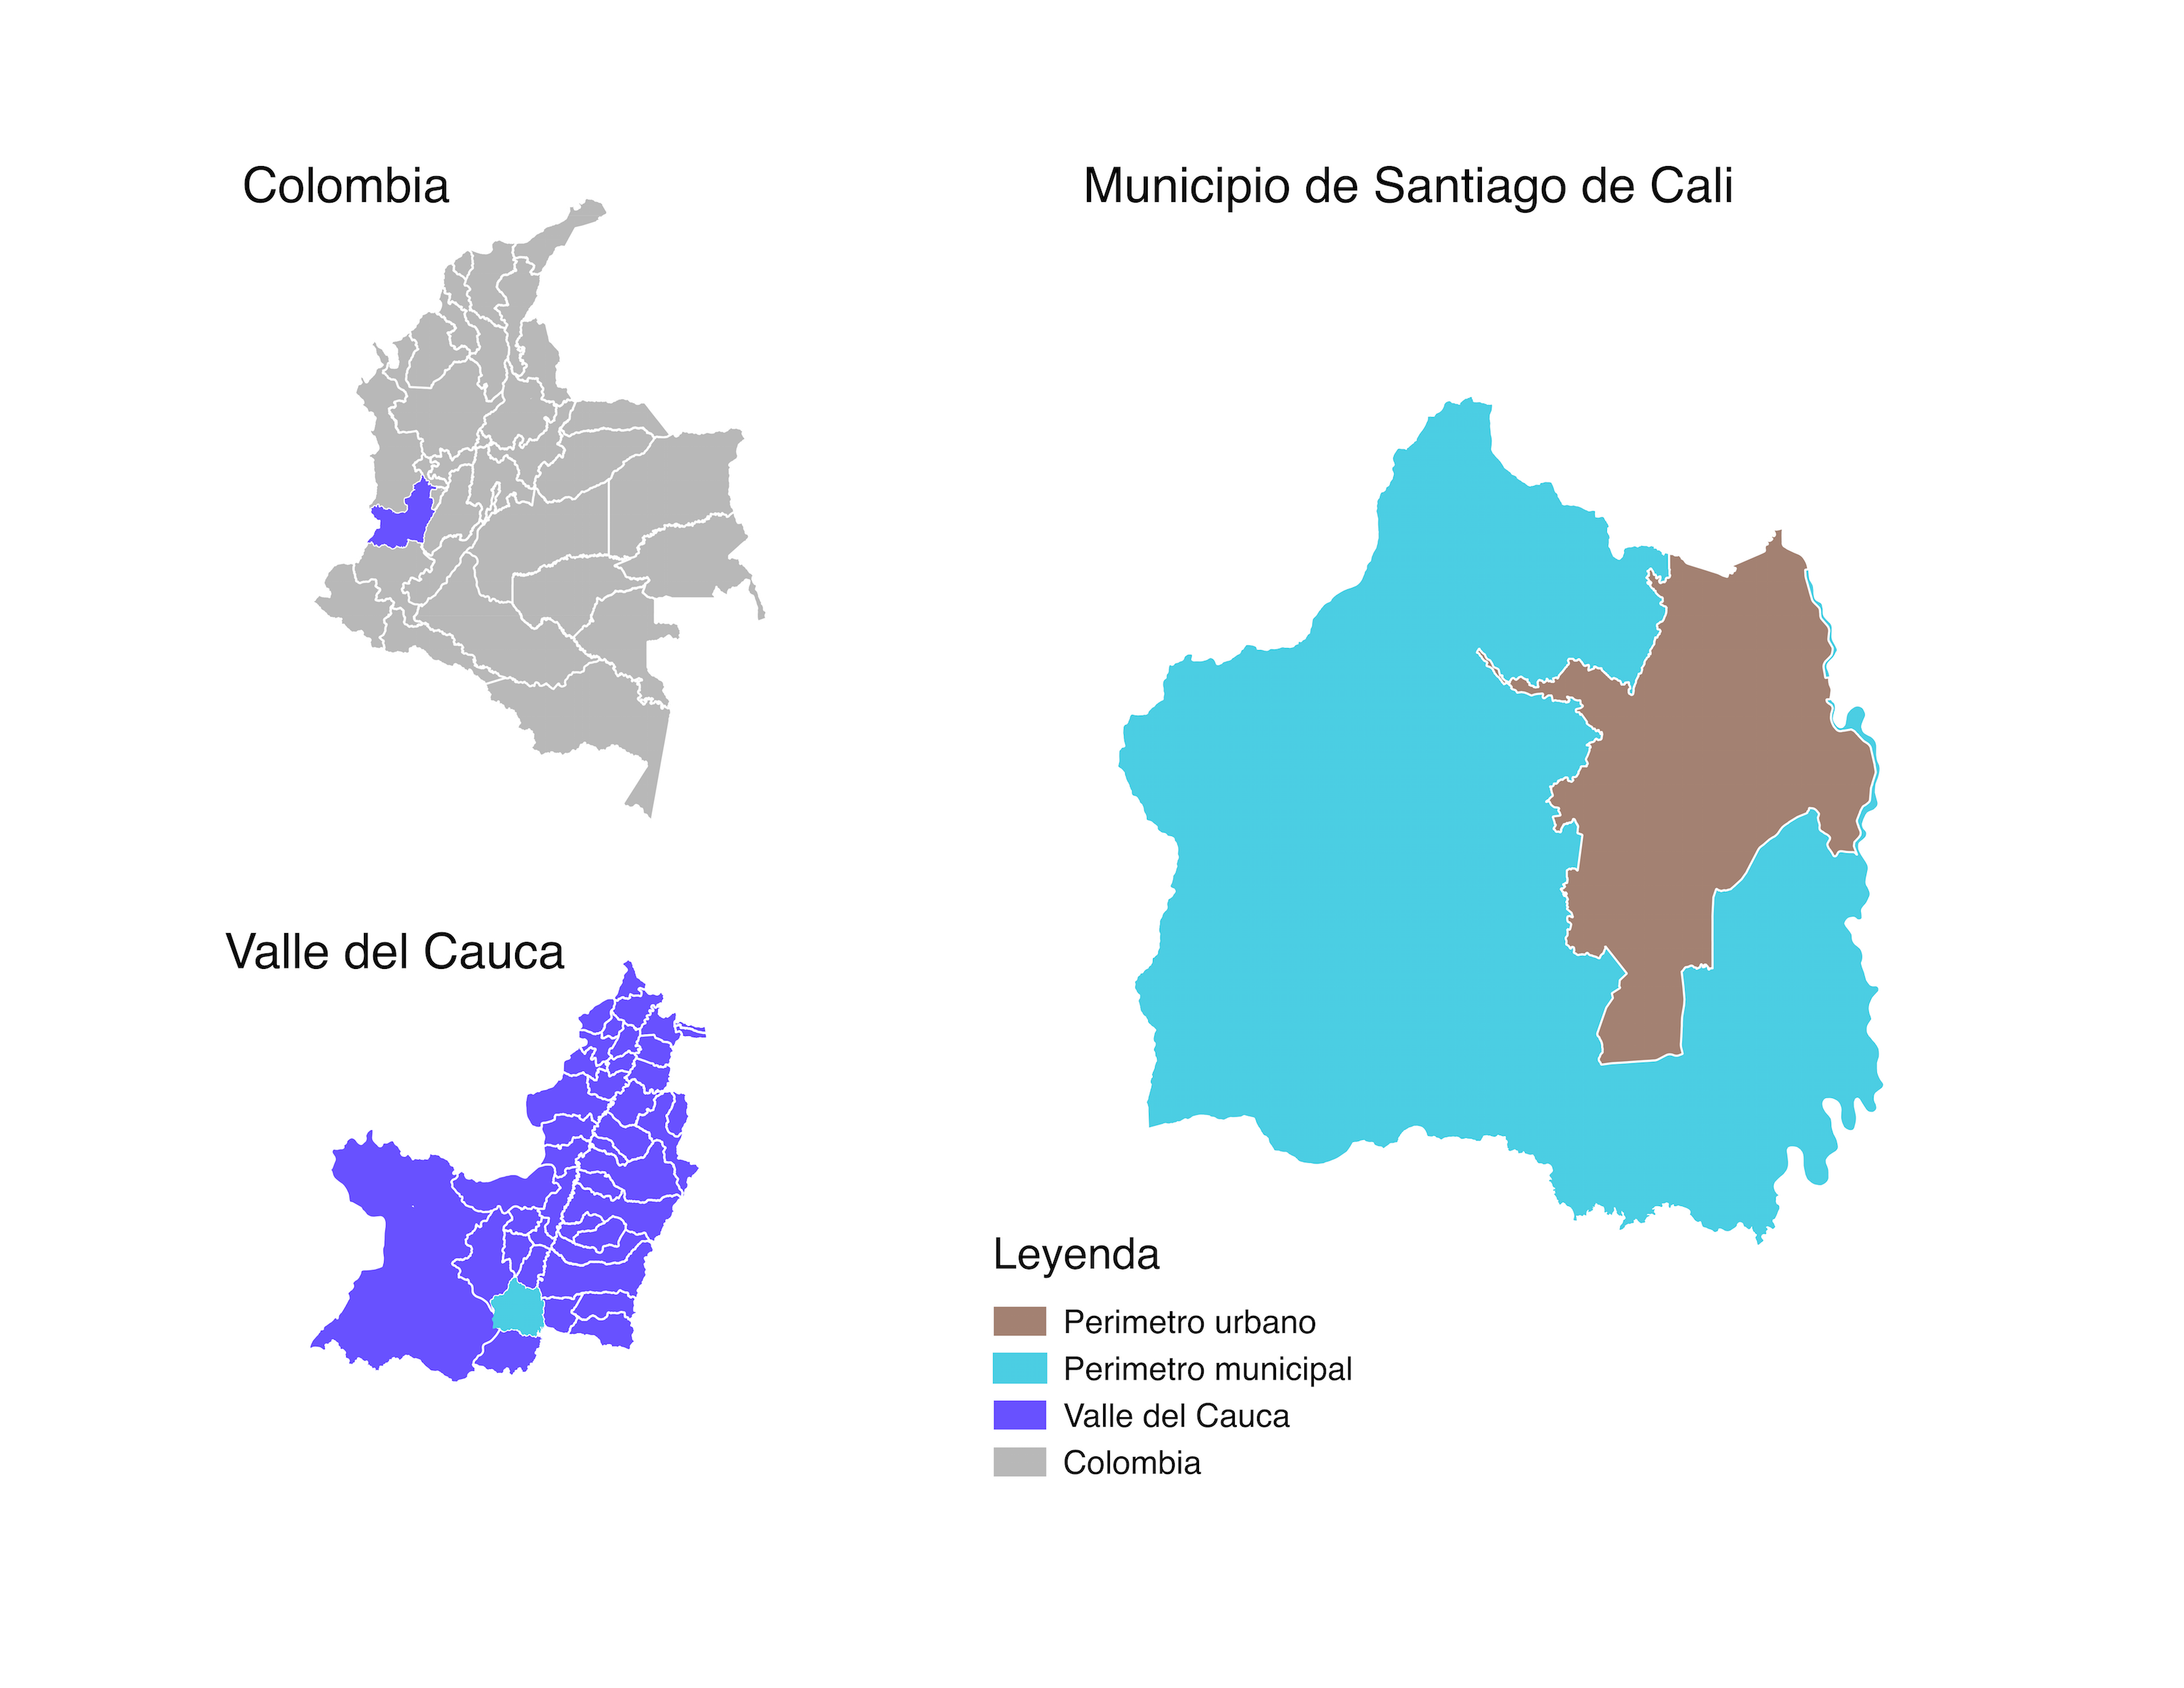
\includegraphics[width=1\linewidth]{QGIS/mapas/ubicacion_cali_low} \caption{Área de estudio}\label{fig:ubicacion}
\end{figure}

Santiago de Cali presenta dos zonas topográficas: el valle del río Cauca
hacia el oriente, el terreno más plano donde se ubica el casco urbano, y
la zona de piedemonte hacia el occidente sobre la margen derecha de la
cordillera Occidental. El area urbana limita al oeste y sur con el área
rural del municipio, al este con el río Cauca y los municipios de
Palmira y Candelaria, y al norte con el municipio de Yumbo.

\begin{figure}
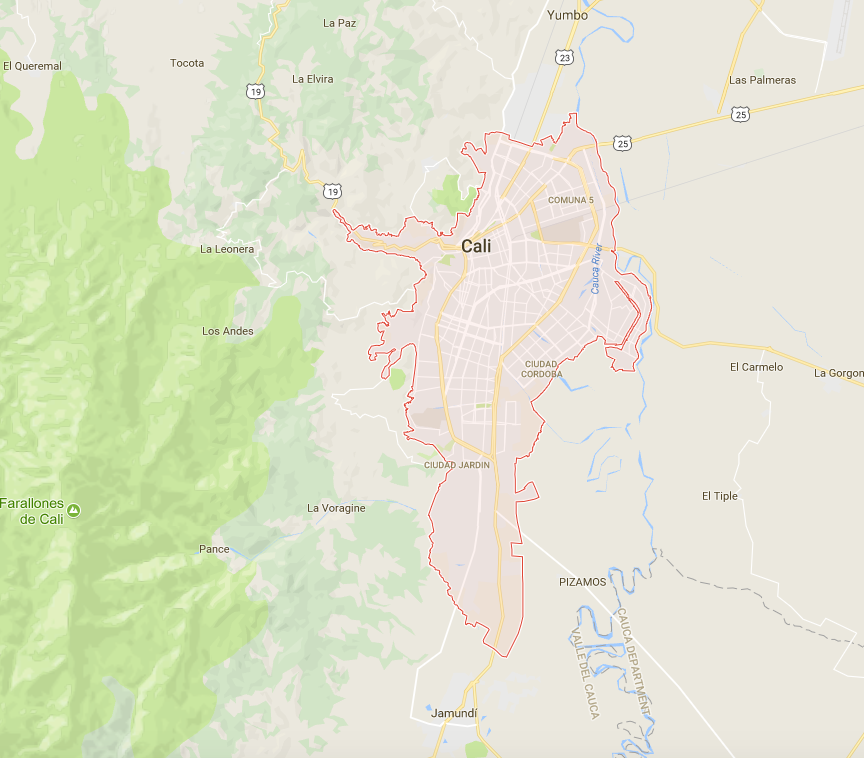
\includegraphics[width=1\linewidth]{images/googlemap} \caption{Mapa de Santiago de Cali,tomada de Google Maps}\label{fig:googlemp}
\end{figure}

El clima del municipio varía en relación al rango altitudinal que abarca
entre 916 y 1,438 msnm. En la zona plana, se presenta un clima cálido
con características semihúmedas hacia el sur y semiáridas hacia el norte
mientras el piedemonte presenta condiciones de clima templado. La
precipitación anual promedio es de 1.500 mm y la temperatura promedio
anual es de 24 °C aproximadamente. (CIAT, 2015). La ciudad de Cali es de
clima caliente, donde la sombra y la brisa son bien valoradas por sus
habitantes.

\begin{figure}
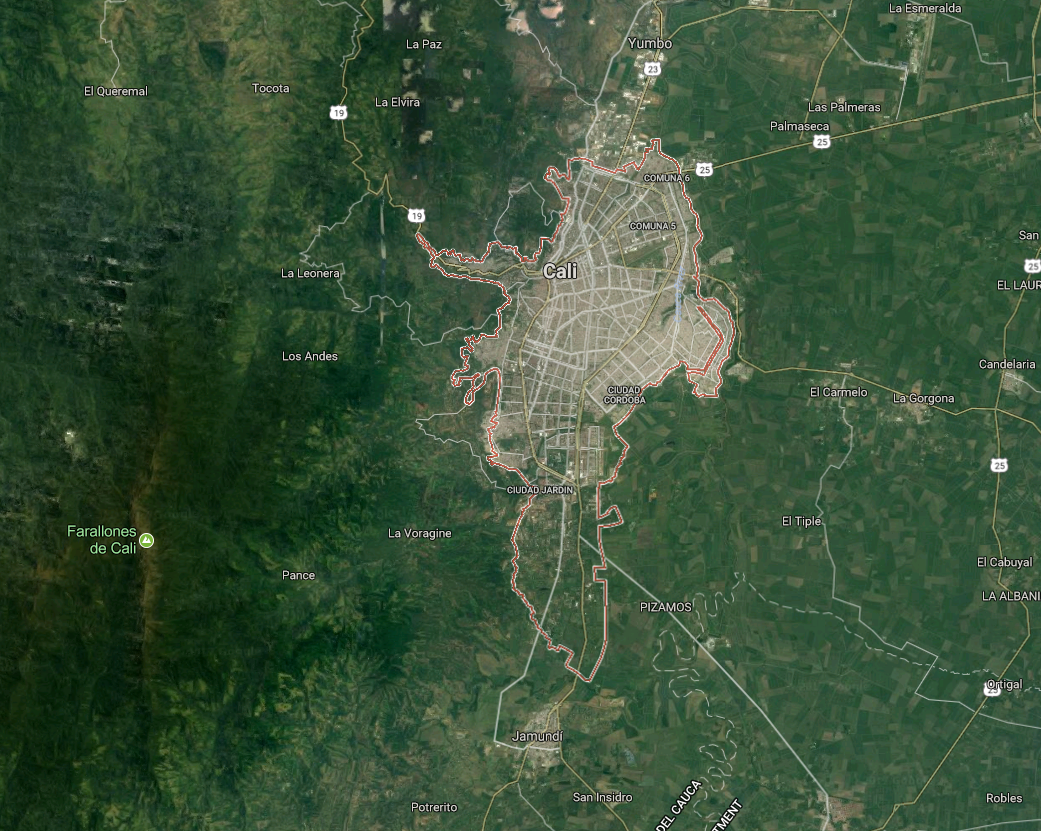
\includegraphics[width=1\linewidth]{images/satelite} \caption{Vista satelital de Santiago de Cali,tomada de Google Maps}\label{fig:satelite}
\end{figure}

\section{Datos}\label{datos}

\subsection{Datos de registros oficiales del
municipio}\label{datos-de-registros-oficiales-del-municipio}

La cartografía disponible en la Infraestructura de Datos Espaciales de
Santiago de Cali, IDESC \citep{geoportal_idesc}, incluye información
sobre los objetos geográficos naturales, de infraestructura urbana,
límites y divisiones político administrativas y la clasificación de
predios en cuanto a espacio público disponibles en coordenadas planas
del sistema \citep{noauthor_magna-sirgas-cali_nodate}. Además está la
base de datos geográfica del Plan de Ordenamiento territorial de Cali
2014, POT2014\footnote{Toda la información del POT2014 se encuentra en
  la web de la Alcaldía y puede descargarse como archivo GDB compatible
  con ArcGIS 10.4 o consumirse de Geoserver de IDESC como WFS o mapas en
  formato pdf del acuerdo}. Del POT2014 se seleccionaron conjuntos de
datos de equipamientos y espacio público contenido en la estructura
ecológica complementaria (ECC) que incluye cementerios, universidades,
EV de acceso no restringido aunque algunos sea predios privados
contenidos en EEC. De la IDESC se seleccionó la capa de barrios, espacio
público, humedales, ríos y corredores ambientales disponibles vía WFS.

En la figura \ref{fig:capas-idesc} se muestra un mapa con las capas
seleccionadas para el realizar el procesamiento y los análisis.

\begin{figure}
\includegraphics[width=1\linewidth]{images/capas_idesc_pot2014} \caption{Capas usadas para el procesamiento de los espacios verdes y las carateristicas de las manzanas}\label{fig:capas-idesc}
\end{figure}

\subsection{El censo arbóreo}\label{el-censo-arboreo}

En el año 2015 la ciudad de Santiago de Cali (Colombia) concretó la
realización de un censo arbóreo que dejó como resultado una base de
datos de aproximadamente 290.000 individuos censados. Los datos dan
cuenta de la identificación de especies, sus características
dasométricas, de emplazamiento y estado fitosanitario. Estos datos
constituyen un insumo fundamental para para la caracterización de los
beneficios y cargas que supone el mantenimiento y desarrollo del
arbolado urbano. De hecho, su realización ocurre en el marco del proceso
de formulación del plan silvicultura urbana o estatuto arbóreo\footnote{El
  proyecto de censo arbóreo se formuló en dos fases; la primera se
  ejecutó mediante convenio No 095 de 2013 entre la CVC y la Universidad
  Autónoma de Occidente, y la segunda fase mediante convenio No 049 de
  2014 entre las mismas entidades. Los datos no se encuentran publicados
  y fueron solicitados mediante un derecho de petición.} (Acuerdo 0335
de 2013). Las variables biofísicas recolectadas y la georeferenciación
de los individuos permite agregar las características del arbolado a
diferentes escalas de las unidades administrativas p.e divisiones
censales, para identificar y caracterizar su distribución espacial y
correlación con variables sociales o/y económicas. Las variables
seleccionadas se resumen en la tabla \ref{tab:vars-AU} y en la tabla
\ref{tab:datos-ca2015}.

\begin{longtable}[]{@{}rr@{}}
\caption{\label{tab:vars-AU} Variables para caracterizar el
AU}\tabularnewline
\toprule
\begin{minipage}[b]{0.09\columnwidth}\raggedleft\strut
variable\strut
\end{minipage} & \begin{minipage}[b]{0.38\columnwidth}\raggedleft\strut
\{valores\}{[}unidades{]}\strut
\end{minipage}\tabularnewline
\midrule
\endfirsthead
\toprule
\begin{minipage}[b]{0.09\columnwidth}\raggedleft\strut
variable\strut
\end{minipage} & \begin{minipage}[b]{0.38\columnwidth}\raggedleft\strut
\{valores\}{[}unidades{]}\strut
\end{minipage}\tabularnewline
\midrule
\endhead
\begin{minipage}[t]{0.09\columnwidth}\raggedleft\strut
id\_arbol\strut
\end{minipage} & \begin{minipage}[t]{0.38\columnwidth}\raggedleft\strut
número entero único\strut
\end{minipage}\tabularnewline
\begin{minipage}[t]{0.09\columnwidth}\raggedleft\strut
diametro copa\strut
\end{minipage} & \begin{minipage}[t]{0.38\columnwidth}\raggedleft\strut
{[}m\textsuperscript{2}{]}\strut
\end{minipage}\tabularnewline
\begin{minipage}[t]{0.09\columnwidth}\raggedleft\strut
altura arbol\strut
\end{minipage} & \begin{minipage}[t]{0.38\columnwidth}\raggedleft\strut
{[}m{]}\strut
\end{minipage}\tabularnewline
\begin{minipage}[t]{0.09\columnwidth}\raggedleft\strut
vitalidad\strut
\end{minipage} & \begin{minipage}[t]{0.38\columnwidth}\raggedleft\strut
\{Regular, Sano, Seco, Muerto\}\strut
\end{minipage}\tabularnewline
\begin{minipage}[t]{0.09\columnwidth}\raggedleft\strut
edad\strut
\end{minipage} & \begin{minipage}[t]{0.38\columnwidth}\raggedleft\strut
\{Juvenil, Maduro, Longevo\}\strut
\end{minipage}\tabularnewline
\begin{minipage}[t]{0.09\columnwidth}\raggedleft\strut
emplazamiento\strut
\end{minipage} & \begin{minipage}[t]{0.38\columnwidth}\raggedleft\strut
\{Anden, Bahias de estacionamiento, Bulevares, Corredor Ferreo,
Escenario deportivo y/o Cultural, Glorieta, Parque Urbano, Paseos,
Plaza, Plazoleta, Ronda de rios, Rondas de canales, Separador
Vial\}\strut
\end{minipage}\tabularnewline
\begin{minipage}[t]{0.09\columnwidth}\raggedleft\strut
vegetación\strut
\end{minipage} & \begin{minipage}[t]{0.38\columnwidth}\raggedleft\strut
\{Arbol, Arbusto, Bambu, Muerto, Palma, Planta arbustiva, Seco\}\strut
\end{minipage}\tabularnewline
\begin{minipage}[t]{0.09\columnwidth}\raggedleft\strut
Este\strut
\end{minipage} & \begin{minipage}[t]{0.38\columnwidth}\raggedleft\strut
{[}m{]} MAGNA - SIRGAS-CALI\strut
\end{minipage}\tabularnewline
\begin{minipage}[t]{0.09\columnwidth}\raggedleft\strut
Norte\strut
\end{minipage} & \begin{minipage}[t]{0.38\columnwidth}\raggedleft\strut
{[}m{]} MAGNA - SIRGAS-CALI\strut
\end{minipage}\tabularnewline
\bottomrule
\end{longtable}

\begin{table}

\caption{\label{tab:datos-ca2015}Muestra de los datos del censo arbóreo}
\centering
\begin{tabular}[t]{r|r|r|r|r|r}
\hline
id & vegetacion & edad & emplazamiento & diametro\_copa & altura\_arbol\\
\hline
0199G41070768 & Arbol & Maduro & Ronda de rios & 12 & 11\\
\hline
0199G41070769 & Arbol & Maduro & Ronda de rios & 7 & 8\\
\hline
0199G41070770 & Arbol & Maduro & Ronda de rios & 5 & 3\\
\hline
0199G41070771 & Arbol & Maduro & Ronda de rios & 6 & 7\\
\hline
0199G41070772 & Arbol & Maduro & Ronda de rios & 9 & 8\\
\hline
0199G41070773 & Arbol & Maduro & Ronda de rios & 10 & 7\\
\hline
\end{tabular}
\end{table}

Los árboles incluidos en el censo arbóreo de 2015 están separados por 10
años de los datos de caracterización socioeconómica y de la
características de ocupación de los sectores urbanos. Esta brecha puede
cerrarse un poco excluyendo los árboles catalogados como jóvenes. Otro
factor que ayuda a matizar la distancia entre los datos de ambos censos
es que el AU se desarrolla lento y los tamaños actuales de las copas y
las alturas de los árboles, aunque son mayores que en el 2005, hablan
del potencial que desarrollaron esas zonas. Dado que esa es la
disponibilidad de datos poblacionales hay que asumir estas diferencias.
Finalmente, para este trabajo usaremos árboles, palmas y bambú de más de
1.9 m de altura (descartando arbustos y plantas arbustivas) para
garantizar que son individuos que proveen sombra a los transeúntes.

En la siguiente figura \ref{fig:capa-ca2015sel} se observa todos los
arboles seleccionados para el analsis.

\begin{figure}
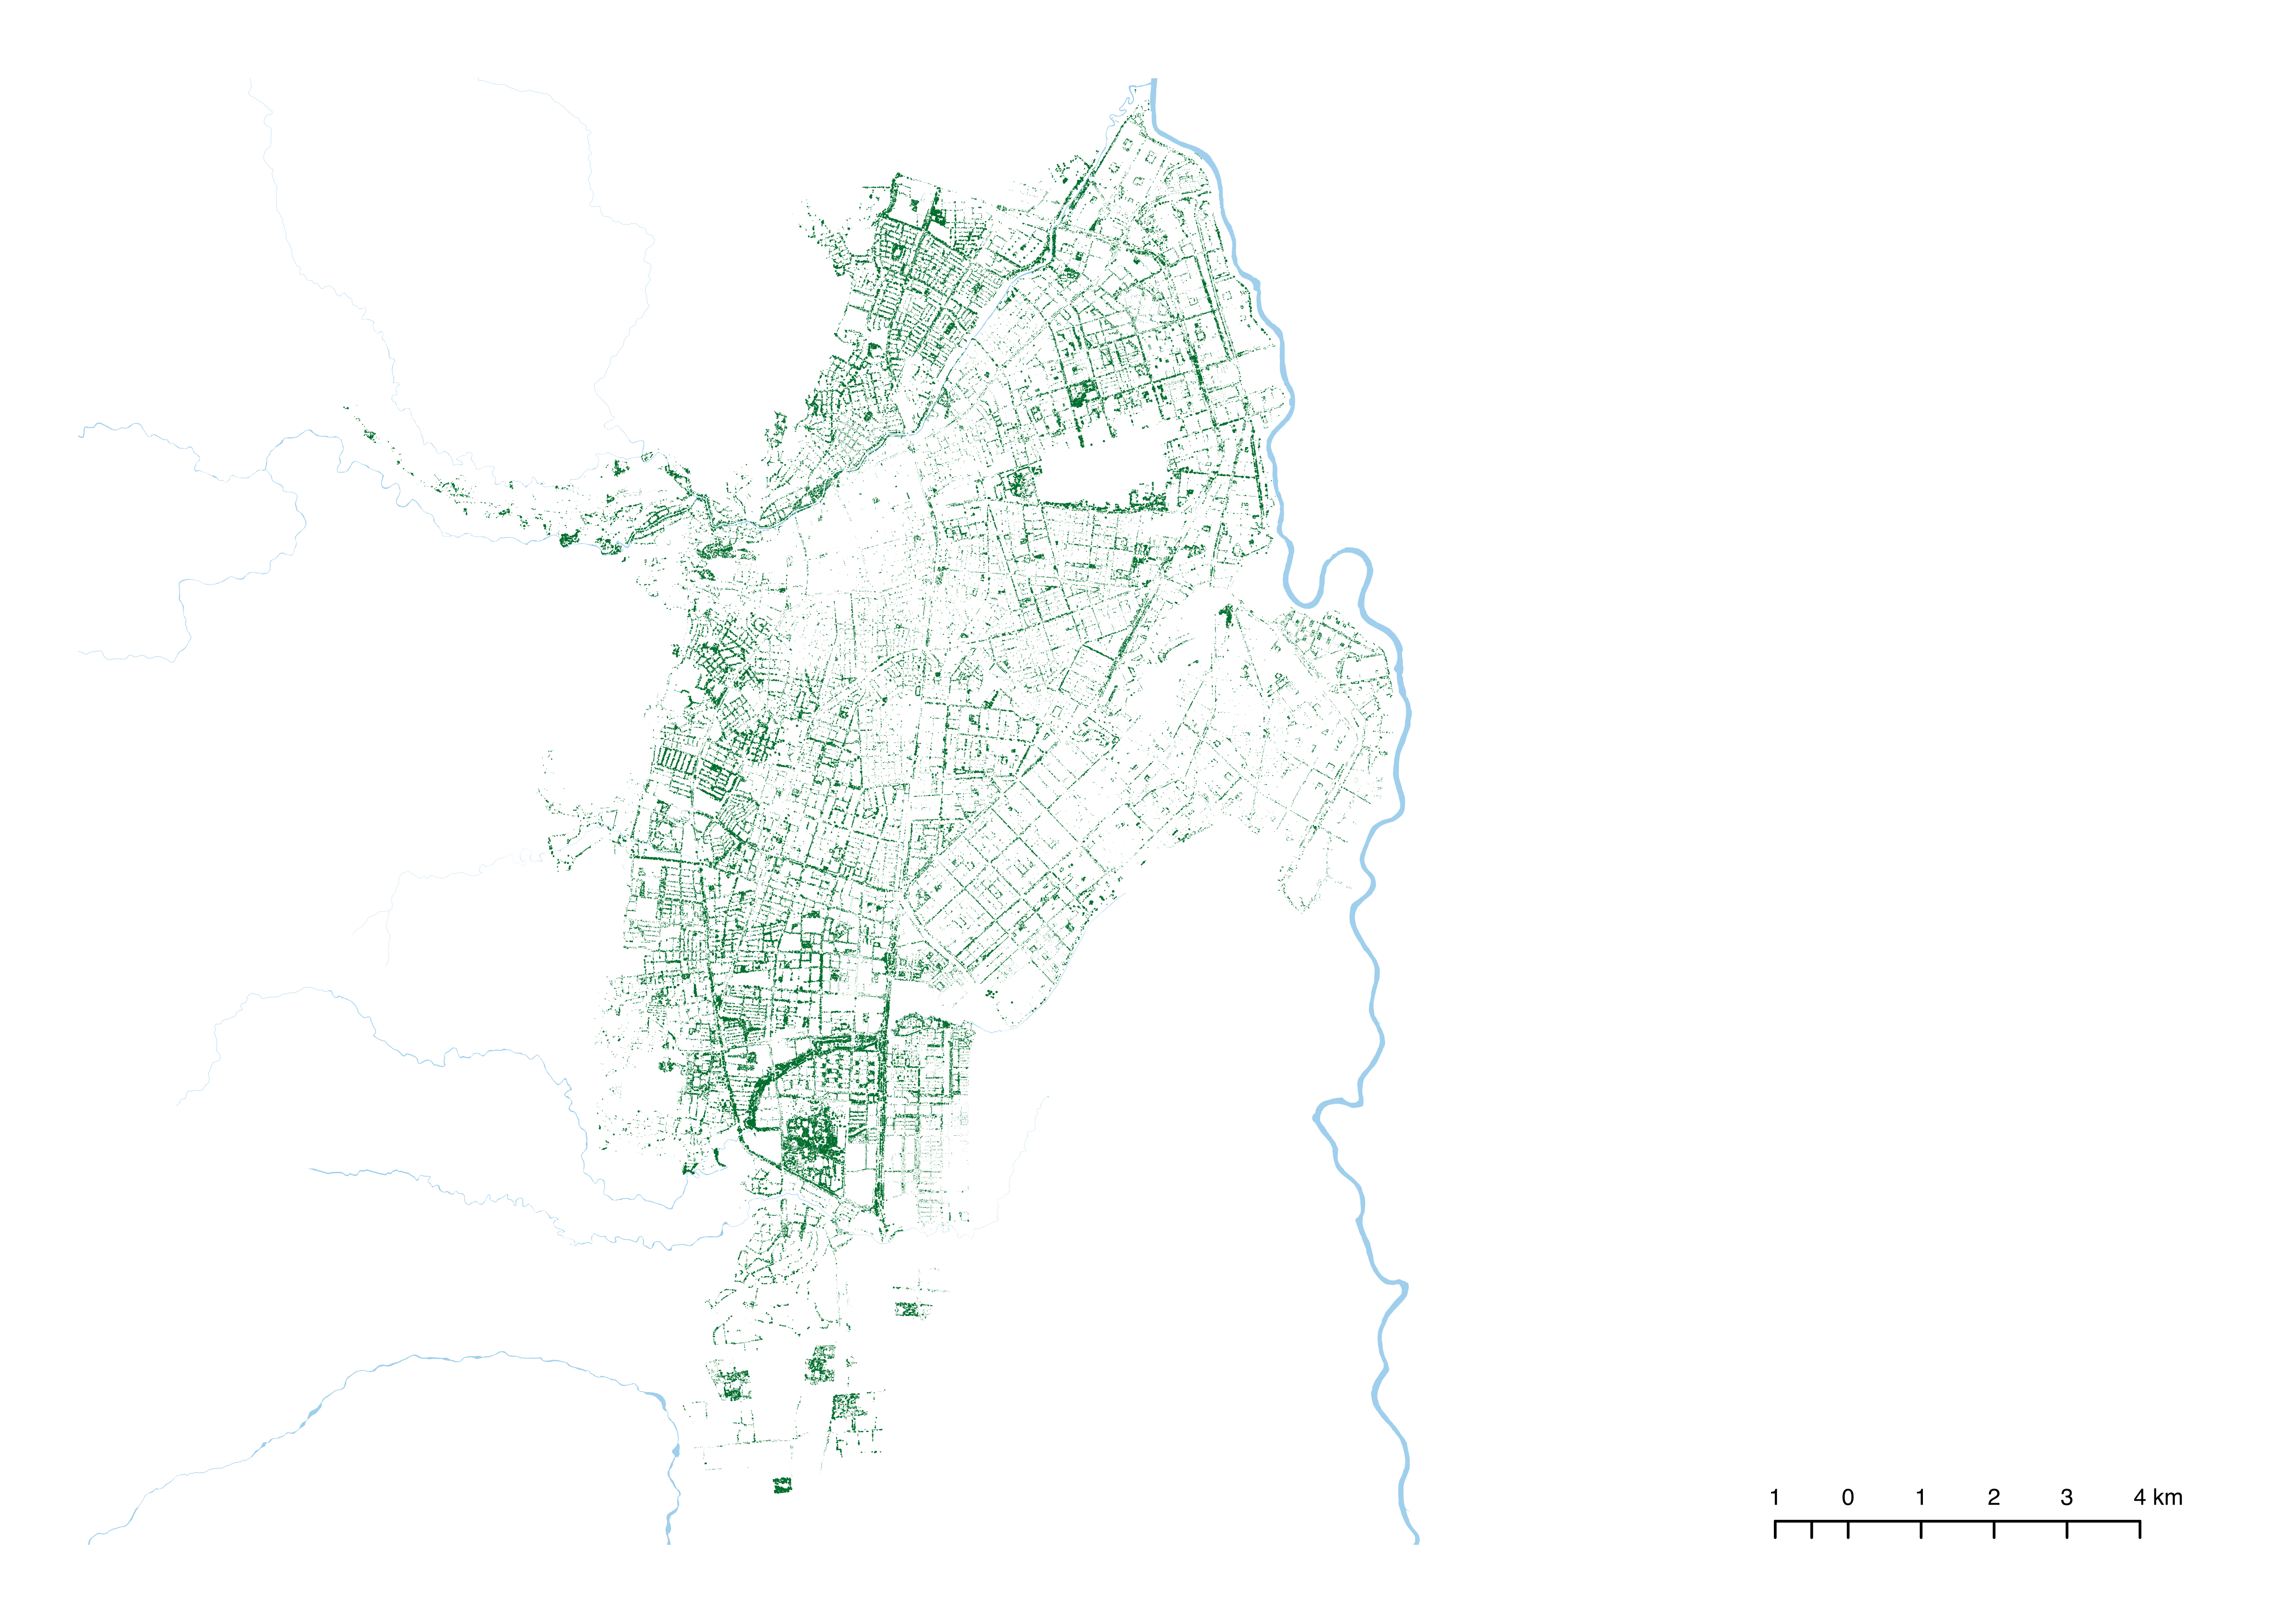
\includegraphics[width=1\linewidth]{images/arboles_sombra} \caption{Árboles seleccionados para el análisis. El tamaño de puntos que representan los arboles es proporcional al area de la copa en unidades del mapa.}\label{fig:capa-ca2015sel}
\end{figure}

\subsection{El censo de población}\label{el-censo-de-poblacion}

El último censo de población en Colombia se realizó en el año 2005, y
los datos se pueden consultar y agregar en las diferentes unidades
censales (sector, sección, manzana) usando una sistema de consulta web
de censos Redatam\footnote{El sistema de consulta es el
  \citep{cepal_redatam_nodate}, que se puede acceder directamente desde
  \citep{dane_cepal_celade_2005} y en la página web del
  \href{http://www.dane.gov.co/index.php/estadisticas-por-tema/demografia-y-poblacion/censo-general-2005-1}{DANE}
  dónde está organizada la documentación metodológica y otros servicios
  del censo.}. Estos datos sirven para caracterizar la población con
base en indicadores y rasgos de las personas, aspectos sobre el uso del
suelo y los tipos de vivienda. Las variables disponibles para el
análisis están resumidas en las tablas \ref{tab:vars-poblacion} y
\ref{tab:vars-vivienda}.

El otro componente de los datos es la cartografía censal del DANE
\citep{geoportal_DANE} disponible para las diferentes unidades
espaciales de agregación en el sistema de coordenadas WGS84. Para el
análisis se tiene en cuenta todos las unidades censales que se
interceptan con el perímetro urbano disponible en la IDESC, pues el
censo arboreo se limito al este prerímetro.(ver figura
\ref{fig:su-periurbano})

\begin{longtable}[]{@{}rr@{}}
\caption{\label{tab:vars-poblacion} Variables sobre la
población}\tabularnewline
\toprule
\begin{minipage}[b]{0.09\columnwidth}\raggedleft\strut
variable\strut
\end{minipage} & \begin{minipage}[b]{0.38\columnwidth}\raggedleft\strut
\{valores\}{[}unidades{]}\strut
\end{minipage}\tabularnewline
\midrule
\endfirsthead
\toprule
\begin{minipage}[b]{0.09\columnwidth}\raggedleft\strut
variable\strut
\end{minipage} & \begin{minipage}[b]{0.38\columnwidth}\raggedleft\strut
\{valores\}{[}unidades{]}\strut
\end{minipage}\tabularnewline
\midrule
\endhead
\begin{minipage}[t]{0.09\columnwidth}\raggedleft\strut
Pertenencia Étnica\strut
\end{minipage} & \begin{minipage}[t]{0.38\columnwidth}\raggedleft\strut
{[}personas{]}\{indígenas, ROM, gitanos, raizales del Archipiélago de
San Andrés, Providencia y Santa Catalina, palenqueros de San Basilio,
afrocolombianos\}\strut
\end{minipage}\tabularnewline
\begin{minipage}[t]{0.09\columnwidth}\raggedleft\strut
Con alguna limitación\strut
\end{minipage} & \begin{minipage}[t]{0.38\columnwidth}\raggedleft\strut
{[}personas{]}\{sí,no\}\strut
\end{minipage}\tabularnewline
\begin{minipage}[t]{0.09\columnwidth}\raggedleft\strut
Con estudios superior o postgrado\strut
\end{minipage} & \begin{minipage}[t]{0.38\columnwidth}\raggedleft\strut
{[}personas{]}\strut
\end{minipage}\tabularnewline
\begin{minipage}[t]{0.09\columnwidth}\raggedleft\strut
Ningún estudio\strut
\end{minipage} & \begin{minipage}[t]{0.38\columnwidth}\raggedleft\strut
{[}personas{]}\strut
\end{minipage}\tabularnewline
\bottomrule
\end{longtable}

\begin{figure}
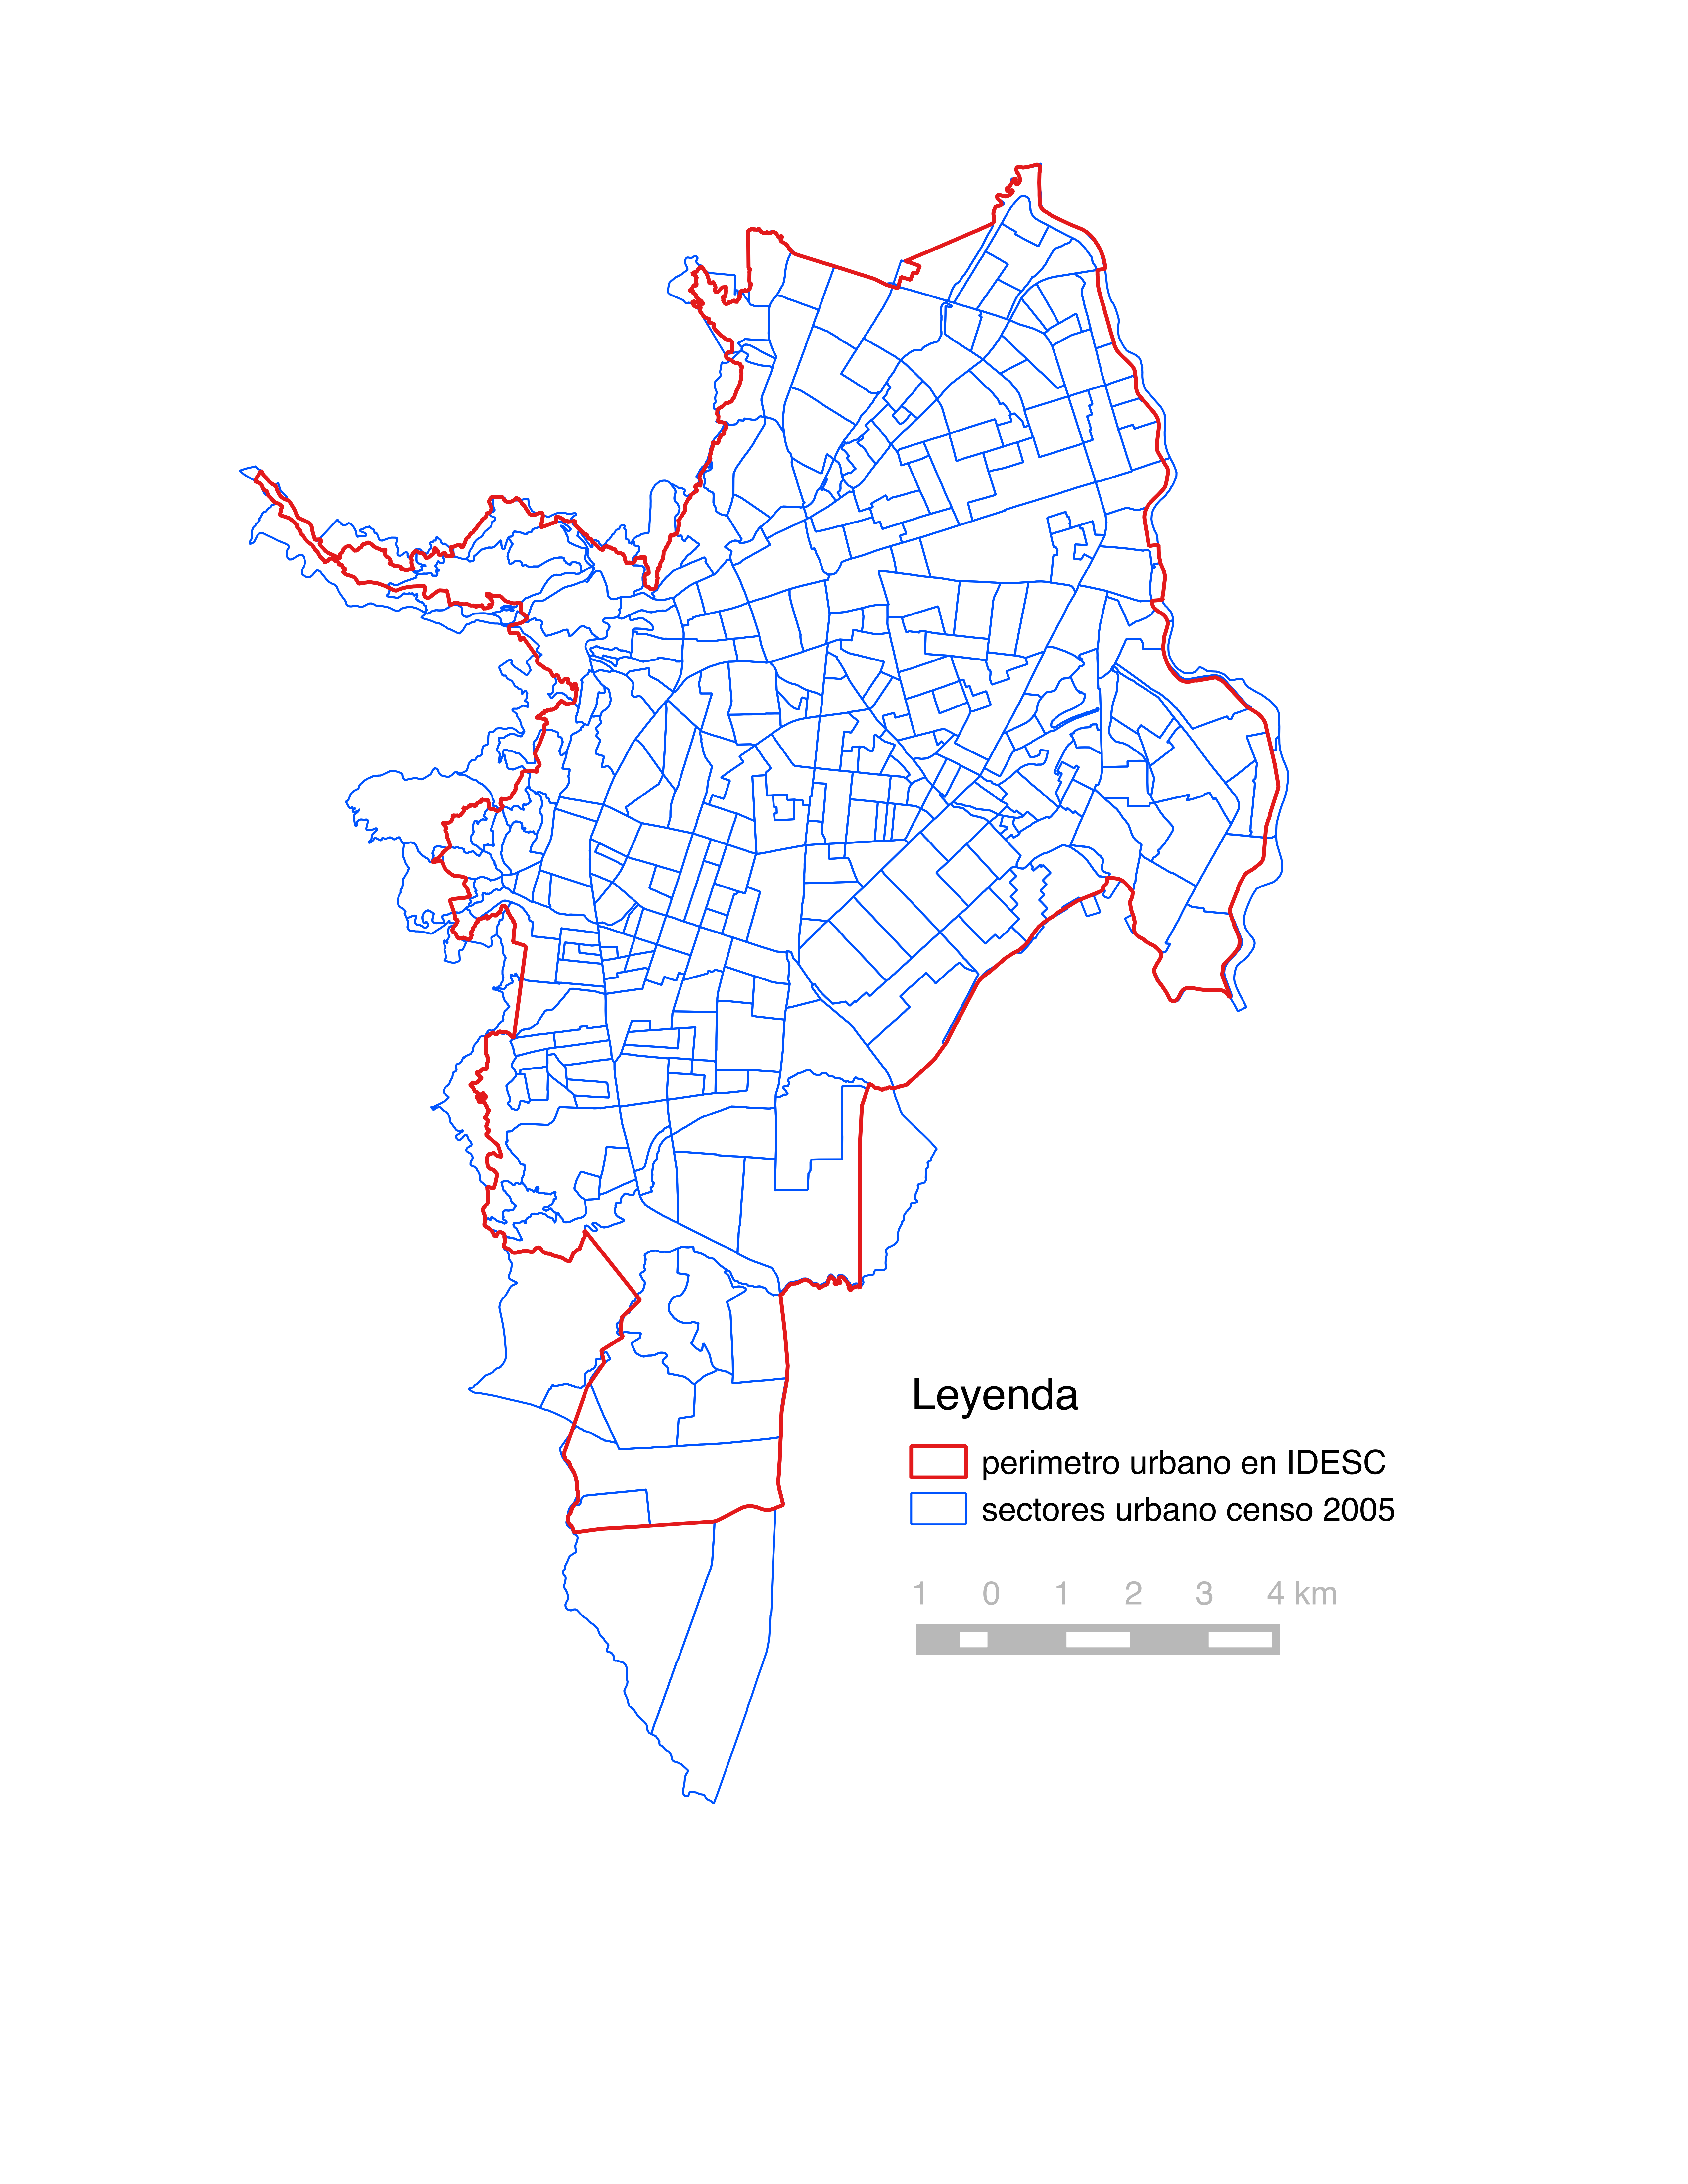
\includegraphics[width=1\linewidth]{images/sectoresurbanos_perimetro_idesc} \caption{División en barrios y sectores urbanos de Santiago de Cali}\label{fig:su-periurbano}
\end{figure}

\begin{longtable}[]{@{}rr@{}}
\caption{\label{tab:vars-vivienda} Variables sobre la las
viviendas}\tabularnewline
\toprule
\begin{minipage}[b]{0.09\columnwidth}\raggedleft\strut
variable\strut
\end{minipage} & \begin{minipage}[b]{0.38\columnwidth}\raggedleft\strut
\{valores\}{[}unidades{]}\strut
\end{minipage}\tabularnewline
\midrule
\endfirsthead
\toprule
\begin{minipage}[b]{0.09\columnwidth}\raggedleft\strut
variable\strut
\end{minipage} & \begin{minipage}[b]{0.38\columnwidth}\raggedleft\strut
\{valores\}{[}unidades{]}\strut
\end{minipage}\tabularnewline
\midrule
\endhead
\begin{minipage}[t]{0.09\columnwidth}\raggedleft\strut
tipo vivienda\strut
\end{minipage} & \begin{minipage}[t]{0.38\columnwidth}\raggedleft\strut
{[}viviendas{]} \{Casa,Casa indígena,Apartamento,Tipo cuarto,Otro tipo
de vivienda\}\strut
\end{minipage}\tabularnewline
\begin{minipage}[t]{0.09\columnwidth}\raggedleft\strut
uso vivienda\strut
\end{minipage} & \begin{minipage}[t]{0.38\columnwidth}\raggedleft\strut
{[}predio{]}\{Uso Vivienda.Uso Unidad Económica,Uso LEA\}\strut
\end{minipage}\tabularnewline
\begin{minipage}[t]{0.09\columnwidth}\raggedleft\strut
cantidad predios\strut
\end{minipage} & \begin{minipage}[t]{0.38\columnwidth}\raggedleft\strut
{[}predios{]}\strut
\end{minipage}\tabularnewline
\begin{minipage}[t]{0.09\columnwidth}\raggedleft\strut
cantidad viviendas\strut
\end{minipage} & \begin{minipage}[t]{0.38\columnwidth}\raggedleft\strut
{[}viviendas{]}\strut
\end{minipage}\tabularnewline
\bottomrule
\end{longtable}

Una de las apuestas del proyecto es incluir aspectos de los procesos de
desarrollo urbano a través de la idea de barrio: como unidad de
identidad cultural urbana y estructural, de características físicas y
habitacionales en las que confluyen las transformaciones que hacen los
habitantes y los diseños urbanos e intervenciones arquitectónicas de los
planeadores y constructores en la ciudad. Sin embargo, la información
socioeconómica disponible está en unidades de la cartografía censal del
2005, que no coincide exactamente con los límites de barrios. Un primer
supuesto es que los sectores censales aproximan bien a los barrios, pues
las diferencias no tan drmaticas (ver figura \ref{fig:su-barrios}). La
unidad espacial de análisis sobre la cual se harán todas las
agregaciones el sector urbano (SU) de la cartografía censal 2005.

\begin{figure}
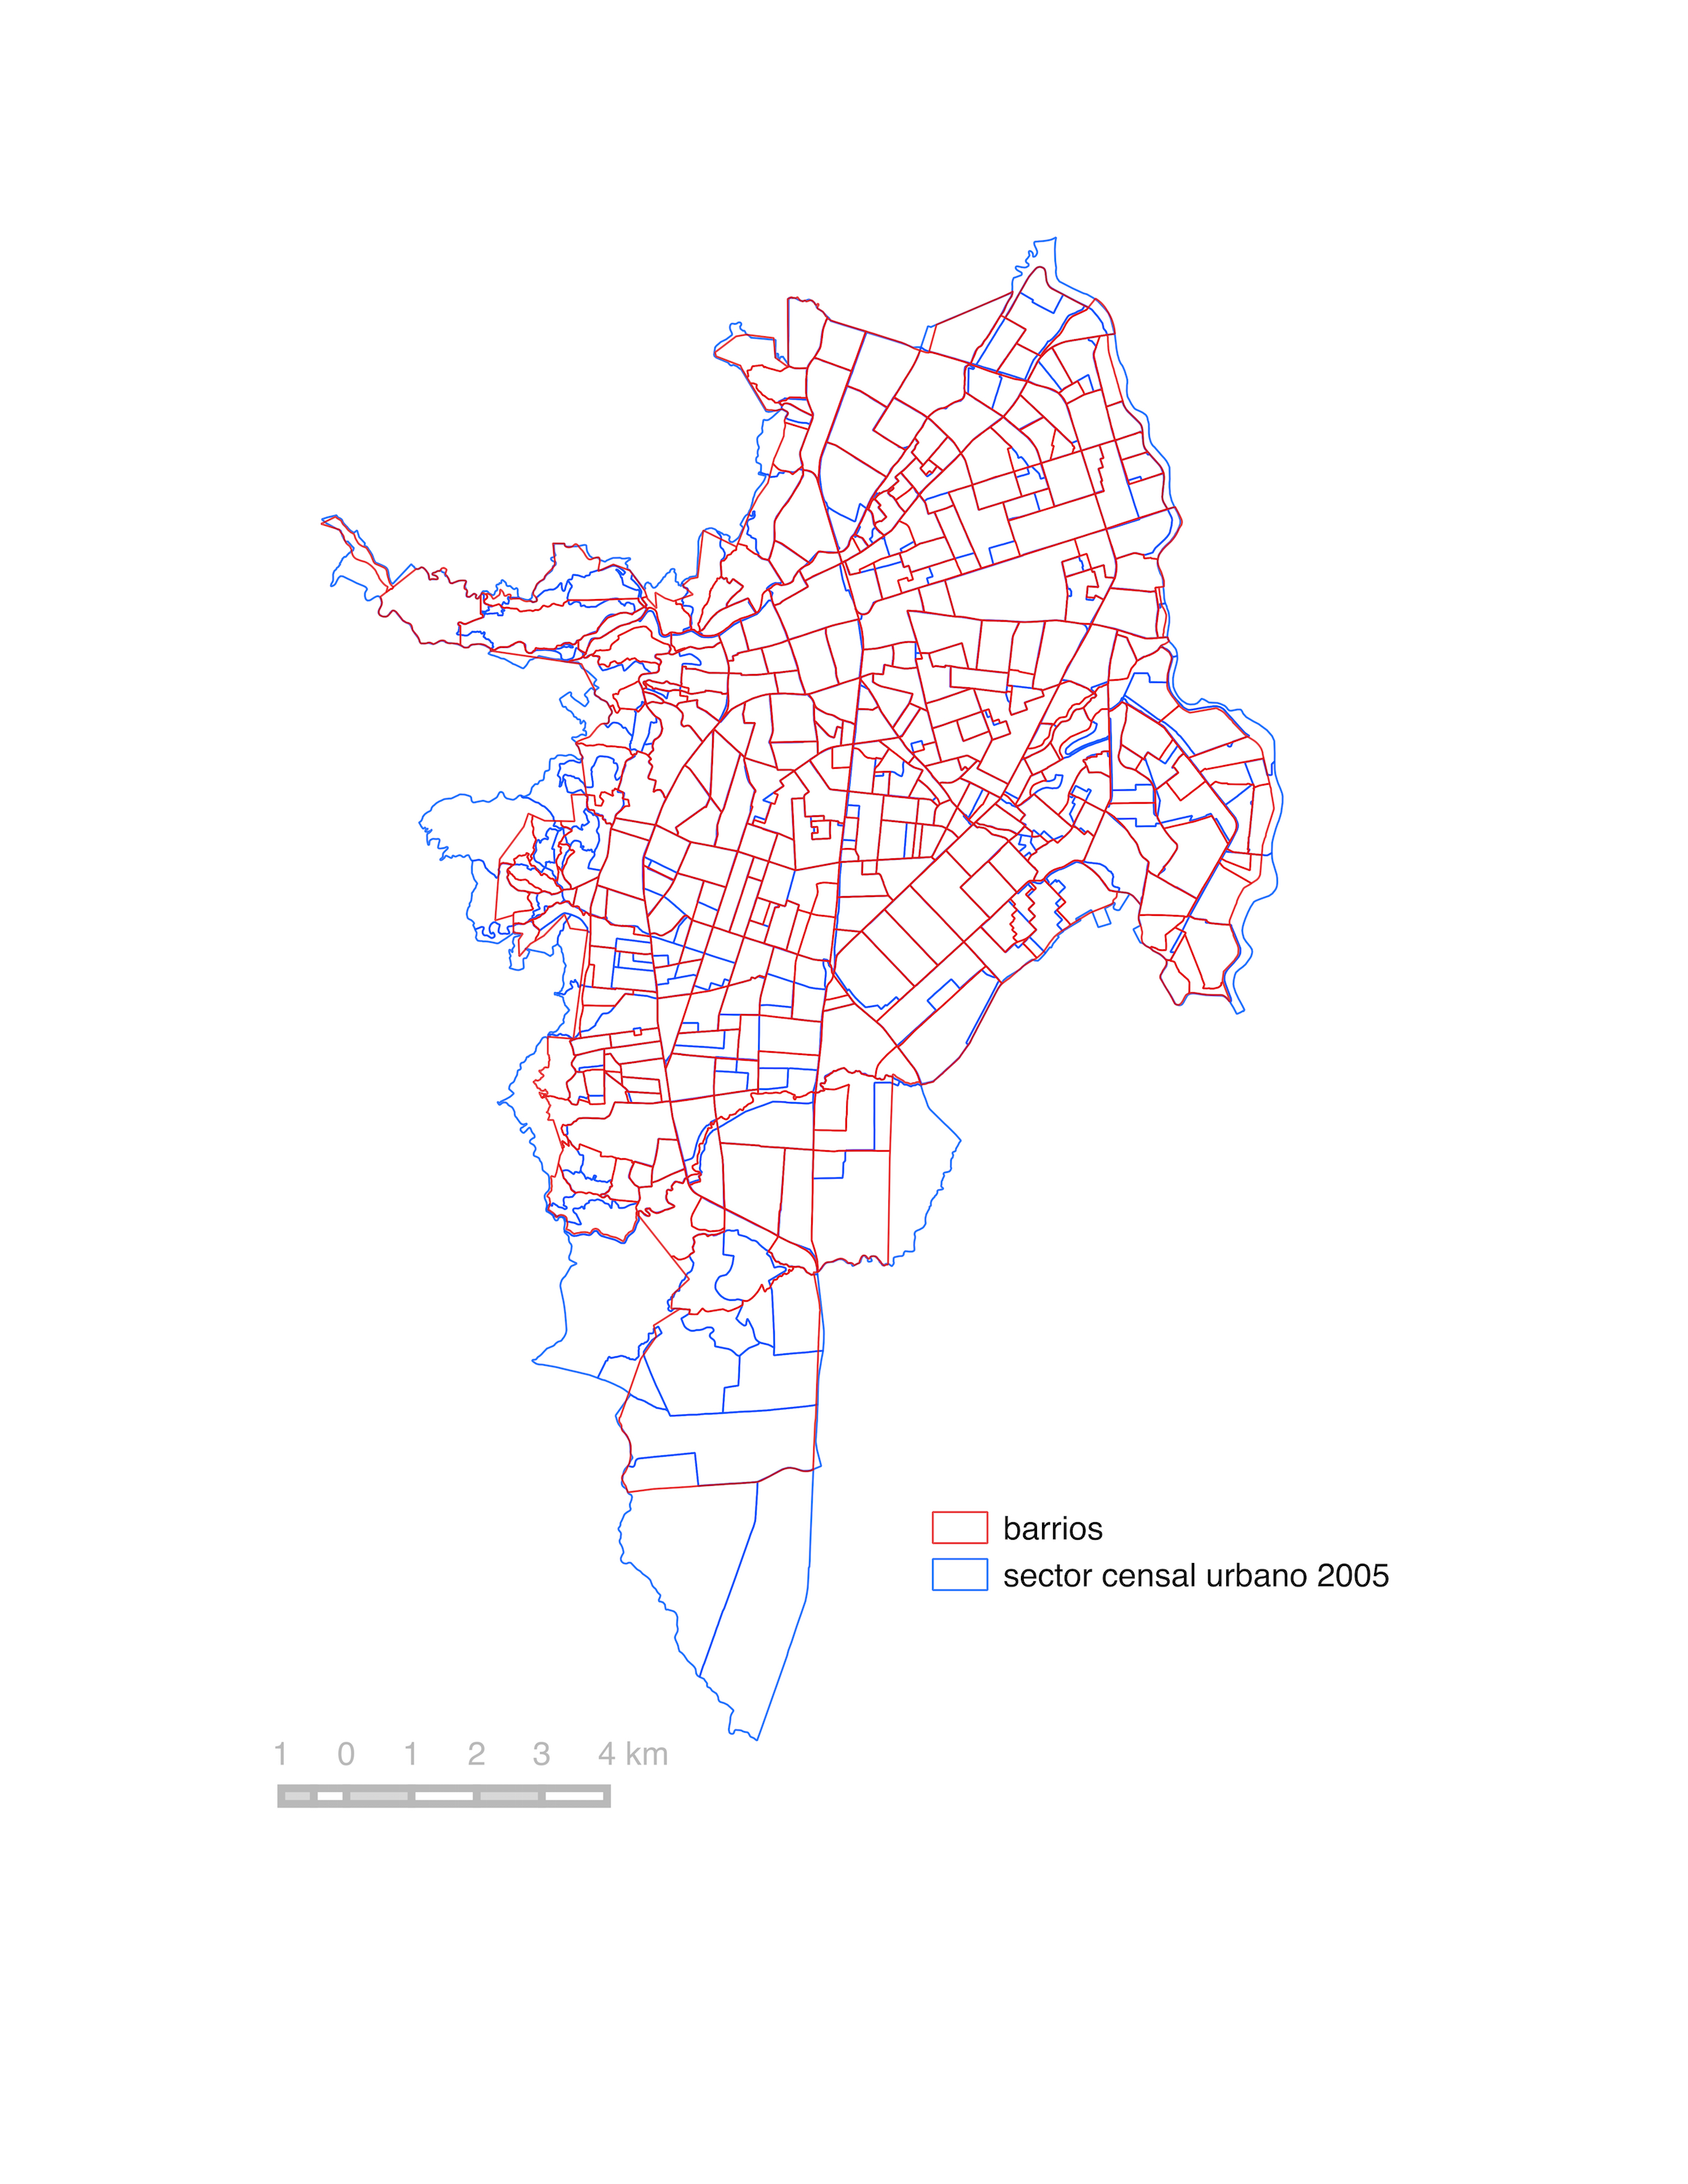
\includegraphics[width=1\linewidth]{images/barrio_sectorurbano} \caption{División en barrios y sectores urbanos de Santiago de Cali}\label{fig:su-barrios}
\end{figure}

Los demás conjuntos de datos, cuyos elementos sobrepasen los límites del
centro poblado conformado por los SUs seleccionados son preprocesados
para excluir los datos y zonas fuera del perímetro conformado por los
SUs.

\section{Métodos y técnicas}\label{metodos-y-tecnicas}

El análisis propuesto se compone de las siguientes actividades:

\begin{enumerate}
\def\labelenumi{\arabic{enumi}.}
\tightlist
\item
  Preparación de los datos: una tarea común pero crucial para el
  análisis de datos. La estandarización de las variables categóricas y
  la identificación de valores atípicos o inconsistentes es una base
  firme para la estimación de parámetros y obtener soluciones confiables
  y sensibles de interpretación. Los datos suelen estar usualmente en
  formatos para la lectura humana o con distinta estructura de las
  variables de los modelos. La preparación de los datos consume la mayor
  parte de los esfuerzos de las tareas de procesamiento de los datos.
  Los datos del censo arbóreo se encuentra en tablas bien conformadas lo
  que facilita su manipulación. Los datos de consulta del censo de
  población vienen en tablas independientes para cada unidad espacial
  seleccionada, con diferentes longitud de variables. A esto se suma el
  componente espacial, donde hay que prestar particular atención a los
  sistemas de coordenadas y usar coordenadas planas consistentes con las
  unidades de espacio.
\item
  Procesamiento y análisis estadístico: cálculo de indicadores de
  cobertura, acceso y variables socioeconómicas. Cálculo de estadísticos
  para probar normalidad, normalización de las variables e indicadores,
  cálculos de coeficientes de correlación Pearson y de Spearman entre
  todos los pares de variables.
\item
  Inspección visual de los datos: hacer uso de gráficas estadísticas,
  mapeos y mapas para evaluar y seleccionar los indicadores a usar en un
  modelo de regresión lineal.
\item
  Evaluar los residuos usando la prueba de correlación espacial de
  Moran'I usando al menos dos diseños de matriz W. Si la prueba muestra
  una correlación y un valor de significancia alta, se prueban modelos
  tipo SAR, SEM o SLX para comparar su desempeño.
\item
  Selección del modelo que mejor se ajusta usando métricas de error y de
  ajuste como R2 y el criterio de Akaike.
\end{enumerate}

\chapter{Procesamiento y análisis de datos}\label{anayproc}

El procesamiento de los datos se realizó principalmente en
\citet{R-base}. Se usó \href{http://www.qgis.org/es/site/}{QGIS} para
conectarse a los servicios WFS del IDESC y previsualizar las capas de
información geográfica recolectada y la realización de algunos de los
mapas detallados.

El código que implementa los análisis está dividido en archivos para
facilitar su lectura, cada uno de los cuales se encargan de transformar
los datos de las fuentes y construir estructuras de datos necesarias
para realizar las regresiones, las gráficas y los análisis de tipo
estadístico y geoestadístico. Cada script implementa una fase de la
metodología y produce resultados intermedios que facilitan seguir y
reproducir dichas transformaciones sobre los datos de un dominio del
problema. El archivo de \texttt{funciones.R} agrupa funciones que
encapsulan funcionalidades recurrentes dentro del desarrollo del
análisis. El script de \texttt{geodata.R} opera sobre los fuentes de
datos geográficas necesarias para consolidar los índices de acceso a
espacios verdes (EV), los indicadores y variables de la estructura de
física de los sectores censales y unidades geográficas del análisis. El
script \texttt{arboles,R} consolida la información de cada uno de los
individuos del censo arbóreo agregandolos por sector censal. El scrript
\texttt{censopoblacion.R} consolida los datos del Censo de Población
2005. Los scripts \texttt{consolidarDatos.R} y
\texttt{analisis\_exploratorio.R} consolidan una única estructura con
todos los datos y produce una serie de gráficas y medidas de
correlación, que son base para la identificación de supuestos y
selección de las variables independientes para los análisis estadísticos
y las regresiones espaciales. Finalmente los script de
\texttt{analisis\_estadistico.R} y \texttt{analisis\_geoestadistico.R}
implementan las regresiones lineales y las regresiones espaciales
respectivamente, así como los test y tablas para la verificación de los
supuesto matemáticos y la verificación de la calidad de los resultados.
Todos estos están reunidos en un script que carga las librerías
necesarias y ejecuta secuencialmente cada de los scripts descritos.

\begin{Shaded}
\begin{Highlighting}[]
\CommentTok{# Scrip principal para la la ejecución de los .R}

\CommentTok{# librerias}

\KeywordTok{library}\NormalTok{(rgdal)}
\KeywordTok{library}\NormalTok{(rgeos)}
\KeywordTok{library}\NormalTok{(raster)}
\KeywordTok{library}\NormalTok{(sp)}

\KeywordTok{library}\NormalTok{(tidyverse)}
\KeywordTok{library}\NormalTok{(magrittr)}
\KeywordTok{library}\NormalTok{(stringr)}

\KeywordTok{library}\NormalTok{(viridis)}
\KeywordTok{library}\NormalTok{(RColorBrewer)}
\KeywordTok{library}\NormalTok{(gridExtra)}

\KeywordTok{library}\NormalTok{(visdat)}
\KeywordTok{library}\NormalTok{(GGally)}
\KeywordTok{library}\NormalTok{(wesanderson)}

\KeywordTok{library}\NormalTok{(ggrepel)}


\CommentTok{# correr los script en el orden correcto para realizar todos los calculos}

\KeywordTok{source}\NormalTok{(}\StringTok{"funciones.R"}\NormalTok{)}
\KeywordTok{source}\NormalTok{(}\StringTok{"geodata.R"}\NormalTok{)}
\KeywordTok{source}\NormalTok{(}\StringTok{"arboles.R"}\NormalTok{)}
\KeywordTok{source}\NormalTok{(}\StringTok{"censopoblacion.R"}\NormalTok{)}
\KeywordTok{source}\NormalTok{(}\StringTok{"consolidarDatos.R"}\NormalTok{)}
\KeywordTok{source}\NormalTok{(}\StringTok{"analisis_exploratorio.R"}\NormalTok{)}
\KeywordTok{source}\NormalTok{(}\StringTok{"analisis_estadistico.R"}\NormalTok{)}
\KeywordTok{source}\NormalTok{(}\StringTok{"analisis_geoestadistico.R"}\NormalTok{)}
\end{Highlighting}
\end{Shaded}

\section{Capas de información
geográfica}\label{capas-de-informacion-geografica}

Para usar la información geográfica de la cartografía censal y la
información del IDESC es necesario establecer un sistema de coordenadas
común, en unidades métricas, que facilite integrar la información y
produzca resultados consistentes. El sistema de coordenadas proyectadas
que vamos a usar es \citet{noauthor_magna-sirgas-cali_nodate}. Para
cargar y manipular los datos espaciales hacemos uso de las librerías
\texttt{rgdal} \citep{R-rgdal}, \texttt{rgeos} \citep{R-rgeos} y
\texttt{sp} \citep{R-sp}.

El siguiente mapa muestra los sectores urbanos con sus respectivos
códigos de identificación descritos en la documentación que acompaña la
cartografía.

\begin{figure}
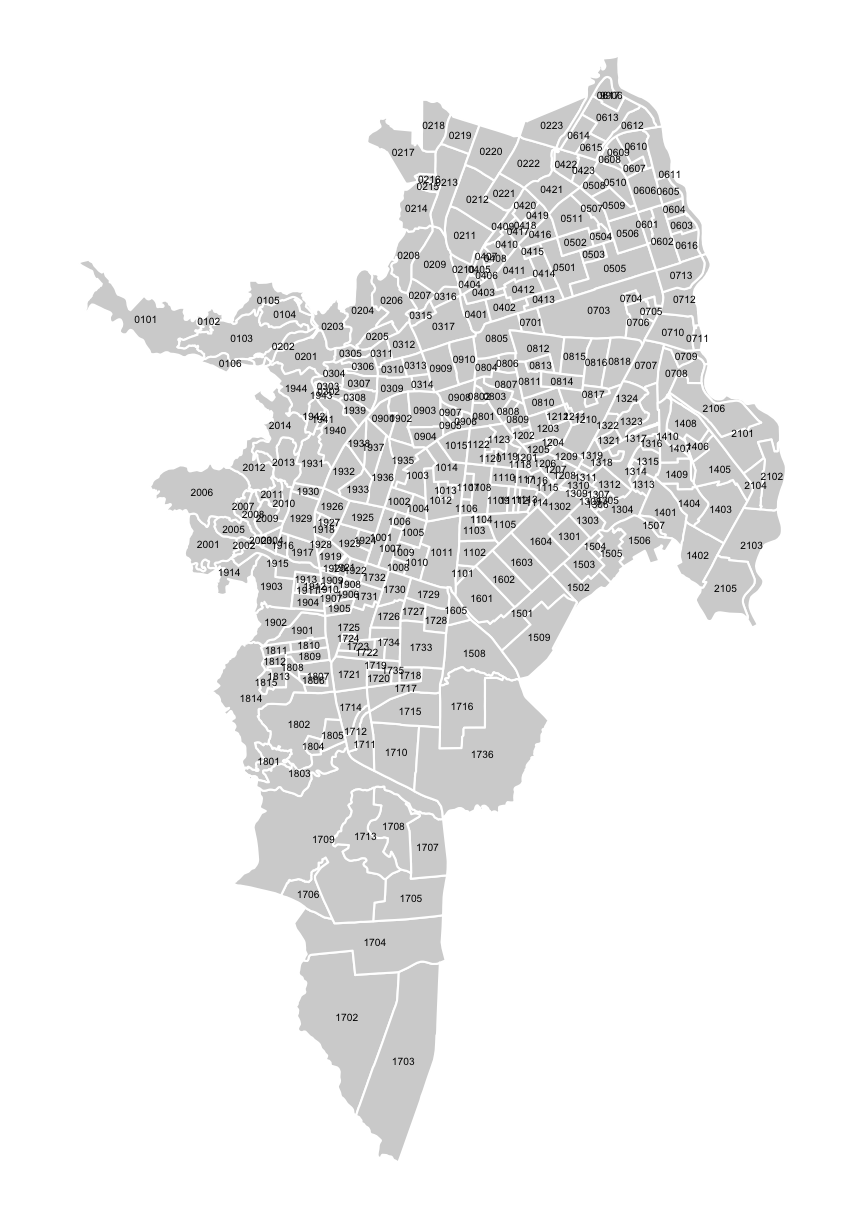
\includegraphics[width=1\linewidth]{tesis-unigis_files/figure-latex/mapa-su-1} \caption{Sectores Urbanos del Censo del 2005. Los sectores seleccionados están parcial o totalmente contenidos en el perímetro urbano 2015}\label{fig:mapa-su}
\end{figure}

La capa de manzanas es necesaria para refinar las capas de espacio verde
y poder calcular el área de calle , área privada y otras métricas sobre
la estructura de cada sector sector censal y que servirán como criterios
para la selección de sectores urbanos a incluir en los análisis de
regresión.

\begin{figure}
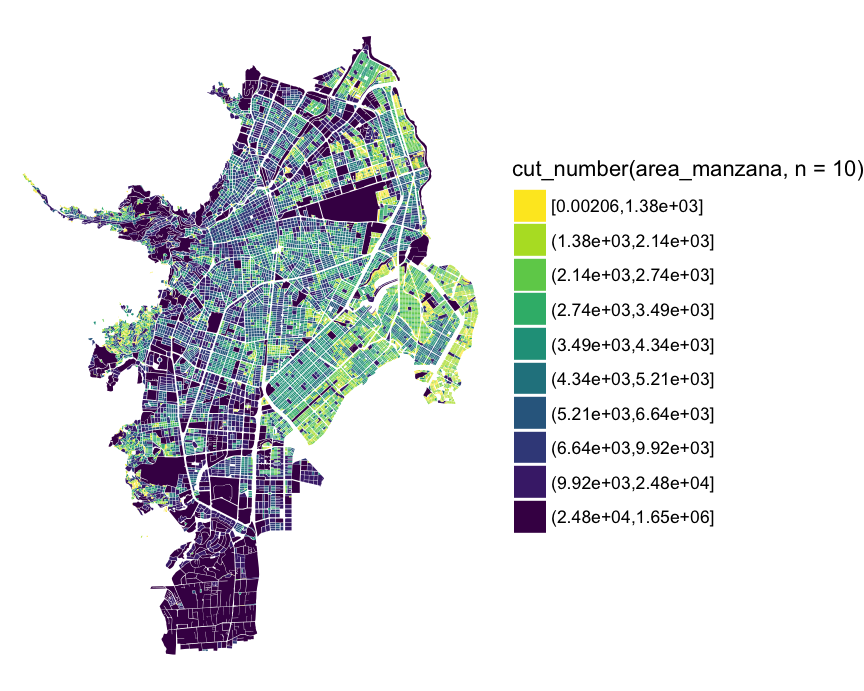
\includegraphics[width=1\linewidth]{tesis-unigis_files/figure-latex/mapa-manzana-1} \caption{Coropleta del tamaño de manzana.Se usaron 10 grupos con aprox. el mismo número de observaciones}\label{fig:mapa-manzana}
\end{figure}

Las capas de equipamiento de la EEC y espacio público se consolidan en
una sola capa conservando la mayor cantidad de información sobre la
clasificación de los tipos de espacios disponibles. El resultado puede
ver verse de forma total (ver figuara \ref{fig:mapa-ev}) o por tipo de
espacio (figuras \ref{fig:mapa-ev-facet} y \ref{fig:mapa-ev-color}).

\begin{figure}
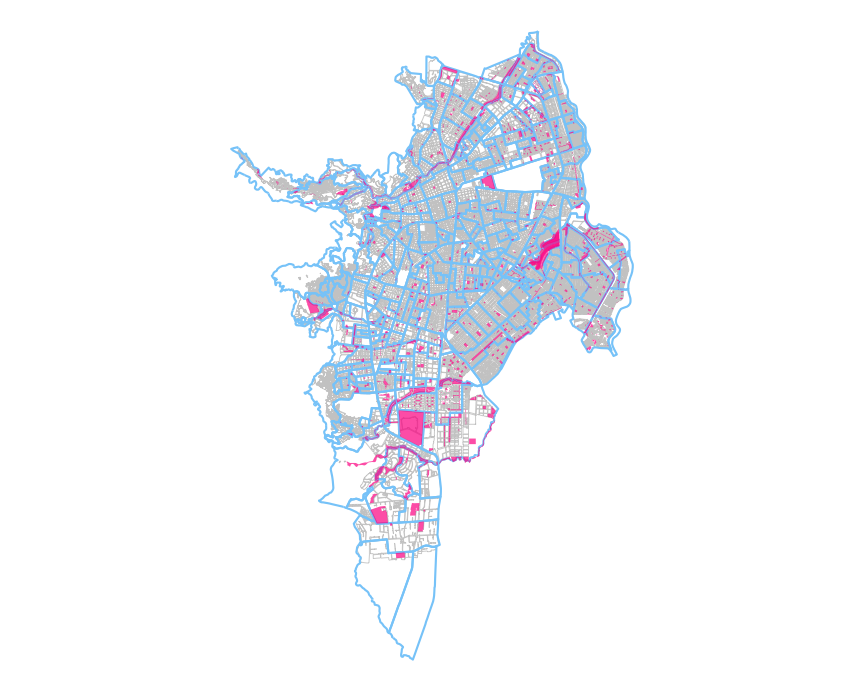
\includegraphics[width=1\linewidth]{tesis-unigis_files/figure-latex/mapa-ev-1} \caption{Espacio verdes consolidados y sectores urbanos}\label{fig:mapa-ev}
\end{figure}

\begin{figure}
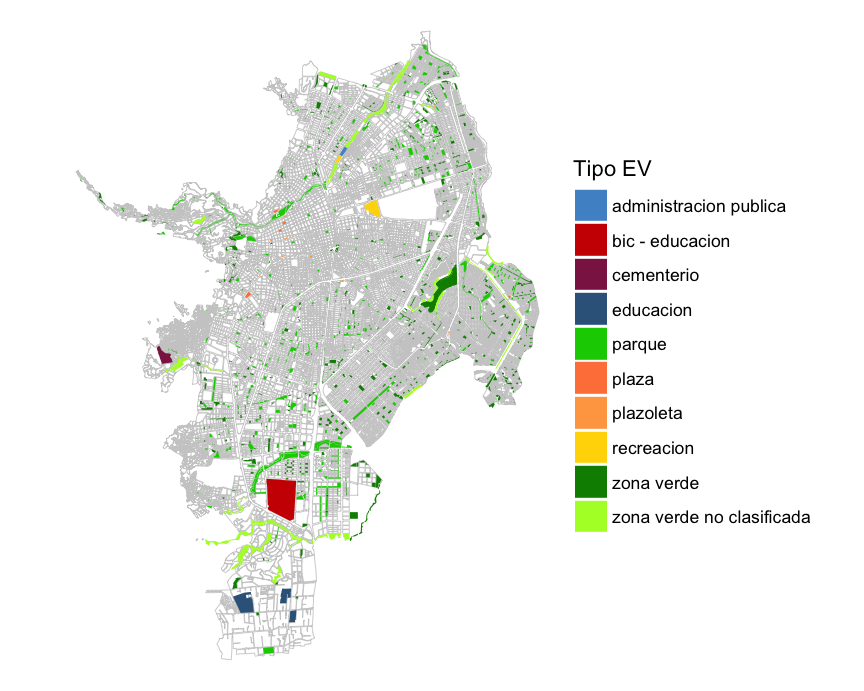
\includegraphics[width=1\linewidth]{tesis-unigis_files/figure-latex/mapa-ev-color-1} \caption{Espacio verde por categoría}\label{fig:mapa-ev-color}
\end{figure}

\begin{figure}
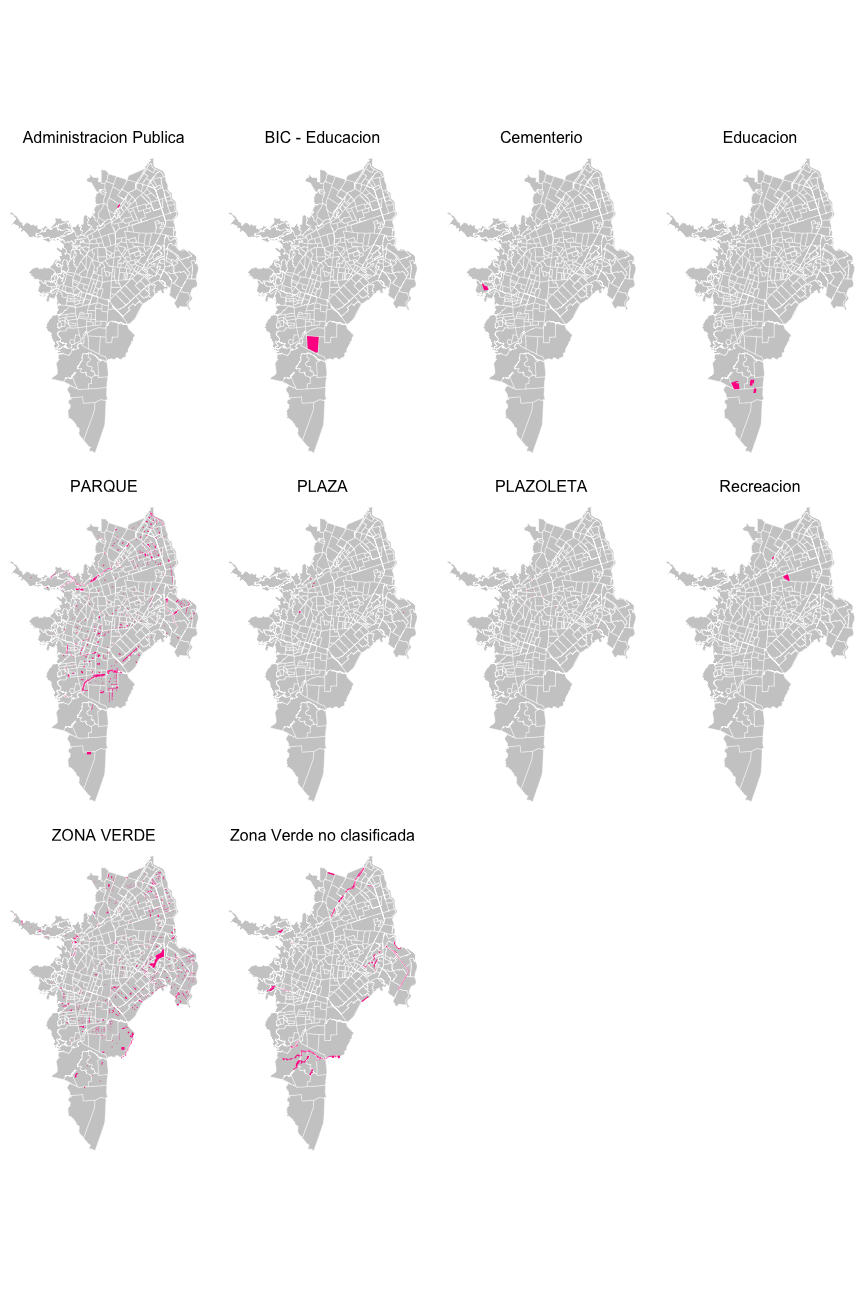
\includegraphics[width=1\linewidth]{tesis-unigis_files/figure-latex/mapa-ev-facet-1} \caption{Small Multiple del espacio verde por categoría}\label{fig:mapa-ev-facet}
\end{figure}

\subsection{Índices de acceso a espacios
verdes}\label{indices-de-acceso-a-espacios-verdes}

Para mejorar la lectura de esta sección se incluyen a continuación las
ecuaciones que definen los índices de acceso seleccionados y las
variantes definidas en este trabajo.

\subsubsection*{Índices de acceso basados en
área}\label{indices-de-acceso-basados-en-area}
\addcontentsline{toc}{subsubsection}{Índices de acceso basados en área}

\textbf{índice contenedor} (area\_ep)

\begin{equation}
A^{C}_i =\sum_j{s_j} \;  \; \forall  j \in I
\label{eq:cont}
\end{equation}

donde \(s_j\) es el área de cada espacio verde \(j\) que pertenece al
conjunto \(I\) de EV dentro del sector \(i\).

\textbf{índice contenedor porcentual} (area\_ep.porcentaje)

\begin{equation}
A^{C_p}_i =1/a_i\sum_j{s_j} \;  \; \forall  j \in I
\label{eq:n-cont}
\end{equation}

donde \(a_i\) es el área del sector \(i\).

\textbf{índice área disponible en radio} (ia.areas.1000)

\begin{equation}
A^{AR}_i= \sum_{\int R_b }{(s_j}  \;  \; \forall  j \in I_{R_b} \; 
\label{eq:area-radio}
\end{equation}

donde \(R_b\) es el radio de búsqueda, \(s_j\) es el área de cada
espacio verde \(j\) que pertenece al conjunto \(I_{R_b}\) de EVs en el
radio de búsqueda.

\textbf{índice porcentual de área disponible en radio}
(ia.areas.1000.porcentaje)

\begin{equation}
A^{AR_p}_i= 1/a_t \sum_{\int R_b }{(s_j}  \;  \; \forall  j \in I_{R_b} \; 
\label{eq:area-radio2}
\end{equation}

donde \(a_t\) es el área total de espacio verde en la ciudad.

\subsubsection*{Índices de acceso basados en
distancia}\label{indices-de-acceso-basados-en-distancia}
\addcontentsline{toc}{subsubsection}{Índices de acceso basados en
distancia}

\textbf{costo de viaje} (ia.costoviaje)

\begin{equation}
A^{T}_i =\sum_j{d_{ij}} \; \; \forall  j \in I_t
\label{eq:costo}
\end{equation}

donde \(d_{ij}\) es la distancia del centriode del sector \(i\) al
espacio \(j\) e \(I_t\) es el conjunto de todos los epacios verdes de la
ciudad.

\textbf{costo de viaje normalizado} (ia.costo.n)

\begin{equation}
\bar{A}^{T_n}_i =A^{T}_i/N 
\label{eq:n-costo}
\end{equation}

donde \(N\) es el número total de espacio verdes en la ciudad.

\textbf{distancia mínima} (ia.mindist)

\begin{equation}
A^{M}_i=min\left | d_{ij} \right | \forall  j \in I_t
\label{eq:min-dist}
\end{equation}

\subsubsection*{Índices de acceso
mixtos}\label{indices-de-acceso-mixtos}
\addcontentsline{toc}{subsubsection}{Índices de acceso mixtos}

\textbf{razón área distancia} (ia.A.D)

\begin{equation}
A^{AD}_i= \sum_{\int R_b }{s_j/d_{ij}}  \;  \; \forall  j \in I_{R_b} \; 
\label{eq:area-dist}
\end{equation}

donde \(R_b\) es el radio de búsqueda, \(s_j\) es el área de cada
espacio verde \(j\), \(d_{ij}\) es la distancia del centriode del sector
\(i\) al espacio \(j\) que pertenecen al conjunto \(I_{R_b}\) de EVs en
el radio de búsqueda.

\textbf{razón área disponible distancia} (ia.areas.dist)

\begin{equation}
\bar{A}^{AD}_i= \frac{\sum_{\int R_b }{s_j}}{\sum_{\int R_b }{d_{ij}}}  \;  \; \forall  j \in I_{R_b} \; 
\label{eq:areas-dists}
\end{equation}

Con los datos consolidados se calculan las áreas de los espacios verdes
al interior de cada sector censal, para calcular los índices de acceso
tipo contenedor (ecuación \eqref{eq:cont}) interceptando los espacio
verdes con los sectores urbanos (ecuación \eqref{eq:n-cont}). También se
obtuvo una versión del índice contenedor como en porcentaje del área del
SU. El cálculo de los índices de costo de viajes (ecuación
\eqref{eq:costo}) y costo de viaje normalizado (ecuación \eqref{eq:n-costo})
se obtiene creado una matriz de distancia entre los centroides de los
sectores censales y cada uno de los espacios verdes. De esta matriz de
distancia también se obtiene el índice de distancia mínima (ecuación
\eqref{eq:min-dist}).

Los mapas de los índices de acceso basados en distancia se muestran en
la figura \ref{fig:mapas-ia-distancia}

\begin{figure}
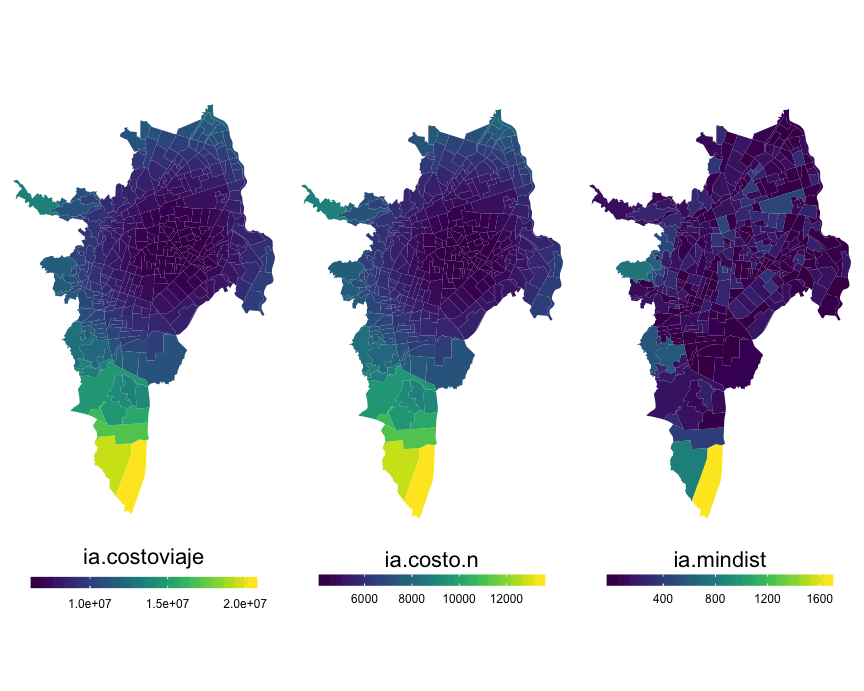
\includegraphics[width=1\linewidth]{tesis-unigis_files/figure-latex/mapas-ia-distancia-1} \caption{Small Multiple de los indices de acceso a EV basados en distancia en escala continua}\label{fig:mapas-ia-distancia}
\end{figure}

\begin{figure}
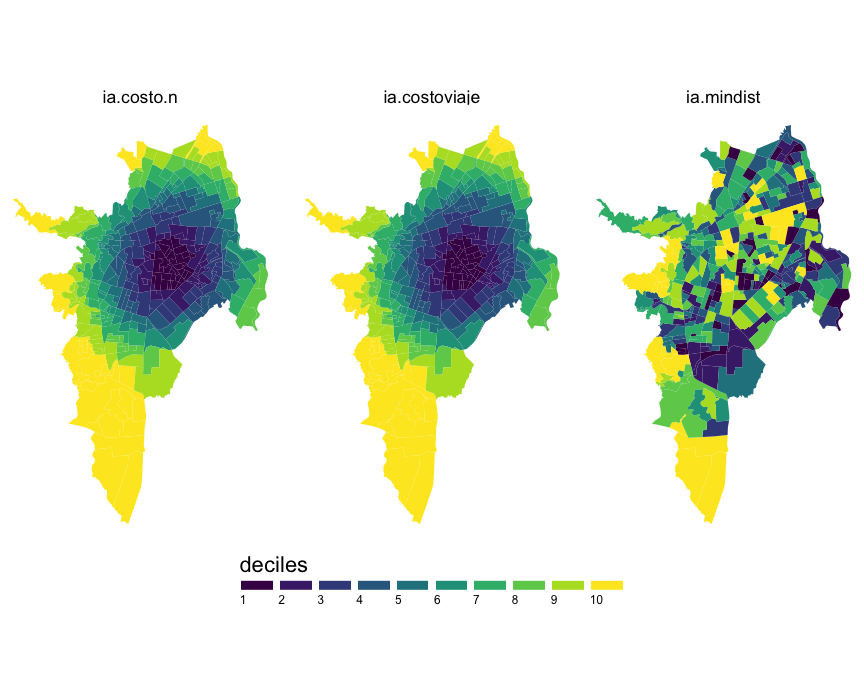
\includegraphics[width=1\linewidth]{tesis-unigis_files/figure-latex/mapas-ia-distancia-deciles-1} \caption{Small Multiple de los indices de acceso a EV basados en distancia usando deciles}\label{fig:mapas-ia-distancia-deciles}
\end{figure}

Además de los índices basados en distancia y el tipo contenedor se
calcularon índices de acceso basados en el área de espacio verde en un
radio de 1000 metros. Estos índices muestran un dimensión relacionada no
con solo con el acceso sino con la cantidad de espacio disponible en el
radio de busqueda definido desde el centroide del sector censal. Para
hacernos una idea del radio de búsqueda seleccionado, el siguiente mapa
muestra los radios búsqueda y los espacios verdes.

\begin{figure}
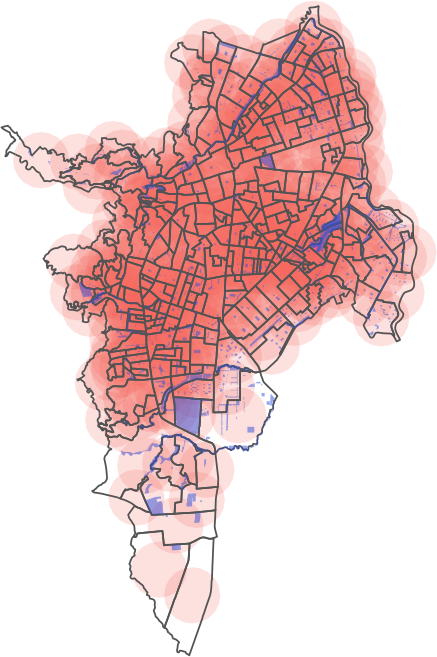
\includegraphics[width=1\linewidth]{tesis-unigis_files/figure-latex/mapa-rango1km-1} \caption{Espacio verdes y rango de 1 km desde centriodes de SU}\label{fig:mapa-rango1km}
\end{figure}

Los índices de acceso basados en área descritos en las ecuaciones
\eqref{eq:cont},\eqref{eq:n-cont} y\eqref{eq:area-radio} se resumen en la
siguiente gráfica.

\begin{figure}
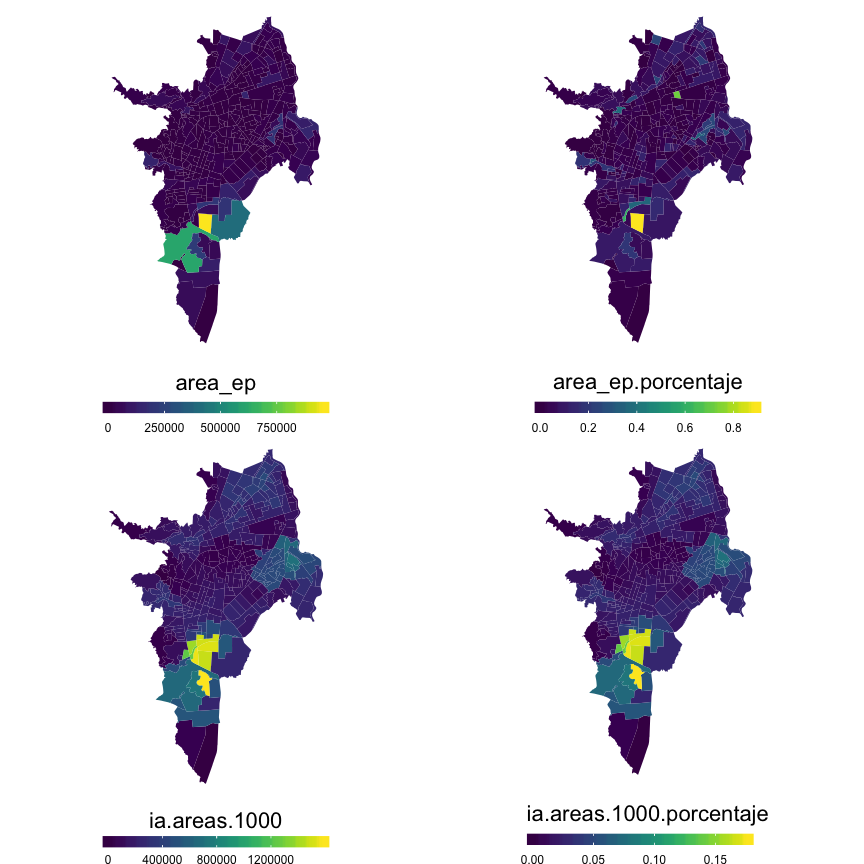
\includegraphics[width=1\linewidth]{tesis-unigis_files/figure-latex/mapas-ia-area-1} \caption{Small Multiple de los indices de acceso a EV basados en área usando escala continua}\label{fig:mapas-ia-area}
\end{figure}

\begin{figure}
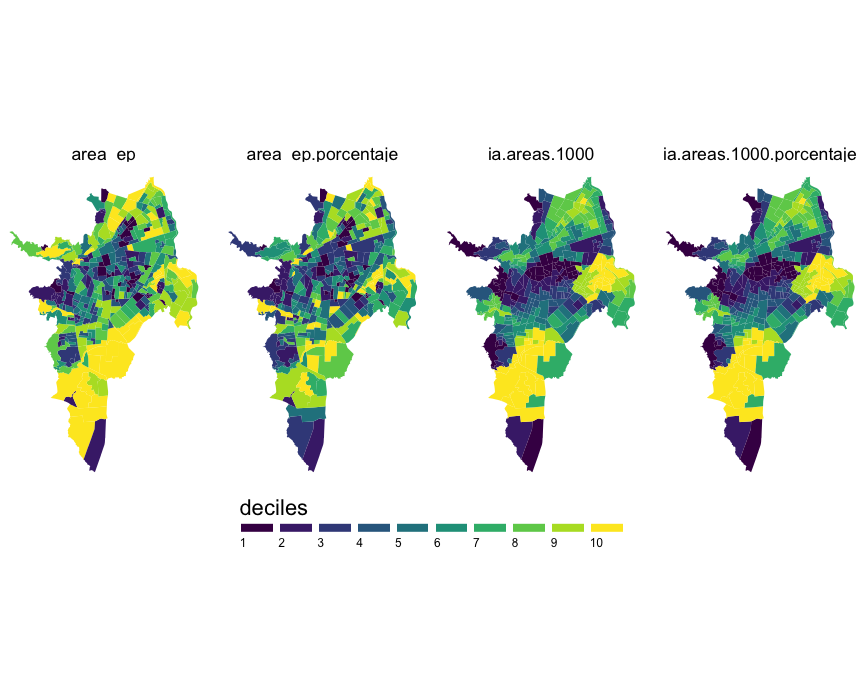
\includegraphics[width=1\linewidth]{tesis-unigis_files/figure-latex/mapas-ia-area-deciles-1} \caption{Small Multiple de los indices de acceso a EV basados en distancia usando deciles}\label{fig:mapas-ia-area-deciles}
\end{figure}

En la búsqueda de índices de acceso más complejos que reflejen el acceso
en distancia y la cantidad de área disponible desde cada sector urbano
se construyeron índices similares a el índice de distancia de a pie
(ecuación \eqref{eq:walkdist} que se basan en la razón entre el área a la
que se accede y la distancia a la que se encuentra del centroide del
sector. Dos nuevos índices se proponen en este trabajo: ia.areas.dist
(ecuación \eqref{eq:areas-dists}) como la suma de las áreas en el rango de
1 km desde el centroide del SU dividido la suma de las distancia a esos
EV; ia.A.D (ecuación \eqref{eq:area-dist}) , que es la suma de las razones
entre el área del espacio verde \(j\) dividido entre la distancia
\(d_{ij}\) desde el centroide del SU \(i\) al EV \(j\). La siguiente
gráfica muestra las métricas propuestas.

\begin{figure}
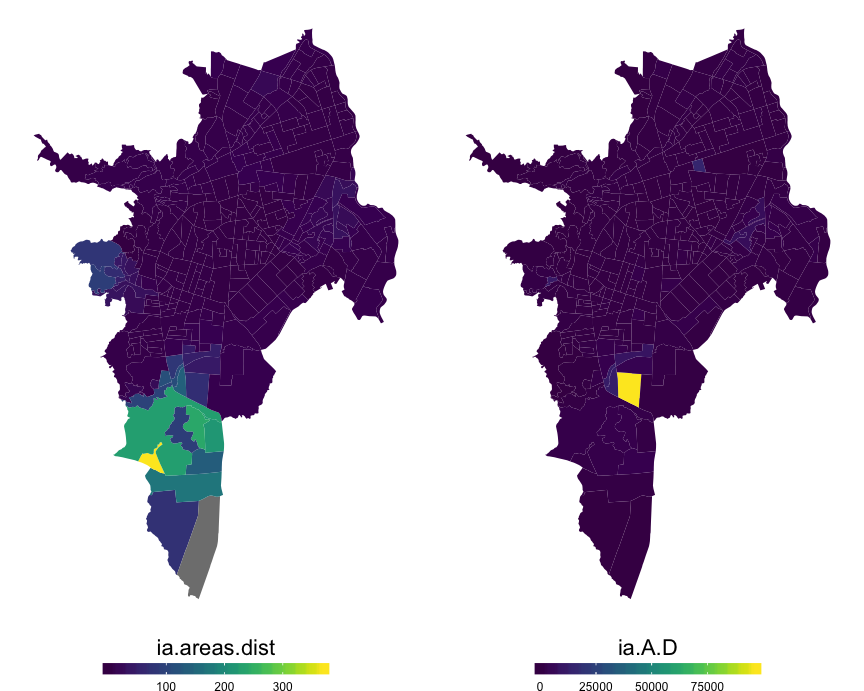
\includegraphics[width=1\linewidth]{tesis-unigis_files/figure-latex/mapas-ia-area-dist-1} \caption{Small Multiple de los indices de acceso a EV basados en área y distancia usando escala continua}\label{fig:mapas-ia-area-dist}
\end{figure}

\begin{figure}
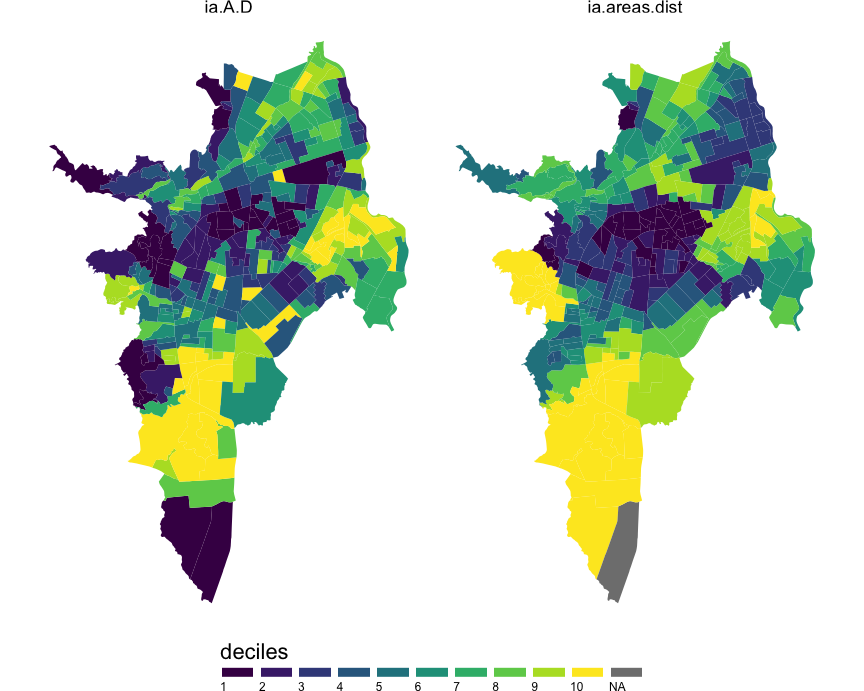
\includegraphics[width=1\linewidth]{tesis-unigis_files/figure-latex/mapas-ia-area-dist-deciles-1} \caption{Small Multiple de los indices de acceso a EV basados en distancia usando deciles}\label{fig:mapas-ia-area-dist-deciles}
\end{figure}

Además de los mapas es de interes observar la distribución en frecuencia
de las métricas de acceso. La siguiente gráfica se observan los
histogramas de las metricas calculadas.

\begin{figure}
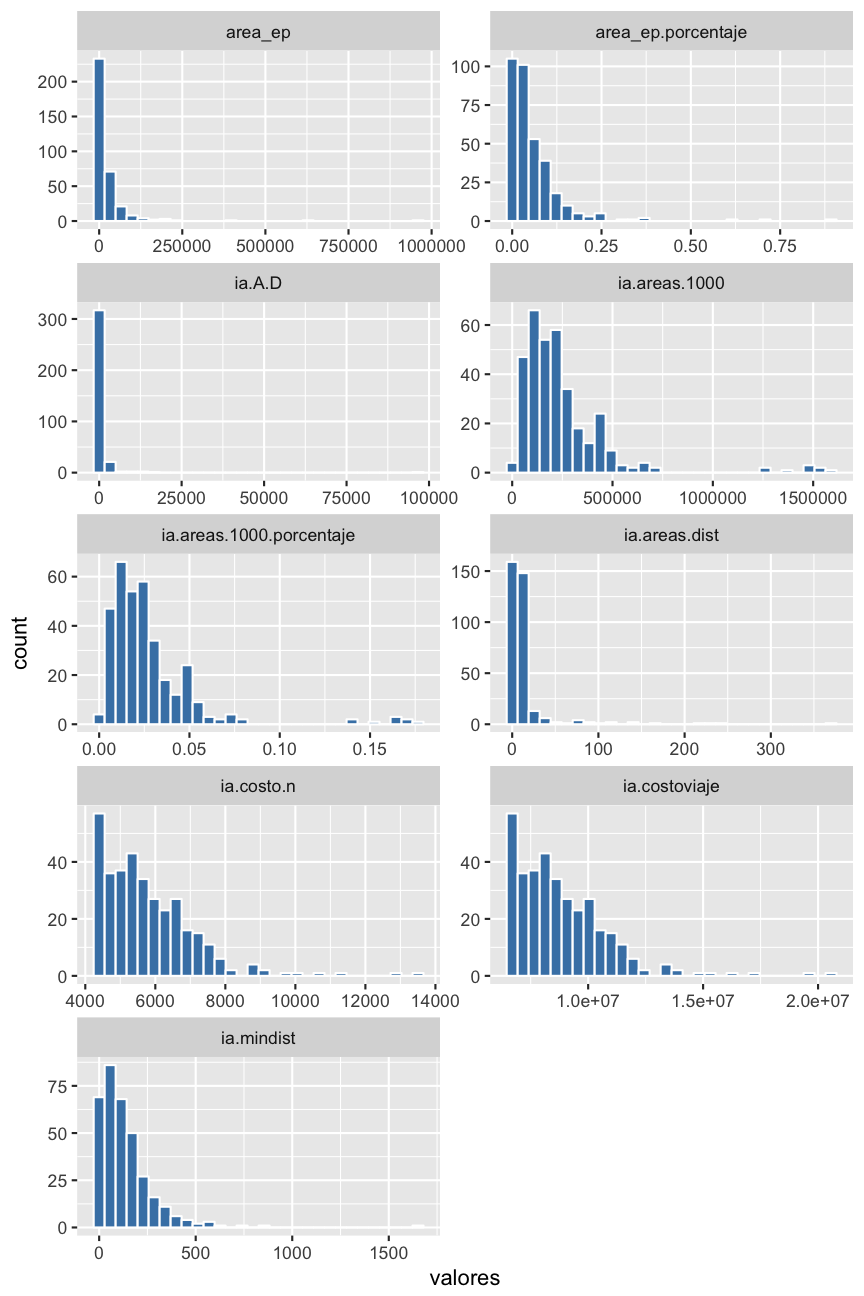
\includegraphics[width=1\linewidth]{tesis-unigis_files/figure-latex/hist-acceso-1} \caption{Small Multiple de los indices de acceso a EV basados en distancia usando deciles}\label{fig:hist-acceso}
\end{figure}

Finalmente se muestra el código en R que calcula los índices
presentados, y el resumen de los índices calculados.

\begin{verbatim}
##  ia.costoviaje        ia.costo.n      ia.mindist         area_ep      
##  Min.   : 6538022   Min.   : 4293   Min.   :  10.00   Min.   :     0  
##  1st Qu.: 7299897   1st Qu.: 4793   1st Qu.:  35.94   1st Qu.:  2158  
##  Median : 8376735   Median : 5500   Median :  95.58   Median :  7710  
##  Mean   : 8789929   Mean   : 5771   Mean   : 135.94   Mean   : 25712  
##  3rd Qu.: 9836587   3rd Qu.: 6459   3rd Qu.: 178.27   3rd Qu.: 25288  
##  Max.   :20407619   Max.   :13400   Max.   :1661.44   Max.   :959105  
##                                                                       
##  area_ep.porcentaje ia.areas.1000     ia.areas.1000.porcentaje
##  Min.   :0.00000    Min.   :      0   Min.   :0.00000         
##  1st Qu.:0.00964    1st Qu.: 117574   1st Qu.:0.01306         
##  Median :0.03410    Median : 193016   Median :0.02145         
##  Mean   :0.05866    Mean   : 249755   Mean   :0.02775         
##  3rd Qu.:0.07671    3rd Qu.: 292520   3rd Qu.:0.03250         
##  Max.   :0.89245    Max.   :1589082   Max.   :0.17657         
##                                                               
##  ia.areas.dist          ia.A.D       
##  Min.   :  0.4185   Min.   :    0.0  
##  1st Qu.:  3.9850   1st Qu.:  240.8  
##  Median :  6.7780   Median :  434.4  
##  Mean   : 15.1800   Mean   : 1119.4  
##  3rd Qu.: 11.4793   3rd Qu.:  849.7  
##  Max.   :370.2725   Max.   :96664.6  
##  NA's   :1
\end{verbatim}

\begin{Shaded}
\begin{Highlighting}[]
\CommentTok{# matriz distancia entre centriodes y espacios}
\NormalTok{m.dist.ctrdsu.ep <-}\StringTok{ }\KeywordTok{gDistance}\NormalTok{(ep.cali, centroides.su, }\DataTypeTok{byid =}\NormalTok{ T)}
\CommentTok{# cuando el punto esta dentro del poligono el valor que rertorna es 0 por}
\CommentTok{# ese motivo le pondremos 10 a valores = 0 o entre 0 y 10 para evitar}
\CommentTok{# problemas al invertir la matriz y mejorar la conistencia del indices con}
\CommentTok{# valores inversos a la distancia}
\NormalTok{m.dist.ctrdsu.ep[m.dist.ctrdsu.ep }\OperatorTok{<}\StringTok{ }\DecValTok{10}\NormalTok{] <-}\StringTok{ }\DecValTok{10}
\CommentTok{# matriz consicion de estar a 1000 del centriodo}
\NormalTok{is.}\FloatTok{1000.}\NormalTok{ep <-}\StringTok{ }\KeywordTok{gWithinDistance}\NormalTok{(ep.cali, centroides.su, }\DecValTok{1001}\NormalTok{, }\DataTypeTok{byid =}\NormalTok{ T)}
\CommentTok{# cantidad de espacio verdes en radio de 1000 m de los centriodes del sector}
\CommentTok{# urbano}
\NormalTok{num.ep.}\DecValTok{1000}\NormalTok{ <-}\StringTok{ }\KeywordTok{apply}\NormalTok{(is.}\FloatTok{1000.}\NormalTok{ep, }\DecValTok{1}\NormalTok{, }\ControlFlowTok{function}\NormalTok{(x) }\KeywordTok{sum}\NormalTok{(x, }\DataTypeTok{na.rm =}\NormalTok{ T))}
\CommentTok{# distancias de Espacio publicos a 1000 del centriode de SU}
\NormalTok{a <-}\StringTok{ }\NormalTok{m.dist.ctrdsu.ep }\OperatorTok{*}\StringTok{ }\NormalTok{is.}\FloatTok{1000.}\NormalTok{ep}

\CommentTok{# distancia minima distinta de 0}
\NormalTok{ia.mindist <-}\StringTok{ }\KeywordTok{apply}\NormalTok{(m.dist.ctrdsu.ep, }\DecValTok{1}\NormalTok{, }\ControlFlowTok{function}\NormalTok{(x) }\KeywordTok{min}\NormalTok{(x[x }\OperatorTok{!=}\StringTok{ }\DecValTok{0}\NormalTok{]))}
\NormalTok{index.min <-}\StringTok{ }\KeywordTok{apply}\NormalTok{(m.dist.ctrdsu.ep, }\DecValTok{1}\NormalTok{, }\ControlFlowTok{function}\NormalTok{(x) }\KeywordTok{which.min}\NormalTok{(x[x }\OperatorTok{!=}\StringTok{ }\DecValTok{0}\NormalTok{]))}
\NormalTok{ia.area.mindist <-}\StringTok{ }\NormalTok{ep.cali}\OperatorTok{$}\NormalTok{area_ep[index.min]}\OperatorTok{/}\NormalTok{ia.mindist}
\CommentTok{# suma de las distancias a cada EP por centriode}
\NormalTok{ia.costoviaje <-}\StringTok{ }\KeywordTok{apply}\NormalTok{(m.dist.ctrdsu.ep, }\DecValTok{1}\NormalTok{, sum)}
\CommentTok{# suma de las distancias a cada EP ubicado a menos de 1000 m del centriode}
\NormalTok{ia.}\DecValTok{1000}\NormalTok{ <-}\StringTok{ }\KeywordTok{apply}\NormalTok{(a, }\DecValTok{1}\NormalTok{, }\ControlFlowTok{function}\NormalTok{(x) }\KeywordTok{sum}\NormalTok{(x))}
\NormalTok{ia.}\DecValTok{1000}\NormalTok{[ia.}\DecValTok{1000} \OperatorTok{==}\StringTok{ }\DecValTok{0}\NormalTok{] <-}\StringTok{ }\OtherTok{NA}
\NormalTok{ia.}\FloatTok{1000.}\NormalTok{n <-}\StringTok{ }\NormalTok{ia.}\DecValTok{1000}\OperatorTok{/}\NormalTok{num.ep.}\DecValTok{1000}
\CommentTok{# indice de la suma de las areas en el rango de un 1 km del sector censal}
\NormalTok{ia.areas.}\DecValTok{1000}\NormalTok{ <-}\StringTok{ }\NormalTok{is.}\FloatTok{1000.}\NormalTok{ep }\OperatorTok\StringTok{ }\NormalTok{ep.cali}\OperatorTok{$}\NormalTok{area_ep }\OperatorTok\StringTok{ }\KeywordTok{as.vector}\NormalTok{()}
\CommentTok{# indice de area disponible en el radio de 1km como porcentaje del area}
\CommentTok{# total disponible}

\NormalTok{ia.areas.}\FloatTok{1000.}\NormalTok{porcentaje <-}\StringTok{ }\NormalTok{ia.areas.}\DecValTok{1000}\OperatorTok{/}\KeywordTok{sum}\NormalTok{(ep.cali}\OperatorTok{$}\NormalTok{area_ep)}

\CommentTok{# matriz de distancias inversas de centriode su a espacios verdes}
\NormalTok{m.dist.ctrdsu.}\FloatTok{1000.}\NormalTok{ep.inv <-}\StringTok{ }\DecValTok{1}\OperatorTok{/}\NormalTok{a}
\NormalTok{b <-}\StringTok{ }\NormalTok{m.dist.ctrdsu.}\FloatTok{1000.}\NormalTok{ep.inv }\OperatorTok{*}\StringTok{ }\KeywordTok{is.finite}\NormalTok{(m.dist.ctrdsu.}\FloatTok{1000.}\NormalTok{ep.inv)  }\CommentTok{# eliminar infinitos}
\CommentTok{# suma de inverso de las distancias a cada EP ubicado a menos de 1000 m del}
\CommentTok{# centriode}
\NormalTok{ia.}\FloatTok{1000.}\NormalTok{inv <-}\StringTok{ }\KeywordTok{apply}\NormalTok{(b, }\DecValTok{1}\NormalTok{, }\ControlFlowTok{function}\NormalTok{(x) }\KeywordTok{sum}\NormalTok{(x, }\DataTypeTok{na.rm =}\NormalTok{ T))}
\NormalTok{ia.}\FloatTok{1000.}\NormalTok{inv[ia.}\FloatTok{1000.}\NormalTok{inv }\OperatorTok{==}\StringTok{ }\DecValTok{0}\NormalTok{] <-}\StringTok{ }\OtherTok{NA}
\CommentTok{# razon entre Area del EP y distancia al centriode}
\NormalTok{A.D <-}\StringTok{ }\KeywordTok{t}\NormalTok{(}\KeywordTok{t}\NormalTok{(b) }\OperatorTok{*}\StringTok{ }\NormalTok{ep.cali}\OperatorTok{$}\NormalTok{area_ep)}

\CommentTok{# sumatoria de la razon entre Area del EP y distancias de ese EP al}
\CommentTok{# centriode}
\NormalTok{ia.A.D <-}\StringTok{ }\KeywordTok{apply}\NormalTok{(A.D, }\DecValTok{1}\NormalTok{, }\ControlFlowTok{function}\NormalTok{(x) }\KeywordTok{sum}\NormalTok{(x, }\DataTypeTok{na.rm =}\NormalTok{ T))}
\KeywordTok{class}\NormalTok{(ia.costoviaje)}
\KeywordTok{summary}\NormalTok{(ia.costoviaje)}
\KeywordTok{length}\NormalTok{(ia.costoviaje)}
\KeywordTok{summary}\NormalTok{(ia.}\FloatTok{1000.}\NormalTok{inv)}
\KeywordTok{length}\NormalTok{(ia.A.D)}
\KeywordTok{summary}\NormalTok{(ia.A.D)}

\CommentTok{# consolidadcionde indices calculados}
\NormalTok{ia.ev <-}\StringTok{ }\KeywordTok{data.frame}\NormalTok{(su}\OperatorTok{$}\NormalTok{SETU_CCDGO, ia.costoviaje)}
\NormalTok{ia.ev}\OperatorTok{$}\NormalTok{ia.costo.n <-}\StringTok{ }\NormalTok{ia.ev}\OperatorTok{$}\NormalTok{ia.costoviaje}\OperatorTok{/}\KeywordTok{dim}\NormalTok{(m.dist.ctrdsu.ep)[}\DecValTok{2}\NormalTok{]}
\NormalTok{ia.ev <-}\StringTok{ }\KeywordTok{bind_cols}\NormalTok{(ia.ev, }\KeywordTok{data.frame}\NormalTok{(ia.}\DecValTok{1000}\NormalTok{, ia.}\FloatTok{1000.}\NormalTok{inv, ia.}\FloatTok{1000.}\NormalTok{n, ia.areas.}\DecValTok{1000}\NormalTok{, }
\NormalTok{    ia.areas.}\FloatTok{1000.}\NormalTok{porcentaje))}
\NormalTok{ia.ev}\OperatorTok{$}\NormalTok{ia.r300 <-}\StringTok{ }\DecValTok{300} \OperatorTok{*}\StringTok{ }\NormalTok{ia.}\FloatTok{1000.}\NormalTok{inv}
\NormalTok{ia.ev <-}\StringTok{ }\NormalTok{ia.ev }\OperatorTok\StringTok{ }\NormalTok{dplyr}\OperatorTok{::}\KeywordTok{rename}\NormalTok{(}\DataTypeTok{SETU_CCDGO =}\NormalTok{ su.SETU_CCDGO)}
\NormalTok{ia.ev}\OperatorTok{$}\NormalTok{ia.mindist <-}\StringTok{ }\NormalTok{ia.mindist}
\NormalTok{ia.ev}\OperatorTok{$}\NormalTok{ia.area.mindist <-}\StringTok{ }\NormalTok{ia.area.mindist}
\NormalTok{ia.ev}\OperatorTok{$}\NormalTok{ia.A.D <-}\StringTok{ }\NormalTok{ia.A.D}
\NormalTok{smry.area <-}\StringTok{ }\KeywordTok{summary}\NormalTok{(ep.cali}\OperatorTok{$}\NormalTok{area_ep)}
\NormalTok{ia.ev}\OperatorTok{$}\NormalTok{ia.r300.Amedia <-}\StringTok{ }\DecValTok{300}\OperatorTok{/}\NormalTok{smry.area[}\DecValTok{4}\NormalTok{] }\OperatorTok{*}\StringTok{ }\NormalTok{ia.ev}\OperatorTok{$}\NormalTok{ia.A.D}
\NormalTok{ia.ev}\OperatorTok{$}\NormalTok{ia.r300.Amediana <-}\StringTok{ }\DecValTok{300}\OperatorTok{/}\NormalTok{smry.area[}\DecValTok{3}\NormalTok{] }\OperatorTok{*}\StringTok{ }\NormalTok{ia.ev}\OperatorTok{$}\NormalTok{ia.A.D}
\NormalTok{ia.ev}\OperatorTok{$}\NormalTok{ia.areas.dist <-}\StringTok{ }\NormalTok{ia.areas.}\DecValTok{1000}\OperatorTok{/}\NormalTok{ia.}\DecValTok{1000}
\end{Highlighting}
\end{Shaded}

\section{Datos del censo arbóreo 2015}\label{sec-ca2015}

El censo arbóreo del año 2015 consolidó un inventario de la vegetación
de la ciudad compuesto por 296438 individuos. Entre las variables que
categorizan los individuos censados están el tipo de emplazamiento, tipo
de suelo que cubre la vegetación, la edad, la vitalidad, tipo de
vegetación y sus caratetiristicas dasometricas p.ej la altura, el
diamtro de la copa, altura y diametro del pecho, etc \ldots{}, entro
otras relacionadas con el estado fitosanitario y daños físicos.

A continuación se presentan una serie de tablas que resumen las
caraterísticas seleccionadas en la tabla \ref{tab:vars-AU} para el
análisis (por tipo de vegetación \ref{tab:ca2015-vegetacion}, por edad
\ref{tab:ca2015-edad} y por emplazamiento
\ref{tab:ca2015-emplazamiento}), antes de aplicar los criterios de
seleccón de los individuos arbóres para este estudio.

\begin{table}

\caption{\label{tab:ca2015-vegetacion}Resúmen CA2015 por tipo de vegetación}
\centering
\begin{tabular}[t]{l|r|r|r}
\hline
Tipo de vegetación & altura media & diámetro medio & cantidad\\
\hline
Arbol & 7.32 & 7.14 & 200528\\
\hline
Arbusto & 3.34 & 2.91 & 42872\\
\hline
Bambu & 11.73 & 3.34 & 419\\
\hline
Muerto & 2.30 & 1.00 & 1\\
\hline
Palma & 5.53 & 3.93 & 49777\\
\hline
Planta arbustiva & 2.77 & 2.83 & 2176\\
\hline
Seco & 5.79 & 3.63 & 665\\
\hline
\end{tabular}
\end{table}

\begin{table}

\caption{\label{tab:ca2015-edad}Resúmen CA2015 por edad}
\centering
\begin{tabular}[t]{l|r|r|r}
\hline
Edad & altura media & diámetro medio & cantidad\\
\hline
Juvenil & 3.63 & 3.10 & 49473\\
\hline
Maduro & 6.60 & 6.11 & 214042\\
\hline
Longevo & 9.39 & 9.16 & 32923\\
\hline
\end{tabular}
\end{table}

\begin{table}

\caption{\label{tab:ca2015-emplazamiento}Resúmen CA2015 por emplazamiento}
\centering
\begin{tabular}[t]{l|r|r|r}
\hline
Emplazamiento & altura media & diámetro medio & cantidad\\
\hline
Anden & 5.96 & 5.49 & 136948\\
\hline
Bahias de estacionamiento & 6.61 & 6.23 & 1927\\
\hline
Bulevares & 4.30 & 3.03 & 85\\
\hline
Corredor Ferreo & 6.99 & 7.22 & 1534\\
\hline
Escenario deportivo y/o Cultural & 7.14 & 6.47 & 32757\\
\hline
Glorieta & 6.01 & 5.69 & 777\\
\hline
Parque Urbano & 6.83 & 6.29 & 56137\\
\hline
Paseos & 5.81 & 5.34 & 2573\\
\hline
Plaza & 7.50 & 6.63 & 65\\
\hline
Plazoleta & 6.92 & 5.80 & 1773\\
\hline
Ronda de rios & 8.21 & 7.15 & 7424\\
\hline
Rondas de canales & 6.13 & 5.88 & 11721\\
\hline
Separador Vial & 6.51 & 6.32 & 42717\\
\hline
\end{tabular}
\end{table}

Existe una diferencia de 10 años entre censo de población de 2005 y el
censo arbóreo de la ciudad de Cali. Aunque esto pueda parecer una
situación que reduce la legitimidad de los resultados que se hayen en
este estudio, autores como \citet{boone2010landscape} y
\citet{schwarz_trees_2015} reconocen que los paisajes que vemos hoy son
legados de patrones de consumo pasados, y que en el caso de la
vegetación urbana tratamos con organismos de larga vida que pueden
tardar mucho tiempo en establecerse y crecer. En contraste, la
estructura social de las ciudades puede cambiar más rápidamente.

Como se menciona en la metodología, la apuesta para reducir la brecha es
la exclusión de los árboles jóvenes del inventario, que posiblemente no
estaban ahí en 2005. Aunque no conocemos las tasa anual de tala de
árboles en la ciudad, y dado es posible que una parte importante de los
árboles jóvenes haya reemplazado a los los que fueron talados, no parece
realista mantener el inventario entero.

Aunque en general toda la vegetación aporta beneficios ambientales a los
habitantes, en este estudio descartamos la vegetación arbustiva y los
árboles, palmas y bambú de menos de 1.9 m de altura para
circunscribirnos a los individuos más desarrollados.

Una vez aplicado este filtro contamos con 203112 individuos. Las tablas
de resumen para la selección de indivuduos con base en estos criterios
se muestran a contiunuación.

\begin{table}

\caption{\label{tab:ca2015sel-vegetacion}Resúmen selección CA2015 por tipo de vegetación}
\centering
\begin{tabular}[t]{l|r|r|r}
\hline
Tipo de vegetación & altura media & diámetro medio & cantidad\\
\hline
Arbol & 8.00 & 7.90 & 168133\\
\hline
Bambu & 9.79 & 4.25 & 235\\
\hline
Palma & 6.51 & 4.48 & 34357\\
\hline
Seco & 6.61 & 5.67 & 387\\
\hline
\end{tabular}
\end{table}

\begin{table}

\caption{\label{tab:ca2015sel-edad}Resúmen selección CA2015 por edad}
\centering
\begin{tabular}[t]{l|r|r|r}
\hline
Edad & altura media & diámetro medio & cantidad\\
\hline
Maduro & 7.38 & 6.90 & 172776\\
\hline
Longevo & 9.85 & 9.67 & 30336\\
\hline
\end{tabular}
\end{table}

\begin{table}

\caption{\label{tab:ca2015sel-emplazamiento}Resúmen selección CA2015 por emplazamiento}
\centering
\begin{tabular}[t]{l|r|r|r}
\hline
Emplazamiento & altura media & diámetro medio & cantidad\\
\hline
Anden & 7.25 & 6.82 & 92198\\
\hline
Bahias de estacionamiento & 8.04 & 7.66 & 1348\\
\hline
Bulevares & 8.74 & 8.11 & 17\\
\hline
Corredor Ferreo & 8.56 & 9.03 & 1060\\
\hline
Escenario deportivo y/o Cultural & 8.25 & 7.55 & 24861\\
\hline
Glorieta & 7.29 & 7.06 & 496\\
\hline
Parque Urbano & 8.35 & 7.81 & 37756\\
\hline
Paseos & 7.42 & 7.02 & 1623\\
\hline
Plaza & 9.07 & 7.83 & 49\\
\hline
Plazoleta & 8.47 & 7.00 & 1206\\
\hline
Ronda de rios & 9.18 & 8.25 & 5759\\
\hline
Rondas de canales & 7.41 & 7.23 & 7815\\
\hline
Separador Vial & 7.89 & 7.82 & 28924\\
\hline
\end{tabular}
\end{table}

Para indagar sobre la distribución de estos individuos y no quedarnos
con los resúmenes estadísticos se muestran a continuación los datos
desagregados gráficamente cada una de las variables categóricas y las
características físicas del arbolado: altura, diámetro de la copa y su
ubicación en la ciudad.

En primer lugar indagamos sobre las diferencias de diámetro y altura por
tipo de vegetación. La figura \ref{fig:au-veg} muestra claramente las
diferencias físicas entre los árboles (desarrollan mayor tamaño y con
mayor número de individuos), el bambú y las palmas (más altos que anchos
y en menor número) de la ciudad. Los árboles catalogados como secos,
hace 10 años estaban vivos y los mantenemos en la selección de
individuos.

\begin{figure}
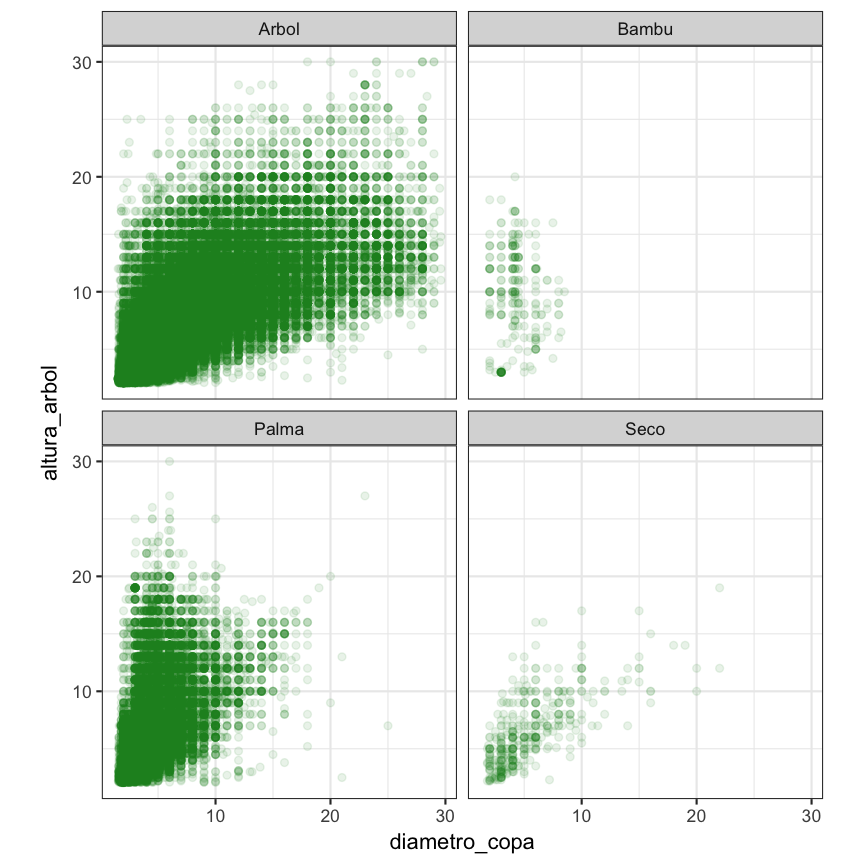
\includegraphics[width=1\linewidth]{tesis-unigis_files/figure-latex/au-veg-1} \caption{caraterísticas por tipo de vegetacion}\label{fig:au-veg}
\end{figure}

Otra característica interesante para buscar condiciones que afectan el
desarrollo del arbolado, representado por la altura y el diámetro son el
tipo de lugares que conforman el espacio público donde se encuentran el
mayor número de ellos. En la figura \ref{fig:au-emplaz-veg} se observa
la desagregación de los individuos por tipo de emplazamiento en gráficas
individuales de altura y diámetro, y en color el tipo de vegetación. Es
notorio en la figura que los parques urbanos y escenarios deportivos son
los equipamientos que mayor cantidad de individuos y más desarrollos
alojan. Caso aparte son los andenes y separadores viales como se ve en
la tabla \ref{tab:ca2015sel-emplazamiento} y el gráfico alojan 59.63\%
de los individuos. Esto puede ser un hecho que incita a incluir
elementos estructurales en los modelos que explican desde aspectos
estructurales de los barrios la cobertura de copa. Por supuesto las
rondas de ríos y canales dada su disponibilidad de agua condicionan el
desarrollo de los individuos arbóreos y su cantidad.

\begin{figure}
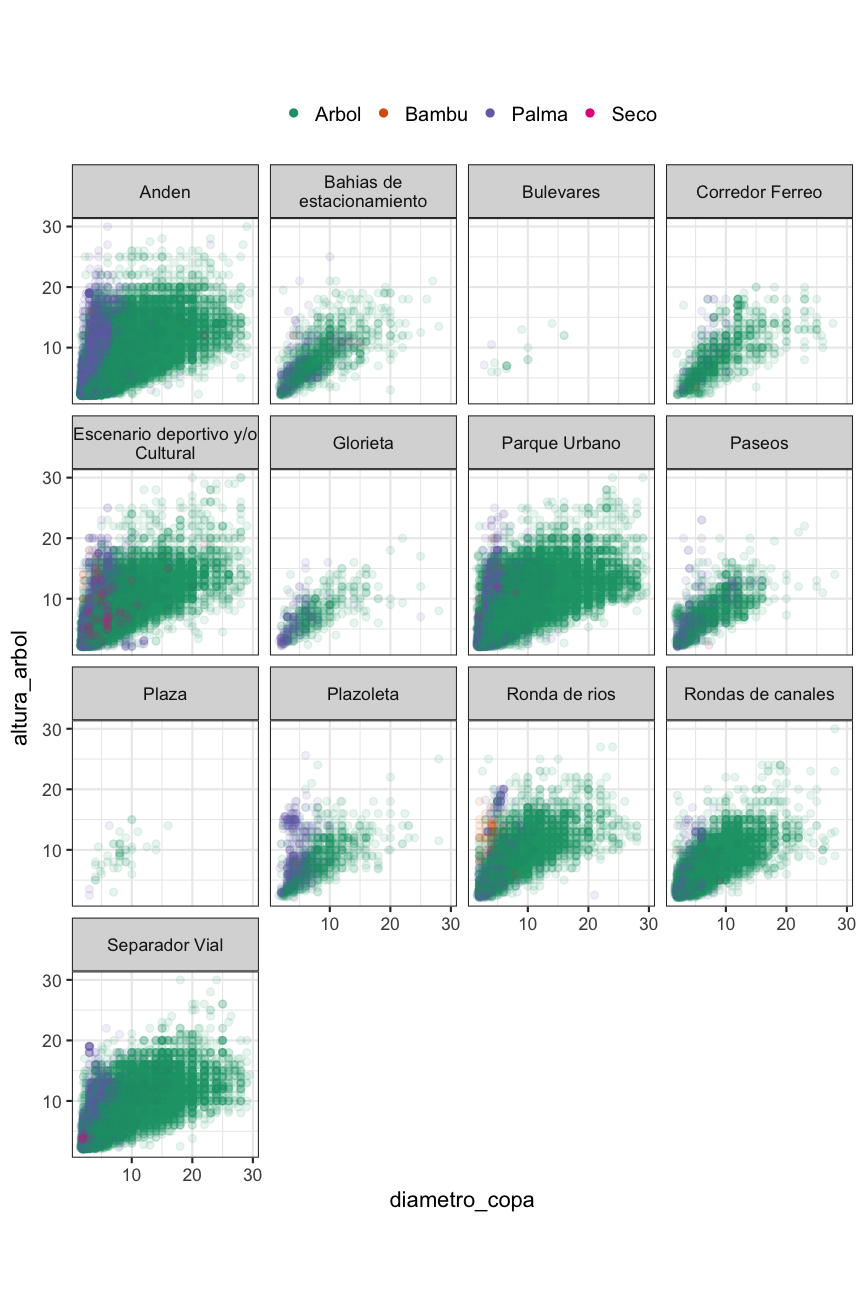
\includegraphics[width=1\linewidth]{tesis-unigis_files/figure-latex/au-emplaz-veg-1} \caption{Caraterísticas por tipo de vegetación y emplazamiento}\label{fig:au-emplaz-veg}
\end{figure}

Otra forma de ver los datos de resumen de las tabla
\ref{tab:ca2015sel-emplazamiento} y que completa la visión sobre la
distribución de los datos en relación al desarrollo físico de los
individuos arbóreos es la distribución de los diámetros (figura
\ref{fig:au-diametro-emp})y las alturas (figura \ref{fig:au-altura-emp})
en relación con el emplazamiento. En ambas gráficas el punto rojo
representa el valor promedio

\begin{figure}
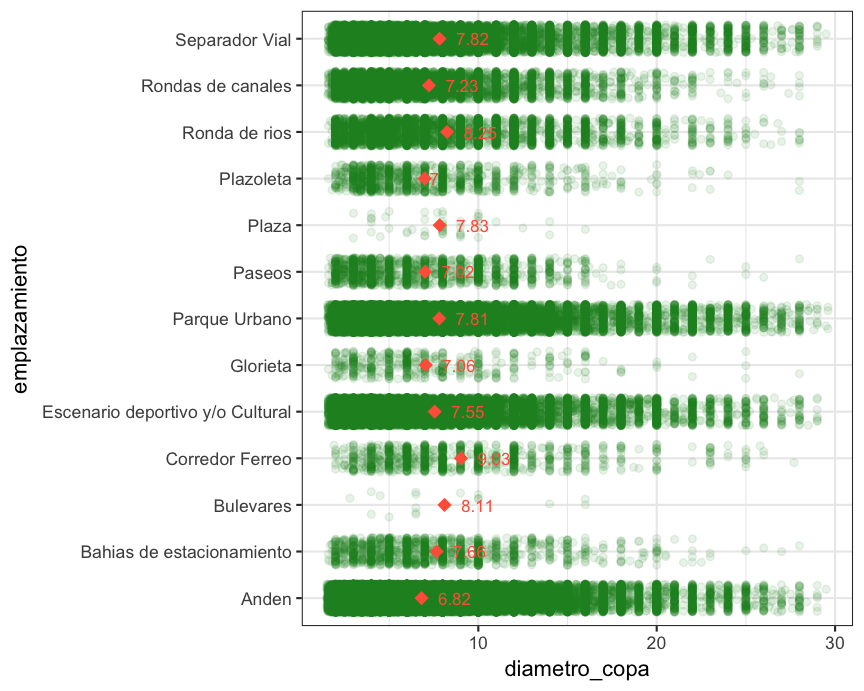
\includegraphics[width=1\linewidth]{tesis-unigis_files/figure-latex/au-diametro-emp-1} \caption{Variabilidad del diámetro de copa por emplazamiento}\label{fig:au-diametro-emp}
\end{figure}

\begin{figure}
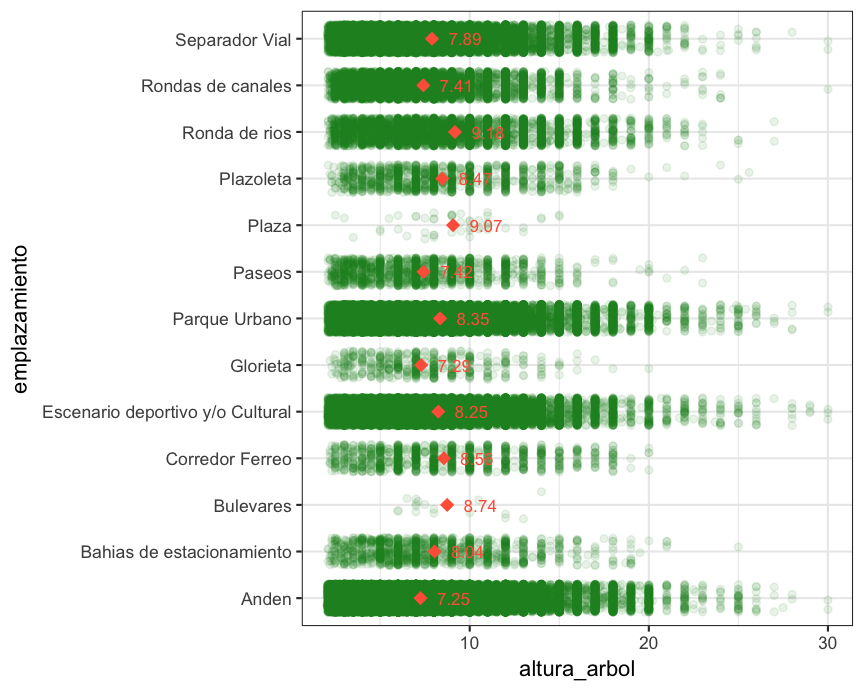
\includegraphics[width=1\linewidth]{tesis-unigis_files/figure-latex/au-altura-emp-1} \caption{Variabilidad de la altura de los arboles por emplazamiento}\label{fig:au-altura-emp}
\end{figure}

Finalmente en la figura \ref{fig:au-geo-emp} graficamos los individuos
en pequeños mapa por tipo de emplazamiento para observar su distribución
geográfica. Es notorio que los árboles están distribuidos en toda la
ciudad dada la disponibilidad de andenes aptos para alojarlos. Esto
invita a explorar la relación que pueda existir entre el tamaño de los
andenes de los barrios y el desarrollo físico de los individuos, ya que
las vías con separadores viales y en consecuencia con más espacio para
que árboles de mayor tamaño puedan desarrollarse es consistente con el
valor medio de la altura y el diámetro sean mayores que el de los
andenes. Sin embargo este hecho escapa del alcance de este trabajo y
puede ser indagado por otras investigaciones.

\begin{figure}
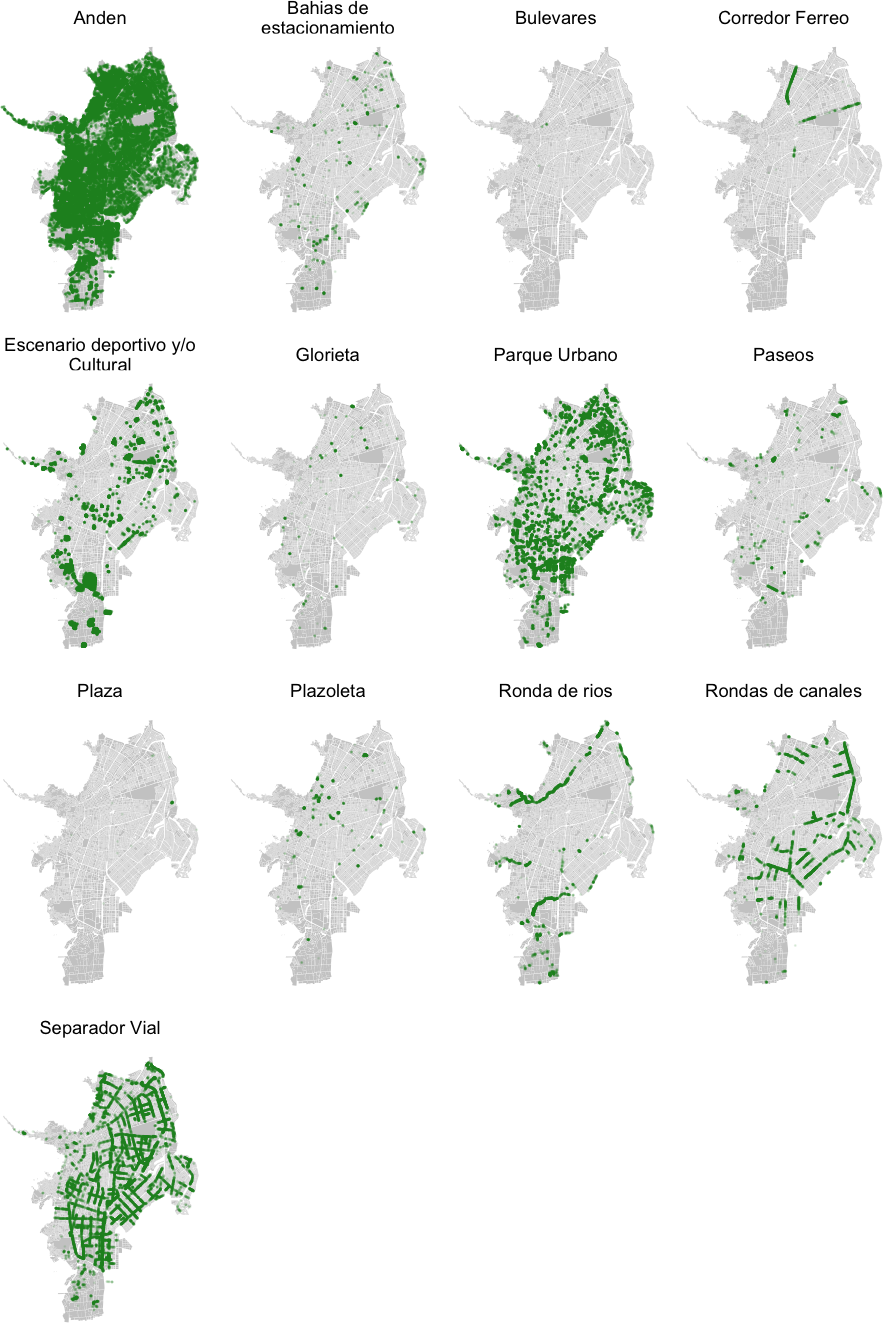
\includegraphics[width=1\linewidth]{tesis-unigis_files/figure-latex/au-geo-emp-1} \caption{Small multiples de los individuos arbóreos por emplazamiento}\label{fig:au-geo-emp}
\end{figure}

Antes de agregar (enmascarar) los datos usando los sectores censales es
interesante inspeccionar el efecto que tiene usar unidade regulares o de
tamaños no uniformes como los sectores urbanos en las coberturas de
copa. Para ello podemos usar hexágonos de 250 metros de ancho que cubren
completamente el territorio. La figura \ref{fig:au-geo-hex} se evidencia
que existen cinturones y lugares de alta concentración de individuos y
en consecuencia de mayor cobertura de copa.

\begin{figure}
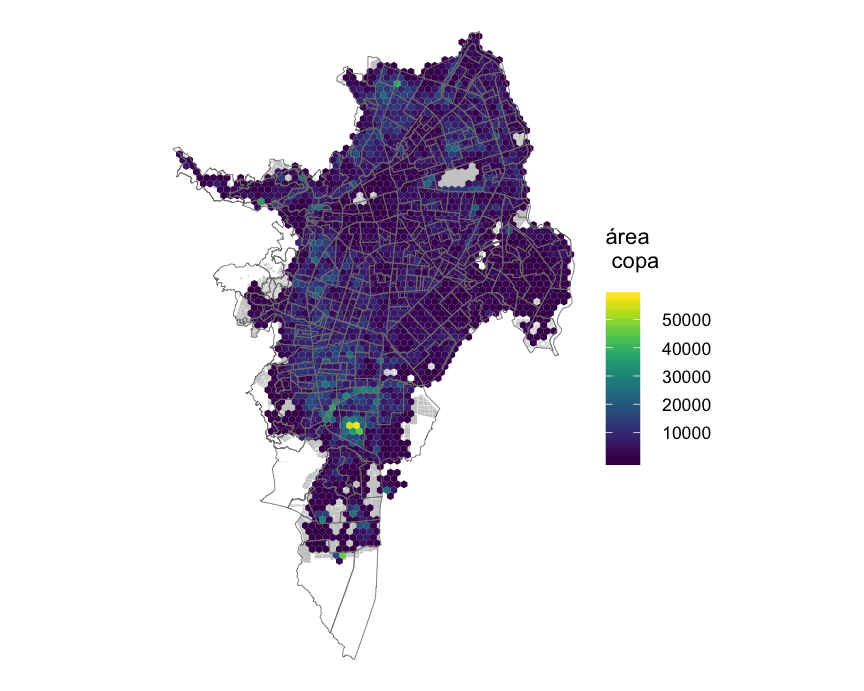
\includegraphics[width=1\linewidth]{tesis-unigis_files/figure-latex/au-geo-hex-1} \caption{Suma de cobertura por hexagonos}\label{fig:au-geo-hex}
\end{figure}

En la figura \ref{fig:au-su-acopa} usamos los SUs para agregar los
valores de área de copa. Se observa como se reduce un poco la
continuidad, y se intensifica el efecto de la agregación en algunos
sectores y se atenúa en otros (las figuras \ref{fig:comp-su-hex-copa} y
\ref{fig:comp-su-hex-numarb} muestran el efecto de la agregación en el
área de copa y en el número de individuos, respectivamente ).

\begin{figure}
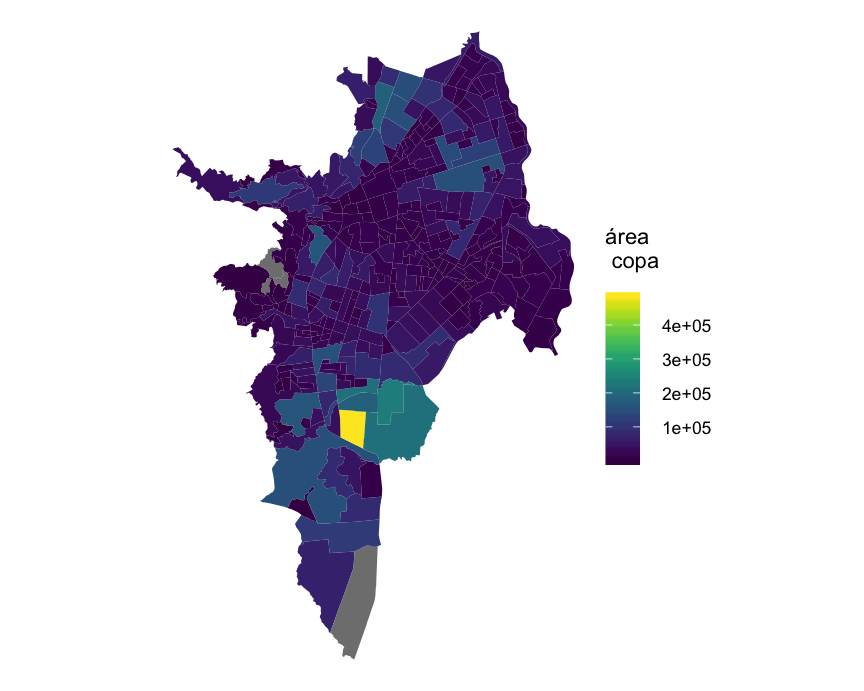
\includegraphics[width=1\linewidth]{tesis-unigis_files/figure-latex/au-su-acopa-1} \caption{Area de copa por sector censal}\label{fig:au-su-acopa}
\end{figure}

\begin{figure}
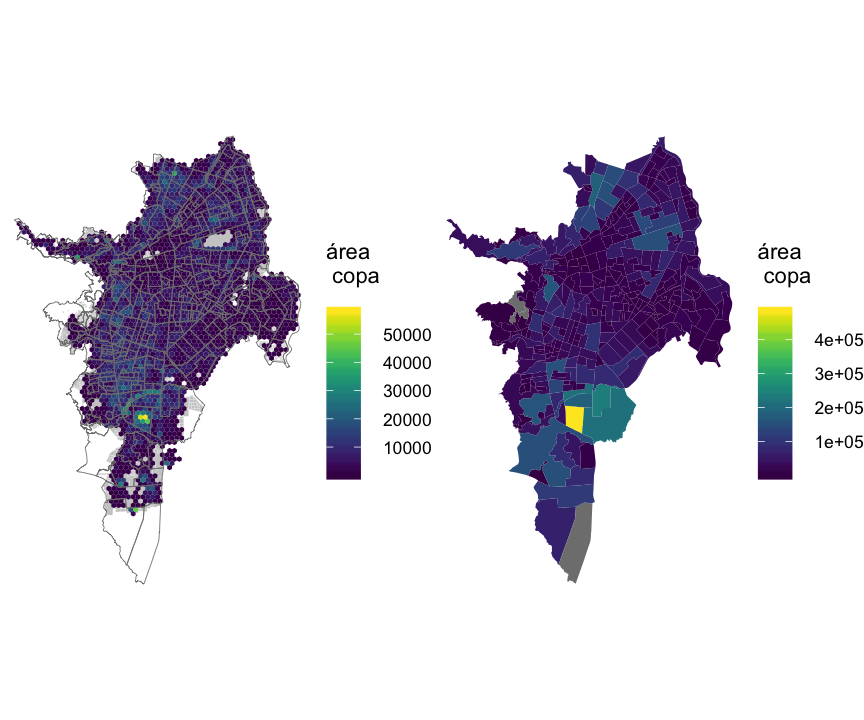
\includegraphics[width=1\linewidth]{tesis-unigis_files/figure-latex/comp-su-hex-copa-1} \caption{Agregación de area de copa por hexagonos y SU}\label{fig:comp-su-hex-copa}
\end{figure}

\begin{figure}
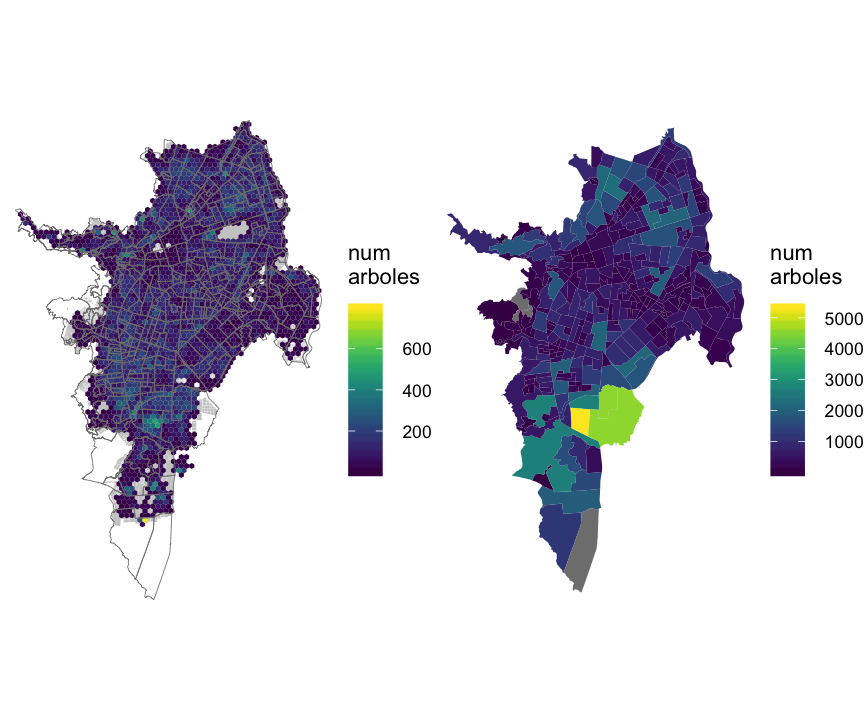
\includegraphics[width=1\linewidth]{tesis-unigis_files/figure-latex/comp-su-hex-numarb-1} \caption{Agregación de número de árboles por hexagonos y SU}\label{fig:comp-su-hex-numarb}
\end{figure}

Esto sugiere que usar valores porcentuales para la cobertura en relación
con el área de los SU o del área no-privada de cada sector puede ser una
mejor medida para caracterizar el beneficio real en cada sector censal.
En razón a esta consideración y las reflexiones sobre el tema en
\citet{schwarz_trees_2015}, que sugiere que la distinción entre áreas
privadas y públicas puede ayudar a determinar las superficies plantables
totales que están disponibles para aumentar la cobertura de copa.
Calculamos entonces el porcentaje de cobertura de copa respecto del área
total sector urbano y respecto del área de espacio público (área del
sector censal menos el área de las manzanas privadas)\footnote{La capa
  de espacio público consolidada previamente nos permite identificar las
  manzanas de un SU que son espacio público, y por tanto podemos obtener
  el área que es vía pública, las manzanas que son privadas y las
  manzanas que son espacio público. Así el área pública es igual a la
  suma del área de calle más las manzanas de espacio público o al área
  de SU menos el área de manzanas privadas}. Las medidas porcentuales
respecto del área total y pública permiten hacer una comparación más
justa entre las diferentes unidades pues relativiza los niveles totales
de área de copa. Un hecho que apoya el uso de medidas en relación al
espacio público de un sector censal es que el CA2015 solo se realizó
para la vegetación en lugares públicos, sobre la calle o vía pública.

En consecuencia se calcularon las métricas de área de copa en relación
al área del sector urbano (\texttt{cobertura\_copa.su}) y al área
pública del sector urbano (\texttt{cobertura\_copa.ap}). En la figura
\ref{fig:metricas-coberturacont} se ven los mapas en escala continua y
en la figura \ref{fig:metricas-coberturadeciles} se reproducen los
mismos mapas usando una escala en deciles. Visualmente, cobertura de
copa parece en espacio público parece aproximarse mejor a los patrones
de distribución que se evidencia cuando usamos la división uniforme del
terreno en hexágonos (figura \ref{fig:au-geo-hex}), razón por la cual la
preferiremos sobre \texttt{cobertura\_copa.su} para los análsis.

\begin{figure}
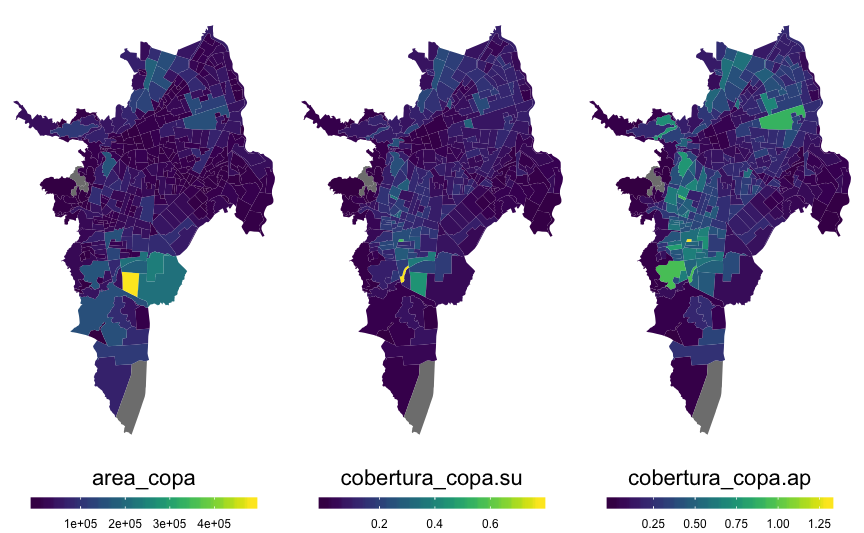
\includegraphics[width=1\linewidth]{tesis-unigis_files/figure-latex/metricas-coberturacont-1} \caption{Métricas de cobertura de copa: área neta, porcentaje respecto del sector censal y porcentaje respecto del área pública }\label{fig:metricas-coberturacont}
\end{figure}

\begin{figure}
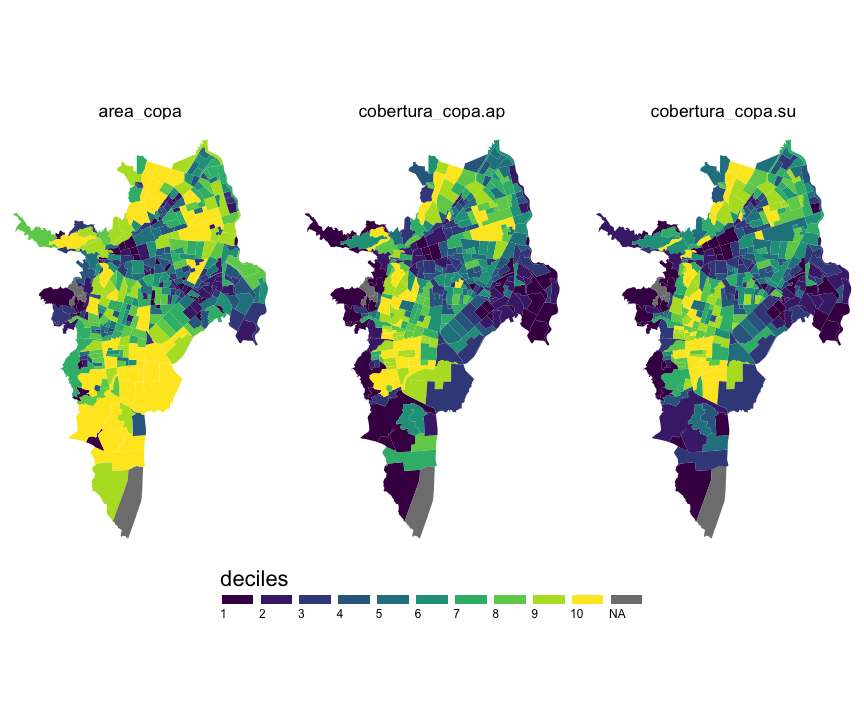
\includegraphics[width=1\linewidth]{tesis-unigis_files/figure-latex/metricas-coberturadeciles-1} \caption{Métricas de cobertura de copa: área neta, porcentaje respecto del sector censal y porcentaje respecto del área pública }\label{fig:metricas-coberturadeciles}
\end{figure}

Finalmente se muestra los histogramas y el resúmen de las métricas de
cobertura arbórea calculadas.

\begin{figure}
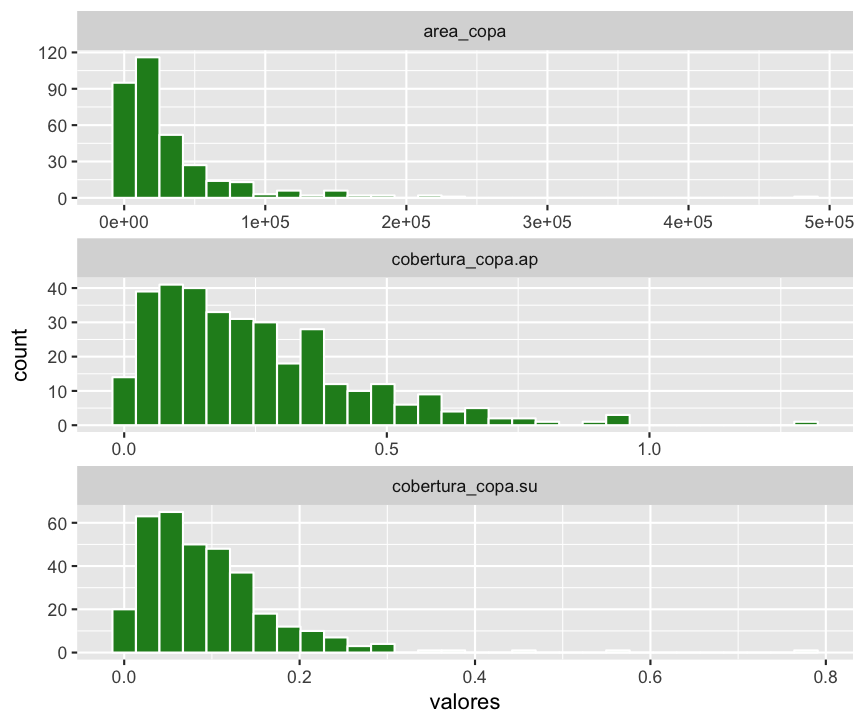
\includegraphics[width=1\linewidth]{tesis-unigis_files/figure-latex/hist-metricas-copa-1} \caption{Histograma de las métricas de la cobertura de copa}\label{fig:hist-metricas-copa}
\end{figure}

\begin{verbatim}
##    area_copa        cobertura_copa.su  cobertura_copa.ap 
##  Min.   :   429.2   Min.   :0.000769   Min.   :0.000877  
##  1st Qu.:  7708.5   1st Qu.:0.040890   1st Qu.:0.101541  
##  Median : 17651.6   Median :0.076651   Median :0.208246  
##  Mean   : 32949.9   Mean   :0.095847   Mean   :0.251747  
##  3rd Qu.: 39116.3   3rd Qu.:0.127404   3rd Qu.:0.349845  
##  Max.   :483719.9   Max.   :0.778169   Max.   :1.298912  
##  NA's   :4          NA's   :4          NA's   :4
\end{verbatim}

\section{Datos del censo de
población}\label{datos-del-censo-de-poblacion}

Los datos del censo fueron descargados del aplicativo con que cuenta el
DANE para dar acceso al censo de población 2005
\citep{censo_sistema_dane}. Los datos agregados por sectores censales
los inspeccionamos a través de los resúmenes estadistico, histogramas y
mapas, de forma análoga a lo realizado hasta ahora con el resto de
variables.

\subsection{Característica de la
población}\label{caracteristica-de-la-poblacion}

La tabla \ref{tab:vars-poblacion} resumen las variables consideradas
inicialmente en este trabajo, sin embargo, algunas de ellas no contienen
suficiente variabilidad o el número de individuos es muy bajo en
comparación con el total de la población. En la tabla
\ref{tab:totales-poblacion} se observa el bajo número de personas que
pertenecen al pueblo Rom (gitanos), Palenqueros de San Basilio
(departamento de Bolívar) y de Raizales del Archipiélago de San Andrés,
Providencia y Santa Catalina (SAI), por lo que son descartados del
análisis. La población indígena es también baja, pero no tanto como para
descartarla inmediatamente.

\begin{table}

\caption{\label{tab:totales-poblacion}Totales de población en la ciudad de Cali}
\centering
\begin{tabular}[t]{l|r}
\hline
Tipo & Cantidad\\
\hline
Población Total & 2027024\\
\hline
Población afrodescendiente, negros o mulatos & 530990\\
\hline
Población indígena & 9195\\
\hline
Población Rom & 690\\
\hline
Población Palenqueros & 1\\
\hline
Población raizales de SAI & 851\\
\hline
\end{tabular}
\end{table}

La figura \ref{fig:mapas-poblacion-cont} muestra los datos de las
variables de población en espacio geografico de la ciudad usando una
escala continua y la figura \ref{fig:mapas-poblacion-deciles} lo hace
usando una escala discreta (deciles).

\begin{figure}
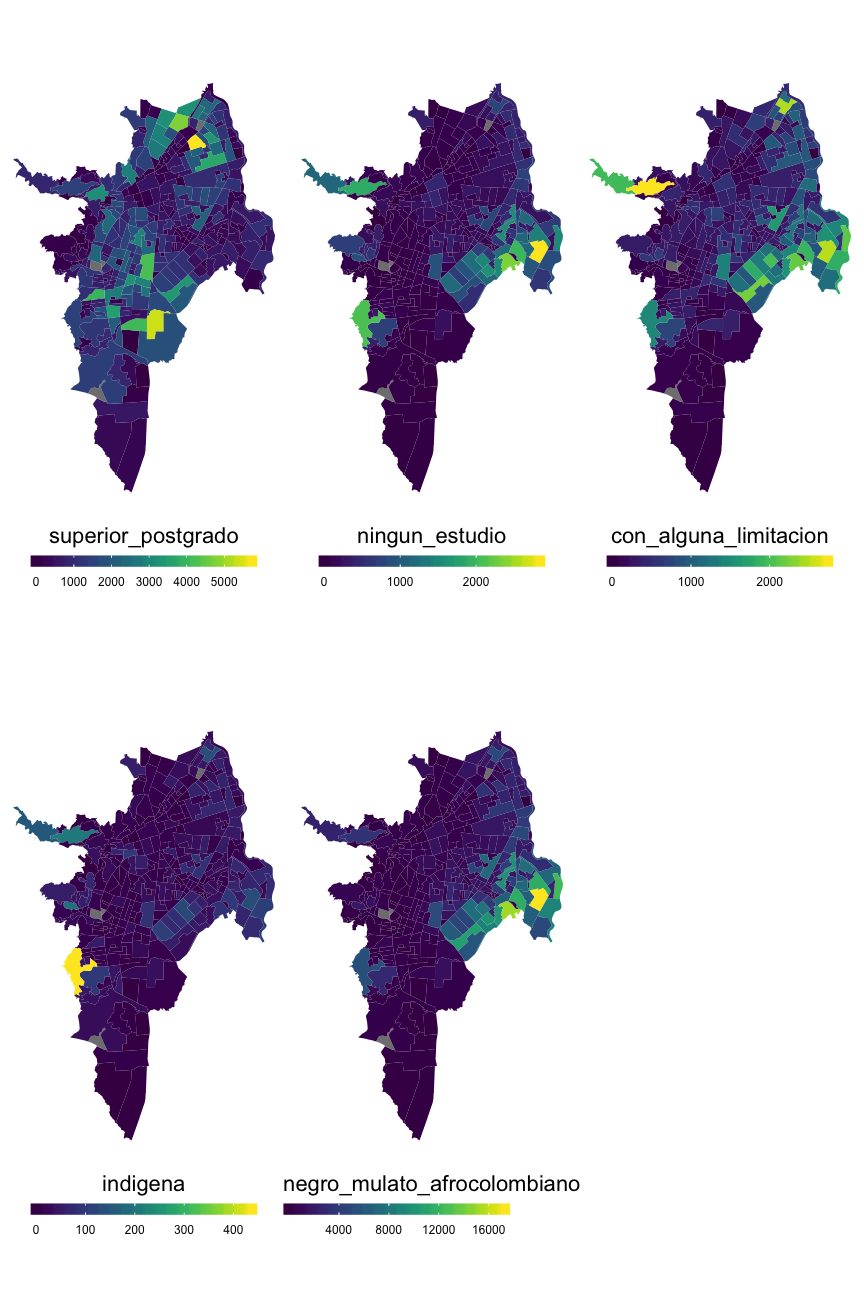
\includegraphics[width=1\linewidth]{tesis-unigis_files/figure-latex/mapas-poblacion-cont-1} \caption{Mapas de las variables de población seleccionadas (escala contínua)}\label{fig:mapas-poblacion-cont}
\end{figure}

\begin{figure}
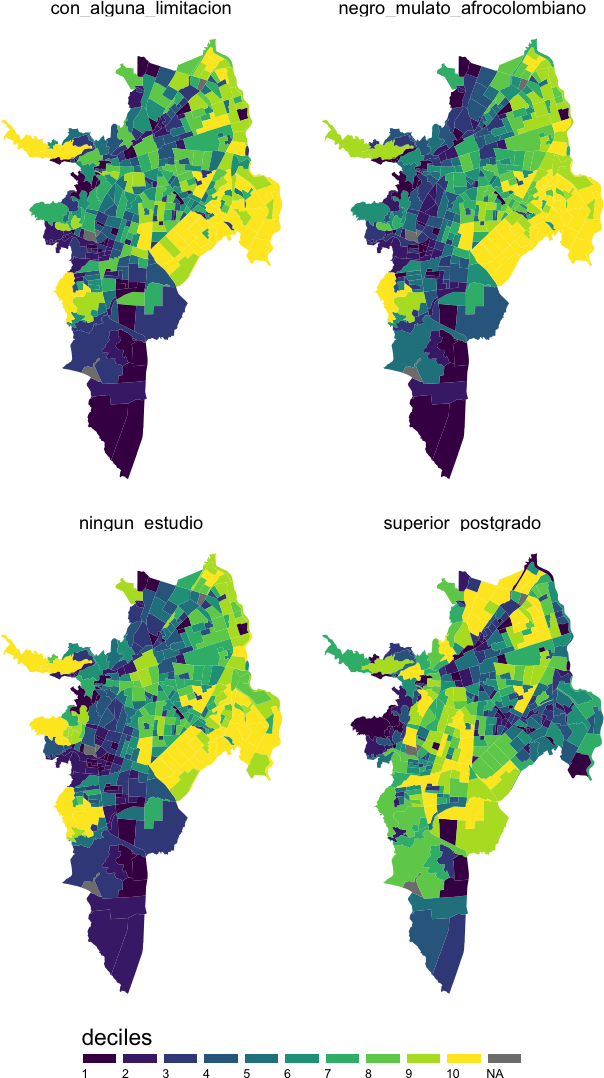
\includegraphics[width=1\linewidth]{tesis-unigis_files/figure-latex/mapas-poblacion-deciles-1} \caption{Mapas de las variables de población seleccionadas (en deciles)}\label{fig:mapas-poblacion-deciles}
\end{figure}

Los histogramas de estas variables en la figura \ref{fig:hist-poblacion}
siguen la tendencia que se ha venido observando en los histogramas de
cobertura arbórea y de variables de acceso a espacios verdes : las
distribuciones no son \emph{normales}, tienen una inclinación a la
derecha.

\begin{figure}
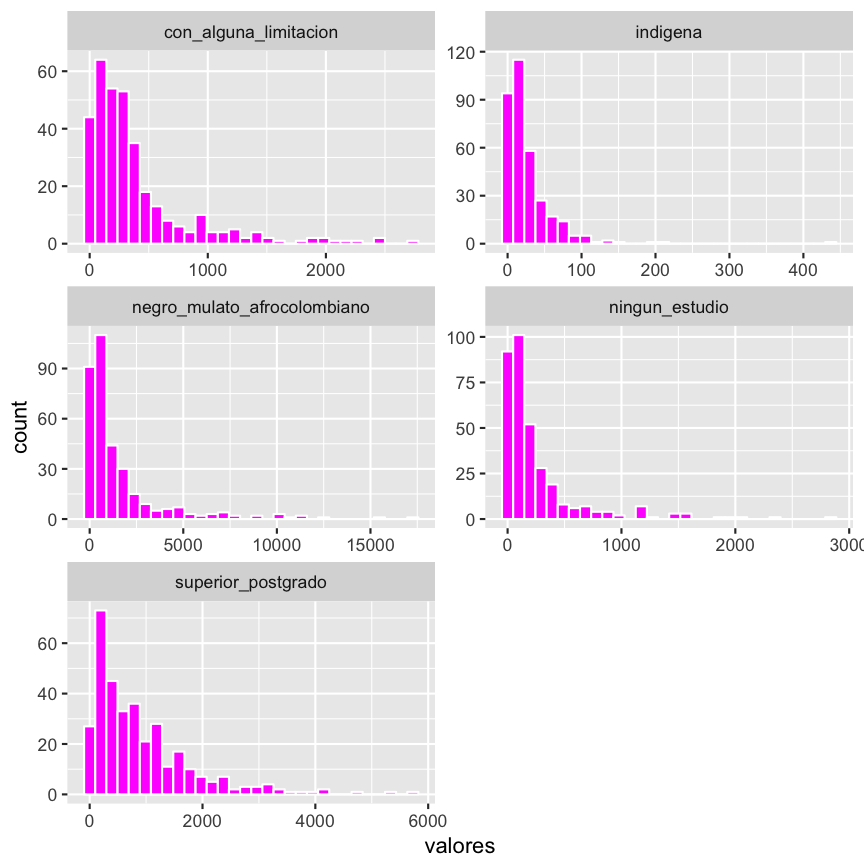
\includegraphics[width=1\linewidth]{tesis-unigis_files/figure-latex/hist-poblacion-1} \caption{Histogramas de las variables de población }\label{fig:hist-poblacion}
\end{figure}

Además de las variables seleccionadas podemos calcular indicadores que
se relacionan con el teóricamente como la densidad de población: dado
que los árboles compiten por el espacio con los seres humanos es de
esperarse que a mayor cantidad de personas haya menos lugar para los
árboles. Podemos de nuevo calcular indicadores porcentualización de las
condiciones de la población para facilitar la comparaciones y acentuar
las diferencias entre los diferente sectores.

A continuación se muestran los mapas en escala continua (figura
\ref{fig:mapas-poblacion-mod-cont}), discreta (figura
\ref{fig:mapas-poblacion-mod-deciles}) e histogramas (figura
\ref{fig:hist-poblacion-mod}) de los indicadores porcentuales de las
condiciones y la densidad de población.

\begin{figure}
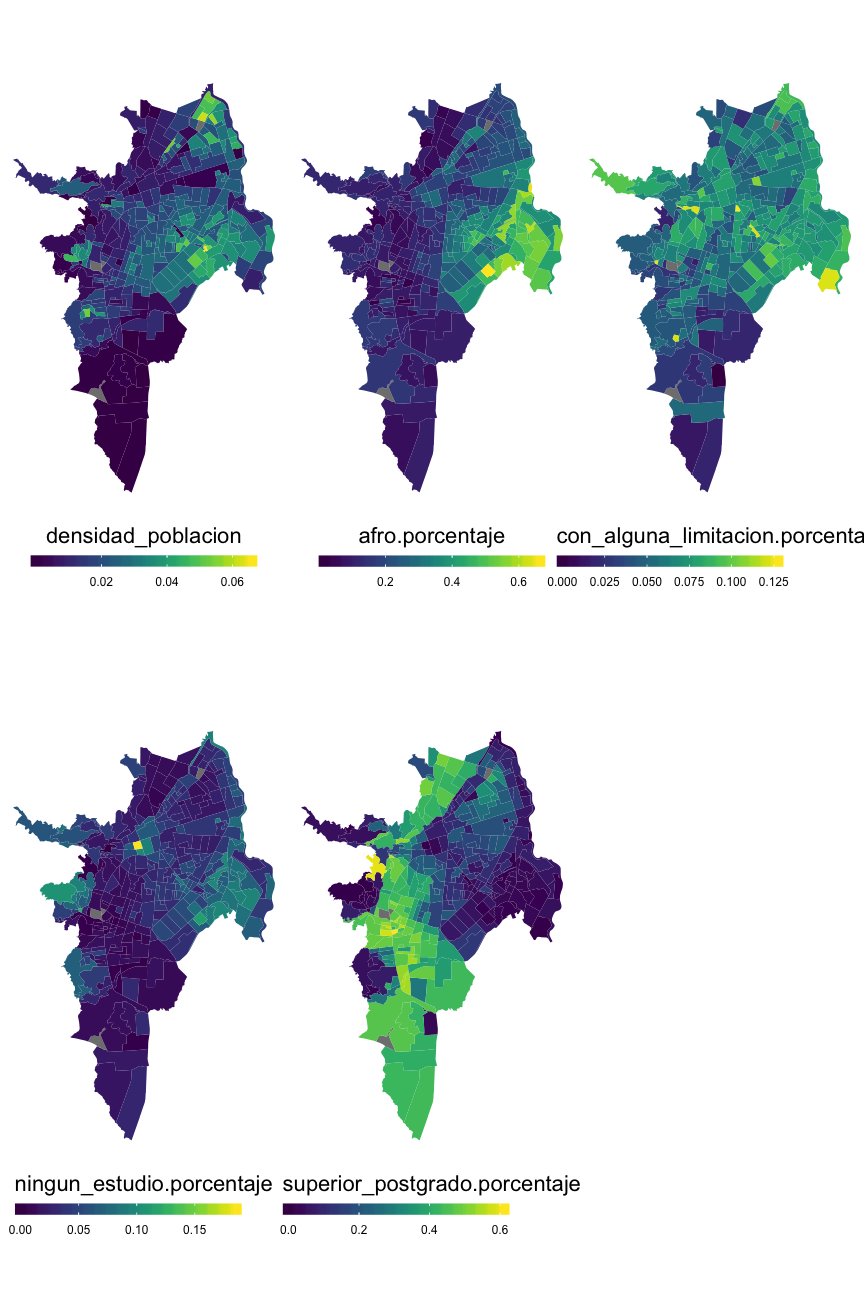
\includegraphics[width=1\linewidth]{tesis-unigis_files/figure-latex/mapas-poblacion-mod-cont-1} \caption{Mapas de las variables de población seleccionadas como porcentajes (escala contínua)}\label{fig:mapas-poblacion-mod-cont}
\end{figure}

\begin{figure}
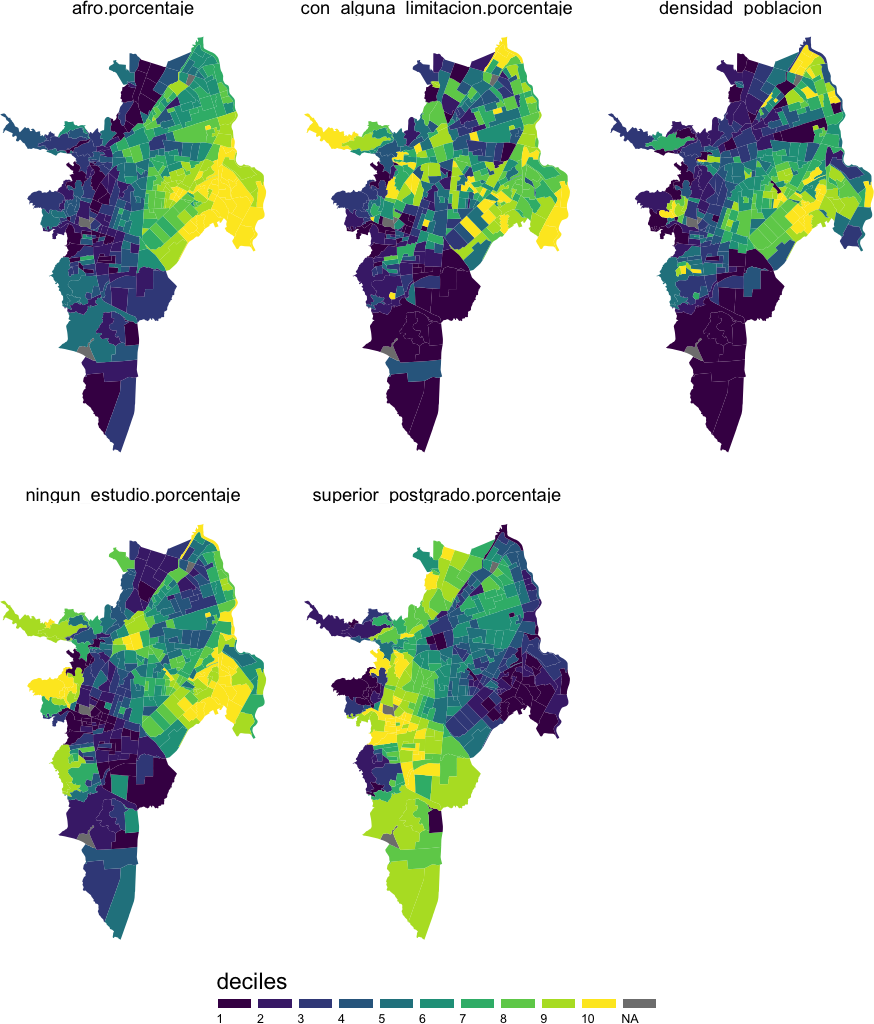
\includegraphics[width=1\linewidth]{tesis-unigis_files/figure-latex/mapas-poblacion-mod-deciles-1} \caption{Mapas de las variables de población seleccionadas como porcentajes (en deciles)}\label{fig:mapas-poblacion-mod-deciles}
\end{figure}

\begin{figure}
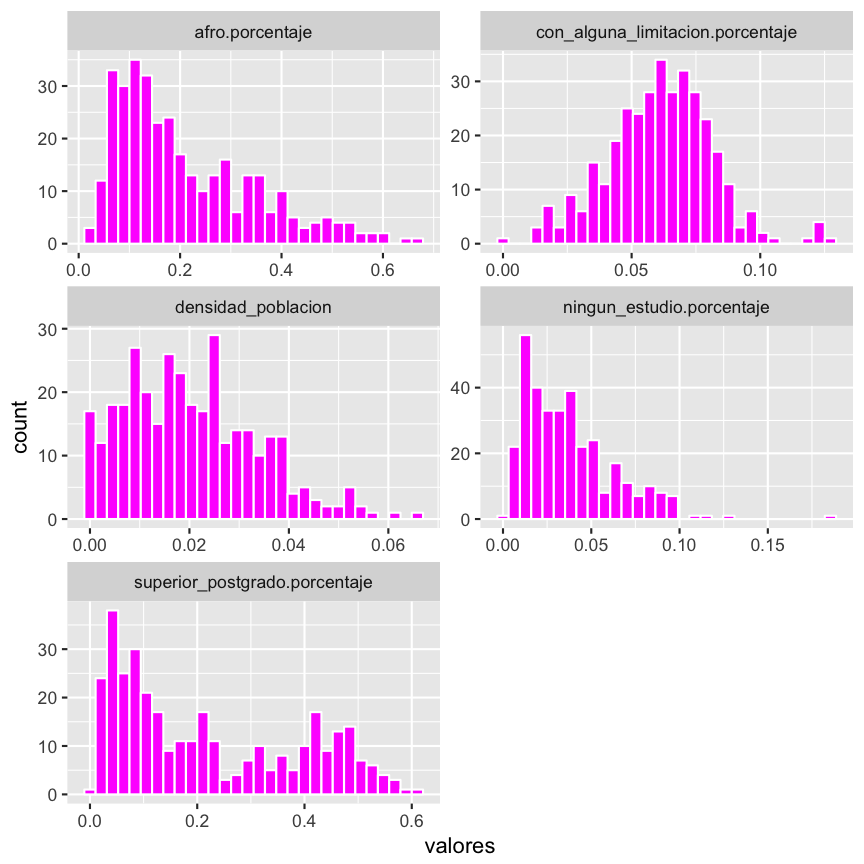
\includegraphics[width=1\linewidth]{tesis-unigis_files/figure-latex/hist-poblacion-mod-1} \caption{Histogramas de las variables de población como porcentaje}\label{fig:hist-poblacion-mod}
\end{figure}

Podemos notar que la transformación realizada al expresar las variables
como porcentaje reduce la inclinación hacia la derecha de los
histogramas e inclusive la corrige para el caso de personas con alguna
limitación.

Para finalizar con la inspección de los datos sobre la población se
proveen el resumen estadístico de las variables.

\begin{verbatim}
##  superior_postgrado ningun_estudio   con_alguna_limitacion
##  Min.   :   0.0     Min.   :   0.0   Min.   :   0.0       
##  1st Qu.: 234.8     1st Qu.:  43.0   1st Qu.: 102.0       
##  Median : 648.5     Median : 113.0   Median : 261.5       
##  Mean   : 907.2     Mean   : 254.3   Mean   : 394.5       
##  3rd Qu.:1229.8     3rd Qu.: 282.5   3rd Qu.: 454.8       
##  Max.   :5728.0     Max.   :2838.0   Max.   :2736.0       
##  NA's   :4          NA's   :4        NA's   :4            
##     indigena      negro_mulato_afrocolombiano densidad_poblacion
##  Min.   :  0.00   Min.   :    1.0             Min.   :0.000033  
##  1st Qu.:  6.00   1st Qu.:  273.5             1st Qu.:0.009483  
##  Median : 16.00   Median :  661.0             Median :0.018837  
##  Mean   : 26.89   Mean   : 1552.6             Mean   :0.020423  
##  3rd Qu.: 34.00   3rd Qu.: 1664.5             3rd Qu.:0.028885  
##  Max.   :437.00   Max.   :17264.0             Max.   :0.065882  
##  NA's   :4        NA's   :4                   NA's   :4         
##  afro.porcentaje   con_alguna_limitacion.porcentaje
##  Min.   :0.01683   Min.   :0.00000                 
##  1st Qu.:0.10407   1st Qu.:0.04866                 
##  Median :0.17150   Median :0.06197                 
##  Mean   :0.21087   Mean   :0.06109                 
##  3rd Qu.:0.28770   3rd Qu.:0.07422                 
##  Max.   :0.66255   Max.   :0.12729                 
##  NA's   :4         NA's   :4                       
##  ningun_estudio.porcentaje superior_postgrado.porcentaje
##  Min.   :0.00000           Min.   :0.00000              
##  1st Qu.:0.01690           1st Qu.:0.06914              
##  Median :0.03161           Median :0.16845              
##  Mean   :0.03766           Mean   :0.22020              
##  3rd Qu.:0.05050           3rd Qu.:0.38509              
##  Max.   :0.18548           Max.   :0.61056              
##  NA's   :4                 NA's   :4
\end{verbatim}

\subsection{Características de las
viviendas}\label{caracteristicas-de-las-viviendas}

Además de las rasgos étnicos, condiciones de estudio y limitaciones de
la población el censo de 2005 tiene disponibles datos sobre el tipo de
viviendas (casa, apartamento, tipo cuarto, casa indígena, otros), y el
uso habitacional, comercial y la cantidad de unidades especiales de
alojamiento L.E.A dado a los predios. La vocación comercial o
residencial de un barrio puede ser un factor en el desarrollo del
arbolado urbano, ya sea por las condiciones físicas como por la
intervención de sus habitantes. Estas variables pueden también
expresarse como porcentaje de la cantidad de predios de vivienda en el
caso de los tipos o como porcentaje de la cantidad de predios en el caso
del uso como unidad de vivienda, económica o L.E.A.

A continuación presentamos el resumen, los mapas por sector urbano
(figuras \ref{fig:mapas-usopredios-cont} y
\ref{fig:mapas-usopredios-deciles})y los histogramas (figura
\ref{fig:hist-usopredios})de las variables sobre el uso de los predios.

\begin{figure}
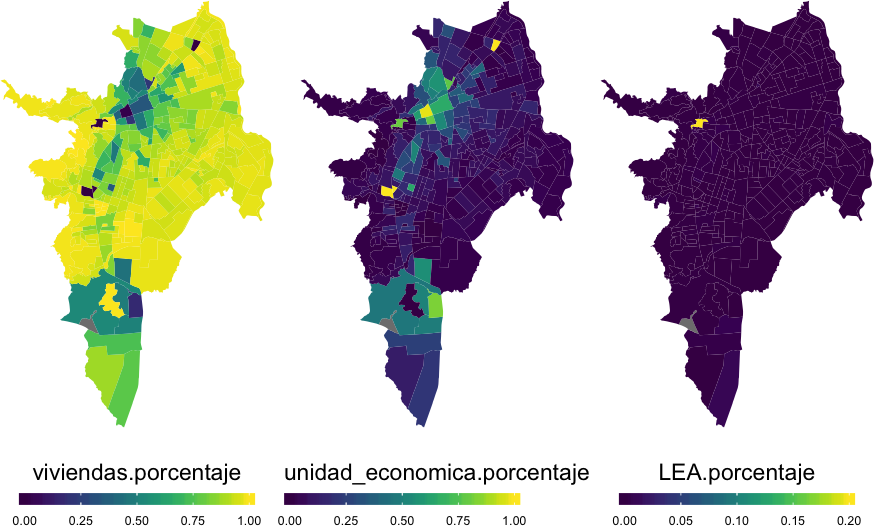
\includegraphics[width=1\linewidth]{tesis-unigis_files/figure-latex/mapas-usopredios-cont-1} \caption{Mapas de las variables sobre el tipo de uso de los predios como porcentaje de la cantidad de predios (escala contínua)}\label{fig:mapas-usopredios-cont}
\end{figure}

\begin{figure}
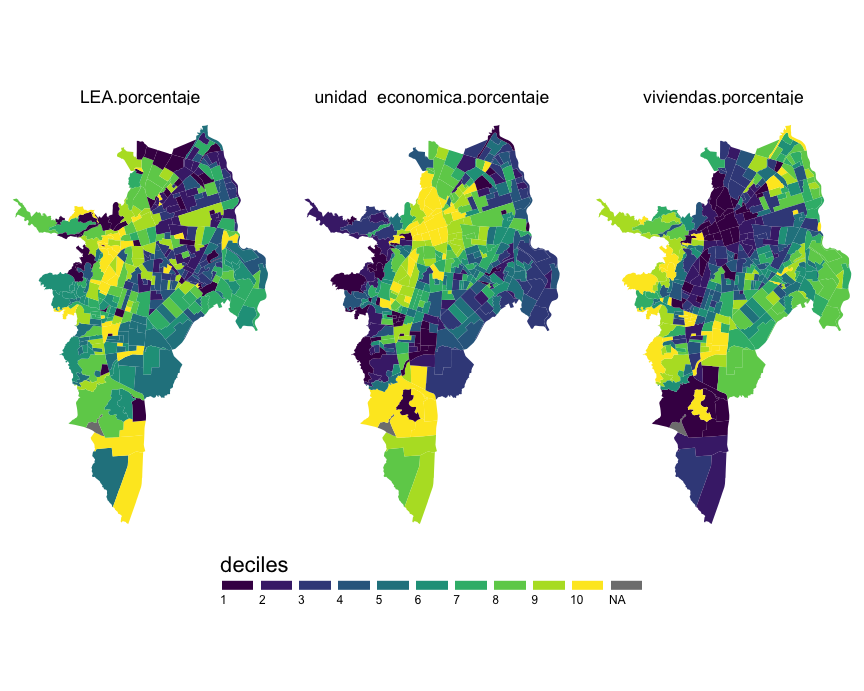
\includegraphics[width=1\linewidth]{tesis-unigis_files/figure-latex/mapas-usopredios-deciles-1} \caption{Mapas de las variables sobre el tipo de uso de los predios como porcentaje de la cantidad de predios (en deciles)}\label{fig:mapas-usopredios-deciles}
\end{figure}

\begin{figure}
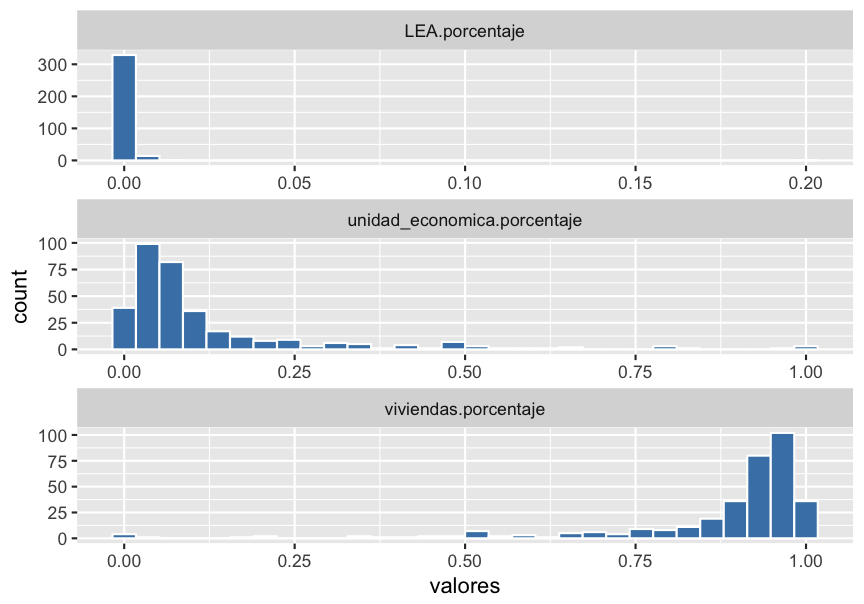
\includegraphics[width=1\linewidth]{tesis-unigis_files/figure-latex/hist-usopredios-1} \caption{Histogramas de las variables de uso de predios como porcentaje}\label{fig:hist-usopredios}
\end{figure}

El uso de L.E.A tiene una distribución concentrada en uno pocos SU, por
lo que podemos descartarla para los análisis de regresión. Existe
también cierta complementariedad entre el uso de vivienda y los usos
económicos de los predios, porque seguramente, si existe una correlación
entre estas variables y la cobertura de copa o el acceso a espacios
verdes una de las dos puede bastar para incluir esta dimensión en los
modelos de regresion.

A continuación presentamos el resumen, los mapas por sector urbano
(figuras \ref{fig:mapas-viviendas-cont} y
\ref{fig:mapas-viviendas-deciles})y los histogramas (figura
\ref{fig:hist-viviendas})de las variables sobre los tipos de vivienda.

\begin{figure}
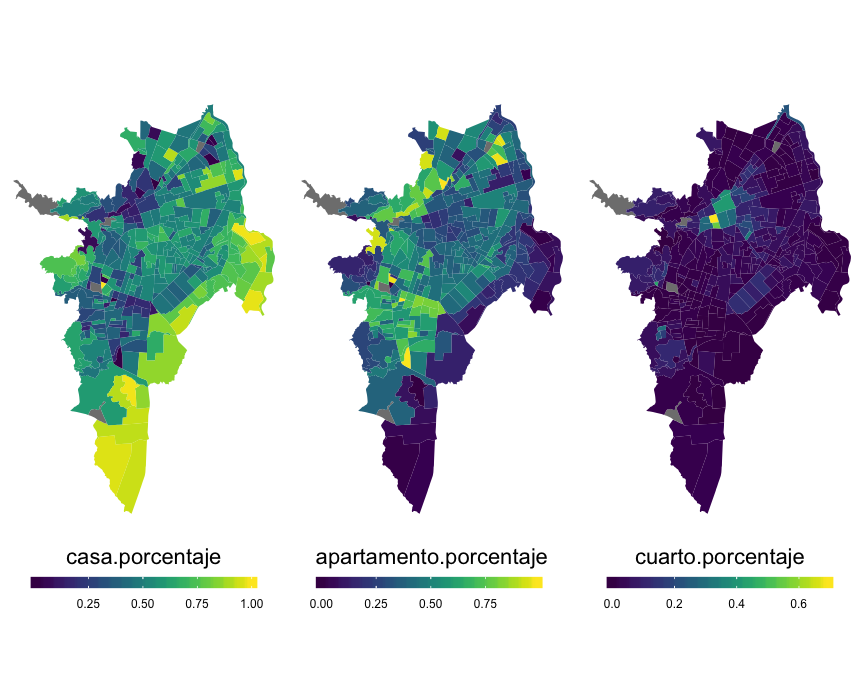
\includegraphics[width=1\linewidth]{tesis-unigis_files/figure-latex/mapas-viviendas-cont-1} \caption{Mapas de las variables sobre el tipo viviendas como porcentaje (escala contínua)}\label{fig:mapas-viviendas-cont}
\end{figure}

\begin{figure}
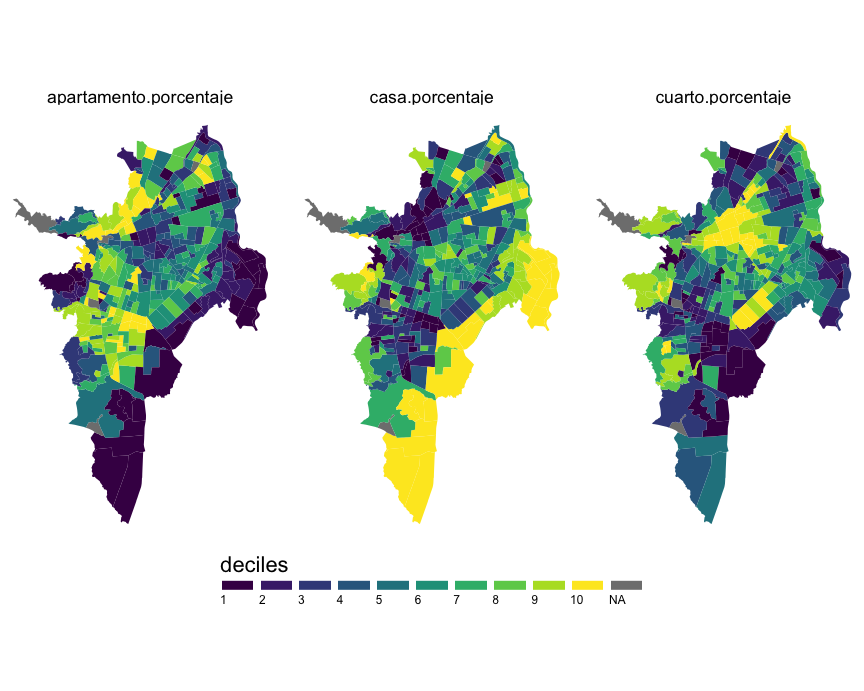
\includegraphics[width=1\linewidth]{tesis-unigis_files/figure-latex/mapas-viviendas-deciles-1} \caption{Mapas de las variables sobre el tipo viviendas como porcentaje (en deciles)}\label{fig:mapas-viviendas-deciles}
\end{figure}

\begin{figure}
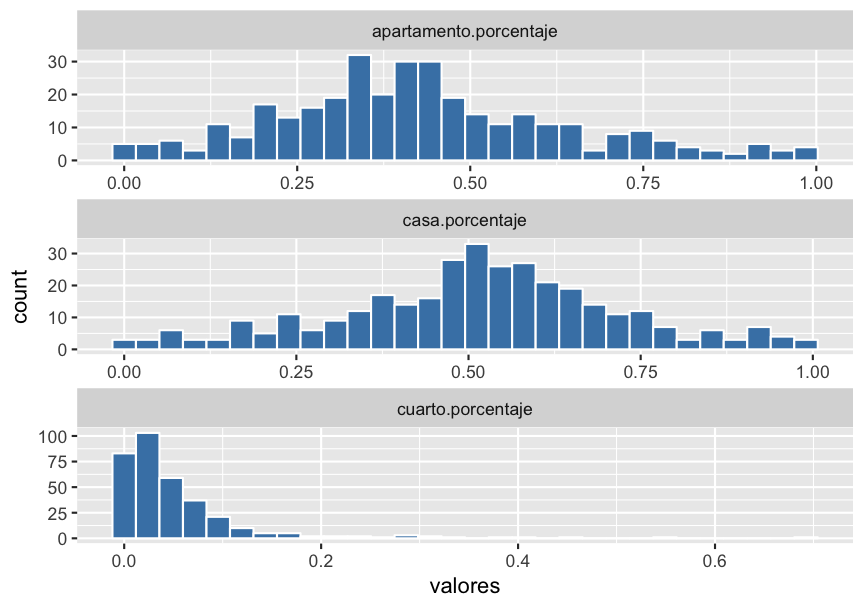
\includegraphics[width=1\linewidth]{tesis-unigis_files/figure-latex/hist-viviendas-1} \caption{Histogramas de los tipo de vivienda como porcentaje}\label{fig:hist-viviendas}
\end{figure}

Esta primera inspección a los datos permitió descartar algunas variables
a usar en los modelos de regresión sobre las coberturas y los espacios
verdes, conocer la distribución espacial de los datos y perfilar las
posibles variables a incluir. Sin embargo, la percepción suele ser
engañosa, vemos patrones en todas partes, así que es necesario acompañar
estas intuiciones con métricas estadísticas y gráficas sobre las
relaciones entre las variables dependientes e independientes para ser
más asertivos en las decisiones del proceso de modelado.

\section{Análisis estadísticos}\label{analisis-estadisticos}

\subsection{Criterios y selección de sectores
censales}\label{criterios-y-seleccion-de-sectores-censales}

Antes de iniciar un analaisis de regresion es importante establecer
ciertos criterios pra inclusion o no de ciertos datos dentro del
conjunto de varores para la regresion y calculo de la correlacion. Estos
criterios estan ligados creterios de excepcion de sectores urbanos a ser
incluidos en el analsis de regresion:

\begin{itemize}
\tightlist
\item
  sectores sin personas
\item
  sectores sin viviendas
\item
  sectores area de espacio publico mayor que el 60 \% del area del
  sector
\item
  sectores area de calle mayor que el 80 \% del area del sector
\item
  sectores area privada mayor que el 90 \% del area del sector
\end{itemize}

\begin{Shaded}
\begin{Highlighting}[]
\NormalTok{ analisis.cali.df }\OperatorTok\StringTok{ }
\StringTok{   }\KeywordTok{filter}\NormalTok{(}\KeywordTok{is.na}\NormalTok{(personas_edad)) }\OperatorTok
\StringTok{   }\KeywordTok{select}\NormalTok{(SETU_CCDGO) ->}\StringTok{ }\NormalTok{sin_personas}
 
\NormalTok{ analisis.cali.df }\OperatorTok\StringTok{ }
\StringTok{   }\KeywordTok{filter}\NormalTok{(uso_vivienda }\OperatorTok{==}\StringTok{ }\DecValTok{0}\NormalTok{) }\OperatorTok
\StringTok{   }\KeywordTok{select}\NormalTok{(SETU_CCDGO) ->}\StringTok{ }\NormalTok{sin_viviendas}

\NormalTok{ analisis.cali.df }\OperatorTok\StringTok{ }
\StringTok{   }\KeywordTok{filter}\NormalTok{(area_ep.porcentaje }\OperatorTok{>}\StringTok{ }\FloatTok{0.6}\NormalTok{ ) }\OperatorTok
\StringTok{   }\KeywordTok{select}\NormalTok{(SETU_CCDGO)  ->}\StringTok{ }\NormalTok{ep_}\DecValTok{60}
 
\NormalTok{ analisis.cali.df }\OperatorTok\StringTok{ }
\StringTok{   }\KeywordTok{filter}\NormalTok{(area_privada.porcentaje }\OperatorTok{>}\StringTok{ }\FloatTok{0.85}\NormalTok{ ) }\OperatorTok
\StringTok{   }\KeywordTok{select}\NormalTok{(SETU_CCDGO) ->}\StringTok{ }\NormalTok{privada_}\DecValTok{85}
 
\NormalTok{ analisis.cali.df }\OperatorTok\StringTok{ }
\StringTok{   }\KeywordTok{filter}\NormalTok{(area_calle.porcentaje }\OperatorTok{>}\StringTok{ }\FloatTok{0.8}\NormalTok{ ) }\OperatorTok
\StringTok{   }\KeywordTok{select}\NormalTok{(SETU_CCDGO) ->}\StringTok{ }\NormalTok{calle_}\DecValTok{80}
 
\NormalTok{ analisis.cali.df }\OperatorTok\StringTok{ }
\StringTok{   }\KeywordTok{filter}\NormalTok{(}\KeywordTok{is.na}\NormalTok{(area_copa)) }\OperatorTok
\StringTok{   }\KeywordTok{select}\NormalTok{(SETU_CCDGO) ->}\StringTok{ }\NormalTok{sin_arboles_censado}
 
 
\NormalTok{ su.exc.apriori<-}\KeywordTok{c}\NormalTok{(}\StringTok{"0204"}\NormalTok{,}\StringTok{"1736"}\NormalTok{,}\CommentTok{# sector con alto porcentaje no urbanizado}
                   \StringTok{"1709"}\NormalTok{,}\CommentTok{# maroria del area por fuera del perimetro urbano}
                   \StringTok{"1317"}\NormalTok{)}\CommentTok{# laguna del pandaje}
\end{Highlighting}
\end{Shaded}

Además de estos criterios se excluyeron los sectores donde está la
Laguna el Pondaje, que cubre una porción muy importante del sector que
no se ve reflejado en las otras métricas, los sectores con una porción
mayor al 60\% por fuera del perímetro urbano o sin urbanización visible
en las imagenes satelitales. Así los sectores excluidos del análisis se
muestran en los mapas \ref{fig:mapa-excluidos} y
\ref{fig:mapa-excluidos-tipo} por criterio usado.

\begin{figure}
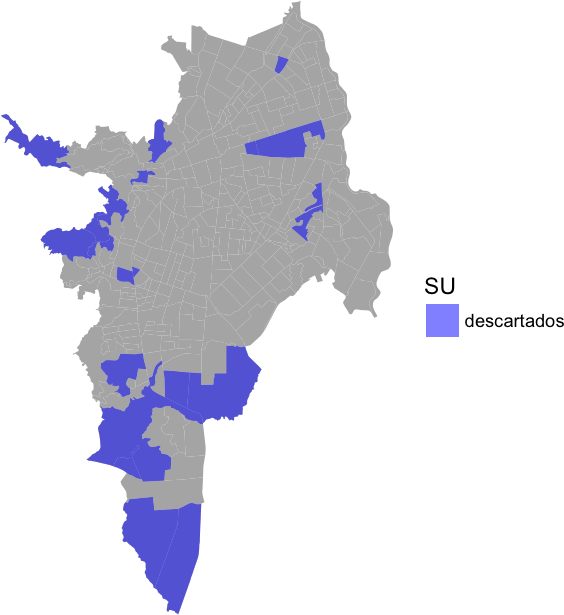
\includegraphics[width=1\linewidth]{tesis-unigis_files/figure-latex/mapa-excluidos-1} \caption{Mapa de los sectores excluidos}\label{fig:mapa-excluidos}
\end{figure}

\begin{figure}
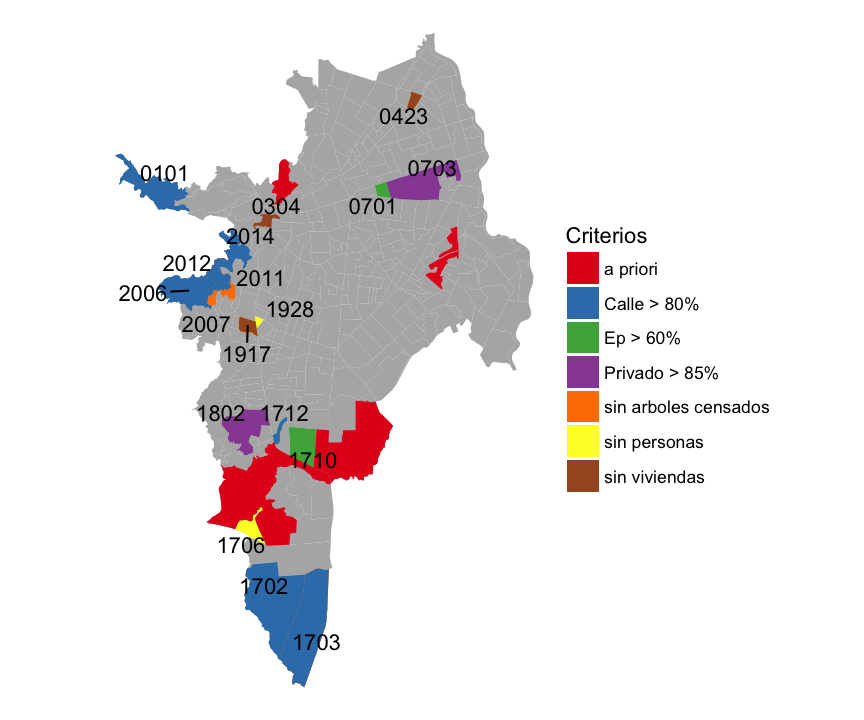
\includegraphics[width=1\linewidth]{tesis-unigis_files/figure-latex/mapa-excluidos-tipo-1} \caption{Mapa de los sectores excluidos por criterio usado}\label{fig:mapa-excluidos-tipo}
\end{figure}

Para el análisis de las zonas verdes, no se tiene en cuenta el criterio
de exclusión de SU sin árboles y se incluye la Laguna del Pondaje. Los
mapas de las zonas se ven el la figura \ref{fig:mapa-excluidos-ev} y
\ref{fig:mapa-excluidos-tipo-ev}.

\begin{figure}
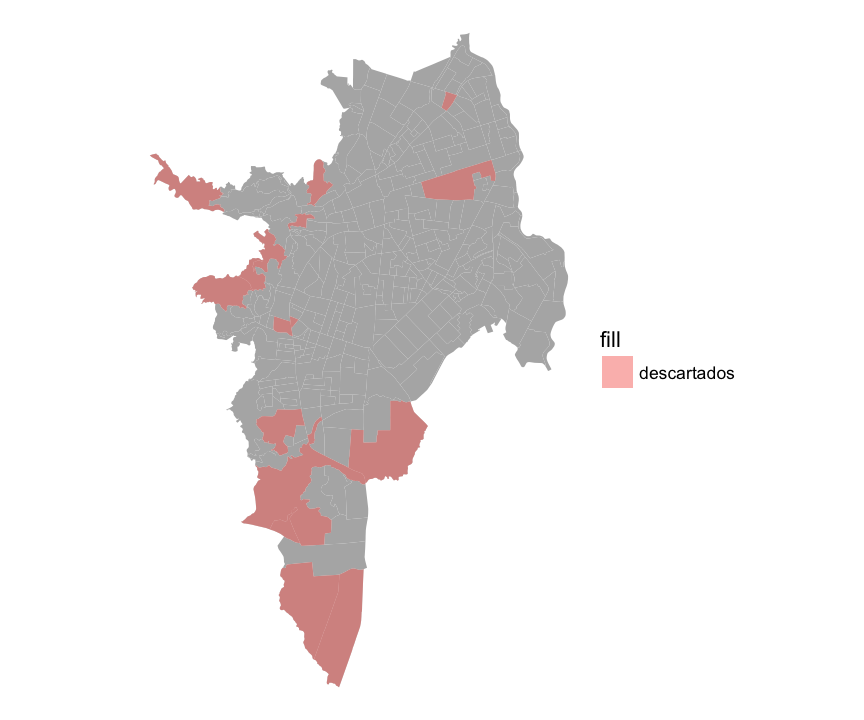
\includegraphics[width=1\linewidth]{tesis-unigis_files/figure-latex/mapa-excluidos-ev-1} \caption{Mapa de los sectores excluidos para el análisis de EV}\label{fig:mapa-excluidos-ev}
\end{figure}

\begin{figure}
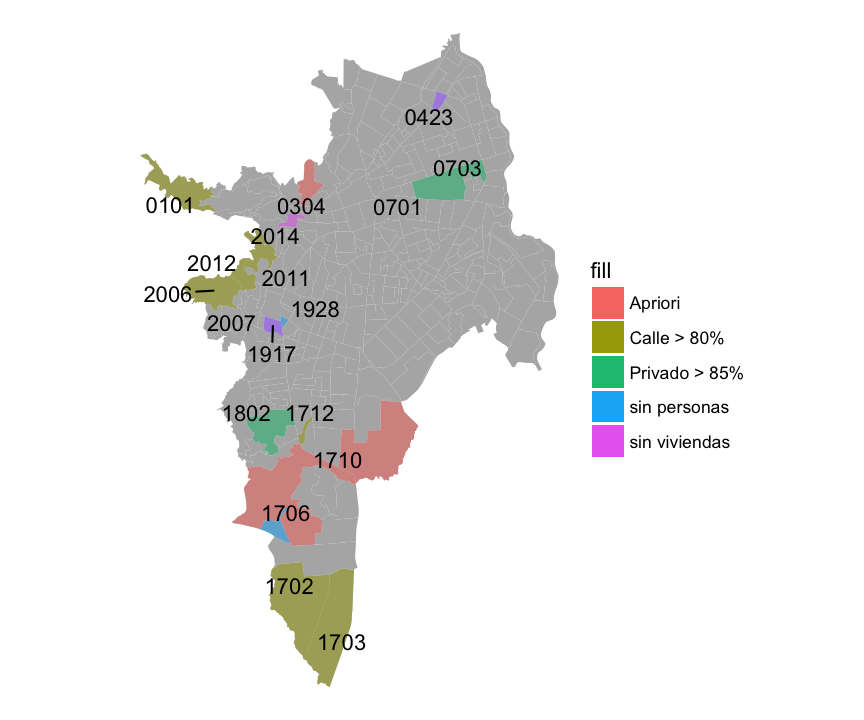
\includegraphics[width=1\linewidth]{tesis-unigis_files/figure-latex/mapa-excluidos-tipo-ev-1} \caption{Mapa de los sectores excluidos por criterio usado para el análisis de EV}\label{fig:mapa-excluidos-tipo-ev}
\end{figure}

\subsection{Modelando la cobertura de
copa}\label{modelando-la-cobertura-de-copa}

Las variables a incluir en los modelos lineales deben cumplir una serie
de condiciones para ser elegidas como candidatas:

\begin{itemize}
\tightlist
\item
  \emph{Mostrar una correlación fuerte} (típicamente mayor a 0.6 se
  considera una asociación fuerte).
\item
  \emph{Las variables independientes o predictoras no deben estar
  fuertemente correlacionadas entre ellas}.
\item
  \emph{Las observaciones deben ser independientes}. En nuestro caso
  significa que no debe existir relación espacial o temporal entre los
  diferentes sectores. Justamente esto se pondrá a prueba con los test
  estadísticos y los graficos de diagnostico sobre la distribución de
  los residuos de la regresión: se espera que dicha dependencia esté
  motivada por la vecindad de los sectores.
\item
  \emph{Las variables dependientes e independientes deben tener una
  distribución normal}. Esta condición no suele ser estricta, pues lo
  importante es que al calcular los coeficientes de la regresión
  obtengamos una distribución normal de los residuos (sin ningún patrón,
  ruido). De no ser así, es posible que las variables no sean
  independientes o que exista información significativa en los residuos,
  por ejemplo, porque existe autocorrelación espacial en la variable
  dependiente y entonces la regresión lineal no obtiene resultados
  confiables para los coeficientes.
\end{itemize}

Para hacer más tratable y gradual el proceso de complejizar el modelo
iniciaremos el análisis con las variables sobre la población, que son
las de mayor interés en un estudio dado su enfoque en la justicia
ambiental, para luego incorporar las variables de los dominios
relacionados con el uso de los predios, los tipos de viviendas y la
existencia de espacios verdes como parques, bulevares, escenarios
deportivos o plazas, que como se vio en la sección \ref{sec-ca2015}
(revisar figura \ref{fig:au-emplaz-veg}) alojan una cantidad
considerable de los individuos arbóreos de la ciudad.

Las variables a modelar son la área de copa en metros\textsuperscript{2}
(\texttt{area\_copa}) y la cobertura de copa como porcentaje del área
pública total (\texttt{cobertura\_copa.ap}), conformda por la vías y
calles más el área de espacio públicos) (ver figura
\ref{fig:mapa-copa-dep}).

\begin{figure}
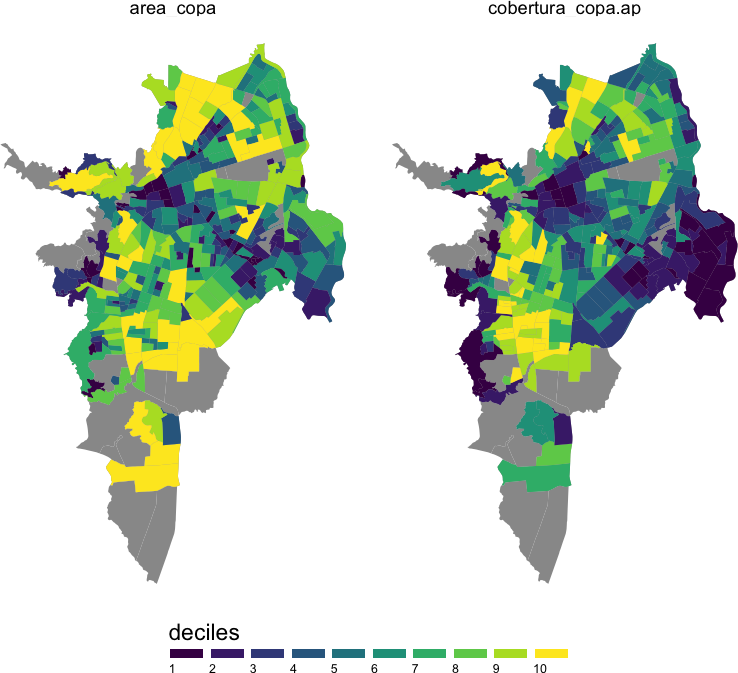
\includegraphics[width=1\linewidth]{tesis-unigis_files/figure-latex/mapa-copa-dep-1} \caption{Sectores urbanos de las variables dependientes sobre cobertura de copa}\label{fig:mapa-copa-dep}
\end{figure}

\subsubsection{Correlaciones y gráficos de dispersión entre
pares}\label{correlaciones-y-graficos-de-dispersion-entre-pares}

Para asegurarnos de que las variables no están correlacionadas entre si,
usaremos los coeficientes de correlación de Pearson, usado para detectar
relaciones lineales, usualmente en variables con distribución normal, y
el coeficiente de Spearman para detectar relaciones en variables con
otras distribuciones o que exhiben relaciones no lineales. Para tener
una idea más amplia sobre esa relación que expresan los coeficiente de
correlación se incluyen gráficas de dispersión entre las variables
independientes, y con las dependientes.

En la figura \ref{fig:bivar-poblacion-abs} se explora las relaciones
entre las variables de población en las unidades originales de los datos
(número de personas); la matriz triangular superior muestra los
coeficientes de correlación de Pearson, la diagonal contiene el
histogram de frecuencias de la variable y la matriz triangular inferior
muestra un gráfico de dispersión y la línea de tendencia usando un
modelo lineal entre cada par de variables. Es notoria la alta
correlación entre tener ningún estudio y tener alguna limitación física
(0.88); pertenecer a una comunidad afrodescendiente y carecer de
estudios (0.92) o ser afrodescendiente y tener alguna limitación (0.88).
Esto representa una suma de condiciones desfavorables relacionadas entre
sí, que desde el punta del vista del modelo sólo podrán ser
representadas por una de las variables, la que mejor se relacione con la
cobertura de copa y evitar así colinealidad entre los predictores.

\begin{figure}
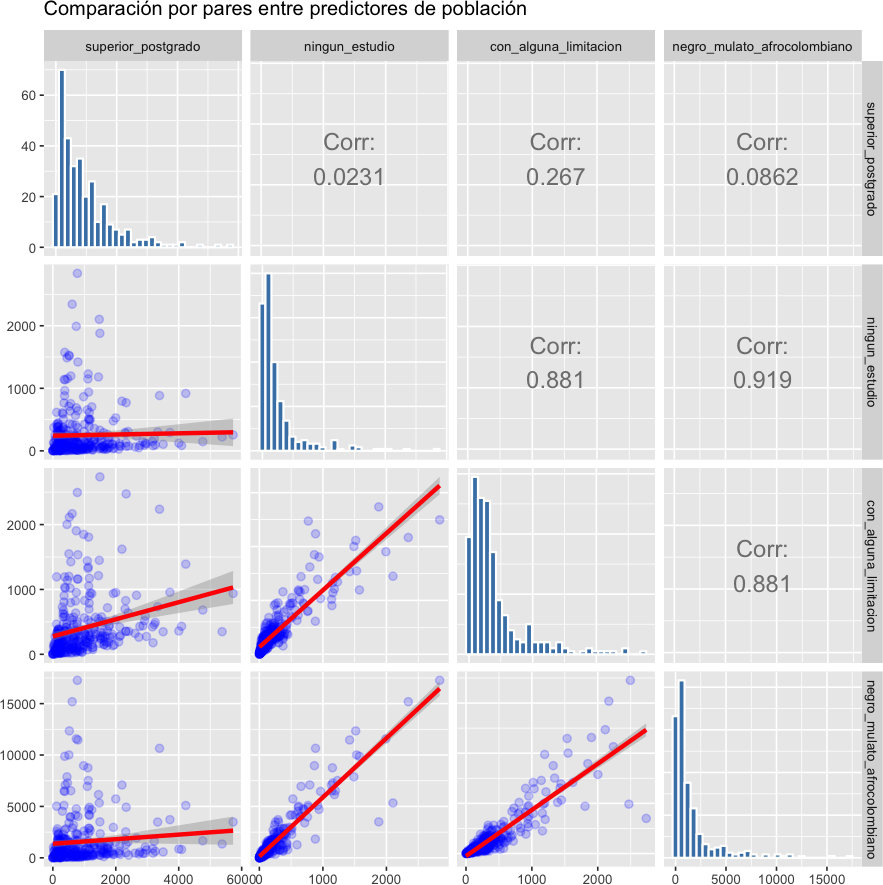
\includegraphics[width=1\linewidth]{tesis-unigis_files/figure-latex/bivar-poblacion-abs-1} \caption{Comparación por pares entre predictores de población}\label{fig:bivar-poblacion-abs}
\end{figure}

Cuando realizamos la misma comparación entre las variables porcentuales
(más la densidad poblacional) se observan patrones similares(ver figura
\ref{fig:bivar-poblacion-mod}): existe una alta correlación negativa
entre el porcentaje de población afro de un sector y la tenencia de
estudios superiores (-0.71), una fuerte asociación positiva entre el
porcentaje de personas afro de un sector y el porcentaje de personas que
carecen de estudios (0.68). También hay una fuerte relación inversa
entre el porcentaje de personas de un sector sin estudios y el
porcentaje de ellos que tiene estudios superiores (-0.8). Estas
variables evitaremos usarlas como predictores en una misma formulación
para no sesgar la estimación con problemas de colinealidad. Existe
también una asociación, no tan fuerte pero importante, entre la densidad
de población y sectores con mayor porcentaje de personas afro (0.47) y
una asociación negativa entre la densidad de población y el porcentaje
de personas con estudios superiores (-0.51). Estos resultados hablan de
una concentración de condiciones desfavorables para la población,
posiblemente acompañado de una segregación racial alta.

\begin{figure}
\includegraphics[width=1\linewidth]{tesis-unigis_files/figure-latex/bivar-poblacion-mod-1} \caption{Comparación por pares entre predictores de población porcentuales}\label{fig:bivar-poblacion-mod}
\end{figure}

Para completar la inspección de las relaciones entre predictores la
figura \ref{fig:bivar-poblacion-mod-abs} muestra la relación entre las
variables provistas en por el censo de población en unidades de personas
y las versiones porcentuales que calculamos. El número en el recuadro de
cada subgráfica es el coeficiente de correlación de Pearson. Aunque
procuraremos incluir cada una de las condiciones evitando redundar al
incluir la misma variable en sus dos versiones en un mismo modelo, es
interesante que la división entre el número de personas totales del
sector atenúa la correlación entre la variable observada y su
contraparte porcentual.

\begin{figure}
\includegraphics[width=1\linewidth]{tesis-unigis_files/figure-latex/bivar-poblacion-mod-abs-1} \caption{Comparación por pares entre predictores de población porcentuales y predictores en unidades de personas}\label{fig:bivar-poblacion-mod-abs}
\end{figure}

Ya que hemos explorado visualmente la dispersión entre los datos crudos,
podemos usar forma resumida, usando gráficos de azulejos o de matriz
para consultar la intensidad de estas relaciones, no solo las lineales
que revela el coeficiente de Pearson, sino usando el coeficiente de
Spearman. La figura @ref() sintetiza las relaciones lineales entre las
variables dependientes, mientras que la figura @ref() lo hace para las
no lineales.

\begin{figure}
\includegraphics[width=1\linewidth]{tesis-unigis_files/figure-latex/tile-poblacion-pearson-1} \caption{Coeficiente Pearson entre varibles de población}\label{fig:tile-poblacion-pearson}
\end{figure}

\begin{figure}
\includegraphics[width=1\linewidth]{tesis-unigis_files/figure-latex/tile-poblacion-spearman-1} \caption{Coeficiente Spearman entre varibles de población}\label{fig:tile-poblacion-spearman}
\end{figure}

Para seleccionar las variables que mejor predicen la cobertura de copa
aplicamos un procedimiento análogo al realizado con las variables
dependientes entre sí. Con base en los coeficientes de correlación de
Pearson (figura \ref{fig:tile-copa-poblacion-pearson}) y Spearman
(figura \ref{fig:tile-copa-poblacion-spearman}) entre las variables
dependientes e independientes, y teniendo en cuenta las restricciones de
colinealidad entre las variables dependientes, seleccionamos las
variables a usar en el modelo lineal.

Así pues, para el área de copa (\texttt{area\_copa}) los predictores
seleccionados
son\texttt{superior\_postgrado,\ densidad\_poblacion,\ con\_alguna\_limitacion.porcentaje,\ afro.porcentaje}
y para la cobertura de copa en área pública
(\texttt{cobertura\_copa.ap}) los predictores seleccionados
son\texttt{superior\_postgrado.porcentaje,\ densidad\_poblacion,\ con\_alguna\_limitacion.porcentaje,\ afro.porcentaje}

\begin{figure}
\includegraphics[width=1\linewidth]{tesis-unigis_files/figure-latex/tile-copa-poblacion-pearson-1} \caption{Coeficiente Pearson entre coberturas de copa y variables de población}\label{fig:tile-copa-poblacion-pearson}
\end{figure}

\begin{figure}
\includegraphics[width=1\linewidth]{tesis-unigis_files/figure-latex/tile-copa-poblacion-spearman-1} \caption{Coeficiente Spearman entre coberturas de copa y variables de población}\label{fig:tile-copa-poblacion-spearman}
\end{figure}

Se recomienda especificar correctamente los modelos lineales cuando
existen relaciones con correlaciones negativas, pues es posible que sea
mejor usar el inverso de la variable. Para probar si al hacerlo dichas
variables tienen incrementos en los coeficientes de correlación respecto
de las variables dependientes. Como se observa en las figuras
\ref{fig:duolin-poblacion-copa} y \ref{fig:duonolin-poblacioninv-copa}
las mejoras son solo en la varible de \texttt{afro.porcentaje.inv} en el
segundo dígito decimal. Como son tan pequeñas las diferencias opto por
no usar las variables transformdas por la funcion inversa pues esto
reduce el intervalo en que varian, reduciendo asi su poder explicativo.

\begin{figure}
\includegraphics[width=1\linewidth]{tesis-unigis_files/figure-latex/duolin-poblacion-copa-1} \caption{Gráficas de dispersión entre predictores de población y variables dependientes de la cobertura de copa (regresión lineal + coeficiente de Pearson)}\label{fig:duolin-poblacion-copa}
\end{figure}

\begin{figure}
\includegraphics[width=1\linewidth]{tesis-unigis_files/figure-latex/duonolin-poblacioninv-copa-1} \caption{Gráficas de dispersión entre predictores de población (usando el inverso de la variable con correlaciones negativas: $f(x)=\frac{1}{x+1}$) y las variables dependientes de la cobertura de copa ( regresión lineal  + coeficiente de Pearson)}\label{fig:duonolin-poblacioninv-copa}
\end{figure}

\subsubsection{Modelos de regresión
lineal}\label{modelos-de-regresion-lineal}

Antes ajustar los modelos suele ser común en los modelos de regresión
ajustar la distribución de las variables dependientes (y a veces las
independientes) por motivos teóricos usando transformaciones
logarítmicas o de raíz cuadra para eliminar no linealidades entre las
variables dependientes y las independientes, y reducir posibles
fenómenos de heterocedasticidad debido a estas no-linealidades.
Siguiendo el ejemplo, ajustaremos 5 modelos: uno por cada variable
dependiente en sus tres versiones, sin transforma, con una tranformacion
logaritmica (exepto para la cobertura\_copa.ap pues por tener valores ya
entre {[}0,1{]} produce valores negativos) y otra de la raiz cuadra.

Los histogramas de las variables dependientes tranformadas se muestran
en la figura \ref{fig:hist-copa-trnsf}.

\begin{figure}
\includegraphics[width=1\linewidth]{tesis-unigis_files/figure-latex/hist-copa-trnsf-1} \caption{Histogramas de las variables de cobertura de copa transformadas}\label{fig:hist-copa-trnsf}
\end{figure}

Las mejoras sobre el modelo de regresión que puedan hacer estas
transformaciones pueden apreciarse en los gráficos de dispersión de las
variables independientes transformadas vs.~las dependientes o/y en los
coeficientes de correlación de Pearson. Como se observa en las figuras
\ref{fig:duolin-poblacion-copa-trnsf} y
\ref{fig:duolin-poblacion-cob-trnsf} hay leves mejoras al aplicar las
transformaciones.

\begin{figure}
\includegraphics[width=1\linewidth]{tesis-unigis_files/figure-latex/duolin-poblacion-copa-trnsf-1} \caption{Gráficas de dispersión entre predictores de población y variables dependientes de la área de copa transformdas (regresión lineal + coeficiente de Pearson)}\label{fig:duolin-poblacion-copa-trnsf}
\end{figure}

\begin{figure}
\includegraphics[width=1\linewidth]{tesis-unigis_files/figure-latex/duolin-poblacion-cob-trnsf-1} \caption{Gráficas de dispersión entre predictores de población y variables dependientes de la cobertura de copa transformdas (regresión lineal + coeficiente de Pearson)}\label{fig:duolin-poblacion-cob-trnsf}
\end{figure}

También es sabido que dividir o multiplicar por alguna constante no
tiene ningún efecto en la calidad de la estimación , pero sí sobre los
coeficientes de la regresión. Esto suele ser sensible a la hora de
interpretar los cambios marginales de cada una de las variables
independientes y su efecto sobre la variable dependiente. Sin embargo,
lo que interesa para este estudio no es la interpretación de esos cambio
sino la importancia relativa de cada variable y comparar los cambios de
los coeficientes de regresión para el ajuste de cada modelo y/o las
mejoras que pueda operar un modelos autorregresivo en caso de encontrase
autocorrelación en los residuos de la regresión lineal. Por esta razón,
normalizar los valores puede ser una ventaja pues mantiene los
coeficiente mejor acotados. La normalización se aplica posterior a las
transformaciones propuestas y se realiza dividiendo por el máximo valor
de los datos de cada variable para mantener valores en el intervalo
{[}0,1{]}, dado que los valores son todos iguales o mayores que 0.

Al aplicar test para verificar que las condiciones de un buen ajuste (no
hay sesgos en el estimador o una mala especificación del modelo) de un
modelo lineal se cumplen:

\begin{itemize}
\tightlist
\item
  La media de los residuos es 0 o muy cercana.
\item
  La distribución de los residuos es normal.
\item
  Los residuos muestran homocedasticidad (la varianza es constante)
\end{itemize}

Para verificar la normalidad de los residuos usaremos el test de
Shapiro--Wilk \citep[ ]{shapiro1965analysis} y para la verificar si
existe homocedasticidad el test de Breusch--Pagan
\citep{breusch1979simple}. Además se acompaña de gráficas de diagnóstico
de los resultados de cada modelo. El siguiente código en \textbf{R} crea
las 5 regresiones lineales propuestas y se resumen en la la tablas
\ref{tab:comp-lmcopa} y \ref{tab:comp-lmcopaap}

\begin{Shaded}
\begin{Highlighting}[]
\NormalTok{dependiente <-}\StringTok{ "area_copa"}
\NormalTok{independientes <-}\StringTok{ }\NormalTok{indep.poblacion.copa.sel}
\NormalTok{var_names <-}\StringTok{ }\KeywordTok{c}\NormalTok{(dependiente, }\KeywordTok{names}\NormalTok{(regresion.arboles[, independientes]))}
\NormalTok{regresion.arboles.mn <-}\StringTok{ }\KeywordTok{max_nomalization}\NormalTok{(regresion.arboles, var_names)}
\NormalTok{lm.mn.area_copa.sel <-}\StringTok{ }\KeywordTok{crear_lm_from_df}\NormalTok{(regresion.arboles.mn)}
\NormalTok{sm <-}\StringTok{ }\KeywordTok{summary}\NormalTok{(lm.mn.area_copa.sel)}
\NormalTok{sm}
\end{Highlighting}
\end{Shaded}

\begin{verbatim}
## 
## Call:
## lm(formula = form, data = df)
## 
## Residuals:
##      Min       1Q   Median       3Q      Max 
## -0.24268 -0.05887 -0.01648  0.03275  0.75376 
## 
## Coefficients:
##                                      Estimate Std. Error t value Pr(>|t|)
## (Intercept)                           0.10059    0.02129   4.725 3.45e-06
## superior_postgrado.mxn                0.61703    0.03751  16.450  < 2e-16
## densidad_poblacion.mxn               -0.25404    0.03354  -7.574 3.94e-13
## con_alguna_limitacion.porcentaje.mxn -0.01734    0.04215  -0.411    0.681
## afro.porcentaje.mxn                   0.04459    0.03494   1.276    0.203
##                                         
## (Intercept)                          ***
## superior_postgrado.mxn               ***
## densidad_poblacion.mxn               ***
## con_alguna_limitacion.porcentaje.mxn    
## afro.porcentaje.mxn                     
## ---
## Signif. codes:  0 '***' 0.001 '**' 0.01 '*' 0.05 '.' 0.1 ' ' 1
## 
## Residual standard error: 0.1036 on 319 degrees of freedom
## Multiple R-squared:  0.5378, Adjusted R-squared:  0.532 
## F-statistic: 92.78 on 4 and 319 DF,  p-value: < 2.2e-16
\end{verbatim}

\begin{Shaded}
\begin{Highlighting}[]
\NormalTok{dependiente <-}\StringTok{ "log.area_copa"}
\NormalTok{independientes <-}\StringTok{ }\NormalTok{indep.poblacion.copa.sel}
\NormalTok{var_names <-}\StringTok{ }\KeywordTok{c}\NormalTok{(dependiente, }\KeywordTok{names}\NormalTok{(regresion.arboles[, independientes]))}
\NormalTok{regresion.arboles.mn <-}\StringTok{ }\KeywordTok{max_nomalization}\NormalTok{(regresion.arboles, var_names)}
\NormalTok{lm.mxn.log.area_copa.sel <-}\StringTok{ }\KeywordTok{crear_lm_from_df}\NormalTok{(regresion.arboles.mn)}
\NormalTok{modelo <-}\StringTok{ }\KeywordTok{crear_lm_from_df}\NormalTok{(regresion.arboles.mn)}
\NormalTok{sm <-}\StringTok{ }\KeywordTok{summary}\NormalTok{(lm.mxn.log.area_copa.sel)}
\NormalTok{sm}
\end{Highlighting}
\end{Shaded}

\begin{verbatim}
## 
## Call:
## lm(formula = form, data = df)
## 
## Residuals:
##       Min        1Q    Median        3Q       Max 
## -0.209393 -0.034801  0.000263  0.043219  0.180274 
## 
## Coefficients:
##                                      Estimate Std. Error t value Pr(>|t|)
## (Intercept)                           0.78745    0.01301  60.539  < 2e-16
## superior_postgrado.mxn                0.38208    0.02292  16.671  < 2e-16
## densidad_poblacion.mxn               -0.16544    0.02049  -8.073 1.42e-14
## con_alguna_limitacion.porcentaje.mxn -0.05635    0.02575  -2.188   0.0294
## afro.porcentaje.mxn                   0.04423    0.02135   2.072   0.0391
##                                         
## (Intercept)                          ***
## superior_postgrado.mxn               ***
## densidad_poblacion.mxn               ***
## con_alguna_limitacion.porcentaje.mxn *  
## afro.porcentaje.mxn                  *  
## ---
## Signif. codes:  0 '***' 0.001 '**' 0.01 '*' 0.05 '.' 0.1 ' ' 1
## 
## Residual standard error: 0.06329 on 319 degrees of freedom
## Multiple R-squared:  0.556,  Adjusted R-squared:  0.5504 
## F-statistic: 99.86 on 4 and 319 DF,  p-value: < 2.2e-16
\end{verbatim}

\begin{Shaded}
\begin{Highlighting}[]
\NormalTok{dependiente <-}\StringTok{ "sqrt.area_copa"}
\NormalTok{independientes <-}\StringTok{ }\NormalTok{indep.poblacion.copa.sel}
\NormalTok{var_names <-}\StringTok{ }\KeywordTok{c}\NormalTok{(dependiente, }\KeywordTok{names}\NormalTok{(regresion.arboles[, independientes]))}
\NormalTok{regresion.arboles.mn <-}\StringTok{ }\KeywordTok{max_nomalization}\NormalTok{(regresion.arboles, var_names)}
\NormalTok{lm.mxn.sqrt.area_copa.sel <-}\StringTok{ }\KeywordTok{crear_lm_from_df}\NormalTok{(regresion.arboles.mn)}
\KeywordTok{summary}\NormalTok{(lm.mxn.sqrt.area_copa.sel)}
\end{Highlighting}
\end{Shaded}

\begin{verbatim}
## 
## Call:
## lm(formula = form, data = df)
## 
## Residuals:
##      Min       1Q   Median       3Q      Max 
## -0.28930 -0.07310 -0.01329  0.06219  0.60651 
## 
## Coefficients:
##                                      Estimate Std. Error t value Pr(>|t|)
## (Intercept)                           0.28925    0.02274  12.720   <2e-16
## superior_postgrado.mxn                0.75574    0.04007  18.862   <2e-16
## densidad_poblacion.mxn               -0.31411    0.03583  -8.768   <2e-16
## con_alguna_limitacion.porcentaje.mxn -0.04616    0.04502  -1.025    0.306
## afro.porcentaje.mxn                   0.05709    0.03732   1.530    0.127
##                                         
## (Intercept)                          ***
## superior_postgrado.mxn               ***
## densidad_poblacion.mxn               ***
## con_alguna_limitacion.porcentaje.mxn    
## afro.porcentaje.mxn                     
## ---
## Signif. codes:  0 '***' 0.001 '**' 0.01 '*' 0.05 '.' 0.1 ' ' 1
## 
## Residual standard error: 0.1107 on 319 degrees of freedom
## Multiple R-squared:  0.6089, Adjusted R-squared:  0.604 
## F-statistic: 124.2 on 4 and 319 DF,  p-value: < 2.2e-16
\end{verbatim}

Como se muestra en la tabla \ref{tab:comp-lmcopa}De las 3 formulaciones
de usadas para modelar el área de copa la que mejor ajuste obtuvo fue el
que transforma la variable dependiente usando la raíz cuadrada
(\texttt{log.area\_copa}). Aunque el modelo de \texttt{sqrt.area\_copa}
explica el 60\% de la variabilidad en los datos (Adjusted R-squared:
0.604), la versión logaritmica tiene un MSE y Akaike menor, y los
residuos son normales (el test Shapiro). Este modelo considera las
variables \texttt{superior\_postgrado} y \texttt{densidad\_poblacion}
como muy significativas, ambos con coeficientes obteniendo valores
consistentes con el signo de las correlaciones calculadas previamente en
análisis bivariado de la figura \ref{fig:duolin-poblacion-copa-trnsf}.

\begin{table}

\caption{\label{tab:comp-lmcopa}Resúmen ajuste modelos área copa preliminares}
\centering
\begin{tabular}[t]{l|r|r|r}
\hline
medidasfit & AC & Log(AC) & Sqrt(AC)\\
\hline
Shapiro-Wilk & 0.82608 & 0.99140 & 0.94358\\
\hline
SW p-value & 0.00000 & 0.05605 & 0.00000\\
\hline
Breusch-Pagan & 25.76218 & 12.02058 & 23.46806\\
\hline
BP p-value & 0.00004 & 0.01720 & 0.00010\\
\hline
Media Residuos & 0.00000 & 0.00000 & 0.00000\\
\hline
MSE & 0.01057 & 0.00394 & 0.01206\\
\hline
adj-Rsquare & 0.53196 & 0.55042 & 0.60400\\
\hline
AIC & -542.76569 & -862.01544 & -500.03911\\
\hline
Log likelihood & 277.38284 & 437.00772 & 256.01956\\
\hline
\end{tabular}
\end{table}

Los modelos del porcenataje de cobertura de copa son lo siguientes:

\begin{Shaded}
\begin{Highlighting}[]
\NormalTok{dependiente <-}\StringTok{ "cobertura_copa.ap"}
\NormalTok{independientes <-}\StringTok{ }\NormalTok{indep.poblacion.copa.ap.sel}
\NormalTok{var_names <-}\StringTok{ }\KeywordTok{c}\NormalTok{(dependiente, }\KeywordTok{names}\NormalTok{(regresion.arboles[, independientes]))}
\NormalTok{regresion.arboles.mn <-}\StringTok{ }\KeywordTok{max_nomalization}\NormalTok{(regresion.arboles, var_names)}
\NormalTok{lm.mxn.cobertura_copa.ap <-}\StringTok{ }\KeywordTok{crear_lm_from_df}\NormalTok{(regresion.arboles.mn)}
\NormalTok{sm <-}\StringTok{ }\KeywordTok{summary}\NormalTok{(lm.mxn.cobertura_copa.ap)}
\NormalTok{sm}
\end{Highlighting}
\end{Shaded}

\begin{verbatim}
## 
## Call:
## lm(formula = form, data = df)
## 
## Residuals:
##      Min       1Q   Median       3Q      Max 
## -0.28517 -0.05598 -0.01502  0.04070  0.65940 
## 
## Coefficients:
##                                      Estimate Std. Error t value Pr(>|t|)
## (Intercept)                          0.007612   0.033577   0.227    0.821
## superior_postgrado.porcentaje.mxn    0.387778   0.032525  11.923   <2e-16
## densidad_poblacion.mxn               0.052744   0.034832   1.514    0.131
## con_alguna_limitacion.porcentaje.mxn 0.053220   0.044071   1.208    0.228
## afro.porcentaje.mxn                  0.005960   0.040894   0.146    0.884
##                                         
## (Intercept)                             
## superior_postgrado.porcentaje.mxn    ***
## densidad_poblacion.mxn                  
## con_alguna_limitacion.porcentaje.mxn    
## afro.porcentaje.mxn                     
## ---
## Signif. codes:  0 '***' 0.001 '**' 0.01 '*' 0.05 '.' 0.1 ' ' 1
## 
## Residual standard error: 0.105 on 319 degrees of freedom
## Multiple R-squared:  0.4644, Adjusted R-squared:  0.4576 
## F-statistic: 69.14 on 4 and 319 DF,  p-value: < 2.2e-16
\end{verbatim}

\begin{Shaded}
\begin{Highlighting}[]
\NormalTok{dependiente <-}\StringTok{ "sqrt.cobertura_copa.ap"}
\NormalTok{independientes <-}\StringTok{ }\NormalTok{indep.poblacion.copa.ap.sel}
\NormalTok{var_names <-}\StringTok{ }\KeywordTok{c}\NormalTok{(dependiente, }\KeywordTok{names}\NormalTok{(regresion.arboles[, independientes]))}
\NormalTok{regresion.arboles.mn <-}\StringTok{ }\KeywordTok{max_nomalization}\NormalTok{(regresion.arboles, var_names)}
\NormalTok{lm.mxn.sqrt.cobertura_copa.ap <-}\StringTok{ }\KeywordTok{crear_lm_from_df}\NormalTok{(regresion.arboles.mn)}
\NormalTok{sm <-}\StringTok{ }\KeywordTok{summary}\NormalTok{(lm.mxn.sqrt.cobertura_copa.ap)}
\NormalTok{sm}
\end{Highlighting}
\end{Shaded}

\begin{verbatim}
## 
## Call:
## lm(formula = form, data = df)
## 
## Residuals:
##      Min       1Q   Median       3Q      Max 
## -0.38864 -0.06666 -0.00395  0.06375  0.42095 
## 
## Coefficients:
##                                       Estimate Std. Error t value Pr(>|t|)
## (Intercept)                           0.201407   0.036441   5.527 6.78e-08
## superior_postgrado.porcentaje.mxn     0.444226   0.035300  12.584  < 2e-16
## densidad_poblacion.mxn                0.100341   0.037804   2.654  0.00835
## con_alguna_limitacion.porcentaje.mxn  0.033052   0.047831   0.691  0.49006
## afro.porcentaje.mxn                  -0.003885   0.044384  -0.088  0.93031
##                                         
## (Intercept)                          ***
## superior_postgrado.porcentaje.mxn    ***
## densidad_poblacion.mxn               ** 
## con_alguna_limitacion.porcentaje.mxn    
## afro.porcentaje.mxn                     
## ---
## Signif. codes:  0 '***' 0.001 '**' 0.01 '*' 0.05 '.' 0.1 ' ' 1
## 
## Residual standard error: 0.1139 on 319 degrees of freedom
## Multiple R-squared:  0.4922, Adjusted R-squared:  0.4858 
## F-statistic:  77.3 on 4 and 319 DF,  p-value: < 2.2e-16
\end{verbatim}

Como se observa en la tabla \ref{tab:comp-lmcopaap} el porcentaje de
cobertura copa en el área pública, el mejor ajuste se obtuvo con la
variable sin transformación \texttt{cobertura\_copa.ap}. Este modelo
considera que solo la variable \texttt{superior\_postgrado.porcentaje}
como muy significativas, y explica casi el 46\% de la variabilidad
(Adjusted R-squared: 0.4576384) con MSE y Akaike menores. El coeficiente
de la densidad de población obtiene un valor positivo y poco
significativo, contrario al signo de la correlación obtenida en el
análisis bivariado de la figura \ref{fig:duolin-poblacion-cob-trnsf},
por lo que es descartado.

\begin{table}

\caption{\label{tab:comp-lmcopaap}Resúmen ajuste de porcentaje de cobertura de copa preliminares}
\centering
\begin{tabular}[t]{l|r|r}
\hline
medidasfit & \%CC & Sqrt(\%CC)\\
\hline
Shapiro-Wilk & 0.89928 & 0.98221\\
\hline
SW p-value & 0.00000 & 0.00048\\
\hline
Breusch-Pagan & 18.48790 & 12.36483\\
\hline
BP p-value & 0.00099 & 0.01483\\
\hline
Media Residuos & 0.00000 & 0.00000\\
\hline
MSE & 0.01085 & 0.01278\\
\hline
adj-Rsquare & 0.45764 & 0.48584\\
\hline
AIC & -534.19892 & -481.14452\\
\hline
Log likelihood & 273.09946 & 246.57226\\
\hline
\end{tabular}
\end{table}

Reduzcamos ambos modelos eliminando las variables no significativas.
Para el mejor modelo del área de copa el siguiente código realiza el
trabajo resumir los resultados en gráficas diagnósticas y los tests de
normalidad y homocedasticidad en la tabla \ref{tab:fitlm-copa-best}.

\begin{Shaded}
\begin{Highlighting}[]
\NormalTok{dependiente <-}\StringTok{ "log.area_copa"}
\NormalTok{independientes <-}\StringTok{ }\KeywordTok{c}\NormalTok{(}\StringTok{"superior_postgrado"}\NormalTok{, }\StringTok{"densidad_poblacion"}\NormalTok{)}
\NormalTok{var_names <-}\StringTok{ }\KeywordTok{c}\NormalTok{(dependiente, }\KeywordTok{names}\NormalTok{(regresion.arboles[, independientes]))}
\NormalTok{regresion.arboles.mn <-}\StringTok{ }\KeywordTok{max_nomalization}\NormalTok{(regresion.arboles, var_names)}
\NormalTok{lm.best.area_copa <-}\StringTok{ }\KeywordTok{lm}\NormalTok{(log.area_copa.mxn }\OperatorTok{~}\StringTok{ }\NormalTok{superior_postgrado.mxn }\OperatorTok{+}\StringTok{ }\NormalTok{densidad_poblacion.mxn, }
    \DataTypeTok{data =}\NormalTok{ regresion.arboles.mn)}
\NormalTok{sm <-}\StringTok{ }\KeywordTok{summary}\NormalTok{(lm.best.area_copa)}
\NormalTok{sm}
\end{Highlighting}
\end{Shaded}

\begin{verbatim}
## 
## Call:
## lm(formula = log.area_copa.mxn ~ superior_postgrado.mxn + densidad_poblacion.mxn, 
##     data = regresion.arboles.mn)
## 
## Residuals:
##       Min        1Q    Median        3Q       Max 
## -0.228080 -0.034443  0.003531  0.044043  0.191950 
## 
## Coefficients:
##                         Estimate Std. Error t value Pr(>|t|)    
## (Intercept)             0.773649   0.007707 100.380   <2e-16 ***
## superior_postgrado.mxn  0.373575   0.021809  17.130   <2e-16 ***
## densidad_poblacion.mxn -0.158838   0.017814  -8.917   <2e-16 ***
## ---
## Signif. codes:  0 '***' 0.001 '**' 0.01 '*' 0.05 '.' 0.1 ' ' 1
## 
## Residual standard error: 0.06378 on 321 degrees of freedom
## Multiple R-squared:  0.5463, Adjusted R-squared:  0.5435 
## F-statistic: 193.3 on 2 and 321 DF,  p-value: < 2.2e-16
\end{verbatim}

\begin{figure}
\includegraphics[width=1\linewidth]{tesis-unigis_files/figure-latex/diagn-best-lm-areacopa-1} \caption{Gráficas diagnósticas para el análisis de regresión lineal del área de copa}\label{fig:diagn-best-lm-areacopa}
\end{figure}

Los resultados de los tests (tabla \ref{tab:fitlm-copa-best}) rechazan
que los residuos sean normales, pero la varianza pasa el test
Breusch-Pagan de homocedasticidad. Es posibles que los estimadores sean
ineficientes y que existan efecto no considerados en el modelo dada la
no normalidad de los residuos. Las gráficas diagnosticas (figura
\ref{fig:diagn-best-lm-areacopa}) muestran que existe no linealidades en
los residuos, pues se observa como la linea de tendencia hace curvas
respecto de la horizontal. Para probar si es posible tener un modelo
mejor especificado se introduce en la sección
\protect\hyperlink{geostat}{análisis geoestadisticos} basados en la
autocorrelación espacial.

\begin{table}

\caption{\label{tab:fitlm-copa-best}Resúmen ajuste OLS: log(area copa)}
\centering
\begin{tabular}[t]{l|r}
\hline
medidasfit & Area Copa\\
\hline
Shapiro-Wilk & 0.98764\\
\hline
SW p-value & 0.00732\\
\hline
Breusch-Pagan & 5.24932\\
\hline
BP p-value & 0.07246\\
\hline
Media Residuos & 0.00000\\
\hline
MSE & 0.00403\\
\hline
adj-Rsquare & 0.54348\\
\hline
AIC & -859.02772\\
\hline
Log likelihood & 433.51386\\
\hline
\end{tabular}
\end{table}

El mismo procedimiento lo aplicamos para el mejor modelo de cobertura de
copa. El siguiente código construye el modelo y realiza los test
descritos anteriormente.

\begin{Shaded}
\begin{Highlighting}[]
\NormalTok{dependiente <-}\StringTok{ "cobertura_copa.ap"}
\NormalTok{independientes <-}\StringTok{ }\KeywordTok{c}\NormalTok{(}\StringTok{"superior_postgrado.porcentaje"}\NormalTok{)}
\CommentTok{# max normalizado}
\NormalTok{var_names <-}\StringTok{ }\KeywordTok{c}\NormalTok{(dependiente, independientes)}
\NormalTok{regresion.arboles.mn <-}\StringTok{ }\KeywordTok{max_nomalization}\NormalTok{(regresion.arboles, var_names)}
\NormalTok{lm.best.cobertura.ap <-}\StringTok{ }\KeywordTok{lm}\NormalTok{(cobertura_copa.ap.mxn }\OperatorTok{~}\StringTok{ }\NormalTok{superior_postgrado.porcentaje.mxn, }
    \DataTypeTok{data =}\NormalTok{ regresion.arboles.mn)}
\NormalTok{sm <-}\StringTok{ }\KeywordTok{summary}\NormalTok{(lm.best.cobertura.ap)}
\NormalTok{sm}
\end{Highlighting}
\end{Shaded}

\begin{verbatim}
## 
## Call:
## lm(formula = cobertura_copa.ap.mxn ~ superior_postgrado.porcentaje.mxn, 
##     data = regresion.arboles.mn)
## 
## Residuals:
##      Min       1Q   Median       3Q      Max 
## -0.29895 -0.05645 -0.01560  0.04094  0.66402 
## 
## Coefficients:
##                                   Estimate Std. Error t value Pr(>|t|)    
## (Intercept)                       0.065794   0.009627   6.835 4.13e-11 ***
## superior_postgrado.porcentaje.mxn 0.350233   0.021283  16.456  < 2e-16 ***
## ---
## Signif. codes:  0 '***' 0.001 '**' 0.01 '*' 0.05 '.' 0.1 ' ' 1
## 
## Residual standard error: 0.1052 on 322 degrees of freedom
## Multiple R-squared:  0.4568, Adjusted R-squared:  0.4551 
## F-statistic: 270.8 on 1 and 322 DF,  p-value: < 2.2e-16
\end{verbatim}

\begin{figure}
\includegraphics[width=1\linewidth]{tesis-unigis_files/figure-latex/diagn-best-lm-copaap-1} \caption{Gráficas diagnósticas para el análisis de regresión lineal del porcentaje de cobertura de copa}\label{fig:diagn-best-lm-copaap}
\end{figure}

\begin{table}

\caption{\label{tab:fitlm-copaap-best}Resúmen ajuste OLS: cobertura copa.ap}
\centering
\begin{tabular}[t]{l|r}
\hline
medidasfit & \%Cobertura de Copa\\
\hline
Shapiro-Wilk & 0.90492\\
\hline
SW p-value & 0.00000\\
\hline
Breusch-Pagan & 16.82734\\
\hline
BP p-value & 0.00004\\
\hline
Media Residuos & 0.00000\\
\hline
MSE & 0.01100\\
\hline
adj-Rsquare & 0.45512\\
\hline
AIC & -535.66435\\
\hline
Log likelihood & 270.83218\\
\hline
\end{tabular}
\end{table}

Los resultados de los tests rechazan que los residuos sean normales y
que la varianza sea constante (tabla \ref{tab:fitlm-copaap-best}), sin
embargo, es notorio el aumento de la varianza con el aumento de los
valores ajustados; la curva de tendencia de los residuos vs.~los valores
ajustados sigue una linea de tendencia que se distancia de la horizontal
confirmando la heterocedasticidad de los residuos (figura
\ref{fig:diagn-best-lm-copaap}). Igualmente veremos si la introducción
de elementos de la teoría geoestadística permite mejorar la
especificación del modelo.

\subsubsection{Introducción de dimensiones no poblacionales al modelo
lineal}\label{introduccion-de-dimensiones-no-poblacionales-al-modelo-lineal}

Para la inclusión de otras variables agregadas por sector urbano
aplicamos el procedimiento realizado para la selección de las variables
de población usando como criterio la inclusión de variables con
coeficientes de correlación que muestren una asociación fuerte con las
variables de cobertura de copa. Las figuras
\ref{fig:tile-prediosev-pearson} y \ref{fig:tile-prediosev-spearman} se
ven los coeficientes de Pearson y Spearman, respectivamente, entre las
variables sobre el uso los predios, tipo de viviendas y área (y
porcentaje) de espacios verdes en cada sector urbano. Como se observa,
existe una fuerte (perfecta) asociación negativa entre el porcentaje de
casas y apartamentos, lo que obliga a solo escoger una de las dos en
caso de haber una fuerte relación entre alguna de ellas con las
variables de cobertura de copa. También hay una fuerte asociación
positiva entre el área de espacios verdes y el porcentaje de área de
espacio verdes en un sector urbano. Como mencionamos antes solo
incluiremos una de las dos en caso de que ambas resulten fuertemente
asociadas con las variables dependientes.

\begin{figure}
\includegraphics[width=1\linewidth]{tesis-unigis_files/figure-latex/tile-prediosev-pearson-1} \caption{Coeficiente Pearson entre variables de uso de los predios y espacios verdes en los sectores urbanos}\label{fig:tile-prediosev-pearson}
\end{figure}

\begin{figure}
\includegraphics[width=1\linewidth]{tesis-unigis_files/figure-latex/tile-prediosev-spearman-1} \caption{Coeficiente Pearson entre variables de uso de los predios y espacios verdes en los sectores urbanos}\label{fig:tile-prediosev-spearman}
\end{figure}

Las figuras \ref{fig:tile-copa-prediosev-pearson} y
\ref{fig:tile-copa-prediosev-spearman} muestran la correlación entre las
potenciales nuevas variables a incluir en el modelo y las variables
dependientes de cobertura y área de copa. Para el área de copa se
seleccionan el área de espacios verdes (\texttt{area\_ep}) y el
porcentaje de viviendas tipo cuarto (\texttt{cuarto.porcentaje}). Para
el modelo de porcentaje de cobertura de se seleccionan
\texttt{apartamento.porcentaje}, \texttt{cuarto.porcentaje} y
\texttt{area\_ep.porcentaje}.

\begin{figure}
\includegraphics[width=1\linewidth]{tesis-unigis_files/figure-latex/tile-copa-prediosev-pearson-1} \caption{Coeficiente Pearson entre coberturas de copa y variables de predios y EV}\label{fig:tile-copa-prediosev-pearson}
\end{figure}

\begin{figure}
\includegraphics[width=1\linewidth]{tesis-unigis_files/figure-latex/tile-copa-prediosev-spearman-1} \caption{Coeficiente Pearson entre coberturas de copa y variables de predios y EV}\label{fig:tile-copa-prediosev-spearman}
\end{figure}

La nueva formulación del modelo de área de copa obtiene los siguientes
resultados:

\begin{Shaded}
\begin{Highlighting}[]
\CommentTok{# introducimos las varibles nuevas}
\NormalTok{dependiente <-}\StringTok{ "log.area_copa"}
\NormalTok{independientes <-}\StringTok{ }\KeywordTok{c}\NormalTok{(}\StringTok{"superior_postgrado"}\NormalTok{, }\StringTok{"densidad_poblacion"}\NormalTok{, indep.predios.copa.sel)}
\CommentTok{# max normalizado}
\NormalTok{var_names <-}\StringTok{ }\KeywordTok{c}\NormalTok{(dependiente, }\KeywordTok{names}\NormalTok{(regresion.arboles[, independientes]))}
\NormalTok{regresion.arboles.mn <-}\StringTok{ }\KeywordTok{max_nomalization}\NormalTok{(regresion.arboles, var_names)}
\NormalTok{lm.mod.area_copa <-}\StringTok{ }\KeywordTok{lm}\NormalTok{(log.area_copa.mxn }\OperatorTok{~}\StringTok{ }\NormalTok{superior_postgrado.mxn }\OperatorTok{+}\StringTok{ }\NormalTok{densidad_poblacion.mxn }\OperatorTok{+}\StringTok{ }
\StringTok{    }\NormalTok{cuarto.porcentaje.mxn }\OperatorTok{+}\StringTok{ }\NormalTok{area_ep.mxn, }\DataTypeTok{data =}\NormalTok{ regresion.arboles.mn)}
\NormalTok{sm <-}\StringTok{ }\KeywordTok{summary}\NormalTok{(lm.mod.area_copa)}
\NormalTok{sm}
\end{Highlighting}
\end{Shaded}

\begin{verbatim}
## 
## Call:
## lm(formula = log.area_copa.mxn ~ superior_postgrado.mxn + densidad_poblacion.mxn + 
##     cuarto.porcentaje.mxn + area_ep.mxn, data = regresion.arboles.mn)
## 
## Residuals:
##       Min        1Q    Median        3Q       Max 
## -0.219304 -0.030935  0.004071  0.041703  0.125492 
## 
## Coefficients:
##                         Estimate Std. Error t value Pr(>|t|)    
## (Intercept)             0.781751   0.008458  92.431  < 2e-16 ***
## superior_postgrado.mxn  0.309340   0.022118  13.986  < 2e-16 ***
## densidad_poblacion.mxn -0.146445   0.016984  -8.623 3.11e-16 ***
## cuarto.porcentaje.mxn  -0.149299   0.029954  -4.984 1.02e-06 ***
## area_ep.mxn             0.123103   0.026560   4.635 5.21e-06 ***
## ---
## Signif. codes:  0 '***' 0.001 '**' 0.01 '*' 0.05 '.' 0.1 ' ' 1
## 
## Residual standard error: 0.05922 on 319 degrees of freedom
## Multiple R-squared:  0.6113, Adjusted R-squared:  0.6064 
## F-statistic: 125.4 on 4 and 319 DF,  p-value: < 2.2e-16
\end{verbatim}

\begin{table}

\caption{\label{tab:comp-lmcopa-pob-mod}Comparación OLS para el área de copa (AC) con variables de población y con otras dimensiones}
\centering
\begin{tabular}[t]{l|r|r}
\hline
medidasfit & Log(AC)\textasciitilde{}pob & log(AC)\textasciitilde{}pob+otras\\
\hline
Shapiro-Wilk & 0.98764 & 0.97939\\
\hline
SW p-value & 0.00732 & 0.00013\\
\hline
Breusch-Pagan & 5.24932 & 6.70653\\
\hline
BP p-value & 0.07246 & 0.15223\\
\hline
Media Residuos & 0.00000 & 0.00000\\
\hline
MSE & 0.00403 & 0.00345\\
\hline
adj-Rsquare & 0.54348 & 0.60639\\
\hline
AIC & -859.02772 & -905.09560\\
\hline
Log likelihood & 433.51386 & 458.54780\\
\hline
\end{tabular}
\end{table}

Las variables introducidas tienen todas p-value significativos, y a
pesar de la inclusión de más términos al modelo existe una mejora en el
Criterio de Información de Akaike (baja de \(-859.0277185\) a
\(-905.0955982\)). Los resultados de los test evidencian que aunque hay
mejoras en Adjusted R-squared ( de \(0.5434765\) a \(0.6063903\)) y en
MSE (de \(0.0040304\) a \(0.0034533\)) sigue existiendo no normalidad en
los residuos y posibles no linealidades, como se observa también en las
gráficas diagnosticas de la regresión \ref{fig:diagn-mod-best-lm-copa}.

\begin{figure}
\includegraphics[width=1\linewidth]{tesis-unigis_files/figure-latex/diagn-mod-best-lm-copa-1} \caption{Gráficas diagnósticas para el análisis de regresión lineal de área de copa con los nuevos términos}\label{fig:diagn-mod-best-lm-copa}
\end{figure}

Para el caso del porcentaje de cobertura de copa los resultados
obtenidos con la introduccion de las nuevas varibles son los siguientes:

\begin{Shaded}
\begin{Highlighting}[]
\CommentTok{# coberbtura AP}
\NormalTok{dependiente <-}\StringTok{ "cobertura_copa.ap"}
\NormalTok{independientes <-}\StringTok{ }\KeywordTok{c}\NormalTok{(}\StringTok{"superior_postgrado.porcentaje"}\NormalTok{, indep.predios.copa.ap.sel)}
\CommentTok{# max normalizado}
\NormalTok{var_names <-}\StringTok{ }\KeywordTok{c}\NormalTok{(dependiente, independientes)}
\NormalTok{regresion.arboles.mn <-}\StringTok{ }\KeywordTok{max_nomalization}\NormalTok{(regresion.arboles, var_names)}
\NormalTok{lm.mod.cobertura.ap <-}\StringTok{ }\KeywordTok{lm}\NormalTok{(cobertura_copa.ap.mxn }\OperatorTok{~}\StringTok{ }\NormalTok{superior_postgrado.porcentaje.mxn }\OperatorTok{+}\StringTok{ }
\StringTok{    }\NormalTok{apartamento.porcentaje.mxn }\OperatorTok{+}\StringTok{ }\NormalTok{cuarto.porcentaje.mxn }\OperatorTok{+}\StringTok{ }\NormalTok{area_ep.porcentaje.mxn, }
    \DataTypeTok{data =}\NormalTok{ regresion.arboles.mn)}
\NormalTok{sm <-}\StringTok{ }\KeywordTok{summary}\NormalTok{(lm.mod.cobertura.ap)}
\NormalTok{sm}
\end{Highlighting}
\end{Shaded}

\begin{verbatim}
## 
## Call:
## lm(formula = cobertura_copa.ap.mxn ~ superior_postgrado.porcentaje.mxn + 
##     apartamento.porcentaje.mxn + cuarto.porcentaje.mxn + area_ep.porcentaje.mxn, 
##     data = regresion.arboles.mn)
## 
## Residuals:
##      Min       1Q   Median       3Q      Max 
## -0.29520 -0.05565 -0.00936  0.03833  0.65485 
## 
## Coefficients:
##                                   Estimate Std. Error t value Pr(>|t|)    
## (Intercept)                        0.08310    0.01664   4.995  9.7e-07 ***
## superior_postgrado.porcentaje.mxn  0.34914    0.02728  12.797  < 2e-16 ***
## apartamento.porcentaje.mxn        -0.03315    0.03408  -0.973    0.331    
## cuarto.porcentaje.mxn             -0.08121    0.05569  -1.458    0.146    
## area_ep.porcentaje.mxn             0.02887    0.03735   0.773    0.440    
## ---
## Signif. codes:  0 '***' 0.001 '**' 0.01 '*' 0.05 '.' 0.1 ' ' 1
## 
## Residual standard error: 0.1051 on 319 degrees of freedom
## Multiple R-squared:  0.4635, Adjusted R-squared:  0.4568 
## F-statistic: 68.91 on 4 and 319 DF,  p-value: < 2.2e-16
\end{verbatim}

\begin{table}

\caption{\label{tab:comp-lmcopaap-pob-mod}Comparación OLS para el porcentaje de cobertura de copa con variables de población y otras dimensiones}
\centering
\begin{tabular}[t]{l|r|r}
\hline
medidasfit & \%CC \textasciitilde{} pob & \%CC \textasciitilde{} pob+otras\\
\hline
Shapiro-Wilk & 0.90492 & 0.90720\\
\hline
SW p-value & 0.00000 & 0.00000\\
\hline
Breusch-Pagan & 16.82734 & 18.75791\\
\hline
BP p-value & 0.00004 & 0.00088\\
\hline
Media Residuos & 0.00000 & 0.00000\\
\hline
MSE & 0.01100 & 0.01087\\
\hline
adj-Rsquare & 0.45512 & 0.45681\\
\hline
AIC & -535.66435 & -533.70683\\
\hline
Log likelihood & 270.83218 & 272.85342\\
\hline
\end{tabular}
\end{table}

Las variables introducidas tienen todas p-value no significativos. La
inclusión de más términos al modelo empeoran el Criterio de Información
de Akaike (sube de \(-535.6643522\) a \(-533.7068318\)). Los resultados
de los test no dan evidencian de mejoras importantes en Adjusted
R-squared ( de \(0.4551186\) a \(0.456814\) ) o en MSE (de \(0.011002\)
a \(0.0108656\)). Sigue existiendo no normalidad en los residuos y
heterocedasticidad, como se verifica en las gráficas diagnosticas de la
regresión \ref{fig:diagn-mod-best-lm-copaap}.

\begin{figure}
\includegraphics[width=1\linewidth]{tesis-unigis_files/figure-latex/diagn-mod-best-lm-copaap-1} \caption{Gráficas diagnósticas para el análisis de regresión lineal de porcentaje de cobertura de copa con los nuevos términos}\label{fig:diagn-mod-best-lm-copaap}
\end{figure}

Finalmente presento los mapas de las variables dependientes de los 2
modelos seleccionados, comparandolas con el modelo ajustado y los
residuos de ajuste, con el finde observar donde se localizan los errores
en la predicción. La figura \ref{fig:mapas-lm-copa} corresponde al
ajuste del área de copa y la figura \ref{fig:mapas-lm-copaap} al
porcentaje de la cobertura de copa.

\begin{figure}
\includegraphics[width=1\linewidth]{tesis-unigis_files/figure-latex/mapas-lm-copa-1} \caption{Variable dependiente, valor ajsutado por el modelo y residuos del OLS para log.area copa normalizada}\label{fig:mapas-lm-copa}
\end{figure}

\begin{figure}
\includegraphics[width=1\linewidth]{tesis-unigis_files/figure-latex/mapas-lm-copaap-1} \caption{Variable dependiente, valor ajsutado por el modelo y residuos del OLS para cobertura copa.ap normalizada}\label{fig:mapas-lm-copaap}
\end{figure}

\subsection{Acceso a espacios verdes}\label{acceso-a-espacios-verdes}

\begin{figure}
\includegraphics[width=1\linewidth]{tesis-unigis_files/figure-latex/mapa-dependienteEV-all-1} \caption{Metricas de acceso a espacio verdes}\label{fig:mapa-dependienteEV-all}
\end{figure}

En el caso de los EV contamos con una gran variedad de medidas sobre el
acceso en relación con la distancia, el área disponible y diferentes
formulaciones para aproximarse al concepto de acceso a un servicio
ambiental (Figura \ref{fig:mapa-dependienteEV-all}). Para acotar el
alcance de este trabajo, nos concentramos en dos métricas: el porcentaje
de área de espacio verde de un sector censal
(\texttt{area\_ep.porcentaje}), para aproximarse desde la idea de los
beneficios principalmente a nivel local, y la razón área disponible
distancia (\texttt{ia.areas.dist}), que tiende a formar agrupaciones de
SU al rededor de las sectore donde se ubican espacios verdes, ya sea por
número o por tamaño, que contemplan el fenómeno del acceso o beneficio
como un proceso acotado por la distancia escogida de 1 kilómetro como
radio de búsqueda; considerándola una distancia caminable para viajar en
una ciudad como Cali. (Figura \ref{fig:mapa-dependienteEV-sel})

\begin{figure}
\includegraphics[width=1\linewidth]{tesis-unigis_files/figure-latex/mapa-dependienteEV-sel-1} \caption{Metricas de acceso a espacio verdes seleccionadas}\label{fig:mapa-dependienteEV-sel}
\end{figure}

\subsubsection{Correlaciones y distribuciones
bivaridas}\label{correlaciones-y-distribuciones-bivaridas}

Las variables de población y su correlación con los indicadores de
acceso seleccionados nos sirven para seleccionar una vez más las
variables independientes para usar en los modelos de regresión lineal.
Las figuras \ref{fig:tile-ev-poblacion-pearson} y
\ref{fig:tile-ev-poblacion-spearman} resumen los resultados del cálculo
de los coeficientes de Pearson y Spearman respectivamente. Como se
observa, esta relación es muy débil, y en todos las variables (y para
ambos coeficientes de correlación) es inferior a 0.3, un valor
considerado muy bajo para incluir alguna de estas variables para que
tenga éxito una aproximación lineal o no lineal al predecir o ajustar
valores. Sin embargo, y como parte del proceso para indagar sobre el
efecto en la estimación de parámetros de los modelos geoestadísticos,
seleccionaremos las variables con mayor correlación:
\texttt{densidad\_poblacion},\texttt{con\_alguna\_limitacion.porcentaje}
mejor relacionadas con el índice de acceso \texttt{ia.areas.dist} y
\texttt{ningun\_estudio.porcentaje} para \texttt{area\_ep.porcentaje}.

\begin{figure}
\includegraphics[width=1\linewidth]{tesis-unigis_files/figure-latex/tile-ev-poblacion-pearson-1} \caption{Coeficiente Pearson entre acceso a EV y variables de población}\label{fig:tile-ev-poblacion-pearson}
\end{figure}

\begin{figure}
\includegraphics[width=1\linewidth]{tesis-unigis_files/figure-latex/tile-ev-poblacion-spearman-1} \caption{Coeficiente Spearman entre acceso a EV y variables de población}\label{fig:tile-ev-poblacion-spearman}
\end{figure}

Resulta interesante ver, al igual que en el modelado de la cobertura de
copa, si otras variables no poblacionales explican los resultados de los
índices de acceso seleccionados. El conjunto de variables sobre el uso
de los predios y sus coeficientes de correlación se muestran en las
figuras \ref{fig:tile-ev-uso-pearson} y \ref{fig:tile-ev-uso-spearman}.
De nuevo las correlaciones son bajas, aparentemente poco explicativas de
los índices de acceso. Las variables de uso de los predios que mejor se
relacionan con los índices son: \texttt{unidad\_economica.porcentaje} y
el \texttt{cuarto.porcentaje}.

\begin{figure}
\includegraphics[width=1\linewidth]{tesis-unigis_files/figure-latex/tile-ev-uso-pearson-1} \caption{Coeficiente Pearson entre acceso a EV y variables de uso de los predios}\label{fig:tile-ev-uso-pearson}
\end{figure}

\begin{figure}
\includegraphics[width=1\linewidth]{tesis-unigis_files/figure-latex/tile-ev-uso-spearman-1} \caption{Coeficiente Spearman entre acceso a EV y variables de uso de los predios}\label{fig:tile-ev-uso-spearman}
\end{figure}

El último bloque de variables indaga sobre las áreas y proporciones de
las manzanas de cada sector censal y la vocación como pública o privada
de los espacios dentro de un sector urbano. La figura
\ref{fig:tile-ev-fisica-pearson} y \ref{fig:tile-ev-fisica-spearman}
muestran que el área media de las manzanas
(\texttt{area\_media\_manzana}) de los sectores urbanos se relaciona de
forma positiva con ambos índices de acceso, mucho más fuertemente que
las variables exploradas hasta el momento. Aunque parece haber una
fuerte correlación de los indicadores de acceso con las áreas privadas,
públicas y del sector urbano, estas hacen parte de los cálculos que
generan estos índices, produciendo en efecto ficticio en la correlación,
razón por la que no haremos uso de ellas en la modelación.

\begin{figure}
\includegraphics[width=1\linewidth]{tesis-unigis_files/figure-latex/tile-ev-fisica-pearson-1} \caption{Coeficiente Pearson entre acceso a EV y variables sobre aspectos físicos de las manzanas y SU}\label{fig:tile-ev-fisica-pearson}
\end{figure}

\begin{figure}
\includegraphics[width=1\linewidth]{tesis-unigis_files/figure-latex/tile-ev-fisica-spearman-1} \caption{Coeficiente Spearman entre acceso a EV y variables sobre aspectos físicos de las manzanas y SU}\label{fig:tile-ev-fisica-spearman}
\end{figure}

A manera de resumen e información de apoyo al proceso de modelación se
incluye las distribuciones de bivariadas de términos independientes
escogidos con el análisis de correlación y los índices de acceso a
modelar.

\begin{figure}
\includegraphics[width=1\linewidth]{tesis-unigis_files/figure-latex/bivar-ev-1} \caption{Distribución de variables independientes respecto de los índices de acceso a EV}\label{fig:bivar-ev}
\end{figure}

\subsubsection{Modelos de regresion
lineal}\label{modelos-de-regresion-lineal-1}

A diferencia de la cobertura de copa, donde el proceso de modelado fue
incluyendo términos gradualmente para observar otros componentes no
poblacionales, para la los espacios verdes usaremos todos los términos
seleccionados con los coeficientes de correlación para luego ver la
significancia de las variables en el modelo y elegir el modelo con mejor
ajuste usando criterio de información de Akaike (AIC) seleccionando los
coeficientes significativos y comparando el AIC de la versión con todas
la variables con el modelo simplificado. Para estos índices de acceso no
usaremos variantes transformadas de la variable dependiente, solo se
aplica una normalización a los datos. Para el índice de acceso de
porcentaje de área de espacios verdes en un sector urbano el modelo a
ajusta el siguiente:

\begin{Shaded}
\begin{Highlighting}[]
\NormalTok{dependiente <-}\StringTok{ "area_ep.porcentaje"}
\NormalTok{independientes <-}\StringTok{ }\NormalTok{independientes.EV}
\CommentTok{# max normalizado}
\NormalTok{var_names <-}\StringTok{ }\KeywordTok{c}\NormalTok{(dependiente, }\KeywordTok{names}\NormalTok{(regresion.EV[, independientes]))}
\NormalTok{regresion.EV.mn <-}\StringTok{ }\KeywordTok{max_nomalization}\NormalTok{(regresion.EV, var_names)}
\NormalTok{lm.area_ep.ptje <-}\StringTok{ }\KeywordTok{crear_lm_from_df}\NormalTok{(regresion.EV.mn)}
\KeywordTok{summary}\NormalTok{(lm.area_ep.ptje)}
\end{Highlighting}
\end{Shaded}

\begin{verbatim}
## 
## Call:
## lm(formula = form, data = df)
## 
## Residuals:
##      Min       1Q   Median       3Q      Max 
## -0.26917 -0.04344 -0.01571  0.02577  0.69572 
## 
## Coefficients:
##                                       Estimate Std. Error t value Pr(>|t|)
## (Intercept)                           0.038434   0.016805   2.287  0.02284
## area_media_manzana.mxn                0.760522   0.070424  10.799  < 2e-16
## cuarto.porcentaje.mxn                -0.126650   0.048389  -2.617  0.00928
## unidad_economica.porcentaje.mxn      -0.000400   0.033502  -0.012  0.99048
## densidad_poblacion.mxn                0.001654   0.026925   0.061  0.95105
## con_alguna_limitacion.porcentaje.mxn  0.002491   0.032620   0.076  0.93918
## ningun_estudio.porcentaje.mxn         0.055332   0.043902   1.260  0.20845
##                                         
## (Intercept)                          *  
## area_media_manzana.mxn               ***
## cuarto.porcentaje.mxn                ** 
## unidad_economica.porcentaje.mxn         
## densidad_poblacion.mxn                  
## con_alguna_limitacion.porcentaje.mxn    
## ningun_estudio.porcentaje.mxn           
## ---
## Signif. codes:  0 '***' 0.001 '**' 0.01 '*' 0.05 '.' 0.1 ' ' 1
## 
## Residual standard error: 0.07843 on 322 degrees of freedom
## Multiple R-squared:  0.3062, Adjusted R-squared:  0.2933 
## F-statistic: 23.69 on 6 and 322 DF,  p-value: < 2.2e-16
\end{verbatim}

Los resultados muestran que las variables \texttt{cuarto.porcentaje}
\texttt{area\_media\_manzana} son significativas. Con el modelo
simplificado obtenemos los siguientes resultados:

\begin{Shaded}
\begin{Highlighting}[]
\NormalTok{dependiente <-}\StringTok{ "area_ep.porcentaje"}
\NormalTok{independientes  <-}\StringTok{ }\NormalTok{independientes.EV}
\CommentTok{# max normalizado }
\NormalTok{var_names<-}\KeywordTok{c}\NormalTok{(dependiente,}\KeywordTok{names}\NormalTok{(regresion.EV[,independientes]))}
\NormalTok{regresion.EV.mn<-}\KeywordTok{max_nomalization}\NormalTok{(regresion.EV,var_names)}
\NormalTok{lm.area_ep.ptje.sel<-}\KeywordTok{lm}\NormalTok{(area_ep.porcentaje.mxn}\OperatorTok{~}\NormalTok{cuarto.porcentaje.mxn}\OperatorTok{+}
\StringTok{                      }\CommentTok{# unidad_economica.porcentaje.mxn+}
\StringTok{                      }\NormalTok{area_media_manzana.mxn}\CommentTok{#+}
                      \CommentTok{# densidad_poblacion.mxn+}
                      \CommentTok{#ningun_estudio.porcentaje.mxn}
\NormalTok{                      ,}
                    \DataTypeTok{data =}\NormalTok{ regresion.EV.mn)}
\KeywordTok{summary}\NormalTok{(lm.area_ep.ptje.sel)}
\end{Highlighting}
\end{Shaded}

\begin{verbatim}
## 
## Call:
## lm(formula = area_ep.porcentaje.mxn ~ cuarto.porcentaje.mxn + 
##     area_media_manzana.mxn, data = regresion.EV.mn)
## 
## Residuals:
##      Min       1Q   Median       3Q      Max 
## -0.26869 -0.04398 -0.01599  0.02522  0.69949 
## 
## Coefficients:
##                         Estimate Std. Error t value Pr(>|t|)    
## (Intercept)             0.049241   0.005703   8.635 2.66e-16 ***
## cuarto.porcentaje.mxn  -0.093855   0.037643  -2.493   0.0132 *  
## area_media_manzana.mxn  0.744371   0.065197  11.417  < 2e-16 ***
## ---
## Signif. codes:  0 '***' 0.001 '**' 0.01 '*' 0.05 '.' 0.1 ' ' 1
## 
## Residual standard error: 0.07825 on 326 degrees of freedom
## Multiple R-squared:  0.3008, Adjusted R-squared:  0.2966 
## F-statistic: 70.14 on 2 and 326 DF,  p-value: < 2.2e-16
\end{verbatim}

En la tabla comparativa \ref{tab:comp-lm-areaep} que resume las medidas
de ajuste de ambos modelos se evidencia los residuos presentan
heterocedasticidad y no normalidad, lo que lo hace candidato a explorar
el modelo ajuste geoestadístico. Existe una mejora lógica en el AIC del
modelo simplificado debido a la reducción de términos del modelo. Los
gráficos \ref{fig:diagn-lm-areaep-sel} muestran los resultados del
ajuste en relación con los residuos y \ref{fig:mapas-lm-areaep}
espacialmente.

\begin{table}

\caption{\label{tab:comp-lm-areaep}Comparación OLS del modelos con todas las variables y el modelo simplificado del porcentaje de area de espacio verde}
\centering
\begin{tabular}[t]{l|r|r}
\hline
medidasfit & Todas las variables & Variables seleccionadas\\
\hline
Shapiro-Wilk & 0.77196 & 0.76782\\
\hline
SW p-value & 0.00000 & 0.00000\\
\hline
Breusch-Pagan & 23.18480 & 12.98572\\
\hline
BP p-value & 0.00074 & 0.00151\\
\hline
Media Residuos & 0.00000 & 0.00000\\
\hline
MSE & 0.00602 & 0.00607\\
\hline
adj-Rsquare & 0.29328 & 0.29656\\
\hline
AIC & -732.38377 & -737.84913\\
\hline
Log likelihood & 374.19189 & 372.92456\\
\hline
\end{tabular}
\end{table}

\begin{figure}
\includegraphics[width=1\linewidth]{tesis-unigis_files/figure-latex/diagn-lm-areaep-sel-1} \caption{Gráficas diagnósticas para el análisis de regresión lineal de porcentaje de area de espacio verde}\label{fig:diagn-lm-areaep-sel}
\end{figure}

\begin{figure}
\includegraphics[width=1\linewidth]{tesis-unigis_files/figure-latex/mapas-lm-areaep-1} \caption{Variable dependiente, valor ajustado por el modelo y residuos del OLS para `area ep.porcentaje` normalizada}\label{fig:mapas-lm-areaep}
\end{figure}

Para el indice de acceso \texttt{ia.areas.dist} el modelo con todos lo
terminos es el siguiente:

\begin{Shaded}
\begin{Highlighting}[]
\NormalTok{dependiente <-}\StringTok{ "ia.areas.dist"}
\NormalTok{independientes <-}\StringTok{ }\NormalTok{independientes.EV}
\CommentTok{# max normalizado}
\NormalTok{var_names <-}\StringTok{ }\KeywordTok{c}\NormalTok{(dependiente, }\KeywordTok{names}\NormalTok{(regresion.EV[, independientes]))}
\NormalTok{regresion.EV.mn <-}\StringTok{ }\KeywordTok{max_nomalization}\NormalTok{(regresion.EV, var_names)}
\NormalTok{lm.ia.areas.dist <-}\StringTok{ }\KeywordTok{crear_lm_from_df}\NormalTok{(regresion.EV.mn)}
\KeywordTok{summary}\NormalTok{(lm.ia.areas.dist)}
\end{Highlighting}
\end{Shaded}

\begin{verbatim}
## 
## Call:
## lm(formula = form, data = df)
## 
## Residuals:
##      Min       1Q   Median       3Q      Max 
## -0.29640 -0.03455 -0.01586  0.01009  0.82344 
## 
## Coefficients:
##                                      Estimate Std. Error t value Pr(>|t|)
## (Intercept)                           0.09193    0.02051   4.483 1.03e-05
## area_media_manzana.mxn                0.43284    0.08594   5.036 7.92e-07
## cuarto.porcentaje.mxn                -0.16017    0.05905  -2.712 0.007043
## unidad_economica.porcentaje.mxn       0.11734    0.04089   2.870 0.004376
## densidad_poblacion.mxn               -0.04921    0.03286  -1.498 0.135208
## con_alguna_limitacion.porcentaje.mxn -0.13414    0.03981  -3.369 0.000845
## ningun_estudio.porcentaje.mxn         0.14228    0.05358   2.656 0.008309
##                                         
## (Intercept)                          ***
## area_media_manzana.mxn               ***
## cuarto.porcentaje.mxn                ** 
## unidad_economica.porcentaje.mxn      ** 
## densidad_poblacion.mxn                  
## con_alguna_limitacion.porcentaje.mxn ***
## ningun_estudio.porcentaje.mxn        ** 
## ---
## Signif. codes:  0 '***' 0.001 '**' 0.01 '*' 0.05 '.' 0.1 ' ' 1
## 
## Residual standard error: 0.09572 on 322 degrees of freedom
## Multiple R-squared:  0.2071, Adjusted R-squared:  0.1923 
## F-statistic: 14.02 on 6 and 322 DF,  p-value: 3.537e-14
\end{verbatim}

Solo la densidad de población no es significativa, sin embargo, como se
muestra en la tabla \ref{tab:comp-lm-areasdist} , al eliminarla, empeora
levemente el AIC, el MSE y el adj-Rsquare . Consideraremos el modelo sin
simplificar para los ajustes geoestadístico. Los gráficos
\ref{fig:diagn-lm-areadist-sel} muestran los resultados del ajuste del
modelo con todas las variables en relación con los residuos y
\ref{fig:mapas-lm-areasdist} espacialmente.

\begin{verbatim}
## 
## Call:
## lm(formula = ia.areas.dist.mxn ~ cuarto.porcentaje.mxn + unidad_economica.porcentaje.mxn + 
##     area_media_manzana.mxn + ningun_estudio.porcentaje.mxn + 
##     con_alguna_limitacion.porcentaje.mxn, data = regresion.EV.mn)
## 
## Residuals:
##      Min       1Q   Median       3Q      Max 
## -0.31567 -0.03596 -0.01589  0.00814  0.82468 
## 
## Coefficients:
##                                      Estimate Std. Error t value Pr(>|t|)
## (Intercept)                           0.08100    0.01920   4.218 3.20e-05
## cuarto.porcentaje.mxn                -0.14781    0.05859  -2.523 0.012121
## unidad_economica.porcentaje.mxn       0.13705    0.03879   3.533 0.000470
## area_media_manzana.mxn                0.45622    0.08468   5.388 1.38e-07
## ningun_estudio.porcentaje.mxn         0.11603    0.05073   2.287 0.022817
## con_alguna_limitacion.porcentaje.mxn -0.14140    0.03959  -3.572 0.000409
##                                         
## (Intercept)                          ***
## cuarto.porcentaje.mxn                *  
## unidad_economica.porcentaje.mxn      ***
## area_media_manzana.mxn               ***
## ningun_estudio.porcentaje.mxn        *  
## con_alguna_limitacion.porcentaje.mxn ***
## ---
## Signif. codes:  0 '***' 0.001 '**' 0.01 '*' 0.05 '.' 0.1 ' ' 1
## 
## Residual standard error: 0.0959 on 323 degrees of freedom
## Multiple R-squared:  0.2016, Adjusted R-squared:  0.1892 
## F-statistic: 16.31 on 5 and 323 DF,  p-value: 2.386e-14
\end{verbatim}

\begin{table}

\caption{\label{tab:comp-lm-areasdist}Comparación OLS de los modelos con todas las variables y el modelo simplificado de índice de acceso `ia.areas.dist`}
\centering
\begin{tabular}[t]{l|r|r}
\hline
medidasfit & Todas las variables & Variables seleccionadas\\
\hline
Shapiro-Wilk & 0.57372 & 0.56228\\
\hline
SW p-value & 0.00000 & 0.00000\\
\hline
Breusch-Pagan & 57.30768 & 57.77627\\
\hline
BP p-value & 0.00000 & 0.00000\\
\hline
Media Residuos & 0.00000 & 0.00000\\
\hline
MSE & 0.00897 & 0.00903\\
\hline
adj-Rsquare & 0.19231 & 0.18921\\
\hline
AIC & -601.32470 & -601.04097\\
\hline
Log likelihood & 308.66235 & 307.52049\\
\hline
\end{tabular}
\end{table}

\begin{figure}
\includegraphics[width=1\linewidth]{tesis-unigis_files/figure-latex/diagn-lm-areadist-sel-1} \caption{Gráficas diagnósticas para el análisis de regresión lineal de 'ia.areas.dist'}\label{fig:diagn-lm-areadist-sel}
\end{figure}

\begin{figure}
\includegraphics[width=1\linewidth]{tesis-unigis_files/figure-latex/mapas-lm-areasdist-1} \caption{Variable dependiente, valor ajustado por el modelo y residuos del OLS para `ia.areas.dist` normalizada}\label{fig:mapas-lm-areasdist}
\end{figure}

\hypertarget{geostat}{\section{Análisis geoestadísticos}\label{geostat}}

Para los analsis geoestadisticos introducimos los modelos autoregresivos
para obtener mejoras en la estimación de los coeficientes y en el ajuste
de los modelo si existe algun tipo de autocorrelacion espacial en los
residuos. Exite una variedad de estos modelos que capturan diferentes
tipos de efectos: modelo autoregresivo SAR que capturan efectos de la
variable dependiente, ecuación \eqref{eq:sar} , sobre las varibles las
independientes ( spatial lag o retardo espacial en \(X\) SLX, ecuación
\eqref{eq:slx}, en el error (modelo espacial del errore SEM,ecuación
\eqref{eq:sem} o usando una combinacion del modelo de error y
autoregresivo (modelo espacial de Durbin SD,ecuación \eqref{eq:sd}. Todas
estas aproximaciones introducen una matriz de \(W_{n \times n}\), donde
\(n\) es el número de sitios, que captura la influencia de las variables
en relación con su proximidad. Esta matriz \(W\) es una estructura que
restringe la influecia a priori en el modelo. Para observar el efecto
que tiene esta matriz sobre los resultados del modelo usaremos 2
matrices distintas, y veremos su impacto en la estimación.

Para los análisis espaciales usaremos la libreria \texttt{spdep}
\citep{R-spdep}

\subsection{Matrices de vecindad}\label{matrices-de-vecindad}

La matriz \(W\) representa la topología de vecindad entre los sectores
censales. Existen la literatura diferentes tipos de vecindad: rook,
bishop y queen son las más referenciadas. Esta vecindad está
representada en la matriz con 1 cuando existe vecindad y 0 cuando no.
Otra forma de cuantificar la interacción de esa vecindad es usando una
matriz de inversos de la distancia entre los centroides de los sectores
censales, con el fin de atenuar la interacción entre sectores muy
alejados y tener una variable continua que representa esa influencia. En
la figura \ref{fig:w-su-todos} se muestra la matriz \(W\) defina para
vecinos que comparten un lado del polígono (vecindad rook) para todos
los sectores de la ciudad de Cali.

\begin{figure}
\includegraphics[width=1\linewidth]{tesis-unigis_files/figure-latex/w-su-todos-1} \caption{Grafo de vecidad entre todos los SU de la ciudad de Cali}\label{fig:w-su-todos}
\end{figure}

Sin embargo, la regresiones se realizaron sobre un subconjunto de los
datos, y por tanto la estructura de esta matriz debe tener esto en
cuenta, o mejor, no tener en cuenta la influencia de estos sectores
excluidos. Así la matriz de vecindad para los SU usados para la
estimación de los coeficientes de las regresiones lineales se ve en la
figura \ref{fig:w-su-reg}.

\begin{figure}
\includegraphics[width=1\linewidth]{tesis-unigis_files/figure-latex/w-su-reg-1} \caption{Grafo de vecidad entre los SU seleccionados para el análisis}\label{fig:w-su-reg}
\end{figure}

Las matrices de vecindad construidas para el análisis espacial son la
\emph{queen} \(W_q\), que considera vecino a todos los sectores que
comparten un lado o una esquina con un sector censal; y una matriz de
distancia inversas entre los centroides de los SU, restringiendo la
vecindad a aquellos centroides que están a menos de 1 km (\(W_d\)). El
valor de un kilometro es arbitrario, aunque razonable en la escala
humana. Los grafos que representan las 2 matrices \(W\) se muestran en
la figura \ref{fig:ws-su-reg}.

\begin{figure}

{\centering \includegraphics[width=0.48\linewidth]{tesis-unigis_files/figure-latex/ws-su-reg-1} \includegraphics[width=0.48\linewidth]{tesis-unigis_files/figure-latex/ws-su-reg-2} 

}

\caption{Matrices de vecindad del análisis espacial}\label{fig:ws-su-reg}
\end{figure}

La matriz \(W_d\) impone un estructura de interacciones que puede
relacionar sectores en una zona que no necesariamente comparten ningún
lado o esquina pero que están cercanos, mientras que \(W_q\) se
restringe a condiciones de vecindad sólo entre sectores contiguos. En
esa medida puede existir juego para dar interpretación teórica al
fenómeno de derrame o influencia que ejercen sobre el ajuste de los
modelos. Un ejemplo puede ser que la dependencia espacial de las
cobertura de árboles que expresa \(W_d\) es una característica en una
zona no limitada por las divisiones del territorio con base en los
desarrollos urbanísticos (barrios) sino que se ajustan más a fenómenos
de dispersión continuos con base en el alcance escogido. Así, la \(W_q\)
puede interpretarse como una forma de dar relevancia a la continuidad
entre barrios y su importancia como unidad de desarrollo urbano en las
variaciones de la variable a predecir.

\subsection{Modelado espacial de la cobertura de
copa}\label{modelado-espacial-de-la-cobertura-de-copa}

\subsubsection{Autocorrelación espacial}\label{autocorrelacion-espacial}

Para indagar sobre la información o patrones espaciales de los residuos
de los modelos de regresión usaramos el índice de Moran I. El índice de
Moran I es el coeficiente de correlación para la relación entre una
variable y sus valores circundantes. Si encontramos una correlación
espacial significativa en los residuos, esto sugiere que agregando esa
estructura en el modelo podremos obtener una estimación más eficiente de
los coeficientes, y en consecuencia un mejor entendimiento de la
relación entre esas variables. Hay que recordar que en este ejercicio no
estamos queriendo entender una población por una muestra, estamos
calculando estos coeficientes sobre el total de la población, y por
tanto los coeficientes pueden interpretarse como la fuerza de esa
relación. La confianza en esa estimación depende de que los residuos
obtenidos sean tenga un valor medio de 0, y que no puedan distinguirse
del ruido. La ecuación \eqref{eq:moranI} define matemáticamente el índice:

\begin{equation}
 I=\frac {N}{\sum _{i}\sum _{j}w_{ij}} \frac {\sum _{i}\sum _{j}w_{ij}(X_{i}-{\bar {X}})(X_{j}-{\bar {X}})}{\sum _{i}(X_{i}- \bar{X})^{2}}
\label{eq:moranI}
\end{equation}

donde \(N\) es el número de unidades espaciales indexados por \(i\) y
\(j\); \(X\) es la variable de interés; \(\bar {X}\) es la media de
\(X\); y \(w_{ij}\) es un elemento de una matriz de pesos espaciales
\(W\). Un valor de 0 de Moran'I indica un patrón espacial aleatorio. Si
existe autocorrelación los valores son positivos y el máximo es 1. Si
los valores son negativos decimos que existe dispersión, siendo -1 el
mínimo valor posible representando la dispersión perfecta.

El gráfico de Moran es una forma de observar el valor de la pendiente
(el índice de autocorrelación) graficando los valores retardados
(spatial lag: es como dijimos previamente el valor medio de los valores
vecinos) de la variable en cuestión en el eje \(y\) y la variable en el
\(x\). El valor \textbf{\(p\)} del test estadístico nos dice qué tan
seguros estamos que esa pendiente no es plana, por lo que se espera que
sean menores que el valor límite de significancia \(\alpha = 0.05\)

\begin{quote}
El hecho de que de la Morán I es una suma de productos cruzados
individuales es explotado por los ``indicadores locales de asociación
espacial'' (LISA) para evaluar la agrupación de las unidades
individuales mediante el cálculo de la I de Moran local para cada unidad
espacial y la evaluación de la significación estadística para cada I.
\citep{wikilisa}
\end{quote}

Los mapas que acompaña el resultado númerico y el grafico de Moran son
el valor z-normalizado del LISA, el valor \(p\) y el mapa de clusters.
En este ultimo mapa las regiones resaltadas en rojo tienen valores altos
de la variable y tienen vecinos con valores altos también (high-high).
El área azul es low-low los vecinos presentab valores bajos al igual que
sus vecinos. Mientras que las regiones azul pálido son low-high y las
áreas rosadas son high-low muestran correlación negativa, es dicir
valores muy diferentes a los de sus vecinos. Las regiones fuertemente
coloreadas son aquellas que contribuyen significativamente a un
resultado positivo de autocorrelación espacial global, mientras que los
colores más claros contribuyen significativamente a un resultado de
autocorrelación negativo.

Examinemos primero la autocorrelación de las varibles dependientes.

\paragraph{Variables dependientes}\label{variables-dependientes}

\begin{Shaded}
\begin{Highlighting}[]
\KeywordTok{moran.test}\NormalTok{(lm.mod.area_copa}\OperatorTok{$}\NormalTok{model}\OperatorTok{$}\NormalTok{log.area_copa.mxn, }\DataTypeTok{listw =}\NormalTok{ W_queen)}
\end{Highlighting}
\end{Shaded}

\begin{verbatim}
## 
##  Moran I test under randomisation
## 
## data:  lm.mod.area_copa$model$log.area_copa.mxn  
## weights: W_queen  
## 
## Moran I statistic standard deviate = 10.958, p-value < 2.2e-16
## alternative hypothesis: greater
## sample estimates:
## Moran I statistic       Expectation          Variance 
##       0.374881115      -0.003095975       0.001189781
\end{verbatim}

\begin{Shaded}
\begin{Highlighting}[]
\KeywordTok{moran.test}\NormalTok{(lm.mod.area_copa}\OperatorTok{$}\NormalTok{model}\OperatorTok{$}\NormalTok{log.area_copa.mxn, }\DataTypeTok{listw =}\NormalTok{ W_dist1000.inv, }
    \DataTypeTok{zero.policy =} \OtherTok{TRUE}\NormalTok{)}
\end{Highlighting}
\end{Shaded}

\begin{verbatim}
## 
##  Moran I test under randomisation
## 
## data:  lm.mod.area_copa$model$log.area_copa.mxn  
## weights: W_dist1000.inv  
## 
## Moran I statistic standard deviate = 9.5098, p-value < 2.2e-16
## alternative hypothesis: greater
## sample estimates:
## Moran I statistic       Expectation          Variance 
##      0.2817402626     -0.0031250000      0.0008972897
\end{verbatim}

\begin{figure}
\includegraphics[width=0.49\linewidth]{tesis-unigis_files/figure-latex/moranplot-copa-w-1} \includegraphics[width=0.49\linewidth]{tesis-unigis_files/figure-latex/moranplot-copa-w-2} \caption{Gráfico de Moran para los residuos del modelo lineal para del área de cobertura de copa usando $W_{q}$}\label{fig:moranplot-copa-w}
\end{figure}

La matrix \(W_q\) capatura mucho mejor de forma global la
autocorrelacieon del area de copa. Los mapas LISA muestran los focos de
esta autocorrelación usando la matriz para \(W_q\) (figura
\ref{fig:mapas-lisa-copa-wq}) y para \(W_d\) (figura
\ref{fig:mapas-lisa-copa-wd}) .

\begin{figure}
\includegraphics[width=1\linewidth]{tesis-unigis_files/figure-latex/mapas-lisa-copa-wq-1} \caption{Mapas LISA para la matriz $W_q$ de `log.area copa`}\label{fig:mapas-lisa-copa-wq}
\end{figure}

En los estos mapas de LISA de ambas matrices se observan que los
sectores en rojo (H-H) y azul (L-L) identifacan los lugares con
autocorrelación positiva, formando grupos. No se presentan valores
negativos de autocorrelación.

\begin{figure}
\includegraphics[width=1\linewidth]{tesis-unigis_files/figure-latex/mapas-lisa-copa-wd-1} \caption{Mapas LISA para la matriz $W_d$ de `log.area copa`}\label{fig:mapas-lisa-copa-wd}
\end{figure}

Para la variable dependiente porcentaje de cobertura de copa los
resulados del análisis de autocorrelación se presentan a continuación.

\begin{Shaded}
\begin{Highlighting}[]
\KeywordTok{moran.test}\NormalTok{(lm.best.cobertura.ap}\OperatorTok{$}\NormalTok{model}\OperatorTok{$}\NormalTok{cobertura_copa.ap.mxn, }\DataTypeTok{listw =}\NormalTok{ W_queen)}
\end{Highlighting}
\end{Shaded}

\begin{verbatim}
## 
##  Moran I test under randomisation
## 
## data:  lm.best.cobertura.ap$model$cobertura_copa.ap.mxn  
## weights: W_queen  
## 
## Moran I statistic standard deviate = 14.107, p-value < 2.2e-16
## alternative hypothesis: greater
## sample estimates:
## Moran I statistic       Expectation          Variance 
##       0.481041232      -0.003095975       0.001177840
\end{verbatim}

\begin{Shaded}
\begin{Highlighting}[]
\KeywordTok{moran.test}\NormalTok{(lm.best.cobertura.ap}\OperatorTok{$}\NormalTok{model}\OperatorTok{$}\NormalTok{cobertura_copa.ap.mxn, }\DataTypeTok{listw =}\NormalTok{ W_dist1000.inv, }
    \DataTypeTok{zero.policy =} \OtherTok{TRUE}\NormalTok{)}
\end{Highlighting}
\end{Shaded}

\begin{verbatim}
## 
##  Moran I test under randomisation
## 
## data:  lm.best.cobertura.ap$model$cobertura_copa.ap.mxn  
## weights: W_dist1000.inv  
## 
## Moran I statistic standard deviate = 16.957, p-value < 2.2e-16
## alternative hypothesis: greater
## sample estimates:
## Moran I statistic       Expectation          Variance 
##      0.5022505518     -0.0031250000      0.0008881907
\end{verbatim}

\begin{figure}
\includegraphics[width=0.49\linewidth]{tesis-unigis_files/figure-latex/moranplot-copaap-w-1} \includegraphics[width=0.49\linewidth]{tesis-unigis_files/figure-latex/moranplot-copaap-w-2} \caption{Gráfico de Moran para los residuos del modelo lineal para el porcenatajes cobertura de copa usando $W_{q}$}\label{fig:moranplot-copaap-w}
\end{figure}

Ambos diseños de matriz revelan precencia clara de autocorrelación
espacial, pero la matrix \(W_d\) captura un legeramente mejor con un
valor positivo y significativa, produciendo \emph{clusters} de sectores
urbanos más con más sectores urbanos. Los mapas LISA muestran los focos
de esta autocorrelación usando la matriz para \(W_q\) (figura
\ref{fig:mapas-lisa-copaap-wq}) y para \(W_d\) (figura
\ref{fig:mapas-lisa-copaap-wd}) . No se presentan valores negativos de
autocorrelación.

\begin{figure}
\includegraphics[width=1\linewidth]{tesis-unigis_files/figure-latex/mapas-lisa-copaap-wq-1} \caption{Mapas LISA para la matriz $W_q$ de `cobertura copa.ap`}\label{fig:mapas-lisa-copaap-wq}
\end{figure}

\begin{figure}
\includegraphics[width=1\linewidth]{tesis-unigis_files/figure-latex/mapas-lisa-copaap-wd-1} \caption{Mapas LISA para la matriz $W_d$ de `cobertura copa.ap`}\label{fig:mapas-lisa-copaap-wd}
\end{figure}

\paragraph{Residuos de los OLS}\label{residuos-de-los-ols}

El siguiente código calcula los índices de autocorrelación de los
residuos del mejor modelo lineal de área de copa
(\texttt{sqrt.copa\_area.mxn\ \textasciitilde{}\ superior\_postgrado.mxn\ +\ densidad\_poblacion.mxn\ +\ cuarto.porcentaje.mxn\ +\ area\_ep.mxn})
para ambas matrices \(W\) y construye los gráficos de Moran y mapas LISA
\ref{fig:moranplot-rescopa-w} para \(W_q\) y para \(W_d\).

\begin{Shaded}
\begin{Highlighting}[]
\KeywordTok{lm.morantest}\NormalTok{(lm.mod.area_copa, W_queen, }\DataTypeTok{alternative =} \StringTok{"two.sided"}\NormalTok{, }\DataTypeTok{zero.policy =}\NormalTok{ T)}
\end{Highlighting}
\end{Shaded}

\begin{verbatim}
## 
##  Global Moran I for regression residuals
## 
## data:  
## model: lm(formula = log.area_copa.mxn ~ superior_postgrado.mxn +
## densidad_poblacion.mxn + cuarto.porcentaje.mxn + area_ep.mxn, data
## = regresion.arboles.mn)
## weights: W_queen
## 
## Moran I statistic standard deviate = 3.0842, p-value = 0.002041
## alternative hypothesis: two.sided
## sample estimates:
## Observed Moran I      Expectation         Variance 
##      0.096598455     -0.008456178      0.001160269
\end{verbatim}

\begin{Shaded}
\begin{Highlighting}[]
\KeywordTok{lm.morantest}\NormalTok{(lm.mod.area_copa, W_dist1000.inv, }\DataTypeTok{alternative =} \StringTok{"two.sided"}\NormalTok{, }\DataTypeTok{zero.policy =}\NormalTok{ T)}
\end{Highlighting}
\end{Shaded}

\begin{verbatim}
## 
##  Global Moran I for regression residuals
## 
## data:  
## model: lm(formula = log.area_copa.mxn ~ superior_postgrado.mxn +
## densidad_poblacion.mxn + cuarto.porcentaje.mxn + area_ep.mxn, data
## = regresion.arboles.mn)
## weights: W_dist1000.inv
## 
## Moran I statistic standard deviate = 4.1688, p-value = 3.063e-05
## alternative hypothesis: two.sided
## sample estimates:
## Observed Moran I      Expectation         Variance 
##     0.1157938766    -0.0070709189     0.0008686406
\end{verbatim}

\begin{figure}
\includegraphics[width=0.49\linewidth]{tesis-unigis_files/figure-latex/moranplot-rescopa-w-1} \includegraphics[width=0.49\linewidth]{tesis-unigis_files/figure-latex/moranplot-rescopa-w-2} \caption{Gráfico de Moran para los residuos del modelo lineal para del área de cobertura de copa usando $W_{q}$ y $W_{d}$ }\label{fig:moranplot-rescopa-w}
\end{figure}

Para ambos casos el valor de Moran Global es mayor que 0 y
significativo, aunque no es muy alto, si existe una tendencia en los
datos y ambas matrices capturan el efecto. \(W_d\) lo hace mejor en los
residuos, mientras \(W_q\) lo hace mejor con la varible dependiente. En
las figuras \ref{fig:mapas-lisa-rescopa-wq} y
\ref{fig:mapas-lisa-rescopa-wd} observamos que los grupos de sectores
son más pequeños que los de las variables dependientes, lo que podría
deberse a que las variables independientes presentan un patron espacial
similar, y que por consiguiente, al introducir estos retardos al modelo
van a ayudar a absorver esa diferencias para mejorar la estimación.

\begin{figure}
\includegraphics[width=1\linewidth]{tesis-unigis_files/figure-latex/mapas-lisa-rescopa-wq-1} \caption{Mapas LISA para la matriz $W_q$ de los residuos del modelo lineal para del área de copa}\label{fig:mapas-lisa-rescopa-wq}
\end{figure}

\begin{figure}
\includegraphics[width=1\linewidth]{tesis-unigis_files/figure-latex/mapas-lisa-rescopa-wd-1} \caption{Mapas LISA para la matriz $W_d$ dede los residuos del modelo lineal para del área de copa}\label{fig:mapas-lisa-rescopa-wd}
\end{figure}

El mismo análisis se aplica al modelo de porcentaje de cobertura de copa
(\texttt{cobertura\_copa.ap.mxn\ \textasciitilde{}\ superior\_postgrado.porcentaje.mxn}).

\begin{Shaded}
\begin{Highlighting}[]
\KeywordTok{lm.morantest}\NormalTok{(lm.best.cobertura.ap, W_queen, }\DataTypeTok{alternative =} \StringTok{"two.sided"}\NormalTok{, }\DataTypeTok{zero.policy =}\NormalTok{ T)}
\end{Highlighting}
\end{Shaded}

\begin{verbatim}
## 
##  Global Moran I for regression residuals
## 
## data:  
## model: lm(formula = cobertura_copa.ap.mxn ~
## superior_postgrado.porcentaje.mxn, data = regresion.arboles.mn)
## weights: W_queen
## 
## Moran I statistic standard deviate = 5.8191, p-value = 5.915e-09
## alternative hypothesis: two.sided
## sample estimates:
## Observed Moran I      Expectation         Variance 
##      0.194361167     -0.005463538      0.001179183
\end{verbatim}

\begin{Shaded}
\begin{Highlighting}[]
\KeywordTok{lm.morantest}\NormalTok{(lm.best.cobertura.ap, W_dist1000.inv, }\DataTypeTok{alternative =} \StringTok{"two.sided"}\NormalTok{, }
    \DataTypeTok{zero.policy =}\NormalTok{ T)}
\end{Highlighting}
\end{Shaded}

\begin{verbatim}
## 
##  Global Moran I for regression residuals
## 
## data:  
## model: lm(formula = cobertura_copa.ap.mxn ~
## superior_postgrado.porcentaje.mxn, data = regresion.arboles.mn)
## weights: W_dist1000.inv
## 
## Moran I statistic standard deviate = 6.5028, p-value = 7.885e-11
## alternative hypothesis: two.sided
## sample estimates:
## Observed Moran I      Expectation         Variance 
##     0.1882096881    -0.0053153442     0.0008856801
\end{verbatim}

\textbackslash{}begin\{figure\}
\includegraphics[width=0.49\linewidth]{tesis-unigis_files/figure-latex/moranplot-rescopaap-w-1}
\includegraphics[width=0.49\linewidth]{tesis-unigis_files/figure-latex/moranplot-rescopaap-w-2}
\textbackslash{}caption\{Gráfico de Moran para los residuos del modelo
lineal para el porcentaje de cobertura de copa usando \$W\_\{q\} y
\(W_{d}\)\}\label{fig:moranplot-rescopaap-w} \textbackslash{}end\{figure\}

Para ambos matrices el valor de Moran Global es mayor que 0 y
significativo, casi el doble más alto que para el modelo de área de
copa; el indicador porcentual de cobertura y el residuo del modelo para
ajustarlo muestra el mismo trocamiento en la idoneidad de las matrices:
el efecto es más fuerte con \(W_d\) para la variable dependiente y
levemente mayor con \(W_q\) en los residuos. En las figuras
\ref{fig:mapas-lisa-rescopaap-wq} y \ref{fig:mapas-lisa-rescopaap-wd}
una vez más observamos que los grupos de sectores son más pequeños que
los de las variables dependientes, lo que, como dijimos, se debe a que
las variables independientes presentan un patrón espacial similar, y se
espera que al introducir estos efectos espaciales al modelo mejora la
confiabilidad de la estimación.

\begin{figure}
\includegraphics[width=1\linewidth]{tesis-unigis_files/figure-latex/mapas-lisa-rescopaap-wq-1} \caption{Mapas LISA para la matriz $W_q$ de los residuos del modelo lineal para el porcentaje de cobertura copa}\label{fig:mapas-lisa-rescopaap-wq}
\end{figure}

\begin{figure}
\includegraphics[width=1\linewidth]{tesis-unigis_files/figure-latex/mapas-lisa-rescopaap-wd-1} \caption{Mapas LISA para la matriz $W_d$ dede los residuos del modelo lineal para del área de copa}\label{fig:mapas-lisa-rescopaap-wd}
\end{figure}

Los resultados nos invitan a proceder a realizar un ajuste en ambos
modelos introduciendo algún tipo de estructura espacial. Posiblemente la
matriz \(W_q\) sea la candidata para el área de copa si se piensa en un
modelo autorregresivo, pues parece capturar mejor en los test de
autocorrelación global la existencia de grupos formados por fenomenos de
dispersión o derrame en la distribución de la copa. En el caso de usar
modelos de error espacial SEM posiblemente la candidata sea \(W_d\) por
capturar mejor la autocorrelación en los residuos. En busca de simplicar
el análsis y concentrarnos entre los modelos usaremos \(W_q\) para el
área de copa; para el porcentaje de cobertura de copa la matriz que
usaremos \(W_d\) usando el mismo criterio.

\subsubsection{Ajuste de modelos
espaciales}\label{ajuste-de-modelos-espaciales}

Mejorar la especificación de los modelos lineales incluyendo términos de
retardo espacial en la variable dependiente (SAR \eqref{eq:sar}) se hace
para obtener una adecuada estimación de los coeficientes de las otras
covariables en el modelo. Si optamos por un modelo de error espacial
(SEM \eqref{eq:sem}) implica que no es necesario plantear efectos
distintivos de la variable dependiente rezagada, y que es posible que
ese efecto sea por otras variables no tenidas en cuenta: el agrupamiento
espacial observado en la variable dependiente se explica simplemente por
el patrón geográfico de variables independientes medidas y no medidas.
El modelo SAR, en cambio, incorpora la influencia de variables
independientes no medidas, pero también estipula un efecto adicional de
valores de atributos vecinos, es decir, la variable dependiente
rezagada. Si incluimos el retardo sólo de las variables independientes
(SLX \eqref{eq:slx}) esperamos que los cambios en las dimensiones
expresadas con las predictores produce un efecto de derrame o influencia
en los sectores vecinos.

¿Qué significa decir que la cantidad de cobertura de copa está
relacionada con la de los sectores vecinos?¿Son los procesos de
reproducción del arbolado urbano un fenómeno independiente de las
intervenciones de sus habitantes y de los urbanizadores?¿Los habitantes
que ven árboles en las cuadras o barrios aledaños deciden sembrar
árboles en su vecindario?¿Existen similitudes en las condiciones
estructurales de los barrios en ciertas zonas de la ciudad que prefieren
las personas con mejores condiciones sociales( tener estudios superiores
p.e)?¿Qué tipo de pérdidas en la cobertura de copa están motivadas por
la densificación de un sector? ¿Cómo afectan los cambios en los tipos de
oferta habitacional en un sector la cobertura de copa de los sectores
vecinos? (las viviendas tipo cuarto suelen ofrecerse en pensiones y ser
más económicas que las casas o apartamentos).

La pregunta a hacerse es cómo saber cuál de los diferentes modelos
espaciales es el que mejor representa el fenómeno que estamos modelando
y si los datos respaldan nuestras convicciones teóricas. Si el modelo de
retraso espacial que especifique es realmente el correcto, entonces
ninguna dependencia espacial debe permanecer en los residuos, y podremos
elaborar sobre el tipo de procesos que pueden verse representados.

Una alternativa metodológica es probar los 4 tipos de modelos con la
matriz \(W_d\) que resultó capturar mejor la asociacion espacial en los
datos y comparar sus resultados.

\paragraph{Área de copa}\label{area-de-copa}

\begin{Shaded}
\begin{Highlighting}[]
\CommentTok{# SAR}

\NormalTok{sar.mod.log.area_copa.wq <-}\StringTok{ }\KeywordTok{lagsarlm}\NormalTok{(}\DataTypeTok{formula =} \KeywordTok{as.formula}\NormalTok{(lm.mod.area_copa), }
    \DataTypeTok{data =}\NormalTok{ lm.mod.area_copa}\OperatorTok{$}\NormalTok{model, }\DataTypeTok{listw =}\NormalTok{ W_queen, }\DataTypeTok{zero.policy =}\NormalTok{ T, }\DataTypeTok{tol.solve =} \FloatTok{1e-30}\NormalTok{)}
\NormalTok{sar.sm <-}\StringTok{ }\KeywordTok{summary}\NormalTok{(sar.mod.log.area_copa.wq, }\DataTypeTok{Nagelkerke =}\NormalTok{ T)}
\NormalTok{sar.sm}
\end{Highlighting}
\end{Shaded}

\begin{verbatim}
## 
## Call:
## lagsarlm(formula = as.formula(lm.mod.area_copa), data = lm.mod.area_copa$model, 
##     listw = W_queen, zero.policy = T, tol.solve = 1e-30)
## 
## Residuals:
##        Min         1Q     Median         3Q        Max 
## -0.2529145 -0.0308535  0.0040657  0.0415388  0.1300425 
## 
## Type: lag 
## Coefficients: (asymptotic standard errors) 
##                         Estimate Std. Error z value  Pr(>|z|)
## (Intercept)             0.614070   0.048506 12.6598 < 2.2e-16
## superior_postgrado.mxn  0.288636   0.022492 12.8327 < 2.2e-16
## densidad_poblacion.mxn -0.119617   0.017950 -6.6640 2.665e-11
## cuarto.porcentaje.mxn  -0.116631   0.030027 -3.8842 0.0001027
## area_ep.mxn             0.118796   0.025882  4.5899 4.435e-06
## 
## Rho: 0.20055, LR test value: 11.903, p-value: 0.00056042
## Asymptotic standard error: 0.058641
##     z-value: 3.4199, p-value: 0.00062646
## Wald statistic: 11.696, p-value: 0.00062646
## 
## Log likelihood: 464.4993 for lag model
## ML residual variance (sigma squared): 0.0033034, (sigma: 0.057476)
## Nagelkerke pseudo-R-squared: 0.62529 
## Number of observations: 324 
## Number of parameters estimated: 7 
## AIC: -915, (AIC for lm: -905.1)
## LM test for residual autocorrelation
## test value: 0.18965, p-value: 0.66321
\end{verbatim}

\begin{Shaded}
\begin{Highlighting}[]
\CommentTok{# SEM}
\NormalTok{sem.mod.log.area_copa.wq <-}\StringTok{ }\KeywordTok{errorsarlm}\NormalTok{(}\DataTypeTok{formula =} \KeywordTok{as.formula}\NormalTok{(lm.mod.area_copa), }
    \DataTypeTok{data =}\NormalTok{ lm.mod.area_copa}\OperatorTok{$}\NormalTok{model, }\DataTypeTok{listw =}\NormalTok{ W_queen, }\DataTypeTok{zero.policy =}\NormalTok{ T, }\DataTypeTok{tol.solve =} \FloatTok{1e-30}\NormalTok{)}
\NormalTok{sem.sm <-}\StringTok{ }\KeywordTok{summary}\NormalTok{(sem.mod.log.area_copa.wq, }\DataTypeTok{Nagelkerke =}\NormalTok{ T)}
\NormalTok{sem.sm}
\end{Highlighting}
\end{Shaded}

\begin{verbatim}
## 
## Call:
## errorsarlm(formula = as.formula(lm.mod.area_copa), data = lm.mod.area_copa$model, 
##     listw = W_queen, zero.policy = T, tol.solve = 1e-30)
## 
## Residuals:
##       Min        1Q    Median        3Q       Max 
## -0.244147 -0.027587  0.003208  0.040352  0.125335 
## 
## Type: error 
## Coefficients: (asymptotic standard errors) 
##                         Estimate Std. Error z value  Pr(>|z|)
## (Intercept)             0.775902   0.009157 84.7331 < 2.2e-16
## superior_postgrado.mxn  0.303996   0.022762 13.3556 < 2.2e-16
## densidad_poblacion.mxn -0.138182   0.018723 -7.3804 1.579e-13
## cuarto.porcentaje.mxn  -0.132682   0.032233 -4.1163 3.850e-05
## area_ep.mxn             0.130410   0.028109  4.6395 3.493e-06
## 
## Lambda: 0.21687, LR test value: 6.9218, p-value: 0.0085151
## Asymptotic standard error: 0.080758
##     z-value: 2.6855, p-value: 0.0072429
## Wald statistic: 7.2117, p-value: 0.0072429
## 
## Log likelihood: 462.0087 for error model
## ML residual variance (sigma squared): 0.0033501, (sigma: 0.05788)
## Nagelkerke pseudo-R-squared: 0.61948 
## Number of observations: 324 
## Number of parameters estimated: 7 
## AIC: -910.02, (AIC for lm: -905.1)
\end{verbatim}

\begin{Shaded}
\begin{Highlighting}[]
\CommentTok{# SD}

\NormalTok{sd.mod.log.area_copa.wq <-}\StringTok{ }\KeywordTok{lagsarlm}\NormalTok{(}\DataTypeTok{formula =} \KeywordTok{as.formula}\NormalTok{(lm.mod.area_copa), }
    \DataTypeTok{data =}\NormalTok{ lm.mod.area_copa}\OperatorTok{$}\NormalTok{model, }\DataTypeTok{listw =}\NormalTok{ W_queen, }\DataTypeTok{zero.policy =}\NormalTok{ T, }\DataTypeTok{tol.solve =} \FloatTok{1e-30}\NormalTok{, }
    \DataTypeTok{type =} \StringTok{"mixed"}\NormalTok{)}
\NormalTok{sd.sm <-}\StringTok{ }\KeywordTok{summary}\NormalTok{(sd.mod.log.area_copa.wq, }\DataTypeTok{Nagelkerke =}\NormalTok{ T)}
\NormalTok{sd.sm}
\end{Highlighting}
\end{Shaded}

\begin{verbatim}
## 
## Call:
## lagsarlm(formula = as.formula(lm.mod.area_copa), data = lm.mod.area_copa$model, 
##     listw = W_queen, type = "mixed", zero.policy = T, tol.solve = 1e-30)
## 
## Residuals:
##        Min         1Q     Median         3Q        Max 
## -0.2295259 -0.0323844  0.0047241  0.0421406  0.1330323 
## 
## Type: mixed 
## Coefficients: (asymptotic standard errors) 
##                             Estimate Std. Error z value  Pr(>|z|)
## (Intercept)                 0.636994   0.064814  9.8281 < 2.2e-16
## superior_postgrado.mxn      0.287135   0.023882 12.0232 < 2.2e-16
## densidad_poblacion.mxn     -0.095813   0.025330 -3.7826 0.0001552
## cuarto.porcentaje.mxn      -0.059241   0.041204 -1.4377 0.1505058
## area_ep.mxn                 0.141098   0.030091  4.6890 2.745e-06
## lag.superior_postgrado.mxn -0.015543   0.046962 -0.3310 0.7406618
## lag.densidad_poblacion.mxn -0.049618   0.036582 -1.3563 0.1749910
## lag.cuarto.porcentaje.mxn  -0.145767   0.065484 -2.2260 0.0260154
## lag.area_ep.mxn            -0.074189   0.040493 -1.8321 0.0669325
## 
## Rho: 0.20067, LR test value: 6.4147, p-value: 0.011318
## Asymptotic standard error: 0.080724
##     z-value: 2.4859, p-value: 0.012922
## Wald statistic: 6.1798, p-value: 0.012922
## 
## Log likelihood: 468.5857 for mixed model
## ML residual variance (sigma squared): 0.0032211, (sigma: 0.056755)
## Nagelkerke pseudo-R-squared: 0.63462 
## Number of observations: 324 
## Number of parameters estimated: 11 
## AIC: -915.17, (AIC for lm: -910.76)
## LM test for residual autocorrelation
## test value: 0.079401, p-value: 0.77811
\end{verbatim}

\begin{Shaded}
\begin{Highlighting}[]
\CommentTok{# SLX}
\NormalTok{slx.mod.log.area_copa.wq <-}\StringTok{ }\KeywordTok{lmSLX}\NormalTok{(}\DataTypeTok{formula =} \KeywordTok{as.formula}\NormalTok{(lm.mod.area_copa), }\DataTypeTok{data =}\NormalTok{ lm.mod.area_copa}\OperatorTok{$}\NormalTok{model, }
    \DataTypeTok{listw =}\NormalTok{ W_queen, }\DataTypeTok{zero.policy =}\NormalTok{ T)}

\NormalTok{slx.sm <-}\StringTok{ }\KeywordTok{summary}\NormalTok{(slx.mod.log.area_copa.wq)}
\NormalTok{slx.sm}
\end{Highlighting}
\end{Shaded}

\begin{verbatim}
## 
## Call:
## lm(formula = y ~ x - 1, weights = weights)
## 
## Residuals:
##       Min        1Q    Median        3Q       Max 
## -0.208083 -0.032453  0.003926  0.043776  0.139282 
## 
## Coefficients:
##                             Estimate Std. Error t value Pr(>|t|)    
## x(Intercept)                 0.79551    0.01364  58.341  < 2e-16 ***
## xsuperior_postgrado.mxn      0.28719    0.02455  11.699  < 2e-16 ***
## xdensidad_poblacion.mxn     -0.09948    0.02603  -3.821  0.00016 ***
## xcuarto.porcentaje.mxn      -0.06373    0.04234  -1.505  0.13326    
## xarea_ep.mxn                 0.13788    0.03092   4.459 1.14e-05 ***
## xlag.superior_postgrado.mxn  0.05195    0.03998   1.299  0.19472    
## xlag.densidad_poblacion.mxn -0.07698    0.03529  -2.181  0.02990 *  
## xlag.cuarto.porcentaje.mxn  -0.17821    0.06576  -2.710  0.00710 ** 
## xlag.area_ep.mxn            -0.04655    0.04051  -1.149  0.25139    
## ---
## Signif. codes:  0 '***' 0.001 '**' 0.01 '*' 0.05 '.' 0.1 ' ' 1
## 
## Residual standard error: 0.05836 on 315 degrees of freedom
## Multiple R-squared:  0.9947, Adjusted R-squared:  0.9945 
## F-statistic:  6543 on 9 and 315 DF,  p-value: < 2.2e-16
\end{verbatim}

\begin{Shaded}
\begin{Highlighting}[]
\KeywordTok{AIC}\NormalTok{(slx.mod.log.area_copa.wq)}
\end{Highlighting}
\end{Shaded}

\begin{verbatim}
## [1] -910.7568
\end{verbatim}

\begin{table}

\caption{\label{tab:tabla-comp-modelos-copa}Metricas de ajuste para los modelos de área de copa}
\centering
\begin{tabular}[t]{l|r|r|r|r|r}
\hline
medidasfit & OLS & SLX & SAR & SEM & SD\\
\hline
Globla Moran'I & 0.09660 & 0.10143 & -0.01056 & -0.01056 & -0.00157\\
\hline
GMI p-value & 0.00192 & 0.00122 & 0.58578 & 0.58575 & 0.48239\\
\hline
Shapiro-Wilk & 0.97939 & 0.98495 & 0.97959 & 0.97638 & 0.98307\\
\hline
SW p-value & 0.00013 & 0.00183 & 0.00015 & 0.00004 & 0.00073\\
\hline
Breusch-Pagan & 6.70653 & 11.43612 & 4.36429 & 5.08935 & 10.28094\\
\hline
BP p-value & 0.15223 & 0.17819 & 0.35894 & 0.27825 & 0.24586\\
\hline
Media Residuos & 0.00000 & 0.00000 & 0.00000 & 0.00000 & 0.00000\\
\hline
MSE & 0.00345 & 0.00331 & 0.00330 & 0.00335 & 0.00322\\
\hline
adj-Rsquare & 0.60639 & 0.99453 & NA & NA & NA\\
\hline
Nagelkerke pseudo-R-squared & NA & NA & 0.62529 & 0.61948 & 0.63462\\
\hline
AIC & -905.09560 & -910.75682 & -914.99865 & -910.01741 & -915.17149\\
\hline
Log likelihood & 458.54780 & 465.37841 & 464.49933 & 462.00870 & 468.58574\\
\hline
\end{tabular}
\end{table}

Al comparar los resultados de las métricas de ajuste se identifica al
modelo SD o mixto(variables con retardo y autocorrelación) con el mejor
AIC. El modelo SD ha logrado eliminar la autocorrelación espacial global
en los residuos, al igual que SAR y SEM (ver figura
\ref{fig:moranplot-resmodel-all-wq}). Aunque persiste la no normalidad
de los residuos y la heterocedasticidad como los muestran los test y las
gráficas diagnósticas, el error cometido disminuye y los coeficientes
pueden considerarse más confiables. El \(\rho\) y \(\lambda\) de las
estimaciones con términos de autoregresivos es significativo, lo que
implica que la inclusión de los retardos funciona correctamente, aunque
solo en los coeficientes de la variable retardada
\texttt{cuarto.porcentaje} es significativo, aunque esta no tiene un
coeficiente significativo como variable sin retardo, sugiriendo que
interesa su efecto sobre el área de copa en los sectores vecinos a los
focos de mayor concentración de viviendas tipo cuarto, pero no es
importante en el resto de sectores. Como era de esperarse el porcentaje
de área de espacios verdes es significativo en las variables sin
retardo, pero no genera ningún efecto de derrame en la cobertura de copa
de los sectores vecinos. A pesar de que los test de normalidad y
heterocedasticidad no son existosos, las gráficas diagnósticas muestran
que los problemas se presentan en los valores extremos.

\begin{figure}
\includegraphics[width=0.49\linewidth]{tesis-unigis_files/figure-latex/moranplot-resmodel-all-wq-1} \includegraphics[width=0.49\linewidth]{tesis-unigis_files/figure-latex/moranplot-resmodel-all-wq-2} \includegraphics[width=0.49\linewidth]{tesis-unigis_files/figure-latex/moranplot-resmodel-all-wq-3} \includegraphics[width=0.49\linewidth]{tesis-unigis_files/figure-latex/moranplot-resmodel-all-wq-4} \caption{Gráfico de Moran para los residuos de los modelos espaciales de área de copa usando $W_{q}$}\label{fig:moranplot-resmodel-all-wq}
\end{figure}

\begin{figure}
\includegraphics[width=1\linewidth]{tesis-unigis_files/figure-latex/diag-model-espaciales-1} \caption{Diagnóstico comparativo entre modelos}\label{fig:diag-model-espaciales}
\end{figure}

\paragraph{Porcentaje de cobertura de área de
copa}\label{porcentaje-de-cobertura-de-area-de-copa}

El mismo ejercio se aplica al porcentaje de cobertura de copa.

\begin{Shaded}
\begin{Highlighting}[]
\CommentTok{# SAR}

\NormalTok{sar.cobertura.ap.wq <-}\StringTok{ }\KeywordTok{lagsarlm}\NormalTok{(}\DataTypeTok{formula =} \KeywordTok{as.formula}\NormalTok{(lm.best.cobertura.ap), }
    \DataTypeTok{data =}\NormalTok{ lm.best.cobertura.ap}\OperatorTok{$}\NormalTok{model, }\DataTypeTok{listw =}\NormalTok{ W_queen, }\DataTypeTok{zero.policy =}\NormalTok{ T, }\DataTypeTok{tol.solve =} \FloatTok{1e-30}\NormalTok{)}
\NormalTok{sar.sm <-}\StringTok{ }\KeywordTok{summary}\NormalTok{(sar.cobertura.ap.wq, }\DataTypeTok{Nagelkerke =}\NormalTok{ T)}
\NormalTok{sar.sm}
\end{Highlighting}
\end{Shaded}

\begin{verbatim}
## 
## Call:
## lagsarlm(formula = as.formula(lm.best.cobertura.ap), data = lm.best.cobertura.ap$model, 
##     listw = W_queen, zero.policy = T, tol.solve = 1e-30)
## 
## Residuals:
##       Min        1Q    Median        3Q       Max 
## -0.270499 -0.049562 -0.010666  0.035328  0.624252 
## 
## Type: lag 
## Coefficients: (asymptotic standard errors) 
##                                   Estimate Std. Error z value  Pr(>|z|)
## (Intercept)                       0.030066   0.010654  2.8220  0.004773
## superior_postgrado.porcentaje.mxn 0.246343   0.027300  9.0234 < 2.2e-16
## 
## Rho: 0.37521, LR test value: 28.579, p-value: 8.9958e-08
## Asymptotic standard error: 0.064408
##     z-value: 5.8255, p-value: 5.6938e-09
## Wald statistic: 33.937, p-value: 5.6938e-09
## 
## Log likelihood: 285.1216 for lag model
## ML residual variance (sigma squared): 0.0097906, (sigma: 0.098947)
## Nagelkerke pseudo-R-squared: 0.50267 
## Number of observations: 324 
## Number of parameters estimated: 4 
## AIC: -562.24, (AIC for lm: -535.66)
## LM test for residual autocorrelation
## test value: 0.19089, p-value: 0.66218
\end{verbatim}

\begin{Shaded}
\begin{Highlighting}[]
\CommentTok{# SEM}
\NormalTok{sem.cobertura.ap.wq <-}\StringTok{ }\KeywordTok{errorsarlm}\NormalTok{(}\DataTypeTok{formula =} \KeywordTok{as.formula}\NormalTok{(lm.best.cobertura.ap), }
    \DataTypeTok{data =}\NormalTok{ lm.best.cobertura.ap}\OperatorTok{$}\NormalTok{model, }\DataTypeTok{listw =}\NormalTok{ W_queen, }\DataTypeTok{zero.policy =}\NormalTok{ T, }\DataTypeTok{tol.solve =} \FloatTok{1e-30}\NormalTok{)}
\NormalTok{sem.sm <-}\StringTok{ }\KeywordTok{summary}\NormalTok{(sem.cobertura.ap.wq, }\DataTypeTok{Nagelkerke =}\NormalTok{ T)}
\NormalTok{sem.sm}
\end{Highlighting}
\end{Shaded}

\begin{verbatim}
## 
## Call:
## errorsarlm(formula = as.formula(lm.best.cobertura.ap), data = lm.best.cobertura.ap$model, 
##     listw = W_queen, zero.policy = T, tol.solve = 1e-30)
## 
## Residuals:
##       Min        1Q    Median        3Q       Max 
## -0.281664 -0.052052 -0.012380  0.034632  0.625256 
## 
## Type: error 
## Coefficients: (asymptotic standard errors) 
##                                   Estimate Std. Error z value  Pr(>|z|)
## (Intercept)                       0.070011   0.013596  5.1495 2.612e-07
## superior_postgrado.porcentaje.mxn 0.334060   0.028075 11.8989 < 2.2e-16
## 
## Lambda: 0.39903, LR test value: 26.77, p-value: 2.2916e-07
## Asymptotic standard error: 0.071019
##     z-value: 5.6187, p-value: 1.9242e-08
## Wald statistic: 31.57, p-value: 1.9242e-08
## 
## Log likelihood: 284.2172 for error model
## ML residual variance (sigma squared): 0.0098055, (sigma: 0.099023)
## Nagelkerke pseudo-R-squared: 0.49988 
## Number of observations: 324 
## Number of parameters estimated: 4 
## AIC: -560.43, (AIC for lm: -535.66)
\end{verbatim}

\begin{Shaded}
\begin{Highlighting}[]
\CommentTok{# SD}

\NormalTok{sd.cobertura.ap.wq <-}\StringTok{ }\KeywordTok{lagsarlm}\NormalTok{(}\DataTypeTok{formula =} \KeywordTok{as.formula}\NormalTok{(lm.best.cobertura.ap), }\DataTypeTok{data =}\NormalTok{ lm.best.cobertura.ap}\OperatorTok{$}\NormalTok{model, }
    \DataTypeTok{listw =}\NormalTok{ W_queen, }\DataTypeTok{zero.policy =}\NormalTok{ T, }\DataTypeTok{tol.solve =} \FloatTok{1e-30}\NormalTok{, }\DataTypeTok{type =} \StringTok{"mixed"}\NormalTok{)}
\NormalTok{sd.sm <-}\StringTok{ }\KeywordTok{summary}\NormalTok{(sd.cobertura.ap.wq, }\DataTypeTok{Nagelkerke =}\NormalTok{ T)}
\NormalTok{sd.sm}
\end{Highlighting}
\end{Shaded}

\begin{verbatim}
## 
## Call:
## lagsarlm(formula = as.formula(lm.best.cobertura.ap), data = lm.best.cobertura.ap$model, 
##     listw = W_queen, type = "mixed", zero.policy = T, tol.solve = 1e-30)
## 
## Residuals:
##       Min        1Q    Median        3Q       Max 
## -0.275705 -0.051349 -0.011907  0.033539  0.621785 
## 
## Type: mixed 
## Coefficients: (asymptotic standard errors) 
##                                        Estimate Std. Error z value
## (Intercept)                            0.032144   0.010945  2.9370
## superior_postgrado.porcentaje.mxn      0.278081   0.044417  6.2607
## lag.superior_postgrado.porcentaje.mxn -0.051197   0.058161 -0.8803
##                                        Pr(>|z|)
## (Intercept)                            0.003314
## superior_postgrado.porcentaje.mxn     3.833e-10
## lag.superior_postgrado.porcentaje.mxn  0.378714
## 
## Rho: 0.40097, LR test value: 27.538, p-value: 1.5403e-07
## Asymptotic standard error: 0.070765
##     z-value: 5.6663, p-value: 1.4592e-08
## Wald statistic: 32.107, p-value: 1.4592e-08
## 
## Log likelihood: 285.5239 for mixed model
## ML residual variance (sigma squared): 0.0097234, (sigma: 0.098607)
## Nagelkerke pseudo-R-squared: 0.5039 
## Number of observations: 324 
## Number of parameters estimated: 5 
## AIC: -561.05, (AIC for lm: -535.51)
## LM test for residual autocorrelation
## test value: 1.633, p-value: 0.20129
\end{verbatim}

\begin{Shaded}
\begin{Highlighting}[]
\CommentTok{# SLX}
\NormalTok{slx.cobertura.ap.wq <-}\StringTok{ }\KeywordTok{lmSLX}\NormalTok{(}\DataTypeTok{formula =} \KeywordTok{as.formula}\NormalTok{(lm.best.cobertura.ap), }\DataTypeTok{data =}\NormalTok{ lm.best.cobertura.ap}\OperatorTok{$}\NormalTok{model, }
    \DataTypeTok{listw =}\NormalTok{ W_queen, }\DataTypeTok{zero.policy =}\NormalTok{ T)}

\NormalTok{slx.sm <-}\StringTok{ }\KeywordTok{summary}\NormalTok{(slx.cobertura.ap.wq)}
\NormalTok{slx.sm}
\end{Highlighting}
\end{Shaded}

\begin{verbatim}
## 
## Call:
## lm(formula = y ~ x - 1, weights = weights)
## 
## Residuals:
##      Min       1Q   Median       3Q      Max 
## -0.29497 -0.05404 -0.01494  0.04472  0.66363 
## 
## Coefficients:
##                                        Estimate Std. Error t value
## x(Intercept)                            0.05912    0.01080   5.472
## xsuperior_postgrado.porcentaje.mxn      0.29297    0.04733   6.190
## xlag.superior_postgrado.porcentaje.mxn  0.07542    0.05570   1.354
##                                        Pr(>|t|)    
## x(Intercept)                           8.99e-08 ***
## xsuperior_postgrado.porcentaje.mxn     1.84e-09 ***
## xlag.superior_postgrado.porcentaje.mxn    0.177    
## ---
## Signif. codes:  0 '***' 0.001 '**' 0.01 '*' 0.05 '.' 0.1 ' ' 1
## 
## Residual standard error: 0.1051 on 321 degrees of freedom
## Multiple R-squared:  0.808,  Adjusted R-squared:  0.8062 
## F-statistic: 450.4 on 3 and 321 DF,  p-value: < 2.2e-16
\end{verbatim}

\begin{Shaded}
\begin{Highlighting}[]
\KeywordTok{AIC}\NormalTok{(slx.cobertura.ap.wq)}
\end{Highlighting}
\end{Shaded}

\begin{verbatim}
## [1] -535.5097
\end{verbatim}

\begin{table}

\caption{\label{tab:tabla-comp-modelos-copaap}Metricas de ajuste para los modelos de porcentaje de área de copa}
\centering
\begin{tabular}[t]{l|r|r|r|r|r}
\hline
medidasfit & OLS & SLX & SAR & SEM & SD\\
\hline
Globla Moran'I & 0.19436 & 0.19945 & 0.00734 & -0.01131 & -0.00863\\
\hline
GMI p-value & 0.00000 & 0.00000 & 0.37996 & 0.59509 & 0.56441\\
\hline
Shapiro-Wilk & 0.90492 & 0.90851 & 0.89936 & 0.89238 & 0.89685\\
\hline
SW p-value & 0.00000 & 0.00000 & 0.00000 & 0.00000 & 0.00000\\
\hline
Breusch-Pagan & 16.82734 & 16.80794 & 16.22458 & 15.21537 & 17.19946\\
\hline
BP p-value & 0.00004 & 0.00022 & 0.00006 & 0.00010 & 0.00018\\
\hline
Media Residuos & 0.00000 & 0.00000 & 0.00000 & 0.00000 & 0.00000\\
\hline
MSE & 0.01100 & 0.01094 & 0.00979 & 0.00981 & 0.00972\\
\hline
adj-Rsquare & 0.45512 & 0.80624 & NA & NA & NA\\
\hline
Nagelkerke pseudo-R-squared & NA & NA & 0.50267 & 0.49988 & 0.50390\\
\hline
AIC & -535.66435 & -535.50972 & -562.24324 & -560.43439 & -561.04776\\
\hline
Log likelihood & 270.83218 & 271.75486 & 285.12162 & 284.21719 & 285.52388\\
\hline
\end{tabular}
\end{table}

Al comparar los resultados de las métricas de ajuste se identifica al
modelo SAR con el mejor rendimiento en el ajuste del modelo. El
coeficiente de correlación \(\rho\) es alto y muy significativo, lo que
nos dice que es una mejora la inclusión de las características
espaciales en los datos, y se reflejados en el índice de Akaike que
tiene una mejora visible (de \(-535.6643522\) a \(-562.2432413\)).
Consistentemente la variable de \textbf{estudios superiores} en la
población refleja el patrón de agrupamiento de la cobertura de copa
teniendo la mayor importancia para la estimación; pero es poco
significativa como variable retardada, y es por esto que los modelos de
error espacial SEM y el mixto (SD) no son mejores que el autorregresivo.
Todos los modelos espaciales logran reducir la autocorrelación en los
residuos (ver figura \ref{fig:moranplot-resmodel-all-copaap-wq}) lo que
hace más confiables los coeficientes estimados, pero en el modelo SAR se
mantiene una importancia en el efecto de la densidad de población como
determinante para la reducción de la cobertura de copa.

\begin{figure}
\includegraphics[width=0.49\linewidth]{tesis-unigis_files/figure-latex/moranplot-resmodel-all-copaap-wq-1} \includegraphics[width=0.49\linewidth]{tesis-unigis_files/figure-latex/moranplot-resmodel-all-copaap-wq-2} \includegraphics[width=0.49\linewidth]{tesis-unigis_files/figure-latex/moranplot-resmodel-all-copaap-wq-3} \includegraphics[width=0.49\linewidth]{tesis-unigis_files/figure-latex/moranplot-resmodel-all-copaap-wq-4} \caption{Gráfico de Moran para los residuos de los modelos espaciales del porcenatje de área de copa usando $W_{q}$}\label{fig:moranplot-resmodel-all-copaap-wq}
\end{figure}

\begin{figure}
\includegraphics[width=1\linewidth]{tesis-unigis_files/figure-latex/diag-model-espaciales-copaap-1} \caption{Diagnóstico comparativo entre modelos de porcentaje de copa}\label{fig:diag-model-espaciales-copaap}
\end{figure}

\subsection{Modelado espacial de espacios
verdes}\label{modelado-espacial-de-espacios-verdes}

El proceso de ajuste de los modelos geoestadísticos para el análisis de
espacios verdes hace uso de los mismos elementos metodológicos usados
para la cobertura de copa. Se construyen dos matrices de velocidad
usando un kernel de vecindad Queen \(W_q\)y otro con base en un radio de
busqueda de 1 kilómetro \(W_d\). El primer paso es evaluar cuál de las
matrices captura mejor la autocorrelación de los residuos de los modelos
lineales y de las variables dependientes. Seguidamente se compara los
diferentes modelos espaciales para seleccionar el de mejor ajuste y
finalmente se evalúa la significancia de las variables y el valor de los
coeficientes de la regresión y la mejora en el ajuste con relación a los
modelos lineales.

\subsubsection{Matrices de vecindad}\label{matrices-de-vecindad-1}

Las dos matrices de vecindad construidas con los SU seleccionados para
el análisis de regresión lineal. Las dos matrices resultantes se
muestran en la figura \ref{fig:}

\begin{figure}

{\centering \includegraphics[width=0.48\linewidth]{tesis-unigis_files/figure-latex/ws-su-reg-ev-1} \includegraphics[width=0.48\linewidth]{tesis-unigis_files/figure-latex/ws-su-reg-ev-2} 

}

\caption{Matrices de vecindad del análisis espacial de espacios verdes}\label{fig:ws-su-reg-ev}
\end{figure}

\subsubsection{Autocorrelación
espacial}\label{autocorrelacion-espacial-1}

\paragraph{Variables dependientes}\label{variables-dependientes-1}

Comparemos el efecto de cada una de las matrices sobre el indicador
\texttt{area\_ep.porcentaje}

\begin{Shaded}
\begin{Highlighting}[]
\KeywordTok{moran.test}\NormalTok{(regresion.EV}\OperatorTok{$}\NormalTok{area_ep.porcentaje, }\DataTypeTok{listw =}\NormalTok{ W_dist1000.inv.ev, }\DataTypeTok{zero.policy =} \OtherTok{TRUE}\NormalTok{)}
\end{Highlighting}
\end{Shaded}

\begin{verbatim}
## 
##  Moran I test under randomisation
## 
## data:  regresion.EV$area_ep.porcentaje  
## weights: W_dist1000.inv.ev  
## 
## Moran I statistic standard deviate = 2.0602, p-value = 0.01969
## alternative hypothesis: greater
## sample estimates:
## Moran I statistic       Expectation          Variance 
##      0.0537662593     -0.0030769231      0.0007612826
\end{verbatim}

\begin{Shaded}
\begin{Highlighting}[]
\KeywordTok{moran.test}\NormalTok{(regresion.EV}\OperatorTok{$}\NormalTok{area_ep.porcentaje, }\DataTypeTok{listw =}\NormalTok{ W_queen.ev)}
\end{Highlighting}
\end{Shaded}

\begin{verbatim}
## 
##  Moran I test under randomisation
## 
## data:  regresion.EV$area_ep.porcentaje  
## weights: W_queen.ev  
## 
## Moran I statistic standard deviate = 3.3938, p-value = 0.0003447
## alternative hypothesis: greater
## sample estimates:
## Moran I statistic       Expectation          Variance 
##       0.104622145      -0.003048780       0.001006547
\end{verbatim}

\begin{Shaded}
\begin{Highlighting}[]
\KeywordTok{moran.test}\NormalTok{(regresion.EV}\OperatorTok{$}\NormalTok{ia.areas.dist, }\DataTypeTok{listw =}\NormalTok{ W_dist1000.inv.ev, }\DataTypeTok{zero.policy =} \OtherTok{TRUE}\NormalTok{)}
\end{Highlighting}
\end{Shaded}

\begin{verbatim}
## 
##  Moran I test under randomisation
## 
## data:  regresion.EV$ia.areas.dist  
## weights: W_dist1000.inv.ev  
## 
## Moran I statistic standard deviate = 24.511, p-value < 2.2e-16
## alternative hypothesis: greater
## sample estimates:
## Moran I statistic       Expectation          Variance 
##       0.677646493      -0.003076923       0.000771291
\end{verbatim}

\begin{Shaded}
\begin{Highlighting}[]
\KeywordTok{moran.test}\NormalTok{(regresion.EV}\OperatorTok{$}\NormalTok{ia.areas.dist, }\DataTypeTok{listw =}\NormalTok{ W_queen.ev)}
\end{Highlighting}
\end{Shaded}

\begin{verbatim}
## 
##  Moran I test under randomisation
## 
## data:  regresion.EV$ia.areas.dist  
## weights: W_queen.ev  
## 
## Moran I statistic standard deviate = 24.615, p-value < 2.2e-16
## alternative hypothesis: greater
## sample estimates:
## Moran I statistic       Expectation          Variance 
##       0.782948232      -0.003048780       0.001019626
\end{verbatim}

La matriz \(W_q\) captura con mayor fuerza la autocorrelación espacial
de \texttt{area\_ep.porcentaje}. Al repetir el test para
\texttt{ai.areas.dist} una vez más \(W_q\) captura con mayor intensidad
la autocorrelación espacial del indicador, que es mucho mayor que en
\texttt{area\_ep.porcentaje}, posiblemente por representar una
característica local del acceso. Hay que anotar aquí que el cálculo del
índice \texttt{ia.areas.dist} en su construcción usa una distancia de
radio de búsqueda de 1 kilómetro; en su definición el indicador está
influenciado por sus vecinos por lo que se forman grupos o clusters
alrededor de ciertos sectores urbanos. Resulta pues interesante no sea
\(W_d\) la que capture mejor el agrupamiento.

Para indagar sobre los patrones espaciales de los dos indicadores usando
\(W_q\) se muestran los mapas de LISA en la figura
\ref{fig:mapas-lisa-ev-wq}. Se aprecia que se forman cluster alrededor
de tres zonas en el caso del porcentaje de área de espacio verde y dos
para el indicador de la relación areas-distancia, coincidentes con el
anterior. Ahí se encuentran equipamentos de ciudad como un cementerio de
gran tamaño, las universidades, zonas conservadas de riveras de ríos. El
grupo que se forma al oriente de la ciudad es donde se encuentra la
laguna del Pondaje.

\begin{figure}
\includegraphics[width=1\linewidth]{tesis-unigis_files/figure-latex/mapas-lisa-ev-wq-1} \includegraphics[width=1\linewidth]{tesis-unigis_files/figure-latex/mapas-lisa-ev-wq-2} \caption{Mapas LISA para la matriz $W_q$ de ambos indicadores de acceso a EV}\label{fig:mapas-lisa-ev-wq}
\end{figure}

\paragraph{Residuos de los OLS}\label{residuos-de-los-ols-1}

Examinemos ahora los residuos de cada modelo lineal seleccionado.
Aplicamos el test de Moran primero al modelo de
\texttt{area\_ep.porcentaje} con ambas matrices de vecindad. La figura
\ref{fig:moranplot-resareaep-w} muestra el mismo resultado gráficamente.

\begin{Shaded}
\begin{Highlighting}[]
\KeywordTok{lm.morantest}\NormalTok{(lm.area_ep.ptje.sel, W_queen.ev, }\DataTypeTok{alternative =} \StringTok{"two.sided"}\NormalTok{, }\DataTypeTok{zero.policy =}\NormalTok{ T)}
\end{Highlighting}
\end{Shaded}

\begin{verbatim}
## 
##  Global Moran I for regression residuals
## 
## data:  
## model: lm(formula = area_ep.porcentaje.mxn ~ cuarto.porcentaje.mxn
## + area_media_manzana.mxn, data = regresion.EV.mn)
## weights: W_queen.ev
## 
## Moran I statistic standard deviate = 3.5892, p-value = 0.0003316
## alternative hypothesis: two.sided
## sample estimates:
## Observed Moran I      Expectation         Variance 
##      0.116355499     -0.005017782      0.001143508
\end{verbatim}

\begin{Shaded}
\begin{Highlighting}[]
\KeywordTok{lm.morantest}\NormalTok{(lm.area_ep.ptje.sel, W_dist1000.inv.ev, }\DataTypeTok{alternative =} \StringTok{"two.sided"}\NormalTok{, }
    \DataTypeTok{zero.policy =}\NormalTok{ T)}
\end{Highlighting}
\end{Shaded}

\begin{verbatim}
## 
##  Global Moran I for regression residuals
## 
## data:  
## model: lm(formula = area_ep.porcentaje.mxn ~ cuarto.porcentaje.mxn
## + area_media_manzana.mxn, data = regresion.EV.mn)
## weights: W_dist1000.inv.ev
## 
## Moran I statistic standard deviate = 1.579, p-value = 0.1143
## alternative hypothesis: two.sided
## sample estimates:
## Observed Moran I      Expectation         Variance 
##     0.0420095674    -0.0044075679     0.0008641599
\end{verbatim}

\begin{figure}
\includegraphics[width=0.49\linewidth]{tesis-unigis_files/figure-latex/moranplot-resareaep-w-1} \includegraphics[width=0.49\linewidth]{tesis-unigis_files/figure-latex/moranplot-resareaep-w-2} \caption{Gráfico de Moran para los residuos del modelo lineal para el porcentaje de área de espacio verde}\label{fig:moranplot-resareaep-w}
\end{figure}

Al igual que con la variable dependiente, \(W_q\) captura con mayor
intensidad autocorrelación en los residuos. Los resultados de aplicar el
test a \texttt{ia.areas.dist} confirman que la matriz de vecindad que
usaremos para el ajuste es \(W_q\).

\begin{Shaded}
\begin{Highlighting}[]
\KeywordTok{lm.morantest}\NormalTok{(lm.ia.areas.dist.sel, W_queen.ev, }\DataTypeTok{alternative =} \StringTok{"two.sided"}\NormalTok{, }\DataTypeTok{zero.policy =}\NormalTok{ T)}
\end{Highlighting}
\end{Shaded}

\begin{verbatim}
## 
##  Global Moran I for regression residuals
## 
## data:  
## model: lm(formula = form, data = df)
## weights: W_queen.ev
## 
## Moran I statistic standard deviate = 17.802, p-value < 2.2e-16
## alternative hypothesis: two.sided
## sample estimates:
## Observed Moran I      Expectation         Variance 
##      0.585347665     -0.010137536      0.001118915
\end{verbatim}

\begin{Shaded}
\begin{Highlighting}[]
\KeywordTok{lm.morantest}\NormalTok{(lm.ia.areas.dist.sel, W_dist1000.inv.ev, }\DataTypeTok{alternative =} \StringTok{"two.sided"}\NormalTok{, }
    \DataTypeTok{zero.policy =}\NormalTok{ T)}
\end{Highlighting}
\end{Shaded}

\begin{verbatim}
## 
##  Global Moran I for regression residuals
## 
## data:  
## model: lm(formula = form, data = df)
## weights: W_dist1000.inv.ev
## 
## Moran I statistic standard deviate = 19.214, p-value < 2.2e-16
## alternative hypothesis: two.sided
## sample estimates:
## Observed Moran I      Expectation         Variance 
##     0.5464778843    -0.0088593824     0.0008353882
\end{verbatim}

\begin{figure}
\includegraphics[width=0.49\linewidth]{tesis-unigis_files/figure-latex/moranplot-resareasdist-w-1} \includegraphics[width=0.49\linewidth]{tesis-unigis_files/figure-latex/moranplot-resareasdist-w-2} \caption{Gráfico de Moran para los residuos del modelo lineal para el indicador `ia.areas.dist`}\label{fig:moranplot-resareasdist-w}
\end{figure}

Los mapas de LISA para los residuos de ambos modelos con la matriz
\(W_q\) se muestran a continuación.

\begin{figure}
\includegraphics[width=1\linewidth]{tesis-unigis_files/figure-latex/mapas-lisa-resev-wq-1} \includegraphics[width=1\linewidth]{tesis-unigis_files/figure-latex/mapas-lisa-resev-wq-2} \caption{Mapas LISA para la matriz $W_q$ de los residuos de los modelos lineales para los indicadores de acceso a EV}\label{fig:mapas-lisa-resev-wq}
\end{figure}

\subsubsection{Ajuste de modelos
espaciales}\label{ajuste-de-modelos-espaciales-1}

Probamos los 4 tipos de modelos con la matriz \(W_q\) que resultó
capturar mejor la asociacion espacial en los datos y comparamos sus
resultados.

\paragraph{Porcentaje de espacio
verde}\label{porcentaje-de-espacio-verde}

\begin{Shaded}
\begin{Highlighting}[]
\CommentTok{# SAR}

\NormalTok{sar.areas_ep <-}\StringTok{ }\KeywordTok{lagsarlm}\NormalTok{(}\DataTypeTok{formula =} \KeywordTok{as.formula}\NormalTok{(lm.area_ep.ptje.sel), }\DataTypeTok{data =}\NormalTok{ lm.area_ep.ptje.sel}\OperatorTok{$}\NormalTok{model, }
    \DataTypeTok{listw =}\NormalTok{ W_queen.ev, }\DataTypeTok{zero.policy =}\NormalTok{ T, }\DataTypeTok{tol.solve =} \FloatTok{1e-30}\NormalTok{)}

\NormalTok{sar.sm <-}\StringTok{ }\KeywordTok{summary}\NormalTok{(sar.areas_ep, }\DataTypeTok{Nagelkerke =}\NormalTok{ T)}
\NormalTok{sar.sm}
\end{Highlighting}
\end{Shaded}

\begin{verbatim}
## 
## Call:
## lagsarlm(formula = as.formula(lm.area_ep.ptje.sel), data = lm.area_ep.ptje.sel$model, 
##     listw = W_queen.ev, zero.policy = T, tol.solve = 1e-30)
## 
## Residuals:
##       Min        1Q    Median        3Q       Max 
## -0.273098 -0.040970 -0.014876  0.019167  0.707957 
## 
## Type: lag 
## Coefficients: (asymptotic standard errors) 
##                          Estimate Std. Error z value  Pr(>|z|)
## (Intercept)             0.0388741  0.0073986  5.2542 1.486e-07
## cuarto.porcentaje.mxn  -0.0807630  0.0376324 -2.1461   0.03186
## area_media_manzana.mxn  0.7335412  0.0654545 11.2069 < 2.2e-16
## 
## Rho: 0.15309, LR test value: 4.5439, p-value: 0.033036
## Asymptotic standard error: 0.072979
##     z-value: 2.0977, p-value: 0.03593
## Wald statistic: 4.4004, p-value: 0.03593
## 
## Log likelihood: 375.1965 for lag model
## ML residual variance (sigma squared): 0.0059579, (sigma: 0.077187)
## Nagelkerke pseudo-R-squared: 0.31043 
## Number of observations: 329 
## Number of parameters estimated: 5 
## AIC: -740.39, (AIC for lm: -737.85)
## LM test for residual autocorrelation
## test value: 5.7788, p-value: 0.016221
\end{verbatim}

\begin{Shaded}
\begin{Highlighting}[]
\CommentTok{# SEM}
\NormalTok{sem.areas_ep <-}\StringTok{ }\KeywordTok{errorsarlm}\NormalTok{(}\DataTypeTok{formula =} \KeywordTok{as.formula}\NormalTok{(lm.area_ep.ptje.sel), }\DataTypeTok{data =}\NormalTok{ lm.area_ep.ptje.sel}\OperatorTok{$}\NormalTok{model, }
    \DataTypeTok{listw =}\NormalTok{ W_queen.ev, }\DataTypeTok{zero.policy =}\NormalTok{ T, }\DataTypeTok{tol.solve =} \FloatTok{1e-30}\NormalTok{)}
\NormalTok{sem.sm <-}\StringTok{ }\KeywordTok{summary}\NormalTok{(sem.areas_ep, }\DataTypeTok{Nagelkerke =}\NormalTok{ T)}
\NormalTok{sem.sm}
\end{Highlighting}
\end{Shaded}

\begin{verbatim}
## 
## Call:
## errorsarlm(formula = as.formula(lm.area_ep.ptje.sel), data = lm.area_ep.ptje.sel$model, 
##     listw = W_queen.ev, zero.policy = T, tol.solve = 1e-30)
## 
## Residuals:
##       Min        1Q    Median        3Q       Max 
## -0.279173 -0.039125 -0.014652  0.021290  0.708489 
## 
## Type: error 
## Coefficients: (asymptotic standard errors) 
##                          Estimate Std. Error z value  Pr(>|z|)
## (Intercept)             0.0491056  0.0069003  7.1165 1.107e-12
## cuarto.porcentaje.mxn  -0.0979094  0.0415838 -2.3545   0.01855
## area_media_manzana.mxn  0.7712382  0.0653415 11.8032 < 2.2e-16
## 
## Lambda: 0.25902, LR test value: 10.215, p-value: 0.0013934
## Asymptotic standard error: 0.078665
##     z-value: 3.2928, p-value: 0.00099206
## Wald statistic: 10.842, p-value: 0.00099206
## 
## Log likelihood: 378.0319 for error model
## ML residual variance (sigma squared): 0.0058066, (sigma: 0.076201)
## Nagelkerke pseudo-R-squared: 0.32222 
## Number of observations: 329 
## Number of parameters estimated: 5 
## AIC: -746.06, (AIC for lm: -737.85)
\end{verbatim}

\begin{Shaded}
\begin{Highlighting}[]
\CommentTok{# SD}

\NormalTok{sd.areas_ep <-}\StringTok{ }\KeywordTok{lagsarlm}\NormalTok{(}\DataTypeTok{formula =} \KeywordTok{as.formula}\NormalTok{(lm.area_ep.ptje.sel), }\DataTypeTok{data =}\NormalTok{ lm.area_ep.ptje.sel}\OperatorTok{$}\NormalTok{model, }
    \DataTypeTok{listw =}\NormalTok{ W_queen.ev, }\DataTypeTok{zero.policy =}\NormalTok{ T, }\DataTypeTok{tol.solve =} \FloatTok{1e-30}\NormalTok{, }\DataTypeTok{type =} \StringTok{"mixed"}\NormalTok{)}
\NormalTok{sd.sm <-}\StringTok{ }\KeywordTok{summary}\NormalTok{(sd.areas_ep, }\DataTypeTok{Nagelkerke =}\NormalTok{ T)}
\NormalTok{sd.sm}
\end{Highlighting}
\end{Shaded}

\begin{verbatim}
## 
## Call:
## lagsarlm(formula = as.formula(lm.area_ep.ptje.sel), data = lm.area_ep.ptje.sel$model, 
##     listw = W_queen.ev, type = "mixed", zero.policy = T, tol.solve = 1e-30)
## 
## Residuals:
##       Min        1Q    Median        3Q       Max 
## -0.281818 -0.041196 -0.015641  0.025087  0.701126 
## 
## Type: mixed 
## Coefficients: (asymptotic standard errors) 
##                              Estimate Std. Error z value  Pr(>|z|)
## (Intercept)                 0.0377326  0.0086946  4.3398 1.426e-05
## cuarto.porcentaje.mxn      -0.1366936  0.0544000 -2.5128  0.011979
## area_media_manzana.mxn      0.7929675  0.0665592 11.9137 < 2.2e-16
## lag.cuarto.porcentaje.mxn   0.0985071  0.0829144  1.1881  0.234811
## lag.area_media_manzana.mxn -0.3647870  0.1326357 -2.7503  0.005954
## 
## Rho: 0.26168, LR test value: 10.614, p-value: 0.0011222
## Asymptotic standard error: 0.078409
##     z-value: 3.3374, p-value: 0.0008458
## Wald statistic: 11.138, p-value: 0.0008458
## 
## Log likelihood: 379.4362 for mixed model
## ML residual variance (sigma squared): 0.0057556, (sigma: 0.075866)
## Nagelkerke pseudo-R-squared: 0.32798 
## Number of observations: 329 
## Number of parameters estimated: 7 
## AIC: -744.87, (AIC for lm: -736.26)
## LM test for residual autocorrelation
## test value: 1.9206, p-value: 0.16579
\end{verbatim}

\begin{Shaded}
\begin{Highlighting}[]
\CommentTok{# SLX}
\NormalTok{slx.areas_ep <-}\StringTok{ }\KeywordTok{lmSLX}\NormalTok{(}\DataTypeTok{formula =} \KeywordTok{as.formula}\NormalTok{(lm.area_ep.ptje.sel), }\DataTypeTok{data =}\NormalTok{ lm.area_ep.ptje.sel}\OperatorTok{$}\NormalTok{model, }
    \DataTypeTok{listw =}\NormalTok{ W_queen.ev, }\DataTypeTok{zero.policy =}\NormalTok{ T)}

\NormalTok{slx.sm <-}\StringTok{ }\KeywordTok{summary}\NormalTok{(slx.areas_ep)}
\NormalTok{slx.sm}
\end{Highlighting}
\end{Shaded}

\begin{verbatim}
## 
## Call:
## lm(formula = y ~ x - 1, weights = weights)
## 
## Residuals:
##      Min       1Q   Median       3Q      Max 
## -0.26922 -0.04573 -0.01615  0.02428  0.69203 
## 
## Coefficients:
##                              Estimate Std. Error t value Pr(>|t|)    
## x(Intercept)                 0.050863   0.007944   6.402 5.37e-10 ***
## xcuarto.porcentaje.mxn      -0.133837   0.056072  -2.387   0.0176 *  
## xarea_media_manzana.mxn      0.776764   0.068460  11.346  < 2e-16 ***
## xlag.cuarto.porcentaje.mxn   0.066635   0.085226   0.782   0.4349    
## xlag.area_media_manzana.mxn -0.158851   0.124959  -1.271   0.2046    
## ---
## Signif. codes:  0 '***' 0.001 '**' 0.01 '*' 0.05 '.' 0.1 ' ' 1
## 
## Residual standard error: 0.0782 on 324 degrees of freedom
## Multiple R-squared:  0.5316, Adjusted R-squared:  0.5243 
## F-statistic: 73.53 on 5 and 324 DF,  p-value: < 2.2e-16
\end{verbatim}

\begin{Shaded}
\begin{Highlighting}[]
\KeywordTok{AIC}\NormalTok{(slx.areas_ep)}
\end{Highlighting}
\end{Shaded}

\begin{verbatim}
## [1] -736.2582
\end{verbatim}

\begin{table}

\caption{\label{tab:tabla-comp-modelos-areaep}Metricas de ajuste para los modelos de porcentaje de área de EV}
\centering
\begin{tabular}[t]{l|r|r|r|r|r}
\hline
medidasfit & OLS & SLX & SAR & SEM & SD\\
\hline
Globla Moran'I & 0.11636 & 0.12094 & 0.04015 & -0.00817 & -0.00602\\
\hline
GMI p-value & 0.00014 & 0.00008 & 0.09378 & 0.56220 & 0.53618\\
\hline
Shapiro-Wilk & 0.76782 & 0.77525 & 0.76040 & 0.75813 & 0.76159\\
\hline
SW p-value & 0.00000 & 0.00000 & 0.00000 & 0.00000 & 0.00000\\
\hline
Breusch-Pagan & 12.98572 & 14.59961 & 13.97239 & 11.07822 & 13.54161\\
\hline
BP p-value & 0.00151 & 0.00561 & 0.00092 & 0.00393 & 0.00891\\
\hline
Media Residuos & 0.00000 & 0.00000 & 0.00000 & 0.00000 & 0.00000\\
\hline
MSE & 0.00607 & 0.00602 & 0.00596 & 0.00581 & 0.00576\\
\hline
adj-Rsquare & 0.29656 & 0.52434 & NA & NA & NA\\
\hline
Nagelkerke pseudo-R-squared & NA & NA & 0.31043 & 0.32222 & 0.32798\\
\hline
AIC & -737.84913 & -736.25817 & -740.39306 & -746.06371 & -744.87233\\
\hline
Log likelihood & 372.92456 & 374.12908 & 375.19653 & 378.03185 & 379.43617\\
\hline
\end{tabular}
\end{table}

Al comparar los resultados de las métricas de ajuste se identifica al
modelo SEM con el mejor AIC. El modelo SEM logra eliminar la
autocorrelación espacial global en los residuos, al igual que SD (ver
figura \ref{fig:moranplot-resmodel-areaep-all-wq}). Aunque persiste la
no normalidad de los residuos y la heterocedasticidad como los muestran
los test y las gráficas diagnósticas, el error cometido disminuye y los
coeficientes pueden considerarse más confiables. El \(\lambda\) de las
estimaciones con términos autoregresivos es significativo, esto sugiere
que no es necesario plantear efectos distintivos de la variables
dependiente rezagada, y que es posible que ese efecto sea por otras
variables no tenidas en cuenta: el agrupamiento espacial observado en la
variable dependiente se explica simplemente por el patrón geográfico de
variables independientes medidas y no medidas, pero no genera ningún
efecto de derrame en el acceso a espacios verdes de los sectores
vecinos. A pesar de que los test de normalidad y heterocedasticidad no
son existosos, las gráficas diagnósticas muestran que los problemas se
presentan en los valores extremos.

\begin{figure}
\includegraphics[width=0.49\linewidth]{tesis-unigis_files/figure-latex/moranplot-resmodel-areaep-all-wq-1} \includegraphics[width=0.49\linewidth]{tesis-unigis_files/figure-latex/moranplot-resmodel-areaep-all-wq-2} \includegraphics[width=0.49\linewidth]{tesis-unigis_files/figure-latex/moranplot-resmodel-areaep-all-wq-3} \includegraphics[width=0.49\linewidth]{tesis-unigis_files/figure-latex/moranplot-resmodel-areaep-all-wq-4} \caption{Gráfico de Moran para los residuos de los modelos espaciales de porcentaje de área de EV $W_{q}$}\label{fig:moranplot-resmodel-areaep-all-wq}
\end{figure}

\begin{figure}
\includegraphics[width=1\linewidth]{tesis-unigis_files/figure-latex/diag-model-areaep-espaciales-1} \caption{Diagnóstico comparativo entre modelos}\label{fig:diag-model-areaep-espaciales}
\end{figure}

\paragraph{Índice de acceso
área-distancia}\label{indice-de-acceso-area-distancia}

\begin{Shaded}
\begin{Highlighting}[]
\CommentTok{# SAR}

\NormalTok{sar.areas.dist <-}\StringTok{ }\KeywordTok{lagsarlm}\NormalTok{(}\DataTypeTok{formula =} \KeywordTok{as.formula}\NormalTok{(lm.ia.areas.dist.sel), }\DataTypeTok{data =}\NormalTok{ lm.ia.areas.dist.sel}\OperatorTok{$}\NormalTok{model, }
    \DataTypeTok{listw =}\NormalTok{ W_queen.ev, }\DataTypeTok{zero.policy =}\NormalTok{ T, }\DataTypeTok{tol.solve =} \FloatTok{1e-30}\NormalTok{)}

\NormalTok{sar.sm <-}\StringTok{ }\KeywordTok{summary}\NormalTok{(sar.areas.dist, }\DataTypeTok{Nagelkerke =}\NormalTok{ T)}
\NormalTok{sar.sm}
\end{Highlighting}
\end{Shaded}

\begin{verbatim}
## 
## Call:
## lagsarlm(formula = as.formula(lm.ia.areas.dist.sel), data = lm.ia.areas.dist.sel$model, 
##     listw = W_queen.ev, zero.policy = T, tol.solve = 1e-30)
## 
## Residuals:
##        Min         1Q     Median         3Q        Max 
## -0.2780316 -0.0122483 -0.0042047  0.0053984  0.4480937 
## 
## Type: lag 
## Coefficients: (asymptotic standard errors) 
##                                        Estimate Std. Error z value
## (Intercept)                           0.0222143  0.0116341  1.9094
## area_media_manzana.mxn                0.0405084  0.0474367  0.8539
## cuarto.porcentaje.mxn                -0.0480580  0.0325583 -1.4761
## unidad_economica.porcentaje.mxn       0.0543726  0.0227267  2.3925
## densidad_poblacion.mxn               -0.0096962  0.0181819 -0.5333
## con_alguna_limitacion.porcentaje.mxn -0.0445825  0.0220078 -2.0258
## ningun_estudio.porcentaje.mxn         0.0419333  0.0295313  1.4200
##                                      Pr(>|z|)
## (Intercept)                           0.05621
## area_media_manzana.mxn                0.39313
## cuarto.porcentaje.mxn                 0.13993
## unidad_economica.porcentaje.mxn       0.01674
## densidad_poblacion.mxn                0.59383
## con_alguna_limitacion.porcentaje.mxn  0.04279
## ningun_estudio.porcentaje.mxn         0.15562
## 
## Rho: 0.81872, LR test value: 325.38, p-value: < 2.22e-16
## Asymptotic standard error: 0.032949
##     z-value: 24.848, p-value: < 2.22e-16
## Wald statistic: 617.41, p-value: < 2.22e-16
## 
## Log likelihood: 471.3541 for lag model
## ML residual variance (sigma squared): 0.0027833, (sigma: 0.052757)
## Nagelkerke pseudo-R-squared: 0.70508 
## Number of observations: 329 
## Number of parameters estimated: 9 
## AIC: -924.71, (AIC for lm: -601.32)
## LM test for residual autocorrelation
## test value: 90.367, p-value: < 2.22e-16
\end{verbatim}

\begin{Shaded}
\begin{Highlighting}[]
\CommentTok{# SEM}
\NormalTok{sem.areas.dist <-}\StringTok{ }\KeywordTok{errorsarlm}\NormalTok{(}\DataTypeTok{formula =} \KeywordTok{as.formula}\NormalTok{(lm.ia.areas.dist.sel), }\DataTypeTok{data =}\NormalTok{ lm.ia.areas.dist.sel}\OperatorTok{$}\NormalTok{model, }
    \DataTypeTok{listw =}\NormalTok{ W_queen.ev, }\DataTypeTok{zero.policy =}\NormalTok{ T, }\DataTypeTok{tol.solve =} \FloatTok{1e-30}\NormalTok{)}
\NormalTok{sem.sm <-}\StringTok{ }\KeywordTok{summary}\NormalTok{(sem.areas.dist, }\DataTypeTok{Nagelkerke =}\NormalTok{ T)}
\NormalTok{sem.sm}
\end{Highlighting}
\end{Shaded}

\begin{verbatim}
## 
## Call:
## errorsarlm(formula = as.formula(lm.ia.areas.dist.sel), data = lm.ia.areas.dist.sel$model, 
##     listw = W_queen.ev, zero.policy = T, tol.solve = 1e-30)
## 
## Residuals:
##        Min         1Q     Median         3Q        Max 
## -0.2739137 -0.0131061 -0.0043052  0.0043362  0.4534217 
## 
## Type: error 
## Coefficients: (asymptotic standard errors) 
##                                        Estimate Std. Error z value
## (Intercept)                           0.0715688  0.0256916  2.7857
## area_media_manzana.mxn               -0.0984051  0.0471448 -2.0873
## cuarto.porcentaje.mxn                 0.0015127  0.0445226  0.0340
## unidad_economica.porcentaje.mxn       0.0644496  0.0292204  2.2056
## densidad_poblacion.mxn               -0.0168968  0.0228046 -0.7409
## con_alguna_limitacion.porcentaje.mxn -0.0379299  0.0242676 -1.5630
## ningun_estudio.porcentaje.mxn         0.0181776  0.0426649  0.4261
##                                      Pr(>|z|)
## (Intercept)                          0.005342
## area_media_manzana.mxn               0.036861
## cuarto.porcentaje.mxn                0.972897
## unidad_economica.porcentaje.mxn      0.027410
## densidad_poblacion.mxn               0.458730
## con_alguna_limitacion.porcentaje.mxn 0.118056
## ningun_estudio.porcentaje.mxn        0.670068
## 
## Lambda: 0.85804, LR test value: 320.82, p-value: < 2.22e-16
## Asymptotic standard error: 0.029167
##     z-value: 29.418, p-value: < 2.22e-16
## Wald statistic: 865.41, p-value: < 2.22e-16
## 
## Log likelihood: 469.0722 for error model
## ML residual variance (sigma squared): 0.0027445, (sigma: 0.052388)
## Nagelkerke pseudo-R-squared: 0.70096 
## Number of observations: 329 
## Number of parameters estimated: 9 
## AIC: -920.14, (AIC for lm: -601.32)
\end{verbatim}

\begin{Shaded}
\begin{Highlighting}[]
\CommentTok{# SD}

\NormalTok{sd.areas.dist <-}\StringTok{ }\KeywordTok{lagsarlm}\NormalTok{(}\DataTypeTok{formula =} \KeywordTok{as.formula}\NormalTok{(lm.ia.areas.dist.sel), }\DataTypeTok{data =}\NormalTok{ lm.ia.areas.dist.sel}\OperatorTok{$}\NormalTok{model, }
    \DataTypeTok{listw =}\NormalTok{ W_queen.ev, }\DataTypeTok{zero.policy =}\NormalTok{ T, }\DataTypeTok{tol.solve =} \FloatTok{1e-30}\NormalTok{, }\DataTypeTok{type =} \StringTok{"mixed"}\NormalTok{)}
\NormalTok{sd.sm <-}\StringTok{ }\KeywordTok{summary}\NormalTok{(sd.areas.dist, }\DataTypeTok{Nagelkerke =}\NormalTok{ T)}
\NormalTok{sd.sm}
\end{Highlighting}
\end{Shaded}

\begin{verbatim}
## 
## Call:
## lagsarlm(formula = as.formula(lm.ia.areas.dist.sel), data = lm.ia.areas.dist.sel$model, 
##     listw = W_queen.ev, type = "mixed", zero.policy = T, tol.solve = 1e-30)
## 
## Residuals:
##        Min         1Q     Median         3Q        Max 
## -0.2816309 -0.0138513 -0.0016856  0.0080895  0.4185725 
## 
## Type: mixed 
## Coefficients: (asymptotic standard errors) 
##                                             Estimate  Std. Error z value
## (Intercept)                              -0.01783647  0.01770210 -1.0076
## area_media_manzana.mxn                    0.02936373  0.05041803  0.5824
## cuarto.porcentaje.mxn                    -0.00306343  0.04350159 -0.0704
## unidad_economica.porcentaje.mxn           0.06683674  0.02814454  2.3748
## densidad_poblacion.mxn                   -0.00520232  0.02224585 -0.2339
## con_alguna_limitacion.porcentaje.mxn     -0.04263328  0.02319303 -1.8382
## ningun_estudio.porcentaje.mxn             0.03469916  0.04147606  0.8366
## lag.area_media_manzana.mxn                0.73732180  0.10534926  6.9988
## lag.cuarto.porcentaje.mxn                -0.08904581  0.06971761 -1.2772
## lag.unidad_economica.porcentaje.mxn       0.01183435  0.04319296  0.2740
## lag.densidad_poblacion.mxn                0.02328887  0.03742061  0.6224
## lag.con_alguna_limitacion.porcentaje.mxn -0.00095268  0.04277167 -0.0223
## lag.ningun_estudio.porcentaje.mxn         0.08486275  0.06097300  1.3918
##                                           Pr(>|z|)
## (Intercept)                                0.31365
## area_media_manzana.mxn                     0.56029
## cuarto.porcentaje.mxn                      0.94386
## unidad_economica.porcentaje.mxn            0.01756
## densidad_poblacion.mxn                     0.81510
## con_alguna_limitacion.porcentaje.mxn       0.06603
## ningun_estudio.porcentaje.mxn              0.40281
## lag.area_media_manzana.mxn               2.581e-12
## lag.cuarto.porcentaje.mxn                  0.20152
## lag.unidad_economica.porcentaje.mxn        0.78409
## lag.densidad_poblacion.mxn                 0.53371
## lag.con_alguna_limitacion.porcentaje.mxn   0.98223
## lag.ningun_estudio.porcentaje.mxn          0.16398
## 
## Rho: 0.70879, LR test value: 213.29, p-value: < 2.22e-16
## Asymptotic standard error: 0.041987
##     z-value: 16.881, p-value: < 2.22e-16
## Wald statistic: 284.97, p-value: < 2.22e-16
## 
## Log likelihood: 499.677 for mixed model
## ML residual variance (sigma squared): 0.0024857, (sigma: 0.049857)
## Nagelkerke pseudo-R-squared: 0.75173 
## Number of observations: 329 
## Number of parameters estimated: 15 
## AIC: -969.35, (AIC for lm: -758.06)
## LM test for residual autocorrelation
## test value: 43.015, p-value: 5.4335e-11
\end{verbatim}

\begin{Shaded}
\begin{Highlighting}[]
\CommentTok{# SLX}
\NormalTok{slx.areas.dist <-}\StringTok{ }\KeywordTok{lmSLX}\NormalTok{(}\DataTypeTok{formula =} \KeywordTok{as.formula}\NormalTok{(lm.ia.areas.dist.sel), }\DataTypeTok{data =}\NormalTok{ lm.ia.areas.dist.sel}\OperatorTok{$}\NormalTok{model, }
    \DataTypeTok{listw =}\NormalTok{ W_queen.ev, }\DataTypeTok{zero.policy =}\NormalTok{ T)}

\NormalTok{slx.sm <-}\StringTok{ }\KeywordTok{summary}\NormalTok{(slx.areas.dist)}
\NormalTok{slx.sm}
\end{Highlighting}
\end{Shaded}

\begin{verbatim}
## 
## Call:
## lm(formula = y ~ x - 1, weights = weights)
## 
## Residuals:
##      Min       1Q   Median       3Q      Max 
## -0.32181 -0.02997 -0.00644  0.01483  0.58277 
## 
## Coefficients:
##                                            Estimate Std. Error t value
## x(Intercept)                               0.032545   0.026528   1.227
## xarea_media_manzana.mxn                    0.316823   0.070305   4.506
## xcuarto.porcentaje.mxn                    -0.049277   0.065171  -0.756
## xunidad_economica.porcentaje.mxn           0.063792   0.042200   1.512
## xdensidad_poblacion.mxn                    0.012811   0.033332   0.384
## xcon_alguna_limitacion.porcentaje.mxn     -0.058996   0.034711  -1.700
## xningun_estudio.porcentaje.mxn             0.076113   0.062079   1.226
## xlag.area_media_manzana.mxn                1.508539   0.142559  10.582
## xlag.cuarto.porcentaje.mxn                -0.261660   0.103093  -2.538
## xlag.unidad_economica.porcentaje.mxn       0.177661   0.062842   2.827
## xlag.densidad_poblacion.mxn                0.002892   0.056115   0.052
## xlag.con_alguna_limitacion.porcentaje.mxn -0.206310   0.063527  -3.248
## xlag.ningun_estudio.porcentaje.mxn         0.351589   0.090015   3.906
##                                           Pr(>|t|)    
## x(Intercept)                              0.220801    
## xarea_media_manzana.mxn                    9.3e-06 ***
## xcuarto.porcentaje.mxn                    0.450140    
## xunidad_economica.porcentaje.mxn          0.131617    
## xdensidad_poblacion.mxn                   0.700989    
## xcon_alguna_limitacion.porcentaje.mxn     0.090182 .  
## xningun_estudio.porcentaje.mxn            0.221088    
## xlag.area_media_manzana.mxn                < 2e-16 ***
## xlag.cuarto.porcentaje.mxn                0.011626 *  
## xlag.unidad_economica.porcentaje.mxn      0.004996 ** 
## xlag.densidad_poblacion.mxn               0.958926    
## xlag.con_alguna_limitacion.porcentaje.mxn 0.001289 ** 
## xlag.ningun_estudio.porcentaje.mxn        0.000115 ***
## ---
## Signif. codes:  0 '***' 0.001 '**' 0.01 '*' 0.05 '.' 0.1 ' ' 1
## 
## Residual standard error: 0.07476 on 316 degrees of freedom
## Multiple R-squared:  0.6236, Adjusted R-squared:  0.6081 
## F-statistic: 40.27 on 13 and 316 DF,  p-value: < 2.2e-16
\end{verbatim}

\begin{Shaded}
\begin{Highlighting}[]
\KeywordTok{AIC}\NormalTok{(slx.areas.dist)}
\end{Highlighting}
\end{Shaded}

\begin{verbatim}
## [1] -758.0636
\end{verbatim}

\begin{table}

\caption{\label{tab:tabla-comp-modelos-areasdist}Metricas de ajuste para los modelos de áreas-distancia de EV}
\centering
\begin{tabular}[t]{l|r|r|r|r|r}
\hline
medidasfit & OLS & SLX & SAR & SEM & SD\\
\hline
Globla Moran'I & 0.58535 & 0.53678 & -0.18235 & -0.17202 & -0.12515\\
\hline
GMI p-value & 0.00000 & 0.00000 & 1.00000 & 1.00000 & 0.99991\\
\hline
Shapiro-Wilk & 0.57372 & 0.66730 & 0.51412 & 0.50303 & 0.61029\\
\hline
SW p-value & 0.00000 & 0.00000 & 0.00000 & 0.00000 & 0.00000\\
\hline
Breusch-Pagan & 57.30768 & 63.03543 & 20.13534 & 6.43731 & 81.79722\\
\hline
BP p-value & 0.00000 & 0.00000 & 0.00262 & 0.37602 & 0.00000\\
\hline
Media Residuos & 0.00000 & 0.00000 & 0.00000 & 0.00000 & 0.00000\\
\hline
MSE & 0.00897 & 0.00537 & 0.00278 & 0.00274 & 0.00249\\
\hline
adj-Rsquare & 0.19231 & 0.60810 & NA & NA & NA\\
\hline
Nagelkerke pseudo-R-squared & NA & NA & 0.70508 & 0.70096 & 0.75173\\
\hline
AIC & -601.32470 & -758.06361 & -924.70818 & -920.14450 & -969.35400\\
\hline
Log likelihood & 308.66235 & 393.03180 & 471.35409 & 469.07225 & 499.67700\\
\hline
\end{tabular}
\end{table}

Al comparar los resultados de las métricas de ajuste se identifica al
modelo SD con el mejor AIC. El modelo SD logra eliminar la
autocorrelación espacial global en los residuos al exhibir un valor de
significancia mucho mayor que 0.05, al igual que SEM y SAR (ver figura
\ref{fig:moranplot-resmodel-areasdist-all-wq}). Aunque persiste la no
normalidad de los residuos y la heterocedasticidad como los muestran los
test y las gráficas diagnósticas, el error cometido disminuye y los
coeficientes pueden considerarse más confiables. El \(\rho\) de las
estimaciones con términos autoregresivos es significativo, esto sugiere
que una parte de los efectos de derrame de las varibles significativas
(\texttt{lag.area\_media\_manzana},
\texttt{unidad\_economica.porcentaje}) en el acceso a espacios verdes de
los sectores vecinos explica bien los grupos que se forman. Es posible
que estar cerca de un sector con manzanas grandes y que tal vez sus
parque pueden ser mas grandes explica la influencia positiva en el
acceso p.e. de tener equipamentos de ciudad grandes en algun sector
aledaño. En el modelo SD una parte de la mejora en el ajuste puede puede
provenir de dimensiones no modeladas. Los test de normalidad y
heterocedasticidad no son existosos, las gráficas diagnósticas muestran
que los problemas se presentan en los valores extremos.

\begin{figure}
\includegraphics[width=0.49\linewidth]{tesis-unigis_files/figure-latex/moranplot-resmodel-areasdist-all-wq-1} \includegraphics[width=0.49\linewidth]{tesis-unigis_files/figure-latex/moranplot-resmodel-areasdist-all-wq-2} \includegraphics[width=0.49\linewidth]{tesis-unigis_files/figure-latex/moranplot-resmodel-areasdist-all-wq-3} \includegraphics[width=0.49\linewidth]{tesis-unigis_files/figure-latex/moranplot-resmodel-areasdist-all-wq-4} \caption{Gráfico de Moran para los residuos de los modelos espaciales de acceso área-distancia $W_{q}$}\label{fig:moranplot-resmodel-areasdist-all-wq}
\end{figure}

\begin{figure}
\includegraphics[width=1\linewidth]{tesis-unigis_files/figure-latex/diag-model-areasdist-espaciales-1} \caption{Diagnóstico comparativo entre modelos}\label{fig:diag-model-areasdist-espaciales}
\end{figure}

\chapter{Discusión}\label{discusion}

Antes de iniciar con la discusión de los resultados es importante
recordar que lo modelos realizados son un intento por capturar evidencia
empírica sobre el nivel explicativo de un conjunto de condiciones de la
población y las condiciones de vida que provee la ciudad de Cali en lo
que beneficios ambientales se refiere. El modelo no es la realidad ni
prueba de cuasalidad, es un esfuerzo por cuantificar la correlación
entre algunas de esas dimensiones y tener certeza de su potencial
asociación. El uso de modelos espaciales indaga sobre los patrones
espaciales de esas variables, lo que permite la identificación de zonas
que agrupan características altas de esos servicio o de las condiciones
de la población y de la estructura urbana. Los análisis no buscan hacer
inferencia sobre la población, pues no son una muestra, son la población
completa de arboles, espacio verde y los datos del censo. En este
sentido los coeficientes y su representatividad son sobre la población,
y los interpretaremos como la importancia relativa de esas variables
sobre las otras.

\section{Sobre la cobertura de copa}\label{sobre-la-cobertura-de-copa}

Aunque el área de copa y el porcentaje de cobertura de copa configuran
dos modelos individuales y son indicadores que expresan de diferente
forma el nivel de acceso a servicio del arbolado urbano, ambos son
visiones complementarias sobre el mismo fenómeno, la interpretación no
aísla los modelos, los relaciona.

A pesar de la persistencia de problemas en la estimación como la no
normalidad de los residuos y la heterocedasticidad ---esto debidos ya no
la autocorrelación de la variable dependiente ni a la de los errores
sino a posibles no linealidades entre los predictores y la cobertura de
copa--- las estimaciones mejoran con los modelos con estructura
espacial. Inclusive parece que las matrices de vecindad construidas,
aunque muy similares entre sí, muestran que la inclusión a priori de una
estructura espacial es un mecanismo eficaz para identificar grupos y
probar aspectos teóricos de la estructura de la autocorrelación si se
profundiza e incluye criterios teóricos o conocimientos del desarrollo
histórico de la ciudad en su formalización. Es posible que dichos
problemas de la estimación provengan de dimensiones no incluidas en el
modelo dado que los modelos SEM también tienen un rendimiento similar al
de los mejor rankeados SAR y SD, escogidos como mejores candidatos para
la estimación del porcentaje de cobertura de copa y área de copa,
respectivamente. En este sentido traemos a colación aspectos como el
importante número de árboles en los andes y separadores viales (figura
\ref{fig:au-geo-emp}), factor que no puede no ser capturado en las
métricas construidas, pero que puede explicar el agrupamiento de
sectores censales con buena cobertura de copa al rededor de la calle 5ta
que se observa en el mapa de clusters del porcentaje de cobertura de
copa (ver figura \ref{fig:lisa-copaap}) o el bajo desarrollo de los
individuos en sectores de calles estrechas y con pocas vías principales.

Así pues los coeficientes de los dos modelos ajustados se detallan en la
tablas \ref{tab:coef-sd-copa} y \ref{tab:coef-rho-copa} para el modelo
SD y \ref{tab:coef-sar-copaap} y \ref{tab:coef-rho-copaap} para el
modelo SAR. En consecuencia con el ajuste de autocorrelación en ambos
modelos (SAR y SD) el \(\rho\) es significativo y proporcional a las
diferencias en el Moran'I Global de cada modelo. Es interesante que en
ambos modelos la variable más significativa y de mayor valor en el
coeficiente es \textbf{estudios superiores}. Cuando se formulan los
modelos se excluye el uso de variables como porcentaje de población afro
o personas sin estudios por tener una alta correlación negativa con
personas con \textbf{estudios superiores o postgrado} o con su versión
porcentual. Esto implica que los beneficios ambientales son mejores en
sectores con población mejor educada (figura \ref{fig:lisa-superiores}),
posiblemente una razón para preferir o habitar espacios con buena
arborización o tal vez con andes con suficiente espacio y zonas blandas
para arborizar el barrio. En cualquier caso, esto muestra un grado de
segregación de los clusters de sectores con mayor arborización(figura
\ref{fig:lisa-superiores}) y la población afro (figura
\ref{fig:lisa-afro}) y sin estudios (figura \ref{fig:lisa-sinestudio}),
ambos altamente correlacionadas, como se aprecia en los mapas de LISA y
las matriz de correlación \ref{fig:tile-poblacion-pearson} y
\ref{fig:tile-poblacion-spearman}

\begin{table}

\caption{\label{tab:coef-sd-copa}Coeficientes del modelo SD de área de copa}
\centering
\begin{tabular}[t]{lrrrr}
\toprule
  & Estimate & Std. Error & z value & Pr(>|z|)\\
\midrule
(Intercept) & 0.637 & 0.065 & 9.828 & 0.000\\
superior\_postgrado.mxn & 0.287 & 0.024 & 12.023 & 0.000\\
densidad\_poblacion.mxn & -0.096 & 0.025 & -3.783 & 0.000\\
cuarto.porcentaje.mxn & -0.059 & 0.041 & -1.438 & 0.151\\
area\_ep.mxn & 0.141 & 0.030 & 4.689 & 0.000\\
\addlinespace
lag.superior\_postgrado.mxn & -0.016 & 0.047 & -0.331 & 0.741\\
lag.densidad\_poblacion.mxn & -0.050 & 0.037 & -1.356 & 0.175\\
lag.cuarto.porcentaje.mxn & -0.146 & 0.065 & -2.226 & 0.026\\
lag.area\_ep.mxn & -0.074 & 0.040 & -1.832 & 0.067\\
\bottomrule
\end{tabular}
\end{table}\begin{table}

\caption{\label{tab:coef-rho-copa}Coeficiente de autocorrelación modelo SD de área de copa}
\centering
\begin{tabular}[t]{lll}
\toprule
\$\textbackslash{}rho\$ & Likelihood ratio & p-value\\
0.201 & 6.415 & 0.011\\
\bottomrule
\end{tabular}
\end{table}

\begin{table}

\caption{\label{tab:coef-sar-copaap}Coeficientes del modelo SAR de porcentaje de área de copa}
\centering
\begin{tabular}[t]{lrrrr}
\toprule
  & Estimate & Std. Error & z value & Pr(>|z|)\\
\midrule
(Intercept) & 0.030 & 0.011 & 2.822 & 0.005\\
superior\_postgrado.porcentaje.mxn & 0.246 & 0.027 & 9.023 & 0.000\\
\bottomrule
\end{tabular}
\end{table}

\begin{table}

\caption{\label{tab:coef-rho-copaap}Coeficiente de autocorrelación modelo SAR de área de copa}
\centering
\begin{tabular}[t]{lll}
\toprule
\$\textbackslash{}rho\$ & Likelihood ratio & p-value\\
0.375 & 28.579 & 0\\
\bottomrule
\end{tabular}
\end{table}

\begin{figure}
\includegraphics[width=1\linewidth]{tesis-unigis_files/figure-latex/lisa-afro-1} \caption{Mapas LISA - Porcentaje población Afro}\label{fig:lisa-afro}
\end{figure}

\begin{figure}
\includegraphics[width=1\linewidth]{tesis-unigis_files/figure-latex/lisa-sinestudio-1} \caption{Mapas LISA - Porcentaje población sin estudios}\label{fig:lisa-sinestudio}
\end{figure}\begin{figure}
\includegraphics[width=1\linewidth]{tesis-unigis_files/figure-latex/lisa-superiores-1} \caption{Mapas LISA - Porcentaje población con estudios superiores}\label{fig:lisa-superiores}
\end{figure}\begin{figure}
\includegraphics[width=1\linewidth]{tesis-unigis_files/figure-latex/lisa-copaap-1} \caption{Mapas LISA - Porcentaje cobertura de copa}\label{fig:lisa-copaap}
\end{figure}

La densidad de población es una variable que produce resultados
inconsistentes: aunque es significativo en ambos modelos, y tiene un
coeficiente negativo para área de copa y positivo para el porcentaje de
cobertura. Los patrones espaciales del área de copa y porcentaje no
coinciden completamente, muestran dos patrones del mismo fenómeno que se
ve alterado por la heterogeneidad en los tamaños de los sectores
censales de un indicador absoluto a uno porcentual y que nos muestran
concentraciones en zonas con cierto grado de complementariedad y
continuidad con zonas de traslape de los sectores que los componen
(figuras \ref{fig:lisa-copa} y \ref{fig:lisa-copaap}). Quizá esta
situación se la causa de la inconsistencia en el coeficientes de la
densidad de población que toca ambos patrones de la cobertira pero no de
forma simetrica.

\begin{figure}
\includegraphics[width=1\linewidth]{tesis-unigis_files/figure-latex/lisa-copa-1} \caption{Mapas LISA - Área de cobertura de copa}\label{fig:lisa-copa}
\end{figure}

\begin{figure}
\includegraphics[width=1\linewidth]{tesis-unigis_files/figure-latex/lisa-densidadpob-1} \caption{Mapas LISA - Densidad de Población}\label{fig:lisa-densidadpob}
\end{figure}

En el modelo SD de las variables retardadas ninguna es significativa. El
porcentaje de viviendas tipo cuarto no es significativo pues solo aporta
como predictor para la zona del centro de la ciudad (ver figura
\ref{fig:lisa-cuarto}) que ya es cubierto por la distribución espacial
de la variable sobre los estudios superiores. Es significativo el
porcentaje de área de espacio público, con el segundo coeficiente más
elevado explicando de forma consiste el gran número de árboles que se
encuentran en estos lugares, pero que explica la cobertura en puntos muy
específicos de la ciudad (figura \ref{fig:lisa-areaep-au}). No existe
chance de que tengan un efecto de difusión o derrame pues la creación de
estas zonas verdes es algo que ocurre con la urbanización del sector y
poco o nada cambia después de su creación.

\begin{figure}
\includegraphics[width=1\linewidth]{tesis-unigis_files/figure-latex/lisa-cuarto-1} \caption{Mapas LISA - Porcentaje de viviendas tipo cuarto}\label{fig:lisa-cuarto}
\end{figure}

\begin{figure}
\includegraphics[width=1\linewidth]{tesis-unigis_files/figure-latex/lisa-areaep-au-1} \caption{Mapas LISA - Porcentaje de espacios verdes}\label{fig:lisa-areaep-au}
\end{figure}

Se puede afirmar que la hipótesis que se plantea este trabajo se cumple:
``Las zonas urbanas con más desventajas sociales y económicas tienen
menos acceso a beneficios del arbolado urbano.`` Existe una fuerte
asociación entre los patrones espaciales de la cobertura de copa y un
estatus social más alto representado por al acceso a educación superior,
que en Colombia no es de acceso universal y la oferta educacional está
cubierta principalmente por instituciones privadas. Es además fuerte la
asociación negativa entre este indicador de estatus social con zonas con
prevalencia de población afro y población sin estudios, que además de la
alta segregación laboral que exhiben
\citep{arroyo_mina_afrocolombianos_2016, mora_brechas_2014, ceron_indice_2014}
está menos beneficiada de los servicios ambientales provisto por el
arbolado urbano.

Este tipo de desigualdades son una responsabilidad de los urbanizadores
y de los gobiernos locales. Es de su interés y responsabilidad dialogar
para construir y propiciar espacios para la siembra y desarrollo de los
individuos arbóreos, pues es fundamental su agencia para reducir brechas
sociales, crear una ciudad con espacio e infraestructura natural que
sostenga los ecosistemas de los que depende la ciudad y la calidad de
vida de sus ciudadanos. Ciudadanos para quienes lo ambiental viene
cobrando más importancia como valor social, y que además se convierte en
una estrategia para mitigar los cambios que pueda traer consigo el
calentamiento global.\\
Este tipo de métodos para establecer condiciones objetivas de la
población y las interrelaciones de estas condiciones son relevantes para
construir políticas públicas sobre métricas que permitan hacer
seguimiento a los impactos de los planes y proyectos sobre el manejo del
arbolado urbano y la infraestructura necesaria para transformar el
paisaje y la selección de zonas que necesitan de mayor atención.

\section{Sobre los espacios verdes}\label{sobre-los-espacios-verdes}

Análogamente a la cobertura arbórea, las métricas de acceso son aspectos
complementarios sobre el mismo fenómeno de acceso aún beneficio; una
representa un beneficio local, para el que vive en ese sector
(\texttt{area\_ep.porcentaje}) y la otra una forma
(\texttt{ia.areas.dist}) que involucra un grupos de sectores
beneficiarios, y que mide la relación entre el área del espacio verde y
la distancia desde el centroide del sector urbano para luego sumar los
valores de los espacios en un rango de distancia: intenta cuantificar la
relación de costo de traslado por beneficio en área. El modelo de mejor
rendimiento en la estimación medido usando el AIC fue el SEM para
\texttt{area\_ep.porcentaje} y SD para \texttt{ia.areas.dist}. Los
coeficientes de los dos modelos ajustados se detallan en la tablas
\ref{tab:coef-sem-areaep} y \ref{tab:coef-lambda-areaep} para el modelo
SEM y \ref{tab:coef-sd-aerasdist} y \ref{tab:coef-rho-aerasdist} para el
modelo SD.

\begin{table}

\caption{\label{tab:coef-sem-areaep}Coeficientes del modelo SEM de porcentaje de área de espacio verde}
\centering
\begin{tabular}[t]{lrrrr}
\toprule
  & Estimate & Std. Error & z value & Pr(>|z|)\\
\midrule
(Intercept) & 0.049 & 0.007 & 7.116 & 0.000\\
cuarto.porcentaje.mxn & -0.098 & 0.042 & -2.355 & 0.019\\
area\_media\_manzana.mxn & 0.771 & 0.065 & 11.803 & 0.000\\
\bottomrule
\end{tabular}
\end{table}\begin{table}

\caption{\label{tab:coef-lambda-areaep}Coeficiente de autocorrelación modelo SEM de porcentaje de área de espacio verde}
\centering
\begin{tabular}[t]{lll}
\toprule
\$\textbackslash{}lambda\$ & Likelihood ratio & p-value\\
0.259 & 10.215 & 0.001\\
\bottomrule
\end{tabular}
\end{table}

En el SEM todos los coeficientes son significativos y el valor de área
media de manzana es la variable más influyente. El coeficiente de
autocorrelación en el error es muy significativo, lo que sugiere que si
existe información de patrones espaciales en el error pero en variables
no modeladas. La importancia que tiene en el modelo el área media de
manzana puede interpretarse como una característica estructural de
barrio o sector que por tener manzanas más grandes las zonas destinadas
para parque o espacio verde son en consecuencia más grandes y el
beneficio mayor o/y que algunas manzanas que albergan equipamientos de
ciudad, zonas verdes como riveras de ríos o lagunas determinan el alto
valor del indicador al ser el promedio sensible a valores extremos. Lo
cierto es que desde este punto de vista local no existe evidencia sobre
una relación concluyente con ninguna variable poblacional, por lo que no
puede decirse que se vulnere a ciertas comunidades o grupos
diferenciados, al menos en lo que respect a las pocas variables que
proveen los sistemas de consulta del censo del 2005. Pero puede decirse
la la distribución de los espacio es muy desigual solo ver en el
histograma y el gráfico de dispersión (figura \ref{fig:hist-areaep}) que
muestra que mas de 203 de 329 sectores en la ciudad tiene menos del 5\%
de espacio verde.

\begin{table}

\caption{\label{tab:coef-sd-aerasdist}Coeficientes del modelo SD del indicador de acceso área-distancia}
\centering
\begin{tabular}[t]{lrrrr}
\toprule
  & Estimate & Std. Error & z value & Pr(>|z|)\\
\midrule
(Intercept) & -0.018 & 0.018 & -1.008 & 0.314\\
area\_media\_manzana.mxn & 0.029 & 0.050 & 0.582 & 0.560\\
cuarto.porcentaje.mxn & -0.003 & 0.044 & -0.070 & 0.944\\
unidad\_economica.porcentaje.mxn & 0.067 & 0.028 & 2.375 & 0.018\\
densidad\_poblacion.mxn & -0.005 & 0.022 & -0.234 & 0.815\\
\addlinespace
con\_alguna\_limitacion.porcentaje.mxn & -0.043 & 0.023 & -1.838 & 0.066\\
ningun\_estudio.porcentaje.mxn & 0.035 & 0.041 & 0.837 & 0.403\\
lag.area\_media\_manzana.mxn & 0.737 & 0.105 & 6.999 & 0.000\\
lag.cuarto.porcentaje.mxn & -0.089 & 0.070 & -1.277 & 0.202\\
lag.unidad\_economica.porcentaje.mxn & 0.012 & 0.043 & 0.274 & 0.784\\
\addlinespace
lag.densidad\_poblacion.mxn & 0.023 & 0.037 & 0.622 & 0.534\\
lag.con\_alguna\_limitacion.porcentaje.mxn & -0.001 & 0.043 & -0.022 & 0.982\\
lag.ningun\_estudio.porcentaje.mxn & 0.085 & 0.061 & 1.392 & 0.164\\
\bottomrule
\end{tabular}
\end{table}\begin{table}

\caption{\label{tab:coef-rho-aerasdist}Coeficiente de autocorrelación modelo SD del indicador de acceso área-distancia}
\centering
\begin{tabular}[t]{lll}
\toprule
\$\textbackslash{}rho\$ & Likelihood ratio & p-value\\
0.709 & 213.29 & 0\\
\bottomrule
\end{tabular}
\end{table}

\begin{figure}
\includegraphics[width=1\linewidth]{tesis-unigis_files/figure-latex/hist-areaep-1} \includegraphics[width=1\linewidth]{tesis-unigis_files/figure-latex/hist-areaep-2} \caption{Distribucion de lo indicadores de acceso local a EV }\label{fig:hist-areaep}
\end{figure}

El indicador de acceso area-distancia fue mejor ajustado por el modelo
SD, que tuvo como coeficientes significativos a
\texttt{unidad\_economica.porcentaje} con un valor bajo pero positivo al
igual que \texttt{con\_alguna\_limitacion.porcentaje} que tuvo un valor
bajo pero negativo y significativo. La zona que muestra el mapa de LISA
el porcentaje de unidades económicas en el sector (figura
\ref{fig:lisa-areaep-ue-cal}) coinciden de nuevo con equipamientos de
ciudad como el Boulevar del Río mientras que las concentraciones de
personas con limitación altas coinciden con poco espacio verde como bien
indica el signo del coeficiente. La variable de área media de manzana
retardada \texttt{lag.area\_media\_manzana} es significativa y es la que
tiene el valor más alto entre los coeficientes, confirmando el efecto de
derrame de los grandes espacio verdes que son parte del equipamiento de
ciudad y que producen beneficios en un radio más amplio que el área de
sector donde di el disfrute exige que la gente se desplace, justo como
lo propone el indicador de acceso. El coeficiente de autocorrelación
espacial \(\\rho\). es muy alto y significativo, lo que indica que la
introducción de autocorrelación espacial en la variable dependiente
mejora el ajuste pues es evidente la existencia de grupos de sectores
con valores similares.

A pesar de que se mantienen problemas como no normalidades en los
errores, el ajuste de la variable dependiente presenta mejoras en las
métricas de error y hace más confiables la estimación de los
coeficientes. En cuanto al acceso a espacio verdes que involucran
desplazamientos o una cobertura a grupos de sectores urbanos no puede
decirse de forma irrefutable que está estrechamente relacionado con
desventajas en la población como el estatus o la etnicidad, pero si
marca que hay patrones espaciales en la población de limitaciones
físicas o de salud que coinciden con niveles pobres de acceso. Al igual
que con el indicador de acceso local existe una distribución del índice
que muestra gran cantidad de sectores con muy bajos valores y algunos
con valores altos cuyos vecinos se ven beneficiados(ver figura
\ref{fig:hist-areasdist}).

La estrategia de construir equipamientos con espacios verdes para
mejorar el acceso puede verse optimizada de este tipo de análisis, pues
resalta las zonas donde el impacto de estas obras puede llegar a más
personas si se ubican correctamente. Marca también la responsabilidad de
los urbanizadores y las autoridades para generar proyectos de renovación
urbana que integren y den relevancia al acceso a EV de manera razonada.
Estos resultados apuntan a tener en cuenta aspectos de la planeación
urbana al nivel del tamaño de las manzanas y la existencia de andenes
que permitan alojar parques de mayor tamaño y espacio para que se
desarrolle el potencial recreativo de esos espacios, así como las
especies arbóreas.

\begin{figure}
\includegraphics[width=1\linewidth]{tesis-unigis_files/figure-latex/hist-areasdist-1} \includegraphics[width=1\linewidth]{tesis-unigis_files/figure-latex/hist-areasdist-2} \caption{Distribucion de lo indicadores de acceso a EV área-distancia }\label{fig:hist-areasdist}
\end{figure}

\begin{figure}
\includegraphics[width=1\linewidth]{tesis-unigis_files/figure-latex/lisa-areaep-amm-1} \caption{Mapas LISA - Porcentaje de espacios verdes}\label{fig:lisa-areaep-amm1}
\end{figure}\begin{figure}
\includegraphics[width=1\linewidth]{tesis-unigis_files/figure-latex/lisa-areaep-amm-2} \caption{Mapas LISA - Porcentaje de espacios verdes}\label{fig:lisa-areaep-amm2}
\end{figure}

\begin{figure}
\includegraphics[width=1\linewidth]{tesis-unigis_files/figure-latex/lisa-areaep-ue-cal-1} \caption{Mapas LISA - Porcentaje de unidades economicas y personas con alguna limitación }\label{fig:lisa-areaep-ue-cal1}
\end{figure}\begin{figure}
\includegraphics[width=1\linewidth]{tesis-unigis_files/figure-latex/lisa-areaep-ue-cal-2} \caption{Mapas LISA - Porcentaje de unidades economicas y personas con alguna limitación }\label{fig:lisa-areaep-ue-cal2}
\end{figure}

\chapter{Conclusiones}\label{conclusiones}

Quiero resaltar el uso de herramientas libres como \emph{R}, Rstudio y
los diferentes paquetes del ecosistema del CRAN, que favorecen la
reproductibilidad y diseminación del conocimiento científico. El
esfuerzo y la curva de aprendizaje de herramientas como Bookdown
{[}R-bookdown{]} y knitr \citep{R-knitr} para la generación de los
contenidos y textos en diferentes formatos,la reproductibilidad del uso
de scripts y la posibilidad de publicar un repositorio del resultado,
del proceso y de los datos, no solo vale la pena como base para la
construcción de flujos de trabajo eficientes en el manejo y divulgación
de datos e información ---geográfica---, sino que me parece un
compromiso ineludible con la construcción de la ciencia de nuestro
tiempo y de la ética investigativa.

En cuanto a lo metodológico en este trabajo se hizo esfuerzos por
conjugar la exposición gráfica de los datos crudos y de los resultados
estadísticos con la rigurosidad y capacidad explicativa de los modelos
de regresión estadísticos y geoestadísticos. Entre las posibilidades que
ofrece el código como herramienta cartográfica está la de producir y
reproducir múltiples mapas, en lugar de uno solo con mucho detalle como
respuestas a las limitaciones tecnológicas y de costos de la cartografía
impresa, lo que redunda en mejor información para los análisis. Los
métodos gráficos como los mapas de LISA permiten una interpretación más
clara de los mecanismos de ajuste de los modelos espaciales y de la
combinación lineal de los términos. Estos mapas junto con los mapas
temáticos de cada una de las variables, los gráficos de dispersión de
las distribuciones multivariadas son una estrategia eficaz para lidiar
con las dificultades para analizar conjuntos de datos multidimensionales
y espaciales. Los métodos de ajuste espacial y la comparación entre
distintos modelos permitieron seleccionar el resultado más confiable y
eficiente de la estimación, dando firmeza a las conclusiones de los
análisis.

En relación a lo temático este trabajo demuestra que en lo que respecta
al acceso de beneficios del arbolado urbano en Santiago de Cali existe
una fuerte relación de la variable de estatus social representada por el
acceso a estudios superiores, que explica la variabilidad en los datos y
los patrones espaciales de la cobertura de copa. Los modelos de
regresión espacial confirman que los beneficios ambientales son mejores
en sectores con población mejor educada, posiblemente una razón para
preferir o habitar espacios con buena arborización o tal vez con
condiciones suficientes de espacio y zonas blandas para arborizar el
barrio y propiciar el desarrollo del potencial de los individuos
arbóreos. En cualquier caso, esto muestra que los clusters de sectores
urbanos con mayor arborización excluyen al grueso de la población afro y
con bajos niveles de estudios, como prueban las altas correlaciones
negativas entre los valores de estos grupos de población y la cobertura
de copa. El mapa de los beneficios ambientales se suma pues a una serie
de inequidades encontradas en la literatura que aborda problemas
relacionados con la segregación racial y la baja empleabilidad de
poblaciones afrocolombianas en la ciudad de Cali. Los casos de análisis
espacial en relación al acceso de servicios ambientales fueron descritos
ampliamente en la literatura y nos muestran una preocupación creciente
sobre la integración y restauración de ecosistemas urbanos, una
sofisticacion metodológica y fundamentación teórica que fueron claves
para aplicar exitosamente el análisis al contexto de Cali. Además
coinciden en señalar problemas de segregación e inequidades ambientales
en el continente americano.

En cuanto a los espacios verdes el ejercicio no es mucho más alentador.
Este trabajo mostró cómo existe una importante cantidad de sectores
urbanos con menos del 5\% del área del sector de espacio verde: una alta
concentración del área disponible se encuentra unos pocos sectores, que
sirven para suplir las carencias de espacio verde en sus vecinos. Aunque
el coeficiente de la dimensión poblacional representada por porcentaje
de personas con alguna limitación física o mental, es bajo, coincide
espacialmente con las zonas de bajo acceso a estos espacios. Sin embargo
en la medición del acceso como un beneficio local las variables
poblacionales no pasaron los criterios de selección para ser candidatas
en el modelo de regresión. El área media de manzana de un sector fue muy
representativa y significativa de la variabilidad de los datos, y señala
indirectamente la responsabilidad de las autoridades y los urbanizadores
que deben garantizar la provisión de los equipamientos de ciudad, los
tamaños mínimos y deseados, y en general velar por el desarrollo la
estructura ecológica del municipio y del casco urbano.

Analizar varios indicadores con variaciones en el cálculo y en las
variables incorporadas en su definición permite construir una visión más
compleja y detallada del acceso. Este trabajo se limitó a analizar 2
indicadores por beneficio ambiental, explorando las diferencia entre
indicadores porcentuales que representan las diferencias entre medir el
beneficio en el área total de un sector o solo sobre su espacio público,
para establecer una matiz entre lo que compete a las autoridades y el
alcance de un beneficio que se irradia más allá de las fronteras de las
calles y los limite administrativos. También explora dos experiencias
distintas del acceso a espacio verdes, la local, al interior de un
sector urbano y otra en la escala de las agrupaciones de sectores.
Resultado de esta se puede pensar explorar complejizar estos indicadores
para incorporar aspectos de la calidad de los espacio o incluir
dimensiones poblacionales como la densidad o normalizarlos con respecto
del número de habitantes.

Más interesante puede ser contar con dos conjuntos de datos separados en
el tiempo tanto de las variables poblacionales y del arbolado urbano,
para indagar sobre cómo la matriz de vecindad puede capturar las
variaciones de la estructura de las características poblacionales de los
individuos humanos y arbóreos; o analizar el impacto de la inclusión de
nuevos espacio verdes a la topología de beneficios y estimar cambios en
la estructura de grupos de sectores urbanos con acumulacion de
desvenajas, por ejemplo.

Esto me lleva al último punto de las conclusiones y el primer momento
dentro del proceso de esta investigación: la disponibilidad de los
datos. Sin la existencias de los servicios de información geográfica de
la Alcaldía de Cali ni la disposición de la cartografía del censo y los
datos agregados a nivel de sector urbano del DANE, o la existencia de un
censo arbóreo es imposible progresar en el entendimiento de nuestro
desarrollo como ciudad, región o nación. Sin embargo, aún son escasas
las variables del censo de población que están disponibles a este nivel,
no existe un repositorio público de los datos del censo arbóreo, ni de
las acciones de mantenimiento y estado del arbolado urbano a pesar de
que no existe ningún impedimento técnico ni legal para que pueda
estarlo. Los resultados dependen pues no solo de la disponibilidad sino
de la calidad y nivel de actualización de los datos, que pueden y deben
mejorar en los servicios de información que presta el el municipio.

\bibliography{tesisbck.bib,packages.bib}


\end{document}
